\documentclass{book}
\usepackage{classicthesis}
%\documentclass[a4paper,12pt]{report}
%\documentclass[a4paper,11pt]{book}
%\documentclass[a4paper,11pt]{scrbook}

%^\newif\ifFilterExercises

%\FilterExercisestrue
%\FilterExercisesfalse


% \ifFilterExercises
% \usepackage[solutionfiles]{optional}
% \else
% %\usepackage[solutionfiles]{optional}
% \usepackage[nosolutionfiles]{optional}
% \fi

\usepackage[solutionfiles]{optional}
%\usepackage[nosolutionfiles]{optional}

\opt{nosolutionfiles}{\usepackage[nosolutionfiles]{answers}}
\opt{solutionfiles}{\usepackage{answers}}


\usepackage{preamble}

% handle indentation below figure captions
%\setcapwidth[c]{.8\textwidth}
% \setcapwidth{0.95\textwidth}
% \setcapindent{0pt}
%\addtokomafont{caption}{\centering}

% include  book references
\usepackage{xr-hyper}
\externaldocument{book}

\title{Formulas for Queueing Theory and Simulation}

\makeindex
\begin{document}

\frontmatter
\maketitle

\tableofcontents

% \ifFilterExercises
% \Opensolutionfile{exercises}
% \fi

\chapter{Introduction}\label{sec:introduction}

%\include{organization}
%\section*{Motivation and Examples}
Queueing systems abound, and the analysis and control of queueing systems are major topics in the control, performance evaluation and optimization of production and service systems.


At my local supermarket, for instance, any customer that joins a queue of 4 or more customers gets his/her groceries for free.
Of course, there are some constraints: at least one of the cashier facilities has to be unoccupied by a server and the customers in queue should be equally divided over the cashiers that are open (and perhaps there are some further rules, of which I am unaware).
The manager that controls the occupation of the cashier positions is focused on keeping $\pi(4)+\pi(5)+\cdots$, i.e., the fraction of customers that see upon arrival a queue length exceeding~3, very small.
In a sense, this is easy enough: just hire many cashiers.
However, the cost of personnel may then outweigh the yearly average cost of paying the customer penalties.
Thus, the manager's problem becomes to plan and control the service capacity in such a way that both the penalties and the personnel cost are small.

Fast food restaurants also deal with many interesting queueing situations.
Consider, for instance, the preparation of hamburgers.
Typically, hamburgers are made-to-stock, in other words, they are prepared before the actual demand has arrived.
Thus, hamburgers in stock can be interpreted as customers in queue waiting for service, where the service time is the time between the arrival of two customers that buy hamburgers.
The hamburgers have a typical lifetime, and they have to be scrapped if they remain on the shelf longer than a specified amount of time.
Thus, the waiting time of hamburgers has to be closely monitored.
Of course, it is easy to achieve zero scrap cost, simply by keeping no stock at all.
However, to prevent lost-sales it is very important to maintain a certain amount of hamburgers in stock.
Thus, the manager has to balance the scrap cost against the cost of lost sales.
In more formal terms, the problem is to choose a policy to prepare hamburgers such that the cost of excess waiting time (scrap) is balanced against the cost of an empty queue (lost sales).

Service systems, such as hospitals, call centers, courts, and so on,
have a certain capacity available to serve customers. The performance
of such systems is, in part, measured by the total number of jobs
processed per year and the fraction of jobs processed within a certain
time frame between receiving and closing the job. Here the problem is to
organize the capacity such that the sojourn time, i.e., the typical
time a job spends in the system, does not exceed some threshold, and
such that the system achieves a certain throughput, i.e., jobs served
per year. 

Clearly, all of the above systems can be seen as queueing systems that
have to be monitored and controlled to achieve a certain
performance. The performance analysis of such systems can, typically,
be characterized by the following performance measures:
\begin{enumerate}
\item The fraction of time $p(n)$ that the system contains $n$ customers.
  In particular, $1-p(0)$, i.e., the fraction of time the system contains jobs, is important, as this is a measure of the time-average occupancy of the servers, hence related to personnel cost.
\item The fraction of customers $\pi(n)$ that `see upon arrival' the system with $n$ customers.
  This measure relates to customer perception and lost sales, i.e., fractions of arriving customers that do not enter the system.
\item The average, variance, and/or distribution of the waiting time.
\item The average, variance, and/or distribution of the number of customers in the system.\
\end{enumerate}
Here the system can be anything that is capable of holding jobs, such
as a queue, the server(s), an entire court, patients waiting for
an MRI scan in a hospital, and so on.

It is important to realize that a queueing system can, typically, be
decomposed into \emph{two subsystems}: the queue itself and the
service system. Thus, we are concerned with three types of waiting:
waiting in queue, i.e., \emph{queueing time}, waiting while being in
service, i.e., the \emph{service time}, and the total waiting time in
the system, i.e., the \emph{sojourn time}.

\section*{Organization}


In these notes we will be primarily concerned with making models of queueing systems such that we can compute or estimate the above-mentioned performance measures.

In~\cref{cha:single-stat-queu} we construct queueing systems in discrete time and continuous time.
By implementing these constructions in Python code we can then simulate and analyze such systems.
Besides that, simulation provides ample motivation for why and how we deal with queueing systems and is useful for analyzing realistic systems, as mathematical models have severe shortcomings in such cases.
Consider, for example, the service process at a check-in desk of KLM.
Business customers and economy customers are served by two separate queueing systems.
The business customers are served by one server, server A say, while the economy class customers by three servers, say.
What would happen to the sojourn time of the business customers if server A would be allowed to serve economy class customers when the business queue is empty?
For the analysis of such complicated control policies, simulation is the most natural approach.

In~\cref{cha:analytical-models} and~\cref{cha:approximate-models} we derive exact and approximate models, respectively, for single-station queueing systems.
The benefit of such models is that they offer structural insights into the behavior of the system and scaling laws, such as that the average waiting time scales (more or less) linearly in the variance of the service times of individual customers.
The main idea is to consider the \emph{sample paths of a queueing process}, and assume that a typical sample path captures the `normal' stochastic behavior of the system.
This sample-path approach has two advantages.
In the first place, many of the theoretical results follow from very concrete aspects of these sample paths.
Second, the analysis of sample-paths carries over right away to simulation.
In fact, simulation of a queueing system offers us one (or more) sample path(s), and based on such sample paths we derive behavioral and statistical properties of the system.
In fact, the performance measures defined for sample paths are precisely those we compute with simulation.


In~\cref{sec:notes-relat-chapt2}  we construct algorithms to analyze open and closed queueing networks.
Many of the sample path results developed for the single-station case can be applied to these networks.
Thus, with sample-path methods we relate the theory, algorithms, and simulation of queueing systems.
For this part we refer to the book of Prof.
Zijm; the present set of notes augments the discussion there.



Our aim is not to provide rigorous proofs for all results derived in the book. For this we refer to the following books. 
%As a consequence we tacitly assume in the remainder that results derived from the (long-run) analysis of a particular sample path are equal to their `probabilistic counterpart'.
\begin{enumerate}
\item \citet{bolch06:_queuein_networ_markov_chain}
\item \citet{capinski03:_probab_probl}
\item \citet{el-taha98:_sampl_path_analy_queuein_system}
\item \citet{tijms94:_stoch_model_algor_approac} and/or \citet{tijms03:_first_cours_stoch_model}
\end{enumerate}

% For instance, assume that the sequence of service times
% $S_1, S_2, \ldots$ for jobs $1, 2, \ldots$, are i.i.d., i.e.,
% independent and identically distributed. It then follows from the
% strong law of large numbers that $k^{-1}\sum_{i=1}^k S_i \to \E S$,
% almost surely, where $\E S$ is the expectation of a generic service
% time $S$ with the same distribution as the service times
% $\{S_i\}$. While this is already a quite deep result in probability
% theory, the problems become much harder when we have to consider the
% sequence of waiting times $\{W_i\}$. As we will see later, the times
% are constructed in terms of recursions, and are \emph{not}
% i.i.d. Thus, we cannot right away apply the strong law to conclude
% that results of sample path analysis capture the long-run
% probabilistic behavior the waiting time. However, intuitively, it is
% hopefully clear that the sequence of waiting times $W_i$ will
% converge, in some sense, to a random variable $W$ and that the
% stochastic properties of $W$ can be obtained from a sample-path
% analysis of the waiting times $\{W_i\}$. In the remainder we will
% freely use that $k^{-1}\sum_{i=1}^k W_i \to \E W$ as $k\to\infty$, and
% so on.


\section*{Exercises}

I urge you to try to make as many exercises as possible.
The main text contains hardly any examples or derivations: the exercises \emph{illustrate} the material and force you to \textit{think} about the technical parts.
The exercises require many of the tools you learned previously in courses on calculus, probability, and linear algebra.
Here you can see them applied.
Moreover, many of these tools will be useful for other, future, courses.
Thus, the investments made here will pay off for the rest of your (student) career.

You'll notice that some of these problems are quite difficult, often not because the problem itself is difficult, but because you need to combine a substantial amount of knowledge all at the same time.
All this takes time and effort.
Realize that the exercises are not intended to be easy (otherwise we could have been satisfied with computing $1+1$).

The companion document gives hints and solutions to all problems.
The solutions spell out nearly every intermediate steps.
For most of you all this detail is not necessary, but over the years I got many questions like: "how do you go from `here' to `there'?"
As service I then added such intermediate steps.
The companion document also contains many additional simple exercises and old exam questions.

Exercises marked as `not obligatory' are interesting, but hard. I will not use this in an exam.

\section*{Acknowledgements}

I would like to acknowledge dr.
J.W.
Nieuwenhuis for our many discussions on queueing theory.
To convince him about the more formal aspects, sample-path arguments proved very useful.
Prof.
dr.
W.H.M.
Zijm allowed me to use the first few chapters of his book.
Finally, I thank my students for submitting many improvements via github.
It's very motivating to see a book like this turn into a joint piece of work.

%\clearpage

%%% Local Variables:
%%% mode: latex
%%% TeX-master: "../companion"
%%% End:


%\section{Preliminaries}
\label{sec:preliminaries}


Here is an overview of concepts you are supposed to have seen in earlier courses.
We will use these concepts over and over in the rest of the course.

\subsection*{Theory and Exercises}

\opt{solutionfiles}{
\Opensolutionfile{hint}
\Opensolutionfile{ans}
}

\recall{Small $o$ notation}.   The function $f(h)=o(h)$ means that $f$ is such $f(h)/h \to 0$ as $h\to 0$.  If we write $f(h) = o(h)$ it is implicit that $|h| \ll 1$. 
\begin{exercise}%\[faCalculator]
  Let $c$ be a constant (in $\R$) and the functions $f$ and $g$ both of $o(h)$. Then show that (1) $f(h) \to 0$ when $h\to 0$, (2) $c\cdot f = o(h)$, (3) $f+g=o(h)$, and (4) $f\cdot g=o(h)$. 
 \begin{solution}
In fact (1) is trivial: $|f(h)| \leq |f(h)/h|$ when $|h| < 1$. But it is given that the right-hand side goes to zero.  For (2) and (3):
\begin{align*}
\lim_{h\to 0} \frac{c f(h)}{h} &=  c \lim_{h\to 0} \frac{f(h)}{h} = 0, \; \text{as } f = o(h), \\
\lim_{h\to 0} \frac{f(h) + g(h)} h &= \lim_{h\to 0} \frac{f(h)} h + \lim_{h\to 0} \frac{g(h)} h = 0.
\end{align*}
For (4), use  the Algebraic Limit Theorem,
\begin{align*}
\lim_{h\to 0} \frac{f(h)g(h)}{h} &= \lim_{h\to 0} h \frac{f(h)}{h} \frac{g(h)}{h} \\
&= \lim_{h\to 0} h \lim_{h\to 0} \frac{f(h)}{h} \lim_{h\to 0} \frac{g(h)}{h} \\
&= 0 \cdot 0 \cdot 0 = 0.
\end{align*}
  \end{solution}
\end{exercise}

You should know that
\begin{subequations}
  \begin{align}
    (a+b)^n &= \sum_{i=0}^n {n \choose i} a^{n-i} b^i, \label{eq:71}\\
e^x &= \lim_{n\to\infty} (1+x/n)^n, \label{eq:65}\\
  e^x &= 1 + x + \frac{x^2}{2!} + \frac{x^3}{3!} + \cdots = \sum_{k=0}^{\infty} \frac{x^k}{k!}, \label{eq:76}\\
    \1{A} &=
            \begin{cases}
              1, & \text{ if $A$ is true}, \\
              0, & \text{ if $A$ is false}.
            \end{cases}, \quad\text{Indicator variable}.
\end{align}
\end{subequations}

\begin{exercise}%\[faFlask]
  Why is $e^{x} = 1 +x + o(x)$?
  \begin{solution}
    When $|x|\ll 1$, the  terms with $n\geq 2$ in~\eqref{eq:76} are $x^n = o(x)$. Then applying $x^n + x^m = o(x)$ to the Taylor series gives the result.
  \end{solution}
\end{exercise}

To help you recall the concept of \recall{conditional probability} consider the following question.
\begin{exercise}%\[faPhoto]
  We have  one gift to give to one of three children. As we cannot
  divide the gift into parts, we decide to let `fate decide'. That
  is, we choose a random number in the set $\{1, 2, 3\}$. The first
  child that guesses the number wins the gift. Show that the
  probability of winning the gift is the same for each child.
  \begin{hint}
    For the second child, condition on the event that the first does not choose the right number.
    Use the definition of conditional probability:
    $\P{A|B} = \P{AB}/\P{B}$ provided $\P{B}>0$.
  \end{hint}
\begin{solution}
    The probability that the first child to guess also wins is
    $1/3$. What is the probability for child number two? Well, for
    him/her to win, it is necessary that child one does not win and
    that child two guesses the right number of the remaining
    numbers. Assume, without loss of generality that child 1 chooses
    $3$ and that this is not the right number. Then 
    \begin{equation*}
      \begin{split}
&\P{\text{Child  2 wins}} \\
&= \P{\text{Child 2 guesses the right number and child 1 does not win}} \\
&= \P{\text{Child 2 guesses the right number} \given \text{ child 1 does not win}}
\cdot \P{\text{Child 1 does not win}} \\
&= \P{\text{Child 2 makes the right guess in the set $\{1,2\}$}}\cdot \frac 23 \\
&= \frac 1 2\cdot \frac 23  = \frac 1 3.
      \end{split}
    \end{equation*}
    Similar conditional reasoning gives that child 3 wins with probability $1/3$. 
  \end{solution}
\end{exercise}

You should know that:
\begin{subequations}
\begin{align}
\P{A\given B} & = \frac{\P{AB}}{\P{B}}, \quad\text{ if } \P{B}>0, \\
  \P{A} &= \sum_{i=1}^n \P{A B_i} = \sum_{i=1}^n \P{A\given B_i} \P{B_i}, \quad\text{ if  $A=\bigcup_{i=1}^n B_i$ and $\P{B_i>0}$ for all $i$}. \label{eq:70}
\end{align}
\end{subequations}

You should know that for a non-negative, integer-valued random variable $X$ with  \recall{probability mass function} $f(k)= \P{X = k} = f(k)$, 
\begin{subequations}
\begin{align}
X&=\sum_{n=0}^\infty X\1{X=n} = \sum_{n=0}^\infty n \1{X=n},   \label{eq:77} \\
\E X &= \sum_{n=0}^\infty n f(n), \\
\E{g(X)} &= \sum_{n=0}^\infty g(n) f(n)  \label{eq:66}\\
\E{\1{X\leq x}} &= \P{X\leq x}, \label{eq:74}\\
\V X &= \E{X^2} - (\E X)^2,\label{eq:68}
\end{align}
\end{subequations}

\begin{exercise}%\[faFlask]
  Why is~\eqref{eq:77} true?
  \begin{solution}
To see~\eqref{eq:77}, note first that $X\1{X=n} = n\1{X=n}$ because $X=n$ when $\1{X=n} =1$, and second that $\sum_{n=0}^\infty \1{X=n} =1$, since $X$ takes one of the values in $\N$, and events $\{X=n\}$ and $\{X=m\}$ are non-overlapping when $n\neq m$. 
  \end{solution}
\end{exercise}

\begin{exercise}%\[faFlask]
Define  \recall{survivor function} of $X$ as $G(k) = \P{X>k}$. Show that
\begin{equation*}
  G(k) = \sum_{m=0}^\infty \1{m>k} f(m).
\end{equation*}
As you will see, this idea  makes the computation of certain expressions quite a bit easier. 
\end{exercise}

\begin{exercise}\label{ex:5}
  Express the probability mass  $f(k)$ and the survivor function $G(k)$ in terms of the \recall{distribution function} $F(k)=\P{X\leq k}$ of $X$.
  \begin{hint}
This exercise is just meant to become familiar with the notation.
  \end{hint}
  \begin{solution}
    \begin{align*}
    f(k) &= \P{X=k} = \P{X\leq k} - \P{X\leq k-1} = F(k)-F(k-1), \\
    G(k) &= \P{X>k} = 1 - \P{X\leq k} = 1-F(k).        
    \end{align*}
  \end{solution}
\end{exercise}

\begin{extra}%\[faFlask]
  Which of the following is true: $G(k) = 1-F(k)$, $G(k) = 1-F(k-1)$, or $G(k) = 1-F(k+1)$?
  \begin{solution}
  $G(k) = 1- F(k) = 1-\P{X\leq k} = \P{X>k}$. 
    It is all too easy to make, so called, off-by-one errors, such as
    in the three alternatives above.  I nearly always check simple
    cases to prevent such simple mistakes. I advise you to acquire the
    same habit.
  \end{solution}
\end{extra}


\begin{exercise}\label{ex:6}
 Use indicator functions to prove that $\E X =  \sum_{k=0}^\infty G(k)$.
    \begin{hint}
Write 
$\sum_{k=0}^\infty G(k) = \sum_{k=0}^\infty \sum_{m=k+1}^\infty \P{X=m}$, reverse the summations. Then realize that $\sum_{k=0}^\infty \1{k<m} = m$. 
You should be aware that this sort of problem is just a regular probability
  theory problem, nothing fancy. We use/adapt the tools you learned in
  calculus to carry out 2D integrals (or in this case 2D summations).
    \end{hint}
\begin{solution}
Observe first that $\sum_{k=0}^\infty \1{m>k} = m$, since $\1{m>k}=1$ if $k<m$ and $\1{m>k} = 0$ if $k\geq m$. With this, 
\begin{align*}
\sum_{k=0}^\infty G(k) 
&= \sum_{k=0}^\infty \P{X>k} 
= \sum_{k=0}^\infty \sum_{m=k+1}^\infty \P{X=m}  \\
& = \sum_{k=0}^\infty \sum_{m=0}^\infty \1{m>k} \P{X=m} 
= \sum_{m=0}^\infty \sum_{k=0}^\infty \1{m>k} \P{X=m} \\
&= \sum_{m=0}^\infty m\P{X=m} = \E X.
\end{align*}
In case you are interested in mathematical justifications: the interchange of the two summations is allowed by Tonelli's theorem because the summands are all positive.
(Interchanging the order of summations or integration is not always allowed because the results can be different when part of the integrand is negative.
Check Fubini's theorem for more on this if you are interested.)
\end{solution}
\end{exercise}

\begin{exercise}\label{ex:66}
 Use indicator functions to prove that
$\sum_{i=0}^\infty i G(i) =  \E{X^2}/2 - \E{X}/2.$
    \begin{hint}
$\sum_{i=0}^\infty i G(i) = \sum_{n=0}^\infty \P{X=n} \sum_{i=0}^\infty i \1{n\geq i+1}$,
and reverse the summations.
    \end{hint}
\begin{solution}
\begin{align*}
\sum_{i=0}^\infty i G(i)
&= \sum_{i=0}^\infty i \sum_{n=i+1}^\infty \P{X=n} = \sum_{n=0}^\infty \P{X=n} \sum_{i=0}^\infty i \1{n\geq i+1} \\
&= \sum_{n=0}^\infty \P{X=n} \sum_{i=0}^{n-1}i  = \sum_{n=0}^\infty \P{X=n} \frac{(n-1)n}{2} \\
&= \sum_{n=0}^\infty  \frac{n^2}{2} \P{X=n} - \frac{\E X}{2}
= \frac{\E{X^2}}{2} - \frac{\E X}{2}.
\end{align*}
\end{solution}
\end{exercise}



Let $X$ be a continuous non-negative random variable with distribution function $F$.  We write 
\begin{equation*}
  \E{X} = \int_0^\infty x \d F(x)
\end{equation*}
for the expectation of $X$. Here $\d F(x)$ acts as a shorthand for $f(x) \d x$\footnote{For the interested reader, $\int x \d F(x)$ is a Lebesgue-Stieltjes integral with respect to the distribution function $F$.}. Recall that
\begin{align*}
\E{g(X)} &= \int_0^\infty g(x) \d F(x).
\end{align*}



\begin{exercise}%\[faCalculator]
 Use indicator functions to prove that 
$   \E X = \int_0^\infty x \d F(x)  = \int_0^\infty G(y) \d y,$
where $G(x) = 1 - F(x)$. 
\begin{hint}
$\E X = \int_0^\infty x \d F(x)  = \int_0^\infty \int_0^\infty 1_{y\leq x} \d y \d F(x)$.
\end{hint}
\begin{solution}
\begin{equation*}
  \begin{split}
    \E{X} &= \int_0^\infty x \d F(x)  = \int_0^\infty \int_0^x \d y \d F(x) \\
    & = \int_0^\infty \int_0^\infty \1{y\leq x} \d y \d F(x)   = \int_0^\infty \int_0^\infty \1{y\leq x} \d F(x) \d y\\
    & = \int_0^\infty \int_y^\infty \d F(x) \d y = \int_0^\infty G(y) \d y.
  \end{split}
\end{equation*}
\end{solution}
\end{exercise}

You should be able to use indicator functions and integration by parts to show that $\E{X^2} = 2\int_0^\infty y G(y) \d y$, where $G(x) = 1- F(x)$, provide the second moment exists.

\begin{exercise}%\[faCalculator]
 Use \emph{indicator functions} to prove that for a continuous non-negative random
    variable $X$ with distribution function $F$, 
$    \E{X^2} = \int_0^\infty x^2 \d F(x)  = 2 \int_0^\infty y G(y) \d y,$
where $G(x) = 1 - F(x)$. 
\begin{hint}
$\int_0^\infty y G(y) \d y = \int_0^\infty y \int_0^\infty \1{y\leq x}f(x)\, \d x \d y$.
\end{hint}
\begin{solution}
  \begin{align*}
\int_0^\infty y G(y) \d y 
&=  \int_0^\infty y \int_y^\infty f(x)\, \d x \d y =  \int_0^\infty y \int_0^\infty \1{y\leq x}f(x)\, \d x \d y\\
&=  \int_0^\infty f(x) \int_0^\infty y \1{y \leq x}\, \d y \d x
=  \int_0^\infty f(x) \int_0^x y\, \d y \d x\\
&=  \int_0^\infty f(x) \frac{x^2}2 \d x =\frac{\E{X^2}}2.
  \end{align*}
\end{solution}
\end{exercise}

\begin{exercise}%\[faCalculator]
 Now use \emph{integration by parts} to show that for a continuous non-negative random
    variable $X$ with distribution function $F$ and survivor function $G=1-F$, 
$\int_0^\infty y G(y) \d y = \E{X^2}/2,$
\begin{solution}
  \begin{equation}
      \int_0^\infty y G(y) \d y 
= \frac{y^2}2 G(y) \bigg|_0^\infty  - \int_0^\infty \frac{y^2}2 g(y)\d y = \int_0^\infty \frac{y^2}2 f(y)\d y = \frac{\E{X^2}}2,
  \end{equation}
  since $g(y) = G'(y) = - F'(y) = - f(y)$. Note that we used $\frac{y^2}2 G(y) \bigg|_0^\infty = 0 - 0 = 0$, which follows from our assumption that $\E{X^2}$ exists, implying that $\lim_{y \to \infty} y^2G(y) = 0$.
\end{solution}
\end{exercise}


You should know that for  the \recall{moment-generating function}  $M_X(s)$ of a random variable~$X$ and~$s$ a real number sufficiently small  that the expectation(s) below exists: 
\begin{subequations}
\begin{align}
  M_X(s) &= \E{e^{s X}}, \\
  M_X(s) &= \text{uniquely characterizes the distribution of $X$}, \label{eq:75}\\
  \E{X} &= M_{X}'(0) = \left.\frac{\d M_{X}(s)}{d s}\right|_{s=0},\label{eq:69}\\
\E{(X^2} &= M_{X}''(0), \label{eq:64}\\
M_{X+Y}(s) &= M_X(s)\cdot M_Y(s), \quad \text{  if $X$ and $Y$ are independent}, \label{eq:73}
\end{align}
\end{subequations}

\begin{exercise}%\[faFlask]
  What is $M_X(0)?$
  \begin{solution}
    $M_X(0) = \E{e^{0 X}} = \E{e^0} = \E{1} = 1.$
  \end{solution}
\end{exercise}



\opt{solutionfiles}{
\Closesolutionfile{hint}
\Closesolutionfile{ans}
\subsection*{Hints}
\input{hint}
\subsection*{Solutions}
\input{ans}
}


%%% Local Variables:
%%% mode: latex
%%% TeX-master: "../queueing_book"
%%% End:


\mainmatter
\chapter{Single-Station Queueing Systems}

\chapter{Construction and Simulation of Queueing Systems}
\label{cha:single-stat-queu}

In this chapter we start with a discussion of the Poisson process.
We then construct queueing processes in discrete time and apply the Poisson process to model the number of arrivals in periods of fixed length.
In Section~\ref{sec:expon-distr} we relate the exponential distribution to the Poisson distribution.
The exponential distribution often serves as a good model for inter-arrival times of individual jobs.
As such this is a key component of the construction of queueing processes in continuous time.
As it turns out, both ways to construct queueing processes are easily implemented as computer programs, thereby allowing us to use simulation to analyze queueing systems.
In passing we develop a number of performance measures to provide insight into the (transient and average) behavior of queueing processes.

We assume that you  \emph{know all} results of Section~\ref{sec:preliminaries}. 

%\section{Preliminaries}
\label{sec:preliminaries}


Here is an overview of concepts you are supposed to have seen in earlier courses.
We will use these concepts over and over in the rest of the course.

\subsection*{Theory and Exercises}

\opt{solutionfiles}{
\Opensolutionfile{hint}
\Opensolutionfile{ans}
}

\recall{Small $o$ notation}.   The function $f(h)=o(h)$ means that $f$ is such $f(h)/h \to 0$ as $h\to 0$.  If we write $f(h) = o(h)$ it is implicit that $|h| \ll 1$. 
\begin{exercise}%\[faCalculator]
  Let $c$ be a constant (in $\R$) and the functions $f$ and $g$ both of $o(h)$. Then show that (1) $f(h) \to 0$ when $h\to 0$, (2) $c\cdot f = o(h)$, (3) $f+g=o(h)$, and (4) $f\cdot g=o(h)$. 
 \begin{solution}
In fact (1) is trivial: $|f(h)| \leq |f(h)/h|$ when $|h| < 1$. But it is given that the right-hand side goes to zero.  For (2) and (3):
\begin{align*}
\lim_{h\to 0} \frac{c f(h)}{h} &=  c \lim_{h\to 0} \frac{f(h)}{h} = 0, \; \text{as } f = o(h), \\
\lim_{h\to 0} \frac{f(h) + g(h)} h &= \lim_{h\to 0} \frac{f(h)} h + \lim_{h\to 0} \frac{g(h)} h = 0.
\end{align*}
For (4), use  the Algebraic Limit Theorem,
\begin{align*}
\lim_{h\to 0} \frac{f(h)g(h)}{h} &= \lim_{h\to 0} h \frac{f(h)}{h} \frac{g(h)}{h} \\
&= \lim_{h\to 0} h \lim_{h\to 0} \frac{f(h)}{h} \lim_{h\to 0} \frac{g(h)}{h} \\
&= 0 \cdot 0 \cdot 0 = 0.
\end{align*}
  \end{solution}
\end{exercise}

You should know that
\begin{subequations}
  \begin{align}
    (a+b)^n &= \sum_{i=0}^n {n \choose i} a^{n-i} b^i, \label{eq:71}\\
e^x &= \lim_{n\to\infty} (1+x/n)^n, \label{eq:65}\\
  e^x &= 1 + x + \frac{x^2}{2!} + \frac{x^3}{3!} + \cdots = \sum_{k=0}^{\infty} \frac{x^k}{k!}, \label{eq:76}\\
    \1{A} &=
            \begin{cases}
              1, & \text{ if $A$ is true}, \\
              0, & \text{ if $A$ is false}.
            \end{cases}, \quad\text{Indicator variable}.
\end{align}
\end{subequations}

\begin{exercise}%\[faFlask]
  Why is $e^{x} = 1 +x + o(x)$?
  \begin{solution}
    When $|x|\ll 1$, the  terms with $n\geq 2$ in~\eqref{eq:76} are $x^n = o(x)$. Then applying $x^n + x^m = o(x)$ to the Taylor series gives the result.
  \end{solution}
\end{exercise}

To help you recall the concept of \recall{conditional probability} consider the following question.
\begin{exercise}%\[faPhoto]
  We have  one gift to give to one of three children. As we cannot
  divide the gift into parts, we decide to let `fate decide'. That
  is, we choose a random number in the set $\{1, 2, 3\}$. The first
  child that guesses the number wins the gift. Show that the
  probability of winning the gift is the same for each child.
  \begin{hint}
    For the second child, condition on the event that the first does not choose the right number.
    Use the definition of conditional probability:
    $\P{A|B} = \P{AB}/\P{B}$ provided $\P{B}>0$.
  \end{hint}
\begin{solution}
    The probability that the first child to guess also wins is
    $1/3$. What is the probability for child number two? Well, for
    him/her to win, it is necessary that child one does not win and
    that child two guesses the right number of the remaining
    numbers. Assume, without loss of generality that child 1 chooses
    $3$ and that this is not the right number. Then 
    \begin{equation*}
      \begin{split}
&\P{\text{Child  2 wins}} \\
&= \P{\text{Child 2 guesses the right number and child 1 does not win}} \\
&= \P{\text{Child 2 guesses the right number} \given \text{ child 1 does not win}}
\cdot \P{\text{Child 1 does not win}} \\
&= \P{\text{Child 2 makes the right guess in the set $\{1,2\}$}}\cdot \frac 23 \\
&= \frac 1 2\cdot \frac 23  = \frac 1 3.
      \end{split}
    \end{equation*}
    Similar conditional reasoning gives that child 3 wins with probability $1/3$. 
  \end{solution}
\end{exercise}

You should know that:
\begin{subequations}
\begin{align}
\P{A\given B} & = \frac{\P{AB}}{\P{B}}, \quad\text{ if } \P{B}>0, \\
  \P{A} &= \sum_{i=1}^n \P{A B_i} = \sum_{i=1}^n \P{A\given B_i} \P{B_i}, \quad\text{ if  $A=\bigcup_{i=1}^n B_i$ and $\P{B_i>0}$ for all $i$}. \label{eq:70}
\end{align}
\end{subequations}

You should know that for a non-negative, integer-valued random variable $X$ with  \recall{probability mass function} $f(k)= \P{X = k} = f(k)$, 
\begin{subequations}
\begin{align}
X&=\sum_{n=0}^\infty X\1{X=n} = \sum_{n=0}^\infty n \1{X=n},   \label{eq:77} \\
\E X &= \sum_{n=0}^\infty n f(n), \\
\E{g(X)} &= \sum_{n=0}^\infty g(n) f(n)  \label{eq:66}\\
\E{\1{X\leq x}} &= \P{X\leq x}, \label{eq:74}\\
\V X &= \E{X^2} - (\E X)^2,\label{eq:68}
\end{align}
\end{subequations}

\begin{exercise}%\[faFlask]
  Why is~\eqref{eq:77} true?
  \begin{solution}
To see~\eqref{eq:77}, note first that $X\1{X=n} = n\1{X=n}$ because $X=n$ when $\1{X=n} =1$, and second that $\sum_{n=0}^\infty \1{X=n} =1$, since $X$ takes one of the values in $\N$, and events $\{X=n\}$ and $\{X=m\}$ are non-overlapping when $n\neq m$. 
  \end{solution}
\end{exercise}

\begin{exercise}%\[faFlask]
Define  \recall{survivor function} of $X$ as $G(k) = \P{X>k}$. Show that
\begin{equation*}
  G(k) = \sum_{m=0}^\infty \1{m>k} f(m).
\end{equation*}
As you will see, this idea  makes the computation of certain expressions quite a bit easier. 
\end{exercise}

\begin{exercise}\label{ex:5}
  Express the probability mass  $f(k)$ and the survivor function $G(k)$ in terms of the \recall{distribution function} $F(k)=\P{X\leq k}$ of $X$.
  \begin{hint}
This exercise is just meant to become familiar with the notation.
  \end{hint}
  \begin{solution}
    \begin{align*}
    f(k) &= \P{X=k} = \P{X\leq k} - \P{X\leq k-1} = F(k)-F(k-1), \\
    G(k) &= \P{X>k} = 1 - \P{X\leq k} = 1-F(k).        
    \end{align*}
  \end{solution}
\end{exercise}

\begin{extra}%\[faFlask]
  Which of the following is true: $G(k) = 1-F(k)$, $G(k) = 1-F(k-1)$, or $G(k) = 1-F(k+1)$?
  \begin{solution}
  $G(k) = 1- F(k) = 1-\P{X\leq k} = \P{X>k}$. 
    It is all too easy to make, so called, off-by-one errors, such as
    in the three alternatives above.  I nearly always check simple
    cases to prevent such simple mistakes. I advise you to acquire the
    same habit.
  \end{solution}
\end{extra}


\begin{exercise}\label{ex:6}
 Use indicator functions to prove that $\E X =  \sum_{k=0}^\infty G(k)$.
    \begin{hint}
Write 
$\sum_{k=0}^\infty G(k) = \sum_{k=0}^\infty \sum_{m=k+1}^\infty \P{X=m}$, reverse the summations. Then realize that $\sum_{k=0}^\infty \1{k<m} = m$. 
You should be aware that this sort of problem is just a regular probability
  theory problem, nothing fancy. We use/adapt the tools you learned in
  calculus to carry out 2D integrals (or in this case 2D summations).
    \end{hint}
\begin{solution}
Observe first that $\sum_{k=0}^\infty \1{m>k} = m$, since $\1{m>k}=1$ if $k<m$ and $\1{m>k} = 0$ if $k\geq m$. With this, 
\begin{align*}
\sum_{k=0}^\infty G(k) 
&= \sum_{k=0}^\infty \P{X>k} 
= \sum_{k=0}^\infty \sum_{m=k+1}^\infty \P{X=m}  \\
& = \sum_{k=0}^\infty \sum_{m=0}^\infty \1{m>k} \P{X=m} 
= \sum_{m=0}^\infty \sum_{k=0}^\infty \1{m>k} \P{X=m} \\
&= \sum_{m=0}^\infty m\P{X=m} = \E X.
\end{align*}
In case you are interested in mathematical justifications: the interchange of the two summations is allowed by Tonelli's theorem because the summands are all positive.
(Interchanging the order of summations or integration is not always allowed because the results can be different when part of the integrand is negative.
Check Fubini's theorem for more on this if you are interested.)
\end{solution}
\end{exercise}

\begin{exercise}\label{ex:66}
 Use indicator functions to prove that
$\sum_{i=0}^\infty i G(i) =  \E{X^2}/2 - \E{X}/2.$
    \begin{hint}
$\sum_{i=0}^\infty i G(i) = \sum_{n=0}^\infty \P{X=n} \sum_{i=0}^\infty i \1{n\geq i+1}$,
and reverse the summations.
    \end{hint}
\begin{solution}
\begin{align*}
\sum_{i=0}^\infty i G(i)
&= \sum_{i=0}^\infty i \sum_{n=i+1}^\infty \P{X=n} = \sum_{n=0}^\infty \P{X=n} \sum_{i=0}^\infty i \1{n\geq i+1} \\
&= \sum_{n=0}^\infty \P{X=n} \sum_{i=0}^{n-1}i  = \sum_{n=0}^\infty \P{X=n} \frac{(n-1)n}{2} \\
&= \sum_{n=0}^\infty  \frac{n^2}{2} \P{X=n} - \frac{\E X}{2}
= \frac{\E{X^2}}{2} - \frac{\E X}{2}.
\end{align*}
\end{solution}
\end{exercise}



Let $X$ be a continuous non-negative random variable with distribution function $F$.  We write 
\begin{equation*}
  \E{X} = \int_0^\infty x \d F(x)
\end{equation*}
for the expectation of $X$. Here $\d F(x)$ acts as a shorthand for $f(x) \d x$\footnote{For the interested reader, $\int x \d F(x)$ is a Lebesgue-Stieltjes integral with respect to the distribution function $F$.}. Recall that
\begin{align*}
\E{g(X)} &= \int_0^\infty g(x) \d F(x).
\end{align*}



\begin{exercise}%\[faCalculator]
 Use indicator functions to prove that 
$   \E X = \int_0^\infty x \d F(x)  = \int_0^\infty G(y) \d y,$
where $G(x) = 1 - F(x)$. 
\begin{hint}
$\E X = \int_0^\infty x \d F(x)  = \int_0^\infty \int_0^\infty 1_{y\leq x} \d y \d F(x)$.
\end{hint}
\begin{solution}
\begin{equation*}
  \begin{split}
    \E{X} &= \int_0^\infty x \d F(x)  = \int_0^\infty \int_0^x \d y \d F(x) \\
    & = \int_0^\infty \int_0^\infty \1{y\leq x} \d y \d F(x)   = \int_0^\infty \int_0^\infty \1{y\leq x} \d F(x) \d y\\
    & = \int_0^\infty \int_y^\infty \d F(x) \d y = \int_0^\infty G(y) \d y.
  \end{split}
\end{equation*}
\end{solution}
\end{exercise}

You should be able to use indicator functions and integration by parts to show that $\E{X^2} = 2\int_0^\infty y G(y) \d y$, where $G(x) = 1- F(x)$, provide the second moment exists.

\begin{exercise}%\[faCalculator]
 Use \emph{indicator functions} to prove that for a continuous non-negative random
    variable $X$ with distribution function $F$, 
$    \E{X^2} = \int_0^\infty x^2 \d F(x)  = 2 \int_0^\infty y G(y) \d y,$
where $G(x) = 1 - F(x)$. 
\begin{hint}
$\int_0^\infty y G(y) \d y = \int_0^\infty y \int_0^\infty \1{y\leq x}f(x)\, \d x \d y$.
\end{hint}
\begin{solution}
  \begin{align*}
\int_0^\infty y G(y) \d y 
&=  \int_0^\infty y \int_y^\infty f(x)\, \d x \d y =  \int_0^\infty y \int_0^\infty \1{y\leq x}f(x)\, \d x \d y\\
&=  \int_0^\infty f(x) \int_0^\infty y \1{y \leq x}\, \d y \d x
=  \int_0^\infty f(x) \int_0^x y\, \d y \d x\\
&=  \int_0^\infty f(x) \frac{x^2}2 \d x =\frac{\E{X^2}}2.
  \end{align*}
\end{solution}
\end{exercise}

\begin{exercise}%\[faCalculator]
 Now use \emph{integration by parts} to show that for a continuous non-negative random
    variable $X$ with distribution function $F$ and survivor function $G=1-F$, 
$\int_0^\infty y G(y) \d y = \E{X^2}/2,$
\begin{solution}
  \begin{equation}
      \int_0^\infty y G(y) \d y 
= \frac{y^2}2 G(y) \bigg|_0^\infty  - \int_0^\infty \frac{y^2}2 g(y)\d y = \int_0^\infty \frac{y^2}2 f(y)\d y = \frac{\E{X^2}}2,
  \end{equation}
  since $g(y) = G'(y) = - F'(y) = - f(y)$. Note that we used $\frac{y^2}2 G(y) \bigg|_0^\infty = 0 - 0 = 0$, which follows from our assumption that $\E{X^2}$ exists, implying that $\lim_{y \to \infty} y^2G(y) = 0$.
\end{solution}
\end{exercise}


You should know that for  the \recall{moment-generating function}  $M_X(s)$ of a random variable~$X$ and~$s$ a real number sufficiently small  that the expectation(s) below exists: 
\begin{subequations}
\begin{align}
  M_X(s) &= \E{e^{s X}}, \\
  M_X(s) &= \text{uniquely characterizes the distribution of $X$}, \label{eq:75}\\
  \E{X} &= M_{X}'(0) = \left.\frac{\d M_{X}(s)}{d s}\right|_{s=0},\label{eq:69}\\
\E{(X^2} &= M_{X}''(0), \label{eq:64}\\
M_{X+Y}(s) &= M_X(s)\cdot M_Y(s), \quad \text{  if $X$ and $Y$ are independent}, \label{eq:73}
\end{align}
\end{subequations}

\begin{exercise}%\[faFlask]
  What is $M_X(0)?$
  \begin{solution}
    $M_X(0) = \E{e^{0 X}} = \E{e^0} = \E{1} = 1.$
  \end{solution}
\end{exercise}



\opt{solutionfiles}{
\Closesolutionfile{hint}
\Closesolutionfile{ans}
\subsection*{Hints}
\input{hint}
\subsection*{Solutions}
\input{ans}
}


%%% Local Variables:
%%% mode: latex
%%% TeX-master: "../queueing_book"
%%% End:


%\section{Poisson Distribution}
\label{sec:poisson-distribution}

\opt{solutionfiles}{
\subsection*{Theory and Exercises}
\Opensolutionfile{hint}
\Opensolutionfile{ans}
}

In this section we provide motivation for the use of the Poisson process as an arrival process of customers or jobs at a shop, service station, or machine, to receive service.  In the exercises we derive numerous  properties of  this exceedingly important distribution; in the rest of the book we will use these results time and again.

Consider a stream of customers that enter a shop over time.
Let us write $N(t)$ for the number of customers that enter during the time interval $[0,t]$ and $N(s, t] = N(t)-N(s)$ for the number that arrive in the time period $(s, t]$.
Clearly, as we do not know in advance how many customers will enter, we model the set $\{N(t), t\geq 0\}$ as a family of  random variables.

Our first assumption is that the rate at which customers enter stays constant over time. Then it is reasonable to assume that
the expected number of arrivals is proportional to the  length of
the interval. Hence, it is reasonable to assume that there exists some
constant~$\lambda$ such that
\begin{equation}
  \label{eq:6}
 \E{N(s,t]} = \lambda (t-s).
\end{equation}
The constant $\lambda$ is called the \recall{arrival rate} of the arrival process.


The second assumption is that the process $N_\lambda = \{N(t), t\geq 0\}$ has \recall{stationary and independent increments}.
Stationarity means that the distributions of the number of arrivals are the same for all intervals of equal length, that is, 
$N(s,t]$ has the same distribution as $N(u, v]$ if $t-s = v-u$.
Independence means, roughly speaking, that knowing that $N(s,t]= n$, does not help to make any predictions about the value of $N(u, v]$ if the intervals $(s,t]$ and $(u, v]$ do not overlap.



To find the distribution of $N(t)$ for some given $t$, let us split the interval $[0,t]$ into $n$ sub-intervals, all of equal length, and ask: `What is the probability that a customer arrives in some given sub-interval?'
By our second assumption, the arrival rate is constant over time.
Therefore, the probability~$p$ of an arrival in each interval should be constant.
Moreover, if the time intervals are very small, we can safely neglect the probability that two or more customers arrive in one interval.

As a consequence, then, we can model the occurrence of an arrival in some period $i$ as a Bernoulli distributed random variable $B_i$ such that $p=\P{B_i =1}$ and $\P{B_i=0} = 1-\P{B_i = 1}$, and we assume that $B_i$ and $B_j$ are independent whenever $i\neq j$.
The total number of arrivals $N_n(t)$ that occur in $n$ intervals is then \recall{binomially distributed}, i.e.,
\begin{equation}\label{eq:bin}
  \P{N_n(t) = k} = {n \choose k} p^k (1-p)^{n-k}.
\end{equation}

If we take $n\to\infty$, $p\to0$ such that $n p=\lambda t$, then $N_n(t)$ converges (in distribution) to a \recall{Poisson distributed} random variable $N(t)$, i.e., 
\begin{equation}\label{eq:pois}
  \P{N(t) = k} = 
e^{-\lambda t} \frac{(\lambda t)^k}{k!}, 
\end{equation}
and then we write $N(t)\sim P(\lambda t)$.


\begin{extra}
Show that $\E{N_n(t)} = \sum_{i=1}^n \E{B_i} = n p$. Conclude that we need to choose $p = \lambda t/n$ if we want that $\E{N_n(t)} = \E{N(t)}$.
\begin{hint}
Use that $\E{X+Y} = \E X + \E Y$. 
\end{hint}
\begin{solution}
  \begin{equation*}
    \E{N_n(t)} = \E{\sum_{i=1}^n {B_i}} = \sum_{i=1}^n \E{B_i} = n \E{B_i} = n p.
  \end{equation*}
 By~\cref{eq:6} $\E{N(t)} = \lambda t$.  Now we want the expectations of $N_n(t)$ and $N(t)$ to be the same,  thus, $n p = \lambda t$. 
\end{solution}
\end{extra}

\begin{extra}
What is the difference between $N_n(t)$ and $N(t)$?
\begin{solution}
  $N_n(t)$ is a binomially distributed random variable with parameters $n$ and $p$.
  The maximum value of $N_n(t)$ is $n$.
  The random variable $N(t)$ models the number of arrivals that can occur during $[0,t]$.
  As such it is not necessarily bounded by $n$.
  Thus, $N_n(t)$ and $N(t)$ cannot represent the same random variable.
\end{solution}
\end{extra}

\begin{extra}\label{ex:31}
  Show that the binomial distribution in~\cref{eq:bin} converges to the Poisson distribution, i.e., 
 \begin{equation*}\label{eq:52}
   \lim_{n\to\infty} {n \choose k} \left(\frac{\lambda t}{n}\right)^k \left(1-\frac{\lambda t}n\right)^{n-k} = e^{-\lambda t} \frac{(\lambda t)^k}{k!},
 \end{equation*}
 if $n\to\infty$, $p\to0$ such that $n p=\lambda t$.
\begin{hint}
    First find $p$, $n$, $\lambda$ and $t$ such that the rate at which an event occurs in both processes are the same.
    Then consider the binomial distribution and use the standard limit $(1-x/n)^n \to e^{-x}$ as $n\to \infty$.
\end{hint}
\begin{solution}
% Substituting this in the expression for $\P{N_n(t)=k}$ gives
% \begin{equation*}
%   \P{N_n(t) = k} = {n \choose k} \left(\frac{\lambda t}{n}\right)^k \left(1-\frac{\lambda t}n\right)^{n-k}.
% \end{equation*}
% To see that 
% \begin{equation*}\label{eq:52}
%   \lim_{n\to\infty} {n \choose k} \left(\frac{\lambda t}{n}\right)^k \left(1-\frac{\lambda t}n\right)^{n-k} = e^{-\lambda t} \frac{(\lambda t)^k}{k!},
% \end{equation*}
% use that
    \begin{align*}
      {n \choose k} \left(\frac{\lambda t}{n}\right)^k \left(1-\frac{\lambda t}n\right)^{n-k} 
&= \frac{n!}{k!(n-k)!} \left(\frac{\lambda t}{n}\frac{n}{n-\lambda t}\right)^k \left(1-\frac{\lambda t}n\right)^{n} \\
&= \frac{(\lambda t)^k}{k!} \left(\frac n{n-\lambda t} \right)^k  \frac{n!}{n^k(n-k)!}\left(1-\frac{\lambda t}n\right)^{n}\\
&= \frac{(\lambda t)^k}{k!} \left(\frac n{n-\lambda t} \right)^k \frac{n}{n}\frac{n-1}{n}\cdots\frac{n-k+1}{n} \left(1-\frac{\lambda t}n\right)^{n}.
\end{align*}
Observe now that, as $\lambda t$ is finite, $n/(n-\lambda t)\to 1$ as
$n\to \infty$. Also for any finite $k$, $(n-k)/n\to1$. Finally,  use~\cref{eq:65} to see that
$\left(1-\frac{\lambda t}n\right)^{n} \to e^{-\lambda t}$.
% The rest
% is easy, so that, as $n\to\infty$,  the above converges to 
% \begin{equation*}
% \frac{(\lambda t)^k}{k!} e^{-\lambda t}.
% \end{equation*}

\end{solution}
\end{extra}



We call the process $N_\lambda=\{N(t)\}$ a \recall{Poisson process} with rate $\lambda$ when $N_\lambda$ is stationary, has independent increments, and its elements $N(t)\sim P(\lambda t)$ for all~$t$.
Observe that the process $N_\lambda$ is a much more complicated object than a Poisson distributed random variable.
The process is an uncountable set of random variables indexed by $t\in \R^+$, not just \emph{one} random variable.


In the remainder of this section we derive a number of  properties of the Poisson process that we will use time and again.


\begin{exercise}\label{ex:35}
  Show that 
  \begin{equation*}
\P{N(t+h) = n \given N(t) = n} = 1-\lambda h + o(h).
  \end{equation*}
when $N(t) \sim P(\lambda t)$  and $h$ is small. 
\begin{hint}
Use  the definition of the conditional probability and small $o$ notation.

% Think about the meaning of the formula $\P{N(t+h) = n \given N(t) = n}$.
% It is a conditional probability that should be read like this: given that up to time $t$ we have seen $n$ arrivals (i.e., $N(t)=n$), what is the probability that just a little later (at $t+h$) the number of arrivals is still $n$, i.e., $N(t+h)=n$?
% Then use the definition of the Poisson distribution to compute this probability.
\end{hint}
\begin{solution}
Write $N(s, t]$ for the number of arrivals in the interval $(s,t]$. First we make a few simple observations: $N(t+h]= N(t) + N(t, t+h]$, hence
\begin{equation*}
  \begin{split}
  \1{N(t+h)=n, N(t)=n}
&=  \1{N(t) + N(t, t+h] = n, N(t)=n} = \\
&\1{N(t, t+h] = 0, N(t)=n}.
  \end{split}
\end{equation*}
Thus, 
    \begin{align*}
  \P{N(t+h) = n | N(t) = n} 
&=  \frac{\P{N(t+h) = n, N(t) = n}}{\P{N(t)=n}} \\
&=  \frac{\P{N(t, t+h] = 0,  N(t) = n}}{\P{N(t)=n}} \\
&=  \frac{\P{N(t, t+h] = 0} \P{N(t) = n}}{\P{N(t)=n}}, \quad \text{(independence)}\\
%& \quad\text{(by independence of } N(t, t+h] \text{ and } N(t))\\
&= \P{N(t, t+h] = 0} \\
&= \P{N(0, h] = 0} \quad\text{(stationarity)} \\
&= e^{-\lambda h} (\lambda h)^0/0! \\
&= e^{-\lambda h} = 1-\lambda h + o(h).
    \end{align*}
\end{solution}
\end{exercise}

\begin{extra}
  Show that
  \begin{equation*}
\P{N(t+h) = n+1 \given N(t) = n} = \lambda h + o(h)
  \end{equation*}
when $N(t) \sim P(\lambda t)$ and $h$ is small. 
\begin{hint} Use ~\cref{ex:35}.
\end{hint}
\begin{solution}
  \begin{align*}
  \P{N(t+h) = n +1 | N(t) = n} 
&=  \P{N(t+h) = n +1 , N(t) =n}/\P{N(t) = n}\\
&= \P{N(t, t+h] = 1} = e^{-\lambda h} (\lambda h)^1/1! \\
&= (1-\lambda h + o(h))\lambda h  = \lambda h - \lambda^2 h^2 + o(h) \\
&= \lambda h + o(h). 
  \end{align*}
\end{solution}
\end{extra}

\begin{extra}
  Show that if $N(t) \sim P(\lambda t)$, we have for small $h$,
  \begin{equation*}
 \P{N(t+h) \geq n+2 \given N(t) = n} = o(h).
  \end{equation*}
\begin{hint}
 Use that  $\sum_{i=2}^\infty x^i/i! = \sum_{i=0}^\infty x^i/i! - x -1 = e^x -x - 1$.
\end{hint}
\begin{solution}
  \begin{align*}
  \P{N(t+h) \geq n+2 | N(t) = n} 
&= \P{N(t, t+h] \geq 2} \\
&= e^{-\lambda h} \sum_{i=2}^\infty \frac{(\lambda h)^i}{i!} 
= e^{-\lambda h} \left(\sum_{i=0}^\infty \frac{(\lambda h)^i}{i!} - \lambda h - 1\right)\\
&= e^{-\lambda h}(e^{\lambda h} - 1 - \lambda h) 
= 1 - e^{-\lambda h}(1 + \lambda h) \\
&= 1 - (1-\lambda h + o(h))(1+\lambda h) 
= 1 - (1-\lambda^2 h^2 + o(h)) \\
&= \lambda^2 h^2 + o(h) = o(h).
  \end{align*}

We can also use the results of the previous parts to see that
\begin{align*}
  \P{N(t+h) \geq n+2 | N(t) = n} 
&= \P{N(t, t+h] \geq 2} = 1- \P{N(t, t+h]<2} \\
&= 1 - \P{N(t, t+h]= 0} - \P{N(t, t+h]=1} \\
&= 1 - (1-\lambda h + o(h) ) - (\lambda h + o(h)) \\
&= o(h).
\end{align*}
\end{solution}
\end{extra}


\begin{extra}
Show that  for a Poisson process $N_\lambda$, 
\begin{equation*}
\P{N(s) =1\given N(t)=1} = \frac s t,
\end{equation*}
if $s\in[0,t]$. Thus, if you know that an arrival occurred during $[0,t]$, the arrival is distributed
uniformly on the interval $[0,t]$. Note that this probability is independent of $\lambda$. 
\begin{hint}
 Observe that 
  \begin{equation*}
%\{N(0,s]+N(s,t]=1\}\cap\{N(0,s]=1\} = \{1+N(s,t]=1\}\cap\{N(0,s]=1\}=\{N(s,t]=0\}\cap\{N(0,s]=1\}.
\1{N(0,s]+N(s,t]=1}\1{N(0,s]=1} = \1{1+N(s,t]=1}\1{N(0,s]=1}=\1{N(s,t]=0}\1{N(0,s]=1}.
  \end{equation*}
Use  independence and~\cref{eq:74}.
\end{hint}
\begin{solution}
From the hint,
\begin{align*}
  \P{N(0,s] =1\given N(0,t]=1} 
&= \frac{\P{N(0,s] =1, N(0,t]=1}}{\P{N(0,t]=1}} \\
&= \frac{\P{N(0,s] =1, N(s,t]=0}}{\P{N(0,t]=1}} \\
&= \frac{\P{N(0,s] =1}\P{N(s,t]=0}}{\P{N(0,t]=1}} \\
&= \frac{\lambda s e^{-\lambda s} e^{-\lambda (t-s)}}{\lambda t e^{-\lambda t}} = \frac s t.
\end{align*}
\end{solution}
\end{extra}
 
\begin{exercise}\label{ex:2}
  Show that if $N(t)\sim P(\lambda t)$, the expected number of arrivals during $[0,t]$ is
  \begin{equation*}
  \E{N(t)} = \lambda t.
  \end{equation*}
\begin{hint}
Use~\cref{eq:66}. Note  that the term with $n=0$ does not contribute in the following summation
\begin{equation*}
\sum_{n=0}^\infty n \frac{\lambda^n}{n!} = \sum_{n=1}^\infty n \frac{\lambda^n}{n!} = \sum_{n=1}^\infty \frac{\lambda^n}{(n-1)!} = \lambda \sum_{n=0}^\infty \frac{\lambda^n}{n!} = \lambda e^{\lambda},
\end{equation*}
where we apply a change of notation in the second to last step.
\end{hint}
\begin{solution} 
    When a random variable~$N$ is Poisson distributed with parameter
    $\lambda t$,
    \begin{align*}
      \E N 
&= \sum_{n=0}^\infty n e^{-\lambda t}\frac{(\lambda t)^n}{n!}  \\
&= \sum_{n=1}^\infty n e^{-\lambda t}\frac{(\lambda t)^n}{n!} \\ 
&= e^{-\lambda t} \lambda t \sum_{n=1}^\infty \frac{(\lambda t)^{n-1}}{(n-1)!} \\
&= e^{-\lambda t} \lambda t \sum_{n=0}^\infty \frac{(\lambda t)^{n}}{n!} \\
&= e^{-\lambda t} \lambda t e^{\lambda t} \\
&= \lambda t.
    \end{align*}
\end{solution}
\end{exercise}


\begin{extra}
  Show that if $N(t)\sim P(\lambda t)$, the variance of the number of arrivals during $[0,t]$ is
  \begin{equation*}
\V{N(t)} = \lambda t.
  \end{equation*}
\begin{hint} Use~\cref{eq:68}. Compute $\E{N^2}$ and use~\cref{ex:2}.
\end{hint}
\begin{solution} 

    \begin{align*}
      \E{N^2}
&= \sum_{n=0}^\infty n^2 e^{-\lambda t}\frac{(\lambda t)^n}{n!}  \\
&= e^{-\lambda t} \sum_{n=1}^\infty n \frac{(\lambda t)^n}{(n-1)!}  \\
&= e^{-\lambda t} \sum_{n=0}^\infty (n+1) \frac{(\lambda t)^{n+1}}{n!}  \\
&= e^{-\lambda t} \lambda t \sum_{n=0}^\infty n \frac{(\lambda t)^{n}}{n!}  +e^{-\lambda t}\lambda t \sum_{n=0}^\infty\frac{(\lambda t)^{n}}{n!}  \\
&\quad\text{now use the hint to simplify the first summation} \\
&= (\lambda t)^2  + \lambda t.
\end{align*}
Hence, $\V N = \E{N^2} - (\E N)^2 = (\lambda t)^2 + \lambda t - (\lambda t)^2 = \lambda t$.
\end{solution}
\end{extra}

\begin{extra}\label{ex:53}
Show that the moment-generating function of the random variable~$N(t)\sim P(\lambda t)$ is
\begin{equation*}
M_{N(t)}(s) 
%=  \E{e^{sN(t)}}  
= \exp{(\lambda t(e^s-1))}.
\end{equation*}
\begin{hint}
Use~\cref{eq:66} with $f(x) = e^{sx}$.  \end{hint}
\begin{solution}
Since $N(t)$ is Poisson distributed with parameter $\lambda t$, 
\begin{align*}
M_{N(t)}(s)
&=  \E{e^{s N(t)}} \\
&= \sum_{k=0}^\infty e^{s k} \P{N(t)=k} \\
%&\quad\text{where we use that $\E{f(N(t))}=\sum_{n=0}^\infty f(n) \P{N(t)=n}$}\\
&= \sum_{k=0}^\infty e^{s k} \frac{(\lambda t)^k}{k!} e^{-\lambda t}  \\
&= e^{-\lambda t} \sum_{k=0}^\infty  \frac{(e^s \lambda t)^k}{k!}  \\
&= \exp(-\lambda t + e^s \lambda t) =\exp(\lambda t(e^s - 1)).
\end{align*}
\end{solution}
\end{extra}

\begin{exercise}
Use  the moment-generating function of $N(t)\sim P(\lambda t)$ to compute $\E{N(t)}$ and $\V{N(t)}$. 
\begin{hint}
Use~\cref{eq:69} and~\cref{eq:64}. 
\end{hint}
\begin{solution}
Using the expression for the moment-generating function of~\cref{ex:53},
  \begin{equation*}
    M_{N(t)}'(s) = \lambda t e^s \exp(\lambda t(e^s - 1)).
  \end{equation*}
Hence $\E{N(t)} = M_{N(t)}'(0) = \lambda t $. Next, 
  \begin{equation*}
    M_{N(t)}''(s) = (\lambda t e^s + (\lambda t e^s)^2) \exp(\lambda t(e^s - 1)),
  \end{equation*}
hence $\E{(N(t))^2} = M''(0) = \lambda t + (\lambda t)^2$. And thus, 
\begin{equation*}
\V{N(t)} =\E{(N(t))^2}-(\E{N(t)})^2 = \lambda t + (\lambda t)^2 - (\lambda t)^2 = \lambda t.
\end{equation*}
\end{solution}
\end{exercise}

Define the \recall{square coefficient  of variation} (\recall{SCV}) of a random variable~$X$ as 
\begin{equation}\label{eq:62}
  C^2= \frac{\V X}{(\E X)^2}.
\end{equation}
As  will become clear later, the SCV is a very important concept in
  queueing theory. Memorize it as a measure of \emph{relative
  variability}.

\begin{exercise}
Show that   the SCV of $N(t)\sim P(\lambda t)$ is equal to $1/(\lambda t)$.  What does this mean for $t$ large?
\begin{solution}
    \begin{equation*}
SCV = \frac{\V{N(t)}}{(\E{N(t)})^2} = \frac{\lambda t}{(\lambda t)^2} = \frac1{\lambda t}.
    \end{equation*}
The relative variability of the Poisson process goes down as $t\to\infty$.  
\end{solution}
\end{exercise}




\recall{Merging} Poisson processes occurs often in practice.
We have two Poisson processes, for instance, the arrival processes $N_\lambda$ of men and $N_\mu$ women at a shop.
In the figure below, each cross represents an arrival, in the upper line it corresponds to a man, in the middle line to a woman and in the lower line to an arrival of a general customer at the shop.
Thus, the shop `sees' the superposition of these two arrival processes.
In fact, this merged process $N_{\lambda+\mu}$ is also a Poisson process with rate $\lambda+\mu$.


  \begin{center}
\begin{tikzpicture}[scale=1]
%\draw[[-{Triangle[open]},dotted] (0,10)--(8.5,10);

\draw[->] (0,2)--(10,2);
\node[left] at (0,2) {$N_\lambda(t)$};
\draw[->] (0,1)--(10,1);
\node[left] at (0,1) {$N_\mu(t)$};
\draw[->] (0,0)--(10,0);
\node[left] at (0,0) {$N_{\lambda+\mu}(t)$};

\draw[{Rays[]}-{Rays[]},dotted] (1,2.06)--(1,-0.06);
\draw[{Rays[]}-{Rays[]},dotted] (1.5,1.06)--(1.5,-0.06);
\draw[{Rays[]}-{Rays[]},dotted] (3.2,2.06)--(3.2,-0.06);
\draw[{Rays[]}-{Rays[]},dotted] (3.5,1.06)--(3.5,-0.06);
\draw[{Rays[]}-{Rays[]},dotted] (4.5,1.06)--(4.5,-0.06);
\draw[{Rays[]}-{Rays[]},dotted] (5,1.06)--(5,-0.06);
\draw[{Rays[]}-{Rays[]},dotted] (6.1,1.06)--(6.1,-0.06);
\draw[{Rays[]}-{Rays[]},dotted] (7.1,2.06)--(7.1,-0.06);
\end{tikzpicture}
\end{center}



\begin{exercise}
If the Poisson arrival processes $N_\lambda$ and $N_\mu$  are independent, show with a conditioning argument that
$N_\lambda + N_\mu$ is  a Poisson process with rate $\lambda + \mu$. 
\begin{hint}
    Use sets $\{N_\lambda(t) = i\}$ to decompose $\{N_\lambda(t) + N_\mu(t) = n\}$. With this observe that
      \begin{equation*}
        \1{N_\lambda(t) + N_\mu(t) = n} = 
        \sum_{i=0}^n \1{N_\lambda(t)=i, N_\mu(t) = n-1}.
      \end{equation*}
Take expectations left and right, use~\cref{eq:74}, and  independence of $N_\lambda$ and $N_\mu$. Near the end of the computation, use~\cref{eq:71}.
\end{hint}
\begin{solution}
\begin{align*}\label{eq:002}
\P{N_\lambda(t) + N_\mu(t) = n} 
&= \sum_{i=0}^n \P{ N_\mu(t) = n-i}\P{N_\lambda(t)=i} \\
&= \sum_{i=0}^n \frac{(\mu t)^{n-i}}{(n-i)!} \frac{(\lambda t)^i}{i!} e^{-(\mu+\lambda)t} \\
&= e^{-(\mu+\lambda)t} \sum_{i=0}^n \frac{(\mu t)^{n-i}}{(n-i)!} \frac{(\lambda t)^i}{i!}  \\
&= e^{-(\mu+\lambda)t}\frac 1{n!} \sum_{i=0}^n {n \choose i }(\mu t)^{n-i}(\lambda t)^i, \quad\text{ (binomial formula)}   \\
&= \frac{((\mu+\lambda)t)^n}{n!}e^{-(\mu+\lambda)t}.
  \end{align*}
\end{solution}
\end{exercise}

\begin{extra}
  If the Poisson arrival processes $N_\lambda$ and $N_\mu$ are independent, use moment-generating functions to show that $N_\lambda + N_\mu$ is a Poisson process with rate $(\lambda + \mu)t$.
\begin{hint}
  Use~\cref{eq:73} and~\cref{eq:75}.
\end{hint}

\begin{solution}
\begin{align*}
M_{N_\lambda(t)+N_\mu(t)}(s) 
&= M_{N_\lambda(t)}(s)\cdot M_{N_{\mu}(t)}(s) \\
&=\exp(\lambda t (e^s -1))\cdot \exp(\mu t(e^s-1)) \\
&= \exp((\lambda + \mu)t (e^s-1)).
\end{align*}
The last expression is the moment-generating function of a Poisson random variable  with parameter $(\lambda+\mu)t$.
\end{solution}
\end{extra}



\begin{extra}
If the Poisson arrival processes $N_\lambda$ and $N_\mu$  are independent, show 
that 
 \begin{equation*}
    \P{N_\lambda(h) = 1 | N_\lambda(h) + N_\mu(h) = 1} =
\frac{\lambda}{\lambda+\mu}.
    \end{equation*}
    Note that the right-hand-side does not depend on $h$, hence it
    holds for any time $h$, whether it is small or not.  
\begin{hint}
Use the standard formula for conditional probability and that  $N_\lambda(t) + N_\mu(t) \sim \text{P}((\lambda + \mu)t)$. Interpret the result.
% Suppose
%       we write $N(t)=N_\lambda(t) + N_\mu(t)$. Then
%       \begin{equation*}
%       \P{N_\lambda(h) = 1| N(h) = 1}
%       \end{equation*}
%       is the probability that $N_\lambda(h)=1$ and $N_\mu(h)=0$ \emph{given}
%       that $N(t)=1$. Use the standard formula for conditional probability. 
\end{hint}
\begin{solution}
  With the above:
  \begin{align*}
&    \P{N_\lambda(h) = 1 | N_\lambda(h) + N_\mu(h) = 1} \\
&= \frac{\P{N_\lambda(h) = 1,  N_\lambda(h) + N_\mu(h) = 1} }{ \P{N_\lambda(h) + N_\mu(h) = 1}} \\ 
&= \frac{\P{N_\lambda(h) = 1,  N_\mu(h) = 0}}{ \P{N_{\lambda+\mu}(h) = 1}} \\ 
&= \frac{\P{N_\lambda(h) = 1}\P{N_\mu(h) = 0}}{ \P{N_{\lambda+\mu}(h)  = 1}} \\ 
&= \frac{\lambda h \exp(-\lambda h) \exp(-\mu h)}{((\lambda+\mu)h)\exp{(-(\lambda+\mu)h)}}\\
&= \frac{\lambda h \exp{(-(\lambda + \mu)h)}}{((\lambda+\mu)h)\exp{(-(\lambda+\mu)h)}}\\
&= \frac{\lambda}{\lambda+\mu}.
  \end{align*}

  Given that a customer arrived in $[0,t]$, the probability that it is of the first type is $\lambda/(\lambda+\mu)$. 
\end{solution}
\end{extra}


Besides merging Poisson streams, we can also consider the concept of \emph{splitting}, or \emph{thinning}, a stream into sub-streams, as follows.
% When a customer arrives, throw a coin that lands heads with probability $p$ and tails with $q=1-p$.
% When the coin lands heads, the customer is of type 1 (e.g., a woman), otherwise of type 2 (e.g., a child).
Model the stream of people passing by a shop as a Poisson process $N_\lambda$. In the figure below these arrivals are marked as crosses at the upper line. 
With probability $p$ a person decides, independent of anything else, to enter the shop; the crosses at the lower line are the customers that enter the shop.
In the figure, the Bernoulli random variable $B_1=1$ so that the first passerby enters the shop; the second passerby does not enter as $B_2=0$, and so on.

  \begin{center}
\begin{tikzpicture}[scale=1]
%\draw[[-{Triangle[open]},dotted] (0,10)--(8.5,10);
\draw[->] (0,2)--(10,2);
\node[left] at (0,2) {$N_\lambda$};
%\draw[->] (0,1)--(10,1);
%\node[left] at (0,1) {$B_k$};
\draw[->] (0,0)--(10,0);
\node[left] at (0,0) {$N_{\lambda p}$};

\draw[{Rays[]}-{Rays[]},dotted] (1,2.06)--(1,-0.06) 
node[below]  {$B_1=1$};

\draw[{Rays[]}-{Circle[open]},dotted] (2.5,2.06)--(2.5,1.3) 
node[below] {$B_2=0$};

\draw[{Rays[]}-{Circle[open]},dotted] (4,2.06)--(4,1.3) 
node[below, fill=white] {$B_3=0$};

\draw[{Rays[]}-{Rays[]},dotted] (5,2.06)--(5,-0.06) 
node[below]  {$B_4=1$};

\draw[{Rays[]}-{Rays[]},dotted] (6.5,2.06)--(6.5,-0.06) 
node[below]  {$B_5=1$};


\draw[{Rays[]}-{Circle[open]},dotted] (7.5,2.06)--(7.5,1.3) 
node[below, fill=white] {$B_6=0$};

\end{tikzpicture}
  \end{center}


\begin{extra}
  Show with conditioning that thinning the Poisson process $N_\lambda$ by means of Bernoulli random variables with success probability $p$ results in a Poisson process $N_{\lambda p}$.
\begin{hint}
Suppose that  $N_1$ is the  thinned stream, and $N$ the original stream.  Condition on the total number of arrivals $N(t)=n$ up to time
      $t$. Then, realize that the probability that a person is of type 1 is $p$. Hence when you consider $n$ people in
      total, the number $N_1(t)$ of type 1 people is binomially distributed. Thus, given that $n$ people arrived, the probability of $k$ `successes' (i.e., arrivals of type 1), is 
      \begin{equation*}
        \P{N_1(t)=k \given N(t) = n} = {n \choose k} p^k (1-p)^{n-k}.
      \end{equation*}
Use~\cref{eq:70} to decompose the $\{N_1=k\}$, and~\cref{eq:76} at the end. 
\end{hint}
\begin{solution}
\begin{align*}
    \P{N_1(t) = k}
&= \sum_{n=k}^\infty \P{N_1(t) =k, N(t) = n} 
= \sum_{n=k}^\infty \P{N_1(t) =k\given N(t) = n}\P{N(t)=n} \\
&= \sum_{n=k}^\infty \P{N_1(t) =k\given N(t) = n}e^{-\lambda t} \frac{(\lambda t)^n}{n!}\\
&= \sum_{n=k}^\infty {n \choose k} p^k (1-p)^{n-k} e^{-\lambda t} \frac{(\lambda t)^n}{n!}, \quad\text{by the hint}\\
&= e^{-\lambda t}\sum_{n=k}^\infty  \frac{p^k (1-p)^{n-k}}{k! (n-k)!} (\lambda t)^n
= e^{-\lambda t} \frac{(\lambda t p)^k}{k!} \sum_{n=k}^\infty  \frac{(\lambda t (1-p))^{n-k}}{(n-k)!}\\
&= e^{-\lambda t} \frac{(\lambda  t p)^k}{k!} \sum_{n=0}^\infty  \frac{(\lambda t (1-p))^{n}}{n!}
= e^{-\lambda t} \frac{(\lambda t p)^k}{k!} e^{\lambda t(1-p)} \\
&= e^{-\lambda t p} \frac{(\lambda t p)^k}{k!}.
\end{align*}
\end{solution}
\end{extra}    


\begin{exercise}\label{ex:1}
  Show with moment-generation functions that thinning the Poisson process $N_\lambda$ by means of Bernoulli random variables with success probability $p$ results in a Poisson process $N_{\lambda p}$.
\begin{hint}
Dropping the dependence of $N$ on $t$ for the moment for notational convenience,  consider the random variable 
  \begin{equation*}
    Y = \sum_{i=1}^N Z_i,
  \end{equation*}
  with $N\sim P(\lambda)$ and $Z_i\sim B(p)$. Show that the moment-generating function of $Y$ is equal to the moment-generating
  function of a Poisson random variable with parameter $\lambda p$.
\end{hint}
\begin{solution}
Consider $Y=\sum_{i=1}^N Z_i$. Suppose that $N=n$, so that $n$
arrivals occurred. Then we throw $n$ independent coins with success probability
$p$. It is clear that $Y$ is indeed a thinned Poisson random variable.

Model the coins as a generic Bernoulli distributed random variable
$Z$.  We first need
\begin{equation*}
  \E{e^{s Z}} = e^0 \P{Z=0} + e^{s} \P{Z=1} = (1-p) + e^s p.
\end{equation*}
Suppose that $N=n$, then since the outcomes $Z_i$ of the coins are i.i.d.,
\begin{equation*}
\E{e^{s\sum_{i=1}^n Z_i}} = \left(\E{e^{s Z}}\right)^n = \left(1 + p (e^s - 1)\right)^n,
\end{equation*}
where we use~\cref{eq:73}. 

With ~\cref{eq:77}, 
\begin{align*}
  \E{e^{s Y}}
&= \E{\sum_{n=0}^\infty e^{s\sum_{i=1}^N Z_i} \1{N=n}} \\
&= \E{\sum_{n=0}^\infty e^{s\sum_{i=1}^n Z_i} \1{N=n}} \\
&= \sum_{n=0}^\infty \E{e^{s\sum_{i=1}^n Z_i} \1{N=n}} \\
&= \sum_{n=0}^\infty \E{e^{s\sum_{i=1}^n Z_i}} \E{\1{N=n}}, \text{ by independence of $Z_i$ and $N$}, \\
&= \sum_{n=0}^\infty \left(1+p(e^s-1)\right)^n \P{N=n} \\
&= \sum_{n=0}^\infty \left(1+p(e^s-1)\right)^n e^{-\lambda} \frac{\lambda^n}{n!}
= e^{-\lambda} \sum_{n=0}^\infty \frac{\left(1+p(e^s-1)\right)^n \lambda^n}{n!}\\
&= e^{-\lambda} \exp(\lambda (1+p(e^s-1))) = \exp(\lambda p (e^s - 1)).
\end{align*}
% Thus, $Y$ has the same moment-generating function as a Poisson
% distributed random variable with parameter $\lambda p$. Since
% the moment-generating function specifies the distribution uniquely,
% $Y\sim P(\lambda p)$.
\end{solution}
\end{exercise}    

The concepts of merging and thinning are useful to analyze queueing networks.
Suppose the departure stream of a machine splits into two sub-streams, e.g., a fraction $p$ of the jobs moves on to another machine and the rest ($1-p$) of the jobs leaves the system.
Then we can model the arrival stream at the second machine as a thinned stream (with probability $p$) of the departures of the first machine.
Merging occurs where the output streams of various stations arrive at another station.

\begin{exercise}\label{ex:96}
  Use moment-generating functions to prove that $N_n(t)$ converges to $N$, that is, the right-hand-side in~\cref{eq:bin} converges to the Poisson distribution~\cref{eq:pois} when $n\to \infty, p\to 0$ such that $p n=\lambda t$ remains constant.
\begin{hint}
Solve~\cref{ex:53} and \cref{ex:1} first. Perhaps~\cref{ex:31} is also useful.
\end{hint}
\begin{solution}
Take $Y=\sum_{i=1}^n Z_i$ with $Z_i\sim B(p)$. Then, 
\begin{equation*}
M_Y(s) = \E{e^{s\sum_{i=1}^n Z_i}} = \left(\E{e^{s Z}}\right)^n = \left(1 + p (e^s - 1)\right)^n. 
\end{equation*}
Recall that $p= \lambda t/ n$. Then, with~\cref{eq:65},
\begin{equation*}
\lim_{n\to\infty}  \left(1 + \frac{\lambda t}{n} (e^s - 1)\right)^n = \exp{\lambda t (e^s-1)}. 
\end{equation*}
Thus, the limit becomes equal to the moment-generating function of the Poisson distribution. 
\end{solution}

\end{exercise}


\opt{solutionfiles}{
\Closesolutionfile{hint}
\Closesolutionfile{ans}
\subsection*{Hints}
\input{hint}
\subsection*{Solutions}
\input{ans}
}


%\clearpage

%%% Local Variables:
%%% mode: latex
%%% TeX-master: "../companion"
%%% End:

% %\section{Construction of Discrete-Time  Queueing Processes}
\section{Queueing Processes in Discrete-Time}
\label{sec:constr-discr-time}


\opt{solutionfiles}{
\Opensolutionfile{hint}
\Opensolutionfile{ans}
}

We start with a description of a case to provide motivation to study queueing systems.
Then we develop a set of recursions of fundamental importance to construct and simulate queueing systems.
With these recursions, we analyze the efficacy of several suggestions to improve the case system.
To illustrate the power of this approach, we close the section with a large number of exercises in which you develop recursions for many different queueing situations.

\subsection*{Case}
\label{sec:case}

At a mental health department, five psychiatrists do intakes of future patients to determine the best treatment process for the patients.
There are complaints about the time patients have to wait for their first intake; the desired waiting time is around two weeks, but the realized waiting time is sometimes more than three months.
The organization considers this to be unacceptably long, but\ldots what to do about it?

To reduce the waiting times, the five psychiatrists have various
suggestions. 
\begin{enumerate}
\item Not all psychiatrists have the same amount of time available per week to do intakes.
  This is not a problem during weeks when all psychiatrists are present; however, psychiatrists tend to take holidays, visit conferences, and so on.
  So, if the psychiatrist with the most intakes per week would go on leave, this might affect the behavior of the queue length considerably.
  This raises the question about the difference in the allocation of capacity allotted to the psychiatrists.
  What are the consequences on the distribution and average of the waiting times if they would all have the same weekly capacity?
\item The psychiatrists tend to plan their holidays consecutively, to reduce the variation in the service capacity.
  What if they would synchronize their holidays, to the extent possible, rather than spread their holidays?
\item Finally, suppose the psychiatrists would do 2 more intakes per week in busy times and 2 fewer in quiet weeks.
  Assuming that the system is stable, i.e., the average service capacity is larger than the average demand, then on average the psychiatrists would not do more intakes, i.e., their workload would not increase, but the queue length may be controlled better.
\end{enumerate}

As this case is too hard to analyze by mathematical means,  we need to develop a model to simulate the queueing system in discrete time. 
With this simulator we can evaluate the effect of these suggestions on reducing the queueing dynamics.
%we need to develop a simple simulator with which we can make a number of plots.
Interestingly, the structure of the simulation is very simple, so simple that it is also an exceedingly convincing tool to communicate the results of an analysis of a queueing system to managers (and the like).

\subsection*{Recursions}

Let us start with discussing the essentials of the simulation of a queueing system.
The easiest way to construct queueing processes is to `chop up' time in periods and develop recursions for the behavior of the queue from period to period.
Using fixed-sized periods has the advantage that we do not have to specify specific inter-arrival times or service times of individual customers; only the number of arrivals in a period and the number of potential services are relevant.
Note that the length of such a period depends on the context for which the model is developed.
For instance, to study queueing processes at a supermarket, a period can consist of $5$ minutes, while for a production environment, e.g., a job shop, it can be a day, or even a week.


Let us define:
\begin{itemize}
    \item[$a_k =$] number of jobs that arrive \textit{in} period $k$,
    \item[$c_k= $] the capacity, i.e., the maximal number of jobs that can be served, during period~$k$,
    \item[$d_k =$] number of jobs that depart \textit{in} period $k$,
    \item[$L_k =$] number of jobs in the system at the \textit{end} of period $k$.
\end{itemize}
% \begin{equation}
%   \label{eq:30}
%   \begin{split}
%     a_k &= \text{number of jobs that arrive \textit{in} period $k$},\\
%     c_k &= \text{the capacity, i.e., the maximal number of jobs that can be served, during period $k$},\\
%     d_k &= \text{number of jobs that depart  \textit{in} period $k$},\\
%     L_k &= \text{number of jobs in the system  at the \textit{end} of period $k$}.\\
%   \end{split}
% \end{equation}
In the sequel we also call $a_k$ the \emph{size of the batch} arriving in period $k$.
Note that the definition of $a_k$ is a bit subtle: we may assume that the arriving jobs arrive either at the start or at the end of the period.
In the first case, the jobs can be served in period $k$, in the latter case, they \emph{cannot} be served in period~$k$.


Since $L_{k-1}$ is the queue length at the \emph{end} of period $k-1$, it must also be the number of customers at the \emph{start} of period $k$.
Assuming that jobs arriving in period $k$ cannot be served in period~$k$, the number of customers that depart in period $k$ is
\begin{subequations}\label{eq:31}
\begin{equation}\label{eq:d_k}
d_k = \min\{L_{k-1}, c_k\},
\end{equation}
since only the jobs that are present at the start of the period, i.e., $L_{k-1}$, can be served if the capacity exceeds the queue length.
Now that we know the number of departures, the number at the end of period $k$ is given by
\begin{equation}
    L_k = L_{k-1} -d_k + a_k.
\end{equation}
\end{subequations}
Like this, if we are given $L_0$,  we can obtain $L_1$, and from this  $L_2$, and so on.

Note that in this type of queueing system there is not a job in service, we only count the jobs in the system at the end of a period. Thus, the number of jobs in the system and in queue coincide in this model.

\begin{extra}
Suppose that $c_k= 7$ for all $k$, and $a_1=5$, $a_2=4$
and $a_3=9$; also $L_0=8$. What are $d_k$ and $L_k$ for $k\geq 1$? 
\begin{solution}
$d_1=7$, $L_1=8-7+5=6$, $d_2 = 6$,
$L_2=6-6+4=4$, $d_3 = 4$, $L_3=4-4+9=9$, and so on. 
\end{solution}
\end{extra}

\begin{extra}
 What is the interpretation of setting
    $d_k = \min\{L_{k-1}+a_k,  c_k\}$ rather than definition~\cref{eq:d_k}?
\begin{solution}
 The assumption is that the jobs arrive at the start of period
    $k$, before service in period $k$ starts, rather than at the end
    of the period. Therefore the arrivals at period $k$ can also be
    served during period $k$.
\end{solution}
\end{extra}


\begin{exercise}\clabel{ex:24}
  Show that the scheme
\begin{equation}\label{eq:5}
  \begin{split}
  L_k &= [L_{k-1}+a_k - c_k]^+,\\
  d_k &= L_{k-1} +a_k- L_{k}.
  \end{split}
\end{equation}
is equivalent to a modification of~\cref{eq:31} in which we assume that jobs can be served in the period they arrive.
\begin{solution}
Starting from ,
  \begin{align*}
    d_k &= \min\{L_{k-1}+a_k, c_k\}, \\
    L_k &= L_{k-1} + a_k - d_k,
  \end{align*}
  we get
  \begin{align*}
    L_k &= L_{k-1} + a_k - d_k \\ 
        &= L_{k-1} + a_k - \min\{L_{k-1}+a_k, c_k\} \\
        &= \max\{L_{k-1} + a_k - c_k, 0 \}.
  \end{align*}
\end{solution}
\end{exercise}



Of course we are not going to carry out these computations by hand.
Typically we use company data to model the arrival process $\{a_k\}_{k=1,2,\ldots}$ and the capacity $\{c_k\}_{k=1,2,\ldots}$ and feed this data into a computer to carry out the recursions~\cref{eq:31}.
If we do not have sufficient data, we make a probability model for these data and use the computer to generate random numbers with, hopefully, similar characteristics as the real data.
At any rate, from this point on, we assume that it is easy, by means of computers, to obtain numbers $a_1,\ldots, a_n$ for $n\gg 1000$, and so on.


\subsection*{Case analysis}
\label{sec:case-analysis}

Here we continue with the case of the five psychiatrists and analyze the proposed rules to improve the performance of the system.
We mainly want to reduce the long waiting times.

As a first step in the analysis, we model the arrival process of patients as a Poisson process, cf.~\cref{sec:poisson-distribution}.
The duration of a period is taken to be a week.
The average number of arrivals per period, based on data of the company, was slightly less than~12 per week; in the simulation we set it to $\lambda= 11.8$ per week.
We model the capacity in the form of a matrix such that row $i$ corresponds to the weekly capacity of psychiatrist $i$:
\begin{equation*}
C = 
  \begin{pmatrix}
    1 & 1 & 1 & \ldots\\
    1 & 1 & 1 & \ldots\\
    1 & 1 & 1 & \ldots\\
    3 & 3 & 3 & \ldots\\
    9 & 9 & 9 & \ldots\\
  \end{pmatrix}.
\end{equation*}
Thus, psychiatrists 1, 2, and 3 do just one intake per week, the
fourth does 3, and the fifth does 9 intakes per week. The sum over
column $k$ is the total service capacity for week $k$ of all
psychiatrists together.

With the matrix $C$ it is simple to make other capacity schemes. A
more balanced scheme would be like this:
\begin{equation*}
C = 
  \begin{pmatrix}
    2 & 2 & 2 & \ldots\\
    2 & 2 & 2 & \ldots\\
    3 & 3 & 3 & \ldots\\
    4 & 4 & 4 & \ldots\\
    4 & 4 & 4 & \ldots\\
  \end{pmatrix}.
\end{equation*}

Next, we include the effects of holidays on the capacity. This is
easily done by setting the capacity of a certain psychiatrist to~$0$ in
a certain week. Let us assume that just one psychiatrist is on leave in
a week, each psychiatrist has one week per five weeks off, and the
psychiatrists' holiday schemes rotate. To model this, we set
$C_{1,1}=C_{2,2}=\cdots=C_{1,6}=C_{2,7} =\cdots = 0$, i.e.,
\begin{equation*}
C = 
  \begin{pmatrix}
    0 & 2 & 2 & 2 & 2 & 0 & \ldots \\
    2 & 0 & 2 & 2 & 2 & 2 & \ldots\\
    3 & 3 & 0 & 3 & 3 & 3 & \ldots\\
    4 & 4 & 4 & 0 & 4 & 4 & \ldots\\
    4 & 4 & 4 & 4 & 0 & 4 & \ldots\\
  \end{pmatrix}.
\end{equation*}
Hence, the total average capacity must be $4/5 \cdot (2+2+3+4+4) = 12$
patients per week.  The other holiday scheme---all psychiatrists take
holiday in the same week--corresponds to setting entire columns to
zero, i.e., $C_{i,5}=C_{i,10}=\cdots=0$ for week $5$, $10$, and so
on. Note that all these variations in holiday schemes result in the
same average capacity.

Now that we have modeled the arrivals and the capacities, we can use the recursions~\cref{eq:31} to simulate the queue length process for the four different scenarios proposed by the psychiatrists, unbalanced versus balanced capacity, and spread out holidays versus simultaneous holidays.

The results are shown in~\cref{fig:balanced}.
It is apparent that Suggestions 1 and 2 above do not significantly affect the behavior of the queue length process.



\begin{figure}[ht]
  \centering
% progs/intake_control.py
% This file was created by tikzplotlib v0.9.1.
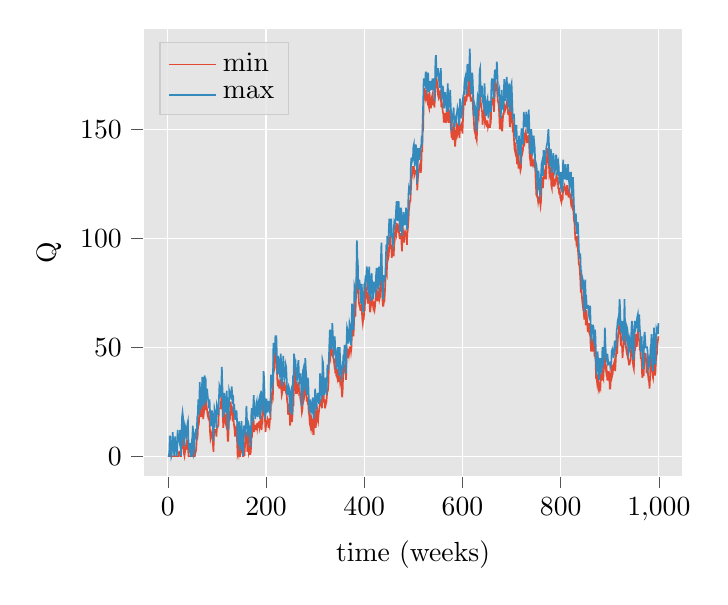
\begin{tikzpicture}

\definecolor{color0}{rgb}{0.886274509803922,0.290196078431373,0.2}
\definecolor{color1}{rgb}{0.203921568627451,0.541176470588235,0.741176470588235}

\begin{axis}[
axis background/.style={fill=white!89.8039215686275!black},
axis line style={white},
legend cell align={left},
legend style={fill opacity=0.8, draw opacity=1, text opacity=1, at={(0.03,0.97)}, anchor=north west, draw=white!80!black, fill=white!89.8039215686275!black},
tick align=outside,
tick pos=left,
x grid style={white},
xlabel={time (weeks)},
xmajorgrids,
xmin=-49.95, xmax=1048.95,
xtick style={color=white!33.3333333333333!black},
y grid style={white},
ylabel={Q},
ymajorgrids,
ymin=-9.35, ymax=196.35,
ytick style={color=white!33.3333333333333!black}
]
\addplot [semithick, color0]
table {%
0 0
1 0
2 0
3 0
4 0
5 1
6 0
7 0
8 0
9 0
10 0
11 0
12 0
13 0
14 0
15 0
16 0
17 0
18 0
19 0
20 0
21 0
22 0
23 2
24 2
25 1
26 0
27 0
28 7
29 6
30 15
31 15
32 8
33 1
34 0
35 2
36 3
37 5
38 6
39 7
40 3
41 6
42 0
43 0
44 0
45 0
46 0
47 0
48 0
49 0
50 0
51 7
52 0
53 0
54 0
55 0
56 2
57 2
58 4
59 8
60 8
61 10
62 18
63 14
64 18
65 24
66 19
67 21
68 18
69 20
70 26
71 27
72 17
73 19
74 21
75 27
76 25
77 28
78 21
79 23
80 21
81 19
82 18
83 19
84 18
85 16
86 11
87 8
88 9
89 10
90 11
91 10
92 5
93 2
94 10
95 12
96 12
97 12
98 11
99 9
100 13
101 13
102 14
103 14
104 22
105 22
106 22
107 22
108 22
109 29
110 31
111 24
112 18
113 13
114 16
115 19
116 18
117 16
118 15
119 19
120 20
121 13
122 7
123 7
124 13
125 20
126 20
127 19
128 25
129 22
130 22
131 20
132 16
133 23
134 16
135 14
136 12
137 9
138 12
139 13
140 11
141 7
142 1
143 2
144 1
145 6
146 0
147 0
148 2
149 4
150 8
151 5
152 2
153 0
154 0
155 2
156 0
157 4
158 11
159 9
160 11
161 8
162 2
163 11
164 9
165 2
166 3
167 1
168 1
169 2
170 7
171 12
172 11
173 14
174 17
175 16
176 11
177 14
178 14
179 14
180 12
181 15
182 13
183 15
184 15
185 13
186 16
187 13
188 14
189 18
190 18
191 12
192 18
193 17
194 22
195 27
196 26
197 22
198 16
199 11
200 14
201 16
202 16
203 17
204 16
205 13
206 15
207 14
208 17
209 17
210 25
211 27
212 26
213 29
214 28
215 40
216 39
217 40
218 45
219 49
220 43
221 45
222 40
223 35
224 32
225 34
226 33
227 31
228 34
229 35
230 35
231 31
232 28
233 29
234 31
235 34
236 30
237 32
238 33
239 31
240 30
241 31
242 29
243 25
244 24
245 19
246 22
247 24
248 19
249 14
250 17
251 20
252 16
253 16
254 19
255 25
256 23
257 40
258 42
259 38
260 32
261 29
262 29
263 32
264 31
265 30
266 34
267 31
268 31
269 29
270 26
271 25
272 23
273 20
274 21
275 27
276 30
277 26
278 27
279 32
280 33
281 30
282 30
283 25
284 27
285 24
286 24
287 20
288 19
289 15
290 14
291 13
292 18
293 17
294 14
295 15
296 10
297 10
298 18
299 18
300 19
301 13
302 15
303 20
304 21
305 17
306 16
307 19
308 21
309 23
310 26
311 23
312 25
313 24
314 22
315 32
316 33
317 31
318 25
319 25
320 22
321 26
322 24
323 25
324 28
325 30
326 30
327 33
328 42
329 46
330 46
331 45
332 51
333 46
334 49
335 49
336 46
337 45
338 44
339 42
340 43
341 38
342 40
343 37
344 37
345 36
346 40
347 36
348 34
349 37
350 38
351 34
352 35
353 34
354 30
355 27
356 30
357 37
358 40
359 41
360 39
361 39
362 38
363 35
364 46
365 47
366 48
367 45
368 49
369 47
370 49
371 50
372 50
373 48
374 50
375 58
376 56
377 57
378 55
379 60
380 66
381 67
382 64
383 72
384 77
385 87
386 81
387 82
388 74
389 71
390 69
391 69
392 67
393 67
394 69
395 67
396 63
397 61
398 63
399 63
400 67
401 67
402 74
403 80
404 74
405 75
406 75
407 70
408 73
409 72
410 75
411 69
412 66
413 68
414 71
415 72
416 69
417 71
418 69
419 71
420 68
421 67
422 69
423 72
424 77
425 74
426 76
427 71
428 74
429 74
430 75
431 72
432 73
433 79
434 85
435 86
436 77
437 72
438 69
439 69
440 71
441 71
442 75
443 80
444 85
445 85
446 84
447 94
448 96
449 91
450 92
451 99
452 100
453 101
454 95
455 97
456 91
457 93
458 94
459 92
460 92
461 97
462 99
463 104
464 103
465 102
466 107
467 104
468 105
469 104
470 105
471 102
472 100
473 100
474 102
475 102
476 97
477 94
478 106
479 103
480 100
481 98
482 102
483 103
484 102
485 102
486 100
487 97
488 106
489 105
490 108
491 113
492 115
493 117
494 117
495 122
496 127
497 128
498 133
499 130
500 130
501 133
502 129
503 130
504 131
505 131
506 131
507 128
508 122
509 127
510 129
511 131
512 132
513 133
514 134
515 130
516 132
517 140
518 140
519 149
520 150
521 163
522 166
523 169
524 165
525 164
526 166
527 168
528 165
529 163
530 164
531 161
532 160
533 167
534 162
535 160
536 160
537 164
538 165
539 166
540 161
541 163
542 162
543 160
544 165
545 170
546 174
547 171
548 172
549 170
550 166
551 165
552 167
553 166
554 165
555 164
556 168
557 160
558 162
559 160
560 158
561 157
562 153
563 157
564 157
565 155
566 153
567 156
568 155
569 157
570 159
571 155
572 153
573 158
574 157
575 156
576 152
577 149
578 146
579 151
580 145
581 147
582 153
583 151
584 145
585 142
586 145
587 146
588 153
589 152
590 148
591 149
592 151
593 149
594 146
595 152
596 152
597 151
598 152
599 151
600 148
601 154
602 159
603 163
604 165
605 161
606 164
607 163
608 163
609 165
610 168
611 167
612 165
613 172
614 174
615 175
616 165
617 163
618 163
619 163
620 164
621 162
622 157
623 155
624 150
625 149
626 150
627 146
628 146
629 145
630 150
631 155
632 157
633 156
634 161
635 165
636 168
637 160
638 162
639 159
640 158
641 152
642 157
643 158
644 154
645 159
646 153
647 154
648 153
649 153
650 151
651 154
652 151
653 152
654 152
655 151
656 151
657 156
658 155
659 165
660 161
661 163
662 163
663 164
664 158
665 162
666 167
667 170
668 171
669 169
670 169
671 166
672 163
673 162
674 161
675 156
676 150
677 153
678 152
679 156
680 156
681 149
682 154
683 157
684 157
685 161
686 160
687 159
688 160
689 161
690 162
691 160
692 160
693 157
694 157
695 159
696 153
697 151
698 161
699 164
700 159
701 155
702 151
703 152
704 149
705 145
706 141
707 140
708 144
709 140
710 140
711 134
712 137
713 138
714 132
715 135
716 134
717 133
718 131
719 132
720 138
721 140
722 139
723 140
724 144
725 146
726 142
727 148
728 148
729 149
730 146
731 144
732 144
733 145
734 147
735 147
736 142
737 137
738 136
739 133
740 138
741 137
742 133
743 136
744 134
745 135
746 134
747 135
748 133
749 127
750 122
751 123
752 119
753 119
754 117
755 119
756 116
757 118
758 117
759 115
760 117
761 124
762 128
763 126
764 123
765 128
766 130
767 127
768 131
769 132
770 127
771 132
772 136
773 141
774 141
775 138
776 134
777 129
778 130
779 131
780 129
781 124
782 123
783 130
784 131
785 127
786 124
787 124
788 127
789 127
790 126
791 128
792 129
793 126
794 128
795 123
796 123
797 120
798 123
799 119
800 118
801 120
802 117
803 118
804 118
805 124
806 122
807 123
808 124
809 123
810 122
811 120
812 120
813 124
814 124
815 122
816 119
817 119
818 121
819 120
820 118
821 120
822 116
823 117
824 115
825 116
826 112
827 108
828 108
829 103
830 99
831 101
832 98
833 99
834 101
835 95
836 92
837 88
838 88
839 85
840 81
841 75
842 78
843 74
844 71
845 69
846 70
847 66
848 63
849 63
850 69
851 60
852 67
853 65
854 62
855 57
856 59
857 58
858 61
859 59
860 57
861 51
862 48
863 51
864 52
865 48
866 50
867 52
868 50
869 46
870 46
871 44
872 36
873 36
874 34
875 36
876 35
877 31
878 32
879 31
880 33
881 32
882 38
883 35
884 35
885 38
886 37
887 36
888 41
889 43
890 47
891 42
892 40
893 42
894 38
895 35
896 35
897 35
898 39
899 37
900 31
901 31
902 35
903 40
904 42
905 37
906 38
907 41
908 42
909 43
910 41
911 39
912 43
913 48
914 52
915 47
916 52
917 56
918 57
919 60
920 60
921 58
922 53
923 54
924 51
925 50
926 45
927 49
928 50
929 55
930 60
931 51
932 53
933 50
934 48
935 47
936 48
937 45
938 44
939 42
940 42
941 43
942 44
943 47
944 52
945 50
946 49
947 43
948 41
949 40
950 46
951 52
952 51
953 56
954 53
955 50
956 54
957 58
958 54
959 54
960 53
961 49
962 49
963 45
964 45
965 43
966 36
967 38
968 37
969 37
970 43
971 47
972 47
973 47
974 44
975 38
976 40
977 41
978 37
979 35
980 34
981 31
982 36
983 47
984 45
985 44
986 40
987 37
988 36
989 43
990 47
991 43
992 37
993 39
994 44
995 46
996 47
997 51
998 53
999 55
};
\addlegendentry{min}
\addplot [semithick, color1]
table {%
0 0
1 0
2 0
3 2
4 9
5 9
6 3
7 0
8 1
9 4
10 11
11 6
12 4
13 0
14 5
15 9
16 5
17 3
18 0
19 2
20 12
21 9
22 8
23 7
24 6
25 12
26 7
27 0
28 11
29 18
30 20
31 18
32 8
33 5
34 5
35 14
36 13
37 12
38 10
39 12
40 15
41 16
42 7
43 4
44 3
45 6
46 4
47 0
48 0
49 7
50 9
51 14
52 4
53 1
54 2
55 10
56 11
57 10
58 9
59 12
60 18
61 19
62 26
63 19
64 22
65 34
66 28
67 29
68 23
69 24
70 36
71 36
72 25
73 24
74 25
75 37
76 34
77 36
78 26
79 27
80 31
81 28
82 26
83 24
84 22
85 26
86 20
87 16
88 14
89 14
90 21
91 19
92 13
93 7
94 14
95 22
96 21
97 20
98 16
99 13
100 23
101 22
102 22
103 19
104 26
105 32
106 31
107 30
108 27
109 33
110 41
111 33
112 26
113 18
114 20
115 29
116 27
117 24
118 20
119 23
120 30
121 22
122 15
123 12
124 17
125 30
126 29
127 27
128 30
129 26
130 32
131 29
132 24
133 28
134 20
135 24
136 21
137 17
138 17
139 17
140 21
141 16
142 9
143 7
144 5
145 16
146 9
147 3
148 3
149 13
150 16
151 11
152 5
153 0
154 6
155 14
156 10
157 11
158 14
159 15
160 23
161 18
162 9
163 14
164 15
165 14
166 13
167 8
168 4
169 8
170 19
171 22
172 18
173 17
174 23
175 28
176 21
177 21
178 17
179 20
180 24
181 25
182 20
183 18
184 21
185 25
186 26
187 20
188 17
189 24
190 30
191 22
192 25
193 20
194 28
195 39
196 36
197 29
198 19
199 17
200 26
201 26
202 23
203 20
204 22
205 25
206 25
207 21
208 20
209 23
210 37
211 37
212 33
213 32
214 34
215 52
216 49
217 47
218 48
219 55
220 55
221 55
222 47
223 38
224 38
225 46
226 43
227 38
228 37
229 41
230 47
231 41
232 35
233 32
234 37
235 46
236 40
237 39
238 36
239 37
240 42
241 41
242 36
243 28
244 30
245 31
246 32
247 31
248 22
249 20
250 29
251 30
252 23
253 19
254 25
255 37
256 33
257 47
258 45
259 44
260 44
261 39
262 36
263 35
264 37
265 42
266 44
267 38
268 34
269 35
270 38
271 35
272 30
273 23
274 27
275 39
276 40
277 33
278 30
279 38
280 45
281 40
282 37
283 28
284 33
285 36
286 34
287 27
288 22
289 21
290 26
291 23
292 25
293 20
294 20
295 27
296 20
297 17
298 21
299 24
300 31
301 23
302 22
303 23
304 27
305 29
306 26
307 26
308 24
309 29
310 38
311 33
312 32
313 27
314 28
315 44
316 43
317 38
318 28
319 31
320 34
321 36
322 31
323 28
324 34
325 42
326 40
327 40
328 45
329 52
330 58
331 55
332 58
333 49
334 55
335 61
336 56
337 52
338 47
339 48
340 55
341 48
342 47
343 40
344 43
345 48
346 50
347 43
348 37
349 43
350 50
351 44
352 42
353 37
354 36
355 39
356 40
357 44
358 43
359 47
360 51
361 49
362 45
363 38
364 52
365 59
366 58
367 52
368 52
369 53
370 61
371 60
372 57
373 51
374 56
375 70
376 66
377 64
378 58
379 66
380 78
381 77
382 71
383 75
384 83
385 99
386 91
387 89
388 77
389 77
390 81
391 79
392 74
393 70
394 75
395 79
396 73
397 68
398 66
399 69
400 79
401 77
402 81
403 83
404 80
405 87
406 85
407 77
408 76
409 78
410 87
411 79
412 73
413 71
414 77
415 84
416 79
417 78
418 72
419 77
420 80
421 77
422 76
423 75
424 83
425 86
426 86
427 78
428 77
429 80
430 87
431 82
432 80
433 82
434 91
435 98
436 87
437 79
438 72
439 75
440 83
441 81
442 82
443 83
444 91
445 97
446 94
447 101
448 99
449 97
450 104
451 109
452 107
453 104
454 101
455 109
456 101
457 100
458 97
459 98
460 104
461 107
462 106
463 107
464 109
465 114
466 117
467 111
468 108
469 110
470 117
471 112
472 107
473 103
474 108
475 114
476 107
477 101
478 109
479 109
480 112
481 108
482 109
483 106
484 108
485 114
486 110
487 104
488 109
489 111
490 120
491 123
492 122
493 120
494 123
495 134
496 137
497 135
498 136
499 136
500 142
501 143
502 136
503 133
504 137
505 143
506 141
507 135
508 125
509 133
510 141
511 141
512 139
513 136
514 140
515 142
516 142
517 147
518 143
519 155
520 162
521 173
522 173
523 172
524 171
525 176
526 176
527 175
528 168
529 169
530 176
531 171
532 167
533 170
534 168
535 172
536 170
537 171
538 168
539 172
540 173
541 173
542 169
543 163
544 171
545 182
546 184
547 178
548 175
549 176
550 178
551 175
552 174
553 169
554 171
555 176
556 178
557 167
558 165
559 166
560 170
561 167
562 160
563 160
564 163
565 167
566 163
567 163
568 158
569 163
570 171
571 165
572 160
573 161
574 163
575 168
576 162
577 156
578 149
579 157
580 157
581 157
582 160
583 154
584 151
585 154
586 155
587 153
588 156
589 158
590 160
591 159
592 158
593 152
594 152
595 164
596 162
597 158
598 155
599 157
600 160
601 164
602 166
603 166
604 171
605 173
606 174
607 170
608 166
609 171
610 180
611 177
612 172
613 175
614 180
615 187
616 175
617 170
618 166
619 169
620 176
621 172
622 164
623 158
624 156
625 161
626 160
627 153
628 149
629 151
630 162
631 165
632 164
633 159
634 167
635 177
636 178
637 167
638 165
639 165
640 170
641 162
642 164
643 161
644 160
645 171
646 163
647 161
648 156
649 159
650 163
651 164
652 158
653 155
654 158
655 163
656 161
657 163
658 158
659 171
660 173
661 173
662 170
663 167
664 164
665 174
666 177
667 177
668 174
669 175
670 181
671 176
672 170
673 165
674 167
675 168
676 160
677 160
678 155
679 162
680 168
681 159
682 161
683 160
684 163
685 173
686 170
687 166
688 163
689 167
690 174
691 170
692 167
693 160
694 163
695 171
696 163
697 158
698 164
699 170
700 171
701 165
702 158
703 155
704 155
705 157
706 151
707 147
708 147
709 146
710 152
711 144
712 144
713 141
714 138
715 147
716 144
717 140
718 134
719 138
720 150
721 150
722 146
723 143
724 150
725 158
726 152
727 155
728 151
729 155
730 158
731 154
732 151
733 148
734 153
735 159
736 152
737 144
738 139
739 139
740 150
741 147
742 140
743 139
744 140
745 147
746 144
747 142
748 136
749 133
750 134
751 133
752 126
753 122
754 123
755 131
756 126
757 125
758 120
759 121
760 129
761 134
762 135
763 129
764 129
765 140
766 140
767 134
768 134
769 138
770 139
771 142
772 143
773 144
774 147
775 150
776 144
777 136
778 133
779 137
780 141
781 134
782 130
783 133
784 137
785 139
786 134
787 131
788 130
789 133
790 138
791 138
792 136
793 129
794 134
795 135
796 133
797 127
798 126
799 125
800 130
801 130
802 124
803 121
804 124
805 136
806 132
807 130
808 127
809 129
810 134
811 130
812 127
813 127
814 130
815 134
816 129
817 126
818 124
819 126
820 130
821 130
822 123
823 120
824 121
825 128
826 122
827 115
828 111
829 109
830 111
831 111
832 105
833 102
834 107
835 107
836 102
837 95
838 91
839 91
840 93
841 85
842 85
843 77
844 77
845 81
846 80
847 73
848 66
849 69
850 81
851 70
852 74
853 68
854 68
855 69
856 69
857 65
858 64
859 65
860 69
861 61
862 55
863 54
864 58
865 60
866 60
867 59
868 53
869 52
870 58
871 54
872 43
873 39
874 40
875 48
876 45
877 38
878 35
879 37
880 45
881 42
882 45
883 38
884 41
885 50
886 47
887 43
888 44
889 49
890 59
891 52
892 47
893 45
894 44
895 47
896 45
897 42
898 42
899 43
900 43
901 41
902 42
903 43
904 48
905 49
906 48
907 48
908 45
909 49
910 53
911 49
912 50
913 51
914 58
915 59
916 62
917 63
918 60
919 66
920 72
921 68
922 60
923 57
924 57
925 62
926 55
927 56
928 53
929 61
930 72
931 61
932 60
933 53
934 54
935 59
936 58
937 52
938 47
939 48
940 54
941 53
942 51
943 50
944 58
945 62
946 59
947 50
948 44
949 46
950 58
951 62
952 58
953 59
954 59
955 62
956 64
957 65
958 57
959 60
960 65
961 59
962 56
963 48
964 51
965 55
966 46
967 45
968 40
969 43
970 55
971 57
972 54
973 50
974 50
975 50
976 50
977 48
978 40
979 41
980 46
981 41
982 43
983 50
984 51
985 56
986 50
987 44
988 39
989 49
990 59
991 53
992 44
993 42
994 50
995 58
996 57
997 58
998 56
999 61
};
\addlegendentry{max}
\end{axis}

\end{tikzpicture}
 
\caption{Effect of capacity and holiday plans. We plot for each time point
  the maximum and the minimum queue length for each of the
  policies. Apparently, the effect of each of these policies is, for
  all practical purposes, negligible.  }
\label{fig:balanced}
\end{figure}


Now we consider Suggestion 3, which comes down to doing more intakes when it is busy, and fewer when it is quiet.
A simple rule would be to use week's queue $L_{n-1}$: if $L_{n-1}<12$, serve $e$ intakes less (in other, when the service capacity of week~$k$ is larger than the queue length serve $e$ less), when $L_{n-1}>24$, serve~$e$ more.
Here, $e=1$ or $2$, or perhaps a larger number.
The larger $e$, the larger the control we exercise.

Let's consider three different control levels, $e=1$, $e=2$, and $e=5$; thus in the last case all psychiatrists do five extra intakes.
The previous simulation shows that it is safe to disregard the holiday plans, so just assume a flat service capacity of 12 intakes a week.
The results, see~\cref{fig:intakes}, show a striking difference indeed.
The queue does not explode anymore, and already taking $e=1$ has a large influence.


\begin{figure}[ht]
  \centering
% progs/intake_control.py
% This file was created by tikzplotlib v0.9.1.
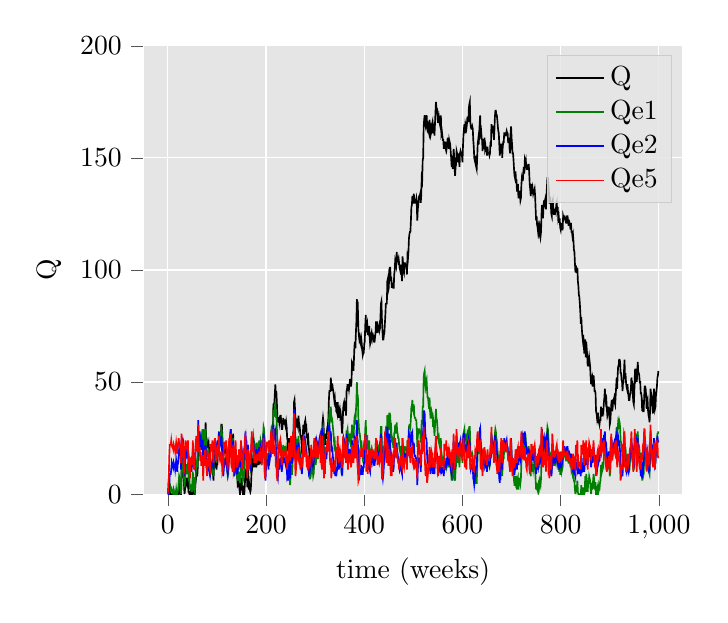
\begin{tikzpicture}

\begin{axis}[
axis background/.style={fill=white!89.8039215686275!black},
axis line style={white},
legend cell align={left},
legend style={fill opacity=0.8, draw opacity=1, text opacity=1, draw=white!80!black, fill=white!89.8039215686275!black},
tick align=outside,
tick pos=left,
x grid style={white},
xlabel={time (weeks)},
xmajorgrids,
xmin=-49.95, xmax=1048.95,
xtick style={color=white!33.3333333333333!black},
y grid style={white},
ylabel={Q},
ymajorgrids,
ymin=0, ymax=200,
ytick style={color=white!33.3333333333333!black}
]
\addplot [semithick, black]
table {%
0 0
1 0
2 0
3 1
4 3
5 0
6 0
7 0
8 0
9 0
10 0
11 0
12 1
13 0
14 0
15 0
16 0
17 1
18 0
19 0
20 0
21 0
22 2
23 4
24 2
25 0
26 0
27 0
28 10
29 12
30 14
31 15
32 8
33 4
34 0
35 2
36 4
37 6
38 7
39 7
40 3
41 7
42 1
43 1
44 0
45 0
46 1
47 0
48 0
49 1
50 0
51 8
52 1
53 1
54 0
55 0
56 4
57 6
58 8
59 10
60 8
61 12
62 22
63 18
64 20
65 24
66 21
67 25
68 22
69 22
70 26
71 29
72 21
73 23
74 23
75 27
76 27
77 32
78 25
79 25
80 21
81 21
82 22
83 23
84 20
85 16
86 13
87 12
88 13
89 12
90 11
91 12
92 9
93 6
94 12
95 12
96 14
97 16
98 15
99 11
100 13
101 15
102 18
103 18
104 24
105 22
106 24
107 26
108 26
109 31
110 31
111 26
112 22
113 17
114 18
115 19
116 20
117 20
118 19
119 21
120 20
121 15
122 11
123 11
124 15
125 20
126 22
127 23
128 29
129 24
130 22
131 22
132 20
133 27
134 18
135 14
136 14
137 13
138 16
139 15
140 11
141 9
142 5
143 6
144 3
145 6
146 2
147 0
148 2
149 7
150 7
151 5
152 2
153 0
154 0
155 2
156 1
157 5
158 11
159 9
160 11
161 9
162 3
163 11
164 9
165 2
166 4
167 2
168 1
169 2
170 7
171 13
172 12
173 14
174 17
175 16
176 12
177 15
178 14
179 14
180 12
181 16
182 14
183 15
184 15
185 13
186 17
187 14
188 14
189 18
190 18
191 13
192 19
193 17
194 22
195 27
196 27
197 23
198 16
199 11
200 14
201 17
202 17
203 17
204 16
205 13
206 16
207 15
208 17
209 17
210 25
211 28
212 27
213 29
214 28
215 40
216 40
217 41
218 45
219 49
220 43
221 46
222 41
223 35
224 32
225 34
226 34
227 32
228 34
229 35
230 35
231 32
232 29
233 29
234 31
235 34
236 31
237 33
238 33
239 31
240 30
241 32
242 30
243 25
244 24
245 19
246 23
247 25
248 19
249 14
250 17
251 21
252 17
253 16
254 19
255 25
256 24
257 41
258 42
259 38
260 32
261 30
262 30
263 32
264 31
265 30
266 35
267 32
268 31
269 29
270 26
271 26
272 24
273 20
274 21
275 27
276 31
277 27
278 27
279 32
280 33
281 31
282 31
283 25
284 27
285 24
286 25
287 21
288 19
289 15
290 14
291 14
292 19
293 17
294 14
295 15
296 11
297 11
298 18
299 18
300 19
301 14
302 16
303 20
304 21
305 17
306 17
307 20
308 21
309 23
310 26
311 24
312 26
313 24
314 22
315 32
316 34
317 32
318 25
319 25
320 22
321 27
322 25
323 25
324 28
325 30
326 31
327 34
328 42
329 46
330 46
331 46
332 52
333 46
334 49
335 49
336 47
337 46
338 44
339 42
340 43
341 39
342 41
343 37
344 37
345 36
346 41
347 37
348 34
349 37
350 38
351 35
352 36
353 34
354 30
355 27
356 31
357 38
358 40
359 41
360 39
361 40
362 39
363 35
364 46
365 47
366 49
367 46
368 49
369 47
370 49
371 51
372 51
373 48
374 50
375 58
376 57
377 58
378 55
379 60
380 66
381 68
382 65
383 72
384 77
385 87
386 82
387 83
388 74
389 71
390 69
391 70
392 68
393 67
394 69
395 67
396 64
397 62
398 63
399 63
400 67
401 68
402 75
403 80
404 74
405 75
406 76
407 71
408 73
409 72
410 75
411 70
412 67
413 68
414 71
415 72
416 70
417 72
418 69
419 71
420 68
421 68
422 70
423 72
424 77
425 74
426 77
427 72
428 74
429 74
430 75
431 73
432 74
433 79
434 85
435 86
436 78
437 73
438 69
439 69
440 71
441 72
442 76
443 80
444 85
445 85
446 85
447 95
448 96
449 91
450 92
451 100
452 101
453 101
454 95
455 97
456 92
457 94
458 94
459 92
460 92
461 98
462 100
463 104
464 103
465 102
466 108
467 105
468 105
469 104
470 105
471 103
472 101
473 100
474 102
475 102
476 98
477 95
478 106
479 103
480 100
481 99
482 103
483 103
484 102
485 102
486 101
487 98
488 106
489 105
490 108
491 114
492 116
493 117
494 117
495 122
496 128
497 129
498 133
499 130
500 130
501 134
502 130
503 130
504 131
505 131
506 132
507 129
508 122
509 127
510 129
511 132
512 133
513 133
514 134
515 130
516 133
517 141
518 140
519 149
520 150
521 164
522 167
523 169
524 165
525 164
526 167
527 169
528 165
529 163
530 164
531 162
532 161
533 167
534 162
535 160
536 161
537 165
538 165
539 166
540 161
541 164
542 163
543 160
544 165
545 170
546 175
547 172
548 172
549 170
550 166
551 166
552 168
553 166
554 165
555 164
556 169
557 161
558 162
559 160
560 158
561 158
562 154
563 157
564 157
565 155
566 154
567 157
568 155
569 157
570 159
571 156
572 154
573 158
574 157
575 156
576 153
577 150
578 146
579 151
580 145
581 148
582 154
583 151
584 145
585 142
586 146
587 147
588 153
589 152
590 148
591 150
592 152
593 149
594 146
595 152
596 153
597 152
598 152
599 151
600 148
601 155
602 160
603 163
604 165
605 161
606 165
607 164
608 163
609 165
610 168
611 168
612 166
613 172
614 174
615 175
616 166
617 164
618 163
619 163
620 164
621 163
622 158
623 155
624 150
625 149
626 151
627 147
628 146
629 145
630 150
631 156
632 158
633 156
634 161
635 165
636 169
637 161
638 162
639 159
640 158
641 153
642 158
643 158
644 154
645 159
646 154
647 155
648 153
649 153
650 151
651 155
652 152
653 152
654 152
655 151
656 152
657 157
658 155
659 165
660 161
661 164
662 164
663 164
664 158
665 162
666 168
667 171
668 171
669 169
670 169
671 167
672 164
673 162
674 161
675 156
676 151
677 154
678 152
679 156
680 156
681 150
682 155
683 157
684 157
685 161
686 161
687 160
688 160
689 161
690 162
691 161
692 161
693 157
694 157
695 159
696 154
697 152
698 161
699 164
700 159
701 156
702 152
703 152
704 149
705 145
706 142
707 141
708 144
709 140
710 140
711 135
712 138
713 138
714 132
715 135
716 135
717 134
718 131
719 132
720 138
721 141
722 140
723 140
724 144
725 146
726 143
727 149
728 148
729 149
730 146
731 145
732 145
733 145
734 147
735 147
736 143
737 138
738 136
739 133
740 138
741 138
742 134
743 136
744 134
745 135
746 135
747 136
748 133
749 127
750 122
751 124
752 120
753 119
754 117
755 119
756 117
757 119
758 117
759 115
760 117
761 125
762 129
763 126
764 123
765 128
766 131
767 128
768 131
769 132
770 127
771 133
772 137
773 141
774 141
775 138
776 135
777 130
778 130
779 131
780 129
781 125
782 124
783 130
784 131
785 127
786 125
787 125
788 127
789 127
790 126
791 129
792 130
793 126
794 128
795 123
796 124
797 121
798 123
799 119
800 118
801 121
802 118
803 118
804 118
805 124
806 123
807 124
808 124
809 123
810 122
811 121
812 121
813 124
814 124
815 122
816 120
817 120
818 121
819 120
820 118
821 121
822 117
823 117
824 115
825 116
826 113
827 109
828 108
829 103
830 99
831 102
832 99
833 99
834 101
835 95
836 93
837 89
838 88
839 85
840 81
841 76
842 79
843 74
844 71
845 69
846 71
847 67
848 63
849 63
850 69
851 61
852 68
853 65
854 62
855 57
856 60
857 59
858 61
859 59
860 57
861 52
862 49
863 51
864 52
865 48
866 51
867 53
868 50
869 46
870 46
871 45
872 37
873 36
874 34
875 36
876 36
877 32
878 32
879 31
880 33
881 33
882 39
883 35
884 35
885 38
886 38
887 37
888 41
889 43
890 47
891 43
892 41
893 42
894 38
895 35
896 36
897 36
898 39
899 37
900 31
901 32
902 36
903 40
904 42
905 37
906 39
907 42
908 42
909 43
910 41
911 40
912 44
913 48
914 52
915 47
916 53
917 57
918 57
919 60
920 60
921 59
922 54
923 54
924 51
925 50
926 46
927 50
928 50
929 55
930 60
931 52
932 54
933 50
934 48
935 47
936 49
937 46
938 44
939 42
940 42
941 44
942 45
943 47
944 52
945 50
946 50
947 44
948 41
949 40
950 46
951 53
952 52
953 56
954 53
955 50
956 55
957 59
958 54
959 54
960 53
961 50
962 50
963 45
964 45
965 43
966 37
967 39
968 37
969 37
970 43
971 48
972 48
973 47
974 44
975 38
976 41
977 42
978 37
979 35
980 34
981 32
982 37
983 47
984 45
985 44
986 41
987 38
988 36
989 43
990 47
991 44
992 38
993 39
994 44
995 46
996 48
997 52
998 53
999 55
};
\addlegendentry{Q}
\addplot [semithick, green!50.1960784313725!black]
table {%
0 0
1 0
2 0
3 2
4 5
5 3
6 1
7 1
8 2
9 1
10 1
11 0
12 2
13 1
14 1
15 0
16 0
17 2
18 0
19 0
20 1
21 2
22 5
23 8
24 7
25 6
26 5
27 0
28 11
29 14
30 16
31 17
32 10
33 7
34 3
35 6
36 9
37 12
38 13
39 13
40 9
41 14
42 8
43 9
44 7
45 2
46 4
47 4
48 1
49 3
50 1
51 10
52 4
53 5
54 2
55 1
56 6
57 9
58 12
59 14
60 12
61 16
62 26
63 21
64 23
65 27
66 23
67 27
68 23
69 23
70 27
71 29
72 20
73 22
74 22
75 26
76 25
77 29
78 21
79 21
80 17
81 17
82 18
83 19
84 16
85 12
86 9
87 9
88 11
89 11
90 11
91 13
92 10
93 8
94 15
95 15
96 17
97 19
98 18
99 14
100 16
101 18
102 21
103 21
104 27
105 24
106 25
107 26
108 25
109 29
110 28
111 22
112 18
113 13
114 14
115 15
116 16
117 16
118 15
119 17
120 16
121 11
122 8
123 9
124 14
125 19
126 21
127 22
128 28
129 22
130 20
131 20
132 18
133 25
134 15
135 11
136 12
137 11
138 15
139 14
140 10
141 9
142 6
143 8
144 6
145 10
146 7
147 5
148 8
149 14
150 14
151 12
152 9
153 6
154 7
155 10
156 10
157 15
158 21
159 19
160 21
161 19
162 13
163 21
164 19
165 12
166 14
167 12
168 11
169 13
170 18
171 24
172 22
173 24
174 26
175 24
176 19
177 22
178 21
179 21
180 19
181 23
182 21
183 22
184 22
185 20
186 24
187 20
188 20
189 24
190 23
191 18
192 24
193 21
194 26
195 30
196 29
197 24
198 16
199 11
200 15
201 18
202 18
203 18
204 17
205 14
206 17
207 16
208 18
209 18
210 26
211 28
212 26
213 27
214 25
215 36
216 35
217 35
218 38
219 41
220 34
221 36
222 30
223 23
224 20
225 22
226 22
227 20
228 22
229 23
230 23
231 20
232 17
233 17
234 19
235 22
236 19
237 21
238 21
239 19
240 18
241 20
242 18
243 13
244 12
245 7
246 12
247 14
248 8
249 4
250 8
251 13
252 9
253 9
254 13
255 19
256 18
257 35
258 35
259 30
260 23
261 21
262 21
263 23
264 22
265 21
266 26
267 22
268 21
269 19
270 16
271 16
272 14
273 10
274 12
275 18
276 22
277 18
278 18
279 23
280 24
281 21
282 21
283 15
284 17
285 14
286 15
287 11
288 10
289 7
290 7
291 8
292 14
293 12
294 9
295 11
296 8
297 9
298 17
299 17
300 18
301 13
302 15
303 19
304 20
305 16
306 16
307 19
308 20
309 22
310 25
311 22
312 24
313 21
314 19
315 29
316 30
317 27
318 19
319 19
320 16
321 21
322 19
323 19
324 22
325 24
326 24
327 26
328 33
329 36
330 35
331 34
332 39
333 32
334 34
335 33
336 30
337 28
338 25
339 22
340 23
341 19
342 21
343 17
344 17
345 16
346 21
347 17
348 14
349 17
350 18
351 15
352 16
353 14
354 10
355 8
356 13
357 20
358 22
359 23
360 21
361 22
362 21
363 17
364 28
365 28
366 29
367 25
368 27
369 24
370 25
371 26
372 25
373 21
374 23
375 31
376 29
377 29
378 25
379 29
380 34
381 35
382 31
383 37
384 41
385 50
386 44
387 44
388 34
389 30
390 27
391 27
392 24
393 22
394 24
395 21
396 18
397 16
398 17
399 17
400 21
401 22
402 29
403 33
404 26
405 26
406 26
407 20
408 22
409 21
410 24
411 18
412 15
413 16
414 19
415 20
416 18
417 20
418 17
419 19
420 16
421 16
422 18
423 20
424 25
425 21
426 24
427 18
428 20
429 20
430 21
431 19
432 20
433 25
434 30
435 30
436 21
437 16
438 12
439 12
440 14
441 15
442 19
443 23
444 28
445 27
446 26
447 35
448 35
449 29
450 29
451 36
452 36
453 35
454 28
455 29
456 23
457 25
458 24
459 21
460 21
461 27
462 28
463 31
464 29
465 27
466 32
467 28
468 27
469 25
470 25
471 22
472 20
473 19
474 21
475 21
476 17
477 14
478 25
479 21
480 18
481 17
482 21
483 21
484 20
485 20
486 19
487 16
488 24
489 22
490 25
491 30
492 31
493 31
494 30
495 34
496 39
497 39
498 42
499 38
500 37
501 40
502 35
503 34
504 34
505 33
506 33
507 29
508 21
509 26
510 27
511 29
512 29
513 28
514 28
515 23
516 26
517 33
518 31
519 39
520 39
521 52
522 54
523 55
524 50
525 48
526 50
527 51
528 46
529 43
530 43
531 40
532 38
533 43
534 37
535 34
536 34
537 37
538 36
539 36
540 30
541 32
542 30
543 26
544 30
545 34
546 38
547 34
548 33
549 30
550 25
551 24
552 25
553 22
554 21
555 20
556 25
557 16
558 17
559 15
560 13
561 13
562 9
563 13
564 13
565 11
566 11
567 15
568 13
569 15
570 17
571 14
572 12
573 16
574 15
575 14
576 11
577 9
578 6
579 12
580 6
581 10
582 17
583 14
584 8
585 6
586 11
587 13
588 19
589 18
590 14
591 16
592 18
593 15
594 12
595 18
596 19
597 18
598 18
599 17
600 14
601 21
602 26
603 28
604 29
605 24
606 27
607 25
608 23
609 25
610 27
611 26
612 23
613 29
614 30
615 30
616 20
617 18
618 17
619 17
620 18
621 17
622 12
623 9
624 5
625 5
626 8
627 5
628 5
629 5
630 11
631 18
632 20
633 18
634 23
635 27
636 30
637 21
638 22
639 19
640 18
641 13
642 18
643 18
644 14
645 19
646 14
647 15
648 13
649 13
650 11
651 16
652 13
653 13
654 13
655 12
656 13
657 18
658 16
659 26
660 21
661 24
662 23
663 23
664 17
665 21
666 27
667 29
668 28
669 25
670 24
671 21
672 18
673 16
674 15
675 10
676 6
677 10
678 9
679 14
680 14
681 8
682 14
683 16
684 16
685 20
686 20
687 19
688 19
689 20
690 21
691 20
692 20
693 16
694 16
695 18
696 13
697 11
698 21
699 24
700 18
701 15
702 11
703 12
704 9
705 6
706 4
707 4
708 8
709 5
710 6
711 2
712 6
713 7
714 2
715 6
716 7
717 7
718 5
719 7
720 14
721 17
722 16
723 16
724 20
725 22
726 19
727 25
728 23
729 24
730 20
731 19
732 19
733 19
734 21
735 21
736 17
737 12
738 10
739 8
740 14
741 14
742 10
743 13
744 11
745 13
746 13
747 14
748 11
749 6
750 2
751 5
752 2
753 2
754 1
755 4
756 3
757 6
758 5
759 4
760 7
761 16
762 20
763 17
764 14
765 19
766 22
767 19
768 22
769 23
770 18
771 24
772 27
773 30
774 29
775 25
776 21
777 16
778 16
779 17
780 15
781 11
782 11
783 18
784 19
785 15
786 13
787 13
788 15
789 15
790 14
791 17
792 18
793 14
794 16
795 11
796 13
797 10
798 13
799 9
800 9
801 13
802 10
803 11
804 12
805 18
806 17
807 18
808 18
809 17
810 16
811 15
812 15
813 18
814 18
815 16
816 14
817 14
818 15
819 14
820 12
821 15
822 11
823 12
824 10
825 12
826 9
827 6
828 6
829 2
830 0
831 4
832 2
833 3
834 6
835 1
836 0
837 0
838 0
839 0
840 0
841 0
842 4
843 0
844 0
845 0
846 3
847 0
848 0
849 1
850 8
851 1
852 9
853 7
854 5
855 1
856 5
857 5
858 8
859 7
860 6
861 2
862 0
863 3
864 5
865 2
866 6
867 9
868 7
869 4
870 5
871 5
872 0
873 0
874 0
875 3
876 4
877 1
878 2
879 2
880 5
881 6
882 13
883 9
884 10
885 14
886 14
887 13
888 17
889 19
890 23
891 19
892 17
893 18
894 14
895 11
896 13
897 13
898 16
899 14
900 8
901 10
902 15
903 19
904 21
905 16
906 18
907 21
908 21
909 22
910 20
911 19
912 23
913 27
914 30
915 24
916 29
917 32
918 31
919 33
920 32
921 30
922 24
923 23
924 20
925 19
926 15
927 19
928 19
929 24
930 28
931 19
932 21
933 17
934 15
935 14
936 16
937 13
938 11
939 10
940 11
941 14
942 15
943 17
944 22
945 20
946 20
947 14
948 11
949 11
950 18
951 25
952 23
953 27
954 23
955 20
956 25
957 28
958 22
959 22
960 21
961 18
962 18
963 13
964 13
965 11
966 6
967 9
968 8
969 9
970 16
971 21
972 21
973 20
974 17
975 11
976 15
977 16
978 11
979 10
980 10
981 9
982 15
983 25
984 22
985 21
986 18
987 15
988 13
989 20
990 24
991 20
992 14
993 15
994 20
995 22
996 24
997 27
998 27
999 28
};
\addlegendentry{Qe1}
\addplot [semithick, blue]
table {%
0 0
1 0
2 0
3 4
4 9
5 9
6 9
7 11
8 14
9 13
10 13
11 12
12 14
13 13
14 13
15 11
16 13
17 15
18 13
19 10
20 13
21 14
22 17
23 20
24 19
25 18
26 17
27 11
28 24
29 25
30 25
31 24
32 15
33 12
34 8
35 13
36 16
37 19
38 20
39 20
40 16
41 21
42 15
43 16
44 14
45 9
46 13
47 13
48 10
49 14
50 12
51 21
52 15
53 16
54 13
55 12
56 17
57 20
58 23
59 25
60 21
61 25
62 33
63 26
64 26
65 28
66 22
67 26
68 20
69 20
70 24
71 24
72 13
73 15
74 15
75 19
76 18
77 22
78 14
79 14
80 10
81 12
82 13
83 14
84 11
85 9
86 8
87 10
88 14
89 14
90 14
91 16
92 13
93 11
94 20
95 20
96 22
97 24
98 21
99 17
100 19
101 21
102 24
103 22
104 28
105 23
106 24
107 23
108 22
109 26
110 23
111 17
112 13
113 8
114 11
115 14
116 15
117 15
118 14
119 16
120 15
121 10
122 9
123 12
124 17
125 22
126 24
127 23
128 29
129 21
130 19
131 19
132 17
133 24
134 12
135 8
136 11
137 12
138 16
139 15
140 11
141 12
142 9
143 13
144 11
145 17
146 14
147 12
148 15
149 21
150 21
151 19
152 16
153 13
154 14
155 17
156 17
157 22
158 28
159 24
160 24
161 20
162 14
163 22
164 20
165 13
166 15
167 13
168 12
169 14
170 19
171 25
172 21
173 23
174 25
175 21
176 16
177 19
178 18
179 18
180 16
181 20
182 18
183 19
184 19
185 17
186 21
187 17
188 17
189 21
190 20
191 15
192 21
193 18
194 23
195 27
196 24
197 17
198 9
199 6
200 12
201 15
202 15
203 15
204 14
205 11
206 16
207 15
208 17
209 17
210 25
211 25
212 21
213 22
214 20
215 31
216 28
217 26
218 27
219 28
220 19
221 21
222 15
223 8
224 7
225 11
226 13
227 11
228 15
229 16
230 16
231 13
232 10
233 12
234 14
235 17
236 14
237 16
238 16
239 14
240 13
241 15
242 13
243 8
244 9
245 6
246 13
247 15
248 9
249 7
250 13
251 18
252 14
253 14
254 18
255 24
256 21
257 38
258 36
259 29
260 20
261 18
262 18
263 20
264 19
265 18
266 23
267 19
268 18
269 16
270 13
271 13
272 11
273 9
274 13
275 19
276 23
277 19
278 19
279 24
280 23
281 20
282 20
283 14
284 16
285 13
286 14
287 10
288 11
289 10
290 12
291 13
292 19
293 17
294 14
295 16
296 13
297 14
298 22
299 22
300 23
301 18
302 20
303 24
304 23
305 19
306 19
307 22
308 23
309 25
310 26
311 21
312 23
313 20
314 18
315 28
316 27
317 22
318 14
319 14
320 11
321 18
322 16
323 16
324 19
325 21
326 21
327 23
328 30
329 31
330 28
331 25
332 28
333 19
334 21
335 20
336 17
337 15
338 12
339 9
340 12
341 8
342 12
343 8
344 10
345 11
346 18
347 14
348 11
349 16
350 17
351 14
352 15
353 13
354 9
355 9
356 16
357 23
358 25
359 24
360 20
361 21
362 20
363 16
364 27
365 25
366 24
367 18
368 20
369 17
370 18
371 19
372 18
373 14
374 16
375 24
376 20
377 20
378 16
379 20
380 25
381 24
382 18
383 24
384 26
385 33
386 25
387 23
388 13
389 9
390 8
391 10
392 9
393 9
394 13
395 10
396 9
397 9
398 12
399 12
400 16
401 17
402 24
403 26
404 17
405 17
406 17
407 11
408 15
409 14
410 17
411 11
412 10
413 13
414 16
415 17
416 15
417 17
418 14
419 16
420 13
421 13
422 15
423 17
424 22
425 18
426 21
427 15
428 17
429 17
430 18
431 16
432 17
433 22
434 27
435 25
436 14
437 9
438 7
439 9
440 13
441 14
442 18
443 22
444 27
445 24
446 21
447 30
448 28
449 20
450 20
451 27
452 25
453 22
454 15
455 16
456 10
457 14
458 13
459 10
460 12
461 18
462 19
463 22
464 20
465 18
466 23
467 19
468 18
469 16
470 16
471 13
472 11
473 12
474 14
475 14
476 10
477 9
478 22
479 18
480 15
481 14
482 18
483 18
484 17
485 17
486 16
487 13
488 21
489 19
490 22
491 27
492 26
493 24
494 21
495 25
496 28
497 26
498 27
499 21
500 20
501 23
502 18
503 17
504 17
505 16
506 16
507 12
508 4
509 11
510 14
511 16
512 16
513 15
514 15
515 10
516 15
517 22
518 20
519 28
520 26
521 37
522 37
523 36
524 29
525 25
526 25
527 24
528 17
529 14
530 14
531 11
532 11
533 18
534 12
535 9
536 11
537 16
538 15
539 15
540 9
541 13
542 11
543 9
544 15
545 19
546 23
547 19
548 18
549 15
550 10
551 11
552 14
553 11
554 12
555 11
556 18
557 9
558 12
559 10
560 10
561 12
562 8
563 14
564 14
565 12
566 12
567 16
568 14
569 16
570 18
571 15
572 13
573 17
574 16
575 15
576 12
577 10
578 9
579 17
580 11
581 17
582 24
583 19
584 13
585 11
586 18
587 20
588 26
589 23
590 19
591 21
592 23
593 20
594 17
595 23
596 24
597 21
598 21
599 20
600 17
601 24
602 27
603 27
604 26
605 19
606 22
607 20
608 18
609 20
610 22
611 21
612 18
613 24
614 23
615 23
616 13
617 11
618 12
619 12
620 13
621 12
622 7
623 6
624 4
625 6
626 11
627 10
628 12
629 12
630 18
631 25
632 25
633 21
634 26
635 28
636 29
637 18
638 19
639 16
640 15
641 10
642 17
643 17
644 13
645 18
646 13
647 14
648 12
649 12
650 10
651 17
652 14
653 14
654 14
655 13
656 14
657 19
658 17
659 27
660 20
661 23
662 22
663 22
664 16
665 20
666 26
667 26
668 23
669 20
670 19
671 16
672 13
673 11
674 12
675 7
676 5
677 11
678 12
679 17
680 17
681 11
682 19
683 21
684 21
685 25
686 23
687 22
688 22
689 23
690 24
691 21
692 21
693 17
694 17
695 19
696 14
697 12
698 22
699 25
700 17
701 14
702 10
703 13
704 10
705 9
706 9
707 11
708 17
709 14
710 15
711 11
712 17
713 18
714 13
715 17
716 18
717 18
718 16
719 18
720 25
721 26
722 23
723 23
724 27
725 27
726 22
727 28
728 24
729 23
730 19
731 18
732 18
733 18
734 20
735 20
736 16
737 11
738 11
739 11
740 19
741 19
742 15
743 18
744 16
745 18
746 18
747 19
748 16
749 11
750 9
751 14
752 11
753 13
754 12
755 15
756 14
757 17
758 16
759 15
760 18
761 27
762 29
763 24
764 19
765 24
766 25
767 20
768 23
769 24
770 17
771 23
772 26
773 27
774 24
775 18
776 14
777 9
778 11
779 14
780 12
781 8
782 10
783 19
784 20
785 16
786 14
787 14
788 16
789 16
790 15
791 18
792 19
793 15
794 17
795 12
796 14
797 11
798 16
799 12
800 12
801 16
802 13
803 14
804 15
805 21
806 20
807 21
808 21
809 20
810 19
811 18
812 18
813 21
814 21
815 19
816 17
817 17
818 18
819 17
820 15
821 18
822 14
823 15
824 13
825 15
826 12
827 9
828 11
829 9
830 8
831 14
832 12
833 13
834 16
835 11
836 12
837 9
838 11
839 11
840 10
841 8
842 14
843 10
844 10
845 11
846 16
847 13
848 10
849 13
850 20
851 13
852 21
853 19
854 17
855 13
856 17
857 17
858 20
859 19
860 18
861 14
862 12
863 15
864 17
865 14
866 18
867 21
868 19
869 16
870 17
871 17
872 10
873 12
874 11
875 16
876 17
877 14
878 15
879 15
880 18
881 19
882 26
883 20
884 21
885 25
886 23
887 22
888 26
889 26
890 28
891 22
892 20
893 21
894 17
895 14
896 16
897 16
898 19
899 17
900 11
901 15
902 20
903 24
904 24
905 17
906 19
907 22
908 22
909 23
910 21
911 20
912 24
913 26
914 27
915 19
916 24
917 25
918 22
919 24
920 21
921 19
922 13
923 12
924 9
925 10
926 8
927 14
928 14
929 19
930 23
931 14
932 16
933 12
934 10
935 11
936 15
937 12
938 10
939 11
940 14
941 17
942 18
943 20
944 25
945 21
946 21
947 15
948 12
949 12
950 19
951 26
952 22
953 26
954 20
955 17
956 22
957 25
958 17
959 17
960 16
961 13
962 13
963 8
964 10
965 10
966 7
967 12
968 11
969 14
970 21
971 26
972 24
973 21
974 18
975 12
976 16
977 17
978 12
979 11
980 13
981 12
982 18
983 28
984 23
985 22
986 19
987 16
988 14
989 21
990 25
991 19
992 13
993 14
994 19
995 21
996 23
997 26
998 24
999 23
};
\addlegendentry{Qe2}
\addplot [semithick, red]
table {%
0 0
1 5
2 8
3 17
4 22
5 22
6 22
7 24
8 22
9 21
10 21
11 20
12 22
13 21
14 21
15 19
16 21
17 23
18 21
19 18
20 21
21 22
22 25
23 23
24 22
25 21
26 20
27 14
28 27
29 23
30 23
31 22
32 13
33 10
34 11
35 21
36 24
37 22
38 23
39 23
40 19
41 24
42 13
43 14
44 12
45 7
46 16
47 16
48 13
49 17
50 15
51 24
52 13
53 14
54 11
55 15
56 20
57 23
58 26
59 23
60 19
61 23
62 31
63 19
64 19
65 21
66 15
67 19
68 13
69 13
70 17
71 17
72 6
73 13
74 13
75 17
76 16
77 20
78 12
79 12
80 8
81 15
82 16
83 17
84 14
85 12
86 11
87 18
88 22
89 22
90 22
91 24
92 16
93 14
94 23
95 23
96 25
97 22
98 19
99 15
100 17
101 19
102 22
103 20
104 26
105 16
106 17
107 16
108 15
109 19
110 16
111 10
112 11
113 11
114 19
115 22
116 23
117 23
118 22
119 24
120 18
121 13
122 12
123 15
124 20
125 25
126 22
127 21
128 27
129 14
130 12
131 12
132 10
133 22
134 10
135 11
136 19
137 20
138 24
139 18
140 14
141 15
142 12
143 16
144 14
145 20
146 17
147 15
148 18
149 24
150 19
151 17
152 14
153 11
154 17
155 20
156 20
157 25
158 26
159 17
160 17
161 13
162 7
163 20
164 18
165 11
166 18
167 16
168 15
169 17
170 22
171 28
172 19
173 21
174 23
175 19
176 14
177 17
178 16
179 16
180 14
181 18
182 16
183 17
184 17
185 15
186 19
187 15
188 15
189 19
190 18
191 13
192 19
193 16
194 21
195 25
196 17
197 10
198 7
199 9
200 20
201 23
202 23
203 23
204 22
205 19
206 24
207 18
208 20
209 20
210 28
211 23
212 19
213 20
214 18
215 29
216 21
217 19
218 20
219 21
220 12
221 14
222 8
223 6
224 10
225 19
226 21
227 19
228 23
229 24
230 19
231 16
232 13
233 15
234 17
235 20
236 17
237 19
238 19
239 17
240 16
241 18
242 16
243 11
244 17
245 14
246 21
247 23
248 17
249 15
250 21
251 26
252 17
253 17
254 21
255 27
256 19
257 36
258 29
259 17
260 8
261 11
262 16
263 18
264 17
265 16
266 21
267 17
268 16
269 14
270 11
271 16
272 14
273 12
274 16
275 22
276 26
277 17
278 17
279 22
280 21
281 18
282 18
283 12
284 14
285 11
286 17
287 13
288 14
289 13
290 15
291 16
292 22
293 20
294 17
295 19
296 16
297 17
298 25
299 20
300 21
301 16
302 18
303 22
304 21
305 17
306 17
307 20
308 21
309 23
310 24
311 14
312 16
313 13
314 11
315 26
316 20
317 15
318 7
319 12
320 9
321 21
322 19
323 19
324 22
325 24
326 19
327 21
328 28
329 24
330 16
331 13
332 16
333 7
334 14
335 13
336 10
337 13
338 10
339 12
340 15
341 11
342 20
343 16
344 18
345 19
346 26
347 17
348 14
349 19
350 20
351 17
352 18
353 16
354 12
355 12
356 19
357 26
358 23
359 22
360 18
361 19
362 18
363 14
364 25
365 18
366 17
367 11
368 18
369 15
370 16
371 17
372 16
373 12
374 14
375 22
376 18
377 18
378 14
379 18
380 23
381 22
382 16
383 22
384 24
385 26
386 13
387 11
388 6
389 7
390 11
391 18
392 17
393 17
394 21
395 18
396 17
397 17
398 20
399 20
400 24
401 20
402 27
403 24
404 10
405 15
406 15
407 9
408 18
409 17
410 20
411 14
412 13
413 16
414 19
415 20
416 18
417 20
418 17
419 19
420 16
421 16
422 18
423 20
424 25
425 16
426 19
427 13
428 15
429 15
430 16
431 14
432 15
433 20
434 25
435 18
436 7
437 7
438 10
439 17
440 21
441 22
442 26
443 25
444 25
445 17
446 14
447 23
448 21
449 13
450 13
451 20
452 18
453 15
454 8
455 14
456 8
457 17
458 16
459 13
460 15
461 21
462 22
463 25
464 18
465 16
466 21
467 17
468 16
469 14
470 14
471 11
472 14
473 15
474 17
475 17
476 13
477 12
478 25
479 16
480 13
481 12
482 16
483 16
484 15
485 15
486 14
487 11
488 24
489 17
490 20
491 25
492 19
493 17
494 14
495 18
496 21
497 19
498 20
499 14
500 13
501 16
502 11
503 15
504 15
505 14
506 14
507 10
508 7
509 19
510 22
511 24
512 19
513 18
514 18
515 13
516 18
517 25
518 18
519 26
520 19
521 30
522 25
523 19
524 12
525 8
526 13
527 12
528 5
529 7
530 12
531 9
532 14
533 21
534 15
535 12
536 14
537 19
538 18
539 18
540 12
541 16
542 14
543 12
544 18
545 22
546 26
547 17
548 16
549 13
550 8
551 14
552 17
553 14
554 15
555 14
556 21
557 12
558 15
559 13
560 13
561 15
562 11
563 22
564 22
565 20
566 20
567 24
568 17
569 19
570 21
571 18
572 16
573 20
574 19
575 18
576 15
577 13
578 12
579 20
580 14
581 20
582 27
583 17
584 11
585 14
586 21
587 23
588 29
589 21
590 17
591 19
592 21
593 18
594 15
595 21
596 22
597 19
598 19
599 18
600 15
601 22
602 25
603 20
604 19
605 12
606 15
607 13
608 11
609 18
610 20
611 19
612 16
613 22
614 21
615 21
616 11
617 14
618 15
619 15
620 16
621 15
622 10
623 14
624 12
625 14
626 19
627 18
628 20
629 20
630 26
631 28
632 23
633 19
634 24
635 21
636 22
637 11
638 17
639 14
640 13
641 8
642 20
643 20
644 16
645 21
646 16
647 17
648 15
649 15
650 13
651 20
652 17
653 17
654 17
655 16
656 17
657 22
658 20
659 30
660 18
661 21
662 20
663 20
664 14
665 18
666 24
667 19
668 16
669 13
670 12
671 9
672 11
673 14
674 15
675 10
676 13
677 19
678 20
679 25
680 20
681 14
682 22
683 24
684 19
685 23
686 21
687 20
688 20
689 21
690 22
691 19
692 19
693 15
694 15
695 17
696 12
697 10
698 25
699 23
700 15
701 12
702 8
703 16
704 13
705 12
706 12
707 14
708 20
709 17
710 18
711 14
712 20
713 21
714 16
715 20
716 21
717 21
718 19
719 21
720 28
721 24
722 16
723 16
724 20
725 20
726 15
727 21
728 17
729 16
730 12
731 11
732 16
733 16
734 18
735 18
736 14
737 9
738 14
739 14
740 22
741 22
742 18
743 21
744 19
745 21
746 21
747 22
748 19
749 14
750 12
751 17
752 14
753 16
754 15
755 18
756 17
757 20
758 19
759 18
760 21
761 30
762 27
763 17
764 12
765 17
766 18
767 13
768 16
769 17
770 10
771 21
772 24
773 20
774 17
775 11
776 12
777 7
778 14
779 17
780 15
781 11
782 18
783 27
784 23
785 19
786 17
787 17
788 19
789 19
790 18
791 21
792 22
793 18
794 20
795 15
796 17
797 14
798 19
799 15
800 15
801 19
802 16
803 17
804 18
805 24
806 18
807 19
808 19
809 18
810 17
811 16
812 16
813 19
814 19
815 17
816 15
817 15
818 16
819 15
820 13
821 16
822 12
823 13
824 11
825 18
826 15
827 12
828 14
829 12
830 11
831 22
832 20
833 21
834 24
835 14
836 15
837 12
838 14
839 14
840 13
841 11
842 22
843 18
844 18
845 19
846 24
847 16
848 13
849 16
850 23
851 16
852 24
853 17
854 15
855 11
856 20
857 20
858 23
859 22
860 21
861 17
862 15
863 18
864 20
865 17
866 21
867 24
868 17
869 14
870 15
871 15
872 8
873 15
874 14
875 19
876 20
877 17
878 18
879 18
880 21
881 22
882 29
883 18
884 19
885 23
886 21
887 20
888 24
889 19
890 21
891 15
892 13
893 14
894 10
895 12
896 14
897 14
898 17
899 15
900 9
901 18
902 23
903 27
904 22
905 15
906 17
907 20
908 20
909 21
910 19
911 18
912 22
913 24
914 20
915 12
916 17
917 18
918 15
919 17
920 14
921 12
922 6
923 10
924 12
925 13
926 11
927 22
928 22
929 27
930 26
931 12
932 14
933 10
934 13
935 14
936 18
937 15
938 13
939 14
940 17
941 20
942 21
943 23
944 28
945 19
946 19
947 13
948 10
949 15
950 22
951 29
952 20
953 24
954 13
955 10
956 20
957 23
958 15
959 15
960 14
961 11
962 16
963 11
964 18
965 18
966 15
967 20
968 19
969 22
970 29
971 29
972 22
973 19
974 16
975 10
976 19
977 20
978 15
979 14
980 16
981 15
982 21
983 31
984 21
985 20
986 17
987 14
988 12
989 19
990 23
991 17
992 11
993 17
994 22
995 24
996 21
997 24
998 17
999 16
};
\addlegendentry{Qe5}
\end{axis}

\end{tikzpicture}
  
\caption{Controlling the number of intakes. Clearly, adapting the
  service rate `does wonders' to control the queue length.}
\label{fig:intakes}
\end{figure}


From this simulation experiment we learn that changing holiday plans or spreading the work over multiple servers, i.e., psychiatrists, does not significantly affect the queueing behavior.
However, controlling the service rate as a function of the queue length improves the situation quite dramatically.


\subsection*{Conclusion}
\label{sec:conclusion}

From the above case we learn that even with these (deceitfully) simple recursions, we can obtain considerable insight into the behavior and performance of this quite complicated controlled queueing system\footnote{If you doubt the value of simulation, try to develop a mathematical method to analyze multi-server queueing systems with vacations, of which this case is an example.}.
In general, the study of queueing systems is focused on studying the probabilistic properties of the queueing length process and related concepts such as waiting time, server occupancy, fraction of customers lost, and so on.
Once we have constructed the queueing process we can compute all relevant performance measures, such as the average waiting time.
If it turns out that the performance of the system is not according to what we desire, we can change parts of the system with the aim to improve the situation and assess the effect of this change.
For instance, if the average waiting time is too long, we might want to add service capacity.
With simulation it is easy to study, hence evaluate, the effect of such decisions.

\subsection*{Exercises}
\label{sec:exercises-1}


The reader should understand from the above case that, once we have the recursions, we can analyze the system and make for instance plots to evaluate suggestions for improvement.
Thus, formulating the recursions is crucial to construct queueing processes.
For this reason, many  of the exercises below concentrate on obtaining recursions for specific queueing systems.

It may be that the recursions you find are not identical to the recursions in the solution.
The reason is that the assumptions you make might not be equal to the ones I make.
I don't quite know how to get out of this paradoxical situation.
In a sense, to completely specify the model, we need the recursions.
However, if the problem statement would contain the recursions, there would be nothing left to practice anymore.
Another way is to make the problem description five times as long, but this is also undesirable.
So, let's be pragmatic: the aim is that you practice with modeling, and that you learn from the solutions.
If you obtain \emph{reasonable} recursions, but they are different from mine, then your answer is just as good.

\begin{exercise}[Queue with Blocking]\clabel{ex:l-115} 
A queueing system
  under daily review, i.e., at the end of the day the queue length is
  measured. We assume that at the end of the day no jobs are still in
  service. We assume that jobs that arrive at day $k$ cannot be served
  in day $k$. The queue length cannot exceed level $K$.  Formulate a
  set of recursions to cover this case. What is the loss per period? What is the fraction of jobs lost?
\begin{solution}
  All jobs that arrive such that the queue becomes larger than $K$ must be dropped.

First $d_k = \min\{L_{k-1}, c_k\}$. Then, $L_k' = L_{k-1}+a_k-d_k$ is the queue without blocking. Then $L_k=\min\{L_k', K\}$ is the queue with blocking. Finally, the loss $l_k=L_k'-L_k$, i.e., the excess arrivals. The fraction lost is $l_k/a_k$. 
\end{solution}
\end{exercise}

\begin{exercise}[Estimating the lead time distribution] \clabel{ex:19} 
Take $d_k = \min\{L_{k-1}+a_k, c_k\}$, and assume that jobs are served in FIFO sequence.
  Find an expression for the shortest possible waiting time $W_{-,k}$ of a job that arrives at time $k$, and an expression for the largest possible waiting time $W_{+,k}$.
\begin{hint}
  Consider a numerical example.
  Suppose $L_{k-1}=20$.
  Suppose that the capacity is $c_k=3$ for all $k$.
  Then a job that arrives in the $k$th period, must wait at least $20/3$ (plus rounding) periods before it can leave the system.
  Now generalize this numerical example.
\end{hint}
\begin{solution}
  Let's tag the first customer that arrives in period $k$.
  This tagged customer sees $L_{k-1}$ customers in the system, hence the tagged customer's service can only start after all $L_{k-1}$ customers have been served (assuming FIFO scheduling of course).
  Now, if $L_{k-1}-c_k \geq 0$, there are still people in front of the tagged customer, either in queue or in service.
  In fact, as long as $c_k+c_{k+1}+\cdots +c_m \leq L_{k-1}$, there are still customers in front of the tagged customer.
  Therefore, when the tagged customer leaves the system, the inequality $c_k+c_{k+1}+\cdots +c_m > L_{k-1}$ must hold.

  We can also tag the last customer that arrives in period $k$.
  This customer will certainly have left if $m$ is such that $c_k+\cdots+c_m \geq L_{k-1}+a_k$.

  In formulas the above comes down to the following.
  A job that arrives in period $k$ cannot be served before period
    \begin{equation*}
    W_{-,k}:= \min\left\{m: \sum_{i=k}^{k+m} c_i > L_{k-1}\right\},
    \end{equation*}
    and it must have been served before period
    \begin{equation*}
      W_{+,k}:= \min\left\{m: \sum_{i=k}^{k+m} c_i \geq
        L_{k-1}+a_k\right\}.
    \end{equation*}
    Thus, the waiting time of jobs arriving in period $k$ must lie in
    the interval $[W_{-,k}, W_{+,k}]$.
\end{solution}
\end{exercise}

\begin{extra}[Yield loss]\clabel{ex:88}
  A machine produces items to serve customer demand.
  A fraction $p$ of the items produced in a period turns out to be faulty, and has to be made anew.
  Develop a set of recursions to model the queue of customers waiting to be served from the machine.
\begin{solution}
  The machine amount produced in period $k$ is $d_k$.
  Thus, $p d_k$ is the amount lost, neglecting rounding errors for the moment.
  Thus, $(1-p)d_k$ items can be used to serve customer demand.
  Therefore
  \begin{align*}
    d_k &= \min\{L_{k-1}, c_k\}, \\
    L_k &= L_{k-1}-d_k(1-p) + a_k'.
  \end{align*}

  Can you use these recursions to show that the long-run average service capacity $n^{-1}\sum_{i=1}^n c_i$ must be larger than $\lambda(1+p)$?

  If you like you can incorporate time-dependent failure rates $\{p_k\}$ too.
  Whether this makes practical sense depends on the context of course.
\end{solution}
\end{extra}

\begin{extra}[Rework] \clabel{ex:52}

  A machine produces items, but a fraction $p$ of the items does not meet the quality requirements after the first pass at the server, but it requires a second pass.
  Assume that the repair of a faulty item requires half of the work of a new job, and that the faulty jobs are processed with priority over the new jobs.
  Also assume that faulty items do not need more than one repair (hence, faulty items that are repaired cannot be faulty anymore).
  Develop a set of recursions to model this case.


  We remark that there are of course many different policies to treat rework.
  One possibility is that faulty items are collected until there are $N$, say, and then the entire batch of $N$ is repaired.
\begin{solution}
    Suppose again that a fraction $p$ is faulty. Since these faulty
    items require less processing time than a new job, the service
    capacity $c_k$, i.e., the number of jobs that can be processed in
    period $k$, is a bit bigger; part of the capacity is spent on new
    jobs but another part is spent on the faulty jobs. By the
    assumptions above, the repair of a faulty requires half of the
    work of a new job, and the faulty jobs are processed with priority
    over the new jobs. Assume queue $A$ contains the faulty items, and
    queue $B$ the new jobs. Then the recursions become:
\begin{equation*}
  \begin{split}
    d_{k,A} &= \min\{L_{k-1, A}, 2c_k\}, (\text{ as faulty jobs require half of the processing time})\\
    c_{k,B} &= c_k - d_{k,A}/2, \\
    d_{k,B} &= \min\{L_{k-1, B}, c_{k,B}\}, \\
    a_{k,A} &= p d_{k-1, B}, \\
    L_{k,A} &= L_{k-1, A} + a_{k,A} - d_{k,A}, \\
    L_{k,B} &= L_{k-1, B} + a_{k,B} - d_{k,B}.
  \end{split}
\end{equation*}
\end{solution}
\end{extra}


\begin{exercise}[Cost models]\clabel{ex:l-116}
 A single-server queueing station
  processes customers. At the start of a period the server capacity is
  chosen, so that for period $k$ the capacity is $c_k$. Demand that
  arrives in a period can be served in that period. It costs $\beta$
  per unit time per unit processing capacity to operate the machine,
  i.e., to have it switched on. There is also a cost $h$ per unit time
  per job in the system. Make a cost model to analyze the long-run
  average cost for this case.
\begin{solution}
First consider the dynamics of the queue. Since the capacity is chosen at the start of the period (the machine is switched on for $c_k$ units even if there is less demand):
\begin{align*}
  d_k &= \min\{L_{k-1}+a_k, c_k\} \\
L_k &= L_{k-1}+a_k - d_k.
\end{align*}
The cost to operate the server during period $k$ is $\beta c_k$.
Thus, the total cost up to some time $T$ for the server must be
$\beta \sum_{k=1}^T c_k$. In period $k$ we also have to pay $h L_k$,
since $h$ is the cost per customer per period in the system. Thus, the
long-run average cost is
    \begin{equation*}
      \frac 1T\sum_{k=1}^T \left(\beta c_k + h L_k\right).
    \end{equation*}

    It is an interesting problem to find a policy that minimizes (the
    expectation of) this cost. The policy is such that the capacity
    for period $k$ can be chosen based on the queue length $L_{k-1}$
    and \emph{estimates} of the demands
    $\hat d_k, \hat d_{k+1}, \ldots$. This problem is not easy, as far as I can see. 

\end{solution}
\end{exercise}

\begin{extra}[ N-policies] A machine can switch on and off.
  If the queue length hits $N$, the machine switches on, and if the system becomes empty, the machine switches off.
  It costs $K$ to switch on the machine.
  There is also a cost $\beta$ per unit time while the machine is switched on, and it costs $h$ per unit time per customer in the system.
  Make a cost model.
\begin{solution}
    First we need to implement the N-policy. For this we need an extra
    variable to keep track of the state of the server. Let $I_k=1$ if the machine is on in period $k$ and $I_k=0$ if it is off. Then $\{I_k\}$ must satisfy the relation
    \begin{equation*}
      I_{k+1} =
      \begin{cases}
        1 & \text{ if } L_{k} \geq N,\\
        I_k & \text{ if } 0< L_{k} <N,\\
        0 & \text{ if }  L_{k} =0,\\
      \end{cases}
    \end{equation*}
and assume that $I_0 =0$ at the start, i.e., the machine is off. Thus, we can write:
\begin{equation*}
  I_{k+1} = \1{L_k\geq N} + I_k \1{0<L_k<N} + 0\cdot \1{L_k = 0}.
\end{equation*}
With $I_k$ it follows that $d_k =\min\{L_{k-1}, I_k c_k\}$, from which
$L_k$ follows, and so on.

The machine cost for period $k$ is $\beta I_k$, because only when the
machine is on we have to pay $\beta$, and the queueing cost is
$h L_k$. To determine the total switching cost is harder as we need to
determine how often the machine has been switched on up to time
$T$. Observe that the machine is switched on in period $k$ if
$I_{k-1} = 0$ and $I_k=1$. Thus, whenever $I_k - I_{k-1}=1$ the
machine is switched on, when $I_k - I_{k-1}=0$ the state of the
machine remains the same, and if $I_k - I_{k-1} = -1$ the machine is
switched off. In other words $\max\{I_k - I_{k-1},0\}$ captures what
we need. The total cost up to time $T$ becomes:
\begin{equation*}
  \sum_{k=1}^T \left(\beta I_k + h L_k + K\max\{I_k - I_{k-1}, 0\}\right).
\end{equation*}
\end{solution}
\end{extra}




\begin{extra}[Queue length dependent server capacity]\clabel{ex:50}
  How would you model (in terms of recursions) a server whose capacity
  depends on the queue length? Consider, as an example, a rule such
  that the server only works if the queue is larger than a threshold $t$. 
\begin{solution}
    One model could be to let the server only switch on when the queue
    is larger than some threshold $t$, and when the server is on, it
    works at rate $c$ per period. In that case,
    $c_k = c\1{L_{k-1} > t}$.
\end{solution}
\end{extra}

\begin{extra}[Fair queueing] \clabel{ex:51}
  One server serves two queues.
  Each queue receives service capacity in proportion to the queue length.
  Derive a set of recursions to analyze this situation.
\begin{solution}
    Let $c_k^i$ be the capacity allocated to queue $i$ in period $k$. The fair rule gives that 
    \begin{equation*}
      c_k^1 = \frac{L_{k-1}^1}{L_{k-1}^1 + L_{k-1}^2} c = c - c_k^2. 
    \end{equation*}
Then, 
\begin{equation*}
  \begin{split}
      d_k^1 &= \min\{L_{k-1}^1, c^1_k\}, \\
L_k^1 &= L_{k-1}^1+a_k^1  - d_k^1,
  \end{split}
\end{equation*}
and likewise for the other queue.
\end{solution}
\end{extra}

\begin{exercise}[Priority queueing]\clabel{ex:l-117}] 
    An interesting situation is a system with two queues served by one server, but such that one queue, queue $A$, gets priority over the other queue.
    Again find a set of recursions to describe this case.
\begin{solution}
      The rules below implement a strict priority rule for jobs of type
      A, i.e., jobs sent into queue A.
\begin{equation*}
  \begin{split}
    d_{k,A} &= \min\{L_{k-1, A}, c_k\}, \\
    c_{k,B} &= c_k - d_{k,A}, \\
    d_{k,B} &= \min\{L_{k-1, B}, c_{k,B}\}, \\
    L_{k,A} &= L_{k-1, A} + a_{k,A} - d_{k,A}, \\
    L_{k,B} &= L_{k-1, B} + a_{k,B} - d_{k,B}.
  \end{split}
\end{equation*}

As an aside, another interesting rule to distribute the capacity $c_k$ over the queues could be based on the principle of \textit{ equal division of the contested sum}.
This principle is based on game theoretic ideas.
Aumann and Maschler applied this principle to clarify certain division rules discussed in the Talmud to divide the legacy among a number of inheritors, each having a different claim size.
\end{solution}
\end{exercise}



\begin{extra} [ Queues with reserved service capacity] Consider a single-server that serves two parallel queues $A$ and $B$.
  Each queue has a minimal service capacity every period, $r_A$ for queue $A$ and $r_B$ for queue $B$.
  Reserved capacity unused for one queue can be used to serve the other queue.
  Any extra capacity beyond the reserved capacity is given to queue A with priority.
  Formulate a set of recursions to analyze this situation.
\begin{solution}
    First determine how much capacity queue $B$ minimally needs in
    period $k$:
    \begin{equation*}
      c_{k,B} = \min\{L_{ k-1, B}, r_B\}.
    \end{equation*}
    Observe that, since $c_k \geq r_A + r_B$, this rule ensures that
    queue A receives at least its reserved capacity $r_A$. 

    Since queue A is served with priority, we first give all capacity,
    except what queue B minimally needs, to queue A:
    \begin{equation*}
d_{k,A} = \min\{L_{k-1, A}, c_k-c_{k,B}\}.
\end{equation*}
And then we can give any left over capacity to queue B, if needed. 
\begin{align*}
d_{k,B} &= \min\{L_{k-1, B}, c_k-d_{k,A}\}.
\end{align*}

An example is the weekly capacity offered by a psychiatrist at a hospital.
Part of the weekly capacity is reserved/allocated/assigned to serve certain patient groups.
For instance, each week the psychiatrist does at most five intakes of new patients, provided there are any, and the rest of the capacity is used to treat other patients.
The existing patients can also be divided in different groups, each receiving a minimal capacity.
If there are less patients of some group, then the capacity can be planned/given to other patient groups.
\end{solution}
\end{extra}


\begin{exercise}[Queue with protected service capacity and lost capacity]\clabel{ex:l-118} 
  Consider a single-server that serves two parallel queues $A$ and $B$.
  Each queue receives a minimal service capacity every period.
  Reserved capacity unused for one queue cannot be used to serve the other queue.
  Any extra capacity beyond the reserved capacity is given to queue A with priority.
  Formulate a set of recursions to analyze this situation.

  Let $r_A$ be the reserved capacity for queue A, and likewise for
   $r_B$. We assume of course that $c_k\geq r_A + r_B$, for all $k$.
\begin{solution} Queue A can use all capacity, except what is
     reserved for queue B:
\begin{equation*}
  d_{k,A} = \min\{L_{A, k-1}, c_k - r_B\}.
\end{equation*}
Observe that, since $c_k \geq r_A + r_B$, this rule ensures that queue
A receives at least its reserved capacity $r_A$.

Queue $B$ cannot receive more than $c_k-r_A$, since $r_A$ is allocated
to queue A, and if queue $A$ does not use all of $r_A$, then the
surplus is lost. Also, queue $B$ cannot get more than $c_k - d_{k,A}$
as this is what remains after serving queue $A$. Thus, letting
$c_{k,B} = \min\{c_k-r_A, c_k-d_{k,A}\} = c_k - \max\{r_A, d_{k,A}\}$,
we see that for queue B:
\begin{equation*}
  d_{k,B} = \min\{L_{B, k-1}, c_{k,B}\}.
\end{equation*}

An example can be the operation room of a hospital.
There is a weekly capacity, part of the capacity is reserved for emergencies.
It might not be possible to assign this reserved capacity to other patient groups, because it should be available at all times for emergency patients.
A result of this is that unused capacity is lost.

In practice it may not be as extreme as in the model, but still part
of the unused capacity is lost. `Use it, or lose it', is what often,
but not always, applies to service capacity.
\end{solution}
\end{exercise}




\begin{exercise}[Tandem  networks]\clabel{ex:l-119}
  Consider a production network with two production stations in tandem, that is, the jobs processed by station A are in the next period to the downstream Station B.
  Extend the recursions of~\cref{eq:31} to simulate this situation.
\begin{solution}
  Let $a_k$ be the external arrivals at station A. Then:
\begin{equation}
  \begin{split}
    d^A_k &= \min\{L_{k-1}^A, c_k^A\}, \\
    L_k^A &= L_{k-1}^A -d_k^A + a_k.
  \end{split}
\end{equation}
The departures of the first station during period $k$ are the arrivals
at station $B$ at the end of period $k$, i.e., $a_k^B =
d_{k}^A$. Thus,
\begin{equation}
  \begin{split}
    a_k^B &= d_{k}^A,\\
    d^B_k &= \min\{L_{k-1}^B, c_k^B\}, \\
    L_k^B &= L_{k-1}^B -d_k^B + a_k^B.
  \end{split}
\end{equation}
\end{solution}
\end{exercise}

\begin{extra}[A tandem queue with blocking]
  Consider a production network with two production stations in tandem with blocking: when the intermediate queue, i.e., the queue in front of Station B, exceeds some level $M$, then station A has to stop producing, and when $L^B_k < M$ station A is not allowed to produce more than the intermediate queue can contain.
  Extend the recursions of~\cref{eq:31} to simulate this situation.
\begin{solution}
\begin{equation}
  \begin{split}
    d^A_k &= \min\{L_{k-1}^A, c_k^A, M-L^B_{k-1}\}, \\
    L_k^A &= L_{k-1}^A -d_k^A + a_k, \\
    a_k^B &= d_{k}^A, \text{ (ensures all jobs first pass station A and then station B)}\\
    d^B_k &= \min\{L_{k-1}^B, c_k^B\}, \\
    L_k^B &= L_{k-1}^B -d_k^B + a_k^B.
  \end{split}
\end{equation}
This is a bit subtle: since there is room $M-L^B_{k-1}$ at the
intermediate buffer and $d_k^A \leq M-L^B_{k-1}$, we know that in the
worst case, i.e., when $c_k^B=0$, still $L^B_k = L_{k-1}^B +
d_k^A$.
Thus, we are sure that the queue length of the intermediate queue will
not exceed $M$.

There is still  a small problem: What if for the first initial periods  $M<L^B_{k-1}$. Then $M-L^B_{k-1}<0$ and then by the specification above, $d_k^A < 0$. This is not what we want. Therefore, 
\begin{equation*}
  d^A_k = \min\{L_{k-1}^A, c_k^A, \max\{M-L^B_{k-1}, 0\}\}.
\end{equation*}
\end{solution}
\end{extra}

\begin{exercise}[Merging departure streams]\clabel{ex:l-120}
  Consider another production situation with two machines, A and B
  say, that send their products to Station C. Derive a set of
  recursion relations to simulate this system. 
\begin{solution}
Realize that Stations A and B have their own arrivals. 
\begin{equation}
  \begin{split}
    d^A_k &= \min\{L_{k-1}^A, c_k^A\}, \\
    L_k^A &= L_{k-1}^A -d_k^A + a_k^A, \\
    d^B_k &= \min\{L_{k-1}^B, c_k^B\}, \\
    L_k^B &= L_{k-1}^B -d_k^B + a_k^B, \\
    a_k^C &= d_{k}^A+d_{k}^B,\\
    d^C_k &= \min\{L_{k-1}^C, c_k^C\}, \\
    L_k^C &= L_{k-1}^C -d_k^C + a_k^C.
  \end{split}
\end{equation}
\end{solution}
\end{exercise}


\begin{extra}[Merging incoming streams]
  Consider a single-server queue that serves two customer `streams' in a FIFO discipline.
  Thus, both streams enter one queue that is served by the server.
  Let $\{a_k^a\}$ be the number of arrivals of stream $a$ in period $k$ and $\{a_k^b\}$ be the number of arrivals of stream $b$.
  Find a set of recursions by which it becomes possible to analyze the waiting time distribution of each of the streams.
  Assume that the service capacity $c$ is constant for all periods, and that jobs that arrive in period $k$ can also be served in period $k$.
\begin{solution}
    The behavior of the queue length  process is easy: 
    \begin{equation*}
      \begin{split}
      d_k &= \min\{L_{k-1}+a_k^a+a_k^b, c\}, \\
L_k &= L_{k-1}+a_k^a + a_k^b - d_k.
      \end{split}
    \end{equation*}

    To determine the waiting times, observe that any arrival in period $k$, independent of the stream, has to wait until all jobs at the start of the period in queue, i.e., $L_{k-1}-d_k$, are cleared; note that we assume here that the jobs served in period $k$ depart at the start of the interval.
    Thus, the minimal waiting time is $W_{k,-} = \lfloor L_{k-1}/c\rfloor$.
    Similarly, the maximal waiting time is $W_{k,+} = \lfloor (L_{k-1}+a_k^a + a_k^b) /c\rfloor$.

    The remaining problem is to make a model to `distribute' the
    time between $W_{k,-}$ and~$W_{k,+}$ over the two streams. 

    A simple model is to assume that the waiting time is averaged over
    the jobs. Then each job perceives a waiting time of
    \begin{equation*}
      \frac{W_{k,-} + W_{k,+}}2.
    \end{equation*}

    Another way is to give priority to $a$ customers, but only for the jobs that arrive in this period.
    (Hence, this is different from the priority queue.
    There priority customers can overtake customers that arrived earlier.
    In the present case this is not allowed, jobs of type $a$ that arrive in period $k$ cannot overtake $b$ jobs that arrived prior to period $k$.)
    Making this completely explicit (so that the recursion can be fed to the computer) requires a bit of work however.
    It is important to understand the trick we will discuss now because we will use it to model queueing systems with batching.
    Observe that the first job of the $a$ stream only has to wait for $W_{k,-}$, the second job must wait $W_{k,-}+1$, and so on.
    Thus, the waiting time $W_{k}^a$ for the $a_k^a$ items is such that
    \begin{equation*}
W_{k,-}^a:= \lfloor L_{k-1}/c \rfloor \leq  W_{k}^a \leq \lfloor (L_{k-1}+a_k^a)/c \rfloor =: W_{k,+}^a.
    \end{equation*}
    Similarly, for the $b$ jobs must be
    \begin{equation*}
W_{k,-}^b := \lfloor (L_{k-1}+a_k^a)/c \rfloor \leq  W_{k}^b \leq \lfloor (L_{k-1}+a_k^a+a_k^b)/c \rfloor =: W_{k,+}^b.
    \end{equation*}
Note that $W_{k,+}^a = W_{k,-}^b$. 
It is then sensible to set 
\begin{align*}
  W_{k}^a &= \frac{W_{k,-}^a + W_{k,+}^a}2, \\
  W_{k}^b &= \frac{W_{k,-}^b + W_{k,+}^b}2.
\end{align*}

\end{solution}
\end{extra}



\begin{extra}[Splitting streams]
  Consider a machine (a paint mixing machine) that produces products for two separate downstream machines A and B (two different paint packaging machines), each with its own queue.
  Suppose we want to analyze the queue in front of station A.
  For this we need to know the arrivals to station A, that is, the departures of the mixing station that go to station A.
  Provide a set of recursions to simulate this system.
\begin{solution}
\begin{enumerate}
\item Realize that the recursions of~\cref{eq:31}, applied to the queueing situation at the first machine, provide us with the total number of departures $d_k$ during period $k$.
  However, it does not tell us about the type of these departures.
  Thus, to compute the queue in front of station A, we need to know the number of departures of type A, rather than the total number of departures of the first station.
\item It is reasonable that the number of jobs of type $A$ in queue at
  the first station is equal to
  \begin{equation*}
  L_k \frac{\lambda_A}{\lambda_A + \lambda_B}.
  \end{equation*}
  It is therefore reasonable to assume that the capacity $c_k$ of the
  first station is also shared in this proportion to type A and B
  jobs. Thus, the number of departures to station $A$ is
  \begin{equation*}
    d_k(A) = \frac{\lambda_A}{\lambda_A+\lambda_B} \min\left\{ L_{k-1}, c_k\right\}.
  \end{equation*}
 The rest of the recursions is very similar to what we did in earlier exercises.
\end{enumerate}
\end{solution}
\end{extra}




\begin{extra}[Queue with setups, not obligatory]
  One server serves two parallel queues, one at a time. After serving
   one queue until it is empty,  the server moves to the other
  queue. The change of queue requires one period setup time. 
\begin{solution}
We need an extra variable $p_k$ that specifies  which queue is being served. If $p_k=0$, the server is moving from one queue to the other, if $p_k=1$, the server is at queue 1, and if $p_k=2$ it is at queue $2$. Then, with
\begin{align*}
  d^1_k &= \min\{L^1_{k-1}, c_k^1 \1{p_k=1}\}, \\
  d^2_k &= \min\{L^2_{k-1}, c_k^2 \1{p_k=2}\},
\end{align*}
we can specify the evolution of the queue length processes. So it remains to deal with $p$. For this, we use a `truth table' to compute $p_{k+1}$ as a function of $p_k$ and whether $L_k^1 > 0$ or not and $L_k^2 > 0$ or not. 

\begin{tabular}{ccc|l}
  $\1{L^1_k > 0}$ & $\1{L_k^2 > 0}$ & $p_k$ & $p_{k+1}$ \\ \hline
0 & 0 & 0 & 0 \\
0 & 0 & 1 & 1 \\
0 & 0 & 2 & 2 \\
1 & 0 & 0 & 1 \\
1 & 0 & 1 & 1 \\
1 & 0 & 2 & 0 (switch over time)\\
0 & 1 & 0 & 2 \\
0 & 1 & 1 & 0 (switch over time)\\
0 & 1 & 2 & 2 \\
1 & 1 & 0 & 1 (to break ties) \\
1 & 1 & 1 & 1 \\
1 & 1 & 2 & 2 \\
\end{tabular}

\end{solution}
\end{extra}


\opt{solutionfiles}{
\Closesolutionfile{hint}
\Closesolutionfile{ans}
\subsection*{Hints}
\input{hint}
\subsection*{Solutions}
\input{ans}
}


%\clearpage

%%% Local Variables:
%%% mode: latex
%%% TeX-master: "../companion"
%%% End:

%\section{Exponential Distribution}
\label{sec:expon-distr}



\opt{solutionfiles}{
\subsection*{Theory and Exercises}
\Opensolutionfile{hint}
\Opensolutionfile{ans}
}

In~\cref{sec:poisson-distribution} we introduced the Poisson process as a natural model of the (random) number of jobs arriving during intervals of time.
As we will see in the sections to come, we can model a single-server queueing system in continuous time if we specify the (probability) distribution of the inter-arrival times, i.e., the time between consecutive arrival epochs of jobs.
A particularly fruitful model for the distribution of the inter-arrival times is the exponential distribution because, as it turns out, it is intimately related to the Poisson distribution.
Besides explaining this relation, we derive many useful properties of the exponential distribution, in particular, that it is \emph{memoryless}.

We say that $X$ is an \recall{exponentially distributed} random variable with mean $1/\lambda$ if 
\begin{equation*}
 \P{X \leq t} = 1- e^{-\lambda t},
\end{equation*}
and then we write $X\sim \Exp(\lambda)$.


The Poisson process $N$ and exponentially distributed inter-arrival times are intimately related: A counting process $\{N(t)\}$ is a \emph{Poisson process} with rate $\lambda$ if and only if the inter-arrival times $\{X_i\}$ are \recall{i.i.d.} (\recall{independent and identically distributed}) and exponentially distributed with mean $1/\lambda$, in short, 
\begin{equation*}
X_i\sim \Exp(\lambda) \Leftrightarrow N(t) \sim P(\lambda t).
\end{equation*}


We next provide further relations between the Poisson distribution and the exponential distribution. 


\begin{extra}
In the above expression for $\P{X\leq t}$ we require that $\lambda>0$. What would happen if you would allow $\lambda$ to be zero or negative?
\begin{hint}
 The interpretation of the function $1-e^{-\lambda t}$ is a probability. What are the consequences of this? What happens if $\lambda=0$?
\end{hint}
\begin{solution}
 If $\lambda<0$, then $1-e^{-\lambda t}$ grows to $-\infty$ if $t\to \infty$. Just by itself this is not a problem. However, in our case $1-e^{-\lambda t}$ has the interpretation of a distribution function. Now, recall that a distribution function is bounded to values in the interval $[0,1]$.

Suppose $\lambda=0$. Then $\P{X\leq t} = 1-e^{0} = 0$. In words, this would mean that the probability of a finite inter-arrival time between any two customers is zero. So, no customers can arrive in this case. 
\end{solution}
\end{extra}


\begin{exercise}\label{exer:lambda}
 If the random variable $X\sim\Exp(\lambda)$, show that its mean $\E X = \frac{1}\lambda$. 
\begin{hint}
 \begin{equation*}
 \E X = \int_0^\infty t f(t)\, \d t =
 \int_0^\infty t \lambda e^{-\lambda t}\, \d t,
 \end{equation*}
 where~$f(t)=\lambda e^{-\lambda t}$ is the density function of the distribution function $F$ of $X$. Now solve the integral.
\end{hint}
\begin{solution}
 \begin{align*}
\E{X} 
&= \int_0^\infty t \lambda e^{-\lambda t} \d t, \quad\text{density is } \lambda e^{-\lambda t} \\
&= \lambda^{-1} \int_0^\infty u e^{-u}\, \d u, \quad \text{ by change of variable $u=\lambda t$}, \\
&= -\lambda^{-1}\left. t e^{- t}\right|_0^\infty + \lambda^{-1} \int_0^\infty e^{- t} \d t\\
&= - \lambda^{-1} \left. e^{- t} \right|_0^\infty = \frac1\lambda.
 \end{align*}
\end{solution}
\end{exercise}

\begin{extra}\clabel{ex:15} 
 If $X\sim\Exp(\lambda)$, show that its second moment $\E{X^2} = \frac{2}{\lambda^2}$.
\begin{hint}
 \begin{equation*}
 \E{X^2}= \int_0^\infty t^2 \lambda e^{-\lambda t}\, \d t = \frac{2}{\lambda^2}.
 \end{equation*}
\end{hint}
\begin{solution}
 \begin{align*}
\E{X^2} 
&= \int_0^\infty t^2 \lambda e^{-\lambda t} \d t \\
&= \lambda^{-2} \int_0^\infty u^2 e^{-u}\, \d u, \quad \text{ by change of variable $u=\lambda t$}, \\
&= -\lambda^{-2}\left. t^2 e^{- t}\right|_0^\infty + 2\lambda^{-2}\int_0^\infty t e^{- t} \d t \\
&= -2\lambda^{-2}\left. t e^{- t}\right|_0^\infty + 2\lambda^{-2} \int_0^\infty e^{- t} \d t\\
&= - 2\lambda^{-2} \left. e^{- t} \right|_0^\infty \\
&= 2/\lambda^2.
 \end{align*}
\end{solution}
\end{extra}


\begin{extra}
 If $X\sim\Exp(\lambda)$, show that the \recall{variance}
$\V X = \lambda^{-2}$.
\begin{hint} Use~\cref{eq:68}. 
 % , and memorize, the very practical formula
 % \begin{equation*}
 % \V X = \E{X^2} - (\E X)^2.
 % \end{equation*}
\end{hint}
\begin{solution}
 By the previous problems, $\E{X^2}=2/\lambda^2$ and $\E X = 1/\lambda$. Hence the variance $\V X = \E{X^2} - (\E X)^2 = \frac{2}{\lambda^2} - (\frac{1}{\lambda})^2 = \lambda^{-2}.$
\end{solution}
\end{extra}

% The above exercises can also be easily solved with the moment-generating function of $X$:
% \begin{equation}\label{eq:60}
% M_X(t) = \E{e^{t X}} = \int_0^\infty e^{t x} \lambda e^{-\lambda x} \d x.
% \end{equation}

\begin{extra}\clabel{ex:11}
 Suppose $X\sim\Exp(\lambda)$.
 Only when $t < \lambda$ the moment-generating function $M_X(t)$ is finite.
\begin{solution} The claim is true. 
\end{solution}
\end{extra}

\begin{extra}\clabel{ex:33}
 If $X\sim\Exp(\lambda)$, show that its moment-generating function is equal to
 \begin{equation*}
 M_X(t) = \frac{\lambda}{\lambda-t}.
 \end{equation*}
\begin{hint}
 \begin{equation*}
 M_X(t) = \E{\exp(t X)} =\int_0^\infty e^{t x} f(x) \,\d x.
\end{equation*}
\end{hint}
\begin{solution}
 \begin{align*}
 M_X(t) &= \E{\exp(t X)} 
=\int_0^\infty e^{tx} f(x) \,\d x 
=\int_0^\infty e^{tx} \lambda e^{-\lambda x} \,\d x \\
&=\lambda \int_0^\infty e^{(t-\lambda)x} \,\d x 
=\frac{\lambda}{\lambda -t}.
 \end{align*}
\end{solution}
 \end{extra}

\begin{exercise}\clabel{ex:21}
Use the moment-generating function of $X\sim\Exp(\lambda)$ to show that
 \begin{align*}
 \E{X} &=\frac1\lambda, & 
 \E{X^2} &=\frac2{\lambda^2}.
 \end{align*}
\begin{hint}
Use~\cref{eq:69} and~\cref{eq:64}.
\end{hint}
\begin{solution} By~\cref{ex:33}, 
 $ M_X'(t)=\lambda/(\lambda-t)^2$. Hence, $M_X'(0)=1/\lambda$. Next, $M_X''(t)=2\lambda/(\lambda-t)^3$, hence $\E{X^2}=M_X''(0)=2\lambda/\lambda^3=2\lambda^{-2}$. 
\end{solution}
 \end{exercise}

\begin{extra}\clabel{ex:29}
When $X\sim\Exp(\lambda)$ the SCV is larger than $1$.
\begin{hint}
 Use~\cref{eq:62} 
\end{hint}
\begin{solution}
 By the previous problems, $\V X = 1/\lambda^2$ and $\E X=1/\lambda$, hence
 \begin{equation*}
 C^2= \frac{\V X}{(\E X)^2} = \frac{1/\lambda^2}{1/\lambda^2} = 1.
 \end{equation*}
\end{solution}
\end{extra}

We now provide a number of relations between the Poisson distribution and the exponential distribution to conclude that a process $N_\lambda$ is a Poisson process with rate $\lambda$ iff the inter-arrival times $\{X_i\}$ between individual jobs are i.i.d. $\sim\Exp(\lambda)$. 


\begin{exercise}\clabel{ex:l-212}
 If $N_\lambda$ is a Poisson process with rate $\lambda$, show that the time $X_1$ to the first arriving job is $\Exp(\lambda$).
\begin{hint}
 What is the meaning of $\P{N(t)=0}$?
\end{hint}
\begin{solution}
If there are no arrivals in some interval $[0,t]$, then it
must be that $N(t) = 0$. Hence, for the first inter-arrival time $X_1$: 
\begin{equation*}
 \P{X_1> t} = \P{N(t) = 0} = e^{-\lambda t} \frac{(\lambda t)^0}{0!}= e^{-\lambda t}.
\end{equation*}
\end{solution}
\end{exercise}

\begin{extra}
 Assume that inter-arrival times $\{X_i\}$ are i.i.d. and $\sim\Exp(\lambda)$. Let
the arrival time of the $i$th job be $A_i=\sum_{k=1}^i X_k$. Show that %We do not need the MGF here.
 \begin{equation*}
\E{A_i} = \frac i\lambda.
 \end{equation*}
\begin{hint} What is $\E{X+Y}$ for some general random variables (each with finite mean)?
\end{hint}
\begin{solution}
The simplest way to obtain the answer is to use that the expectation is a linear operator, i.e., $\E{X+Y}= \E X + \E Y$ for any r.v. $X$ and $Y$. Then,
\begin{equation*}
\E{A_i} = \E{\sum_{k=1}^i X_k} = i \E{X} = \frac i \lambda.
\end{equation*}
(Just as a reminder, $\E{X Y} \neq \E X \E Y$ in general. Only when $X$ and $Y$ are uncorrelated (which is implied by independence), the product of the expectations is the expectation of the products.)

\end{solution}
\end{extra}

\begin{extra}\clabel{ex:54}
 Let $A_i$ be the arrival time of customer $i$ and set $A_0=0$.
 Assume that the inter-arrival times $\{X_i\}$ are i.i.d.
 with exponential distribution with mean $1/\lambda$ for some $\lambda>0$.
 Prove that $A_i$ has density
\begin{equation*}
f_{A_i}(t) = \lambda e^{-\lambda t} \frac{(\lambda t)^{i-1}}{(i-1)!}.
\end{equation*}
\begin{hint}
 Check the result for $i=1$ by filling in $i=1$ (just to be
 sure that you have read the formula right), and compare the result
 to the exponential density. Then write $A_i =\sum_{k=1}^i X_k$, and compute the moment
 generating function for $A_i$ and use that the inter-arrival times
 $X_i$ are independent. Use the moment-generating function of $X_i$.
\end{hint}
\begin{solution}
 One way to find the distribution of $A_i$ is by using the moment-generating function $M_{A_i}(t) = \E{e^{t A_i}}$ of $A_i$.
 Let $X_i$ be the inter-arrival time between customers $i$ and $i-1$, and $M_X(t)$ the associated moment-generating function.
 Using the i.i.d.
 property of the $\{X_i\}$,
\begin{align*}
 M_{A_i}(t) &= \E{e^{t A_i}} = \E{\exp\left(t\sum_{k=1}^{i} X_k\right)} \\
& = \prod_{k=1}^{i} \E{e^{tX_k}} = 
\prod_{k=1}^{i} M_{X_k}(t) = 
\prod_{k=1}^{i} \frac{\lambda}{\lambda -t }
 = \left(\frac{\lambda}{\lambda -t }\right)^i.
\end{align*}
From a table of moment-generating functions it follows immediately that
$A_i \sim \Gamma(i,\lambda)$, i.e., $A_i$ is Gamma distributed.
\end{solution}
\end{extra}

\begin{extra}
 Use the density $f_{A_i}$ of~\cref{ex:54} to show that $\E{A_i}=i/\lambda$. 
\begin{hint}
Use the standard integral 
 $\int_0^\infty x^n e^{-\alpha x} \d x =
 \alpha^{-n-1}n!$. 
 Another way would be to use that, once you have the moment
 generating function of some random variable $X$,
 $\E X = \frac{\d}{\d t} M_X(t) |_{t=0}$. 
\end{hint}
\begin{solution}
 \begin{equation*}
\E{A_i} = \int_0^\infty t f_{A_i} (t) \, \d t = 
\int_0^\infty t \lambda e^{-\lambda t} \frac{(\lambda t)^{i-1}}{(i-1)!}\, \d t.
 \end{equation*}
Thus, 
 \begin{equation*}
\E{A_i} = \frac{1}{(i-1)!} \int_0^\infty e^{-\lambda t} (\lambda t)^i\,\d t = \frac{i!}{(i-1)!\lambda}=\frac{i}\lambda,
 \end{equation*}
 where we used the hint.

What if we would use the moment-generating function, as derived by the previous exercise?
\begin{align*}
 \E{A_i} 
&= \left.\frac{\d}{\d t} M_{A_i}(t)\right|_{t=0} \\
&= \left.\frac{\d}{\d t} \left(\frac{\lambda}{\lambda-t}\right)^i\right|_{t=0} \\
&= i \left.\left(\frac{\lambda}{\lambda-t}\right)^{i-1}\frac{\lambda}{(\lambda-t)^2}\right|_{t=0} 
= \frac i\lambda.
\end{align*}


\end{solution}
\end{extra}

\begin{exercise}\clabel{ex:l-213}
 If the inter-arrival times $\{X_i\}$ are i.i.d.
 $\sim \Exp(\lambda)$, prove that the number $N(t)$ of arrivals during the interval $[0,t]$ is Poisson distributed.
\begin{hint}
 Realize that
 $\P{N(t)=k} = \P{A_k \leq t} - \P{A_{k+1} \leq t}$.
\end{hint}
\begin{solution}
 We want to show that
 \begin{equation*}
 \P{N(t)=k} = e^{-\lambda t}\frac{(\lambda t)^k}{k!}.
 \end{equation*}
 Now observe that $\P{N(t)=k} = \P{A_k \leq t} - \P{A_{k+1} \leq t}$.
 Using the density of $A_{k+1}$ and applying partial integration leads to
\begin{align*}
\P{A_{k+1} \leq t} 
&= \lambda \int_0^t \frac{(\lambda s)^{k}}{k!}e^{-\lambda s}\, \d s \\
&= \lambda \frac{(\lambda s)^{k}}{k!}\frac{e^{-\lambda s}}{-\lambda} \Big|_{0}^t + \lambda \int_0^t \frac{(\lambda s)^{k-1}}{(k-1)!}e^{-\lambda s}\, \d s \\
&= - \frac{(\lambda t)^{k}}{k!} e^{-\lambda t} + \P{A_k \leq t}.
\end{align*}
We are done.
\end{solution}
\end{exercise}

We now introduce another fundamental concept.
A random variable $X$ is called \recall{memoryless} when it satisfies
\begin{equation*}
 \P{X > t+h | X>t} = \P{X>h}.
\end{equation*}
In words, the probability that $X$ is larger than some time $t+h$, conditional on it being larger than a time~$t$, is equal to the probability that $X$ is larger than $h$.

\begin{exercise}\clabel{ex:l-214}
 Show that $X\sim \Exp(\lambda)$ is memoryless.

\begin{hint}
Condition on the event ${X>t}$. 
\end{hint}
\begin{solution}
By the definition of conditional probability
\begin{equation*}
 \P{X>t+h|X>t} = \frac{\P{X>t+h, X>t}}{\P{X>t}} = \frac{\P{X>t+h}}{\P{X>t}} = \frac{e^{-\lambda(t+h)}}{e^{-\lambda t}} = e^{-\lambda h} = \P{X>h}.
\end{equation*}

Thus, no matter how long we have been waiting for the next arrival to occur, the probability that it will occur in the next $h$ seconds remains the same.

This property seems to be also vindicated in practice: suppose that a patient with a broken arm just arrived at the emergency room of a hospital, what does that tell us about the time the next patient will be brought in?
Not much, as most of us will agree.
\end{solution}
\end{exercise}

In fact, it can be shown that only exponential random variables have the memoryless property.
The proof of this fact requires quite some work; we refer the reader to the literature if s/he wants to check this, see e.g.
\citet[Appendix 3]{yushkevich69:_markov_proces}.

\begin{extra}\clabel{ex:10}
 If $X\sim\Exp(\lambda)$ and $S\sim\Exp(\mu)$, and $X$ and $S$ are
 independent, show that 
 \begin{equation*}
Z=\min\{X,S\}\sim\Exp(\lambda+\mu),
 \end{equation*}
hence $\E Z = (\lambda+\mu)^{-1}$.
\begin{hint}
Use that if $Z=\min\{X, S\}>x$, it then must be that $X>x$
 and $S>x$. Then use independence of $X$ and $S$.
\end{hint}
\begin{solution}
Use that $X$ and $S$ are independent to get
 \begin{equation*}
 \begin{split}
 \P{Z>x} 
&= \P{\min\{X,S\}>x} = \P{X>x\text{ and } S>x} = \P{X>x}\P{S>x} \\
&= e^{-\lambda x} e^{-\mu x} = e^{-(\lambda+\mu)x}.
 \end{split}
 \end{equation*}
\end{solution}
\end{extra}

\begin{extra}\clabel{ex:3}
 If $X\sim \Exp(\lambda)$, $S\sim\Exp(\mu)$, and $X$ and $S$ are independent, show that 
 \begin{equation*}
 \P{X\leq S} = \frac{\lambda}{\lambda+\mu}.
 \end{equation*}
\begin{hint}
 Define the joint distribution of $X$ and $S$ and carry out
 the computations, or use conditioning, or use the result of the
 previous exercise.
\end{hint}
\begin{solution}
There is more than one way to show that $\P{X\leq S} = \lambda/(\lambda+\mu)$. 

Observe first that $X$ and $S$, being
exponentially distributed, have a density. Moreover, as they are
independent, the joint density takes the form
\begin{equation*}
f_{X,S}(x,y) = f_X(x)f_S(y) = \lambda \mu e^{-\lambda x} e^{-\mu
 y}.
\end{equation*}
With this,
\begin{align*}
 \P{X\leq S} 
&= \E{\1{X\leq S}} \\
&= \int_0^\infty \int_0^\infty \1{x\leq y} f_{X,S}(x,y)\, \d y\,\d x\\
&= \lambda \mu \int_0^\infty \int_0^\infty \1{x\leq y} e^{-\lambda x} e^{-\mu y} \, \d y\,\d x\\
&= \lambda \mu \int_0^\infty e^{-\mu y} \int_0^y e^{-\lambda x}\, \d x \, \d y \\
&= \mu \int_0^\infty e^{-\mu y} (1-e^{-\lambda y})\,\d y\\
&= \mu \int_0^\infty (e^{-\mu y} - e^{-(\lambda +\mu)y} ) \,\d y\\
&= 1 - \frac{\mu}{\lambda + \mu} \\
&= \frac{\lambda}{\lambda + \mu}.
\end{align*}

\end{solution}
\end{extra}




\opt{solutionfiles}{
\Closesolutionfile{hint}
\Closesolutionfile{ans}
\subsection*{Hints}
\input{hint}
\subsection*{Solutions}
\input{ans}
}

%\clearpage 


%%% Local Variables:
%%% mode: latex
%%% TeX-master: "../companion"
%%% End:

%\section
[Single-server Queueing Process in Continuous Time]
{Construction of the Single-server Queueing Process in Continuous Time}
\label{sec:constr-gg1-queu}


\opt{solutionfiles}{
\subsection*{Theory and Exercises}
\Opensolutionfile{hint}
\Opensolutionfile{ans}
}

In~\cref{sec:constr-discr-time} we modeled time as progressing in discrete `chunks': minutes, hours, days, and so on.
For given numbers of arrivals and capacity per period, we use the recursions~\cref{eq:31} to compute the departures and queue length per period.
However, we can also model time in a continuous way, so that jobs can arrive at any moment and have arbitrary service times. 
In this section, we consider a single-server FIFO queueing process in continuous time.

Assume we are given the \recall{arrival process} $\{A(t); t\geq 0\}$, i.e., the number of jobs that arrived during $[0,t]$.
Thus, $\{A(t); t\geq 0\}$ is a \emph{counting process}.

From this arrival process, we can derive various other interesting concepts, such as the \recall{arrival times} of individual jobs.
Especially, if we know that $A(s) = k-1$ and $A(t) = k$, then the arrival time $A_k$ of the $k$th job must lie somewhere in $(s,t]$.
Thus, from $\{A(t)\}$, we can define\footnote{If we want to be mathematically precise, we must take $\inf$ rather than $\min$.
 However, in this book we do not want to distinguish between subtleties.}
\begin{equation}\label{eq:27}
 A_k = \min\{t: A(t) \geq k\},
\end{equation}
and set $A_0 = 0$.
Once we have the set of arrival times $\{A_k\}$, the set of \recall{inter-arrival times} $\{X_k, k=1, 2, \ldots\}$ between consecutive customers can be constructed as
\begin{equation}
 X_k = A_k - A_{k-1}.
\end{equation}

However, often the basic data consists of the inter-arrival times $\{X_k; k=1,2,\ldots\}$ rather than the arrival times $\{A_k\}$ or the arrival process~$\{A(t)\}$.
Then we construct the arrival times as
\begin{equation*}
 A_k = A_{k-1} + X_k,
\end{equation*}
with $A_0 = 0$.
From the arrival times $\{A_k\}$ we can, in turn, construct the arrival process $\{A(t)\}$ as
\begin{equation} \label{eq:2}
 A(t) = \max\{k: A_k \leq t\}.
\end{equation}
Thus, from the inter-arrival times $\{X_k\}$ it is possible to construct $\{A_k\}$ and $\{A(t)\}$, and from $\{A(t)\}$ we can obtain $\{A_k\}$ and $\{X_k\}$.


\begin{exercise}
Show that we can also define $A(t)$ as
\begin{equation}
 A(t) = \sum_{k=1}^\infty \1{A_k \leq t}.
\end{equation}
Thus, we just count all arrivals that occur up to and including time~$t$.
\begin{hint}
  What is $\1{A_k \leq t\}$ if $A_k \leq t$? 
\end{hint}
\begin{solution}
For every $A_k \leq t$, we have that $\1{A_k \leq t} = 1$, and else the indicator is $0$. Hence, in the summation we count the number of times $A_k \leq t$. 
\end{solution}
\end{exercise}

\begin{extra}
Is it true that the following mappings are correct:
\begin{align*}
 A_k : \N \to \R, \quad{\text{job id (integer) to arrival time (real number)}}, \\
 A(t) : \R\to \N, \quad{\text{time (real number) to number of jobs (integer)}}?
\end{align*}
\begin{solution}
  Yes, it is true.
\end{solution}
\end{extra}

\begin{extra}
 What are the meanings of $A_{A(t)}$ and $A(A_n)$?
\begin{solution}
 $A(t)$ is the number of arrivals during $[0,t]$. Suppose that
 $A(t) = n$. This $n$th job arrived at time $A_n$. Thus, $A_{A(t)}$
 is the arrival time of the last job that arrived before or at time
 $t$. In a similar vein, $A_n$ is the arrival time of the $n$th
 job. Thus, the number of arrivals up to time $A_n$, i.e., $A(A_n)$,
 must be $n$.
\end{solution}
\end{extra}

\begin{extra}\clabel{ex:22}
 In view of the above, can $A(t)$ be defined as $\min\{k : A_k \geq t\}$ or as $\min\{k: A_k > t\}$?
\begin{hint}
Compare this to the definition in~\cref{eq:2}.
\end{hint}
\begin{solution}
 Suppose $A_3 = 10$ and $A_4 = 20$. Take $t=15$. Then
 $\min\{k : A_k \geq 15\} = 4$ since $A_3 < t=15 < A_4$. On the
 other hand $\max\{k : A_k \leq t\} = 3$. And, indeed, at time $t=15$, 3 jobs arrived, not 4. So defining $A(t)$ as $\min\{k : A_k \geq t\}$ is not OK. This example also shows that in general $A(t) \neq \min\{k : A_k > t\}$. So, neither definition is correct. 

\end{solution}
\end{extra}

The \emph{service times} of the jobs are given by the sequence $\{S_k\}$.
Typically we assume that the service times are i.i.d, and also independent of the arrival process $\{A(t)\}$.
With the arrival times and service times we can construct the \recall{waiting time in queue} $\{W_{Q,k}\}$ as seen by the jobs at the moment they arrive. 
From~\cref{fig:waitingtimegg1} it is evident that
\begin{equation}\label{eq:56}
 W_{Q,k} = [W_{Q,k-1} + S_{k-1}-X_k]^+.
\end{equation}
With this it is easy to compute the waiting times: from the initial condition $W_{Q,0}=0$ we can obtain $W_{Q,1}$, and then $W_{Q,2}$, and so on.

\begin{extra}
Explain that $W_{Q,k} = [W_{Q,k-1} + S_{k-1}-X_k]^+$. 
\begin{solution}
The waiting time of the $k$th arrival must be equal to the waiting time of the $k-1$th customer plus the amount of \recall{service time} required by job $k-1$ minus the time that elapses between the arrival of job $k-1$ and job $k$, unless the server becomes idle between jobs $k-1$ and $k$.
\end{solution}
\end{extra}

\begin{figure}[t]
 \centering

\begin{tikzpicture}[scale=1,
 open/.style={shape=circle, fill=white, inner sep=1pt, draw, node contents=},
 closed/.style={shape=circle, fill=black, inner sep=1pt, draw, node contents=}]
\draw (-1,0)--(12,0);

\draw 
node (c1) at (0,3) {}
node (Wk) at (1,2) [open, label={}]
(c1) to (Wk);

%\node[below] (Ak) at (1,-0.4) {$A_k$};
\draw[dotted] (1,0) -- (Wk) node[midway,fill=white,rotate=90] {$W_{Q,k-1}$};
\node (Sk) at (1,5) [closed, label={}];
\node (Ak1) at (5,1) [open, label={}];
%\node[above] at (4,0) {$D_k$};
%\draw[dotted,<->] (1, -0.25)--(3,-0.25) node[midway, fill=white] {$W_{Q,k}$};
%\draw[dotted,<->] (3, -0.25)--(6,-0.25) node[midway, fill=white] {$S_k$};
\draw[dashed] (1, 2)--(3,0); 

\draw[|-|]
node[left] (c1) at (1,-0.5) {$A_{k-1}$}
node[right] (c2) at (6,-0.5) {$D_{k-1}$}
(c1) -- (c2)
node[midway, fill=white] {$W_{k-1}$};

\draw[dotted] (Wk) -- (Sk) node[midway,fill=white,rotate=90] {$S_{k-1}$};
\draw[dashed] (Ak1) -- (6,0); % node[midway,fill=white,rotate=90] {$S_k$};

\draw[-] (Sk) to (Ak1);
\node (Sk1) at (5,3) [closed, label={}];
\draw[dotted] (Ak1) -- (Sk1) node[midway,fill=white,rotate=90] {$S_{k}$};
\draw[dotted] (5,0) -- (Ak1);
\draw (Sk1) -- (8,0);

\draw[|-|]
node[left] (c1) at (5,-1) {$A_{k}$}
node[right] (c2) at (8,-1) {$D_{k}$}
(c1) -- (c2)
node[midway, fill=white] {$W_{k}$};


\draw (9,2) -- (11,0);

\draw[dotted]
node (c1) at (9,0) [open, label={}]
node (c2) at (9,2) [closed, label={}]
(c1) -- (c2)
node[midway, fill=white, rotate=90] {$S_{k+1}$};

\draw[|-|]
node[left] (c1) at (9,-1.5) {$A_{k+1}$}
node[right] (c2) at (11,-1.5) {$D_{k+1}$}
(c1) -- (c2)
node[midway, fill=white] {$W_{k+1}$};

\draw[|-|]
node[left] (c1) at (1,-1.5) {$A_{k-1}$}
node[right] (c2) at (5,-1.5) {$A_{k}$}
(c1) -- (c2)
node[midway, fill=white] {$X_{k}$};
\end{tikzpicture}
\caption{Construction of the single-server queue in continuous time.
 The sojourn time~$W_{k}$ of the~$k$th job is the sum of the work in queue~$W_{Q,k}$ at its arrival epoch~$A_k$ and its service time~$S_k$; its departure time is then $D_k=A_k + W_k$.
 The waiting time of job $k$ is clearly equal to $W_{k-1}-X_{k}$.
 We also see that job~$k+1$ arrives at an empty system, hence its sojourn time $W_{k+1}=S_{k+1}$.
 Finally, the virtual waiting time process is shown by the lines with slope~$-1$.}
 \label{fig:waitingtimegg1}
\end{figure}




\begin{exercise}\clabel{ex:l-148}
 If $S\sim U[0,7]$ and $X\sim U[0,10]$, where $U[I]$ stands for the
 uniform distribution concentrated on the interval $I$, compute
 $\P{S-X\leq u}$, for $S$ and $X$ independent.
\begin{hint}
 This is elementary, hence it might appear trivial, but it's not\ldots In fact, I had a hard time finding a simple way to get the answer. It is good practice to try yourself before looking at the answer. Check also the previous problem, and make a drawing of the region over which you have to integrate.
\end{hint}
\begin{solution}
The joint density of $S$ and $X$ is given by
\begin{equation*}
 f_{XS}(x, s) = f_X(x) \cdot f_S(s) = \frac{1}{10} \1{0\leq x \leq 10}\cdot \frac 17 \1{0\leq s \leq 7},
\end{equation*}
since $X$ and $S$ are independent. 
Thus, 
\begin{equation*}
 \begin{split}
 \P{S-X\leq u} &= \E{\1{S-X\leq u}} = \frac{1}{70}\int_0^{10} \int_0^7 \1{s-x\leq u} \d s \d x \\
&= \frac{1}{70}\int_0^{10} \int_0^7 \1{s\leq x+u} \d s \d x.
 \end{split}
\end{equation*}

Now we need to chop up the domain of $\P{S-X\leq u}$, for which we use the figure below.

%\begin{figure}[ht]
\begin{center}
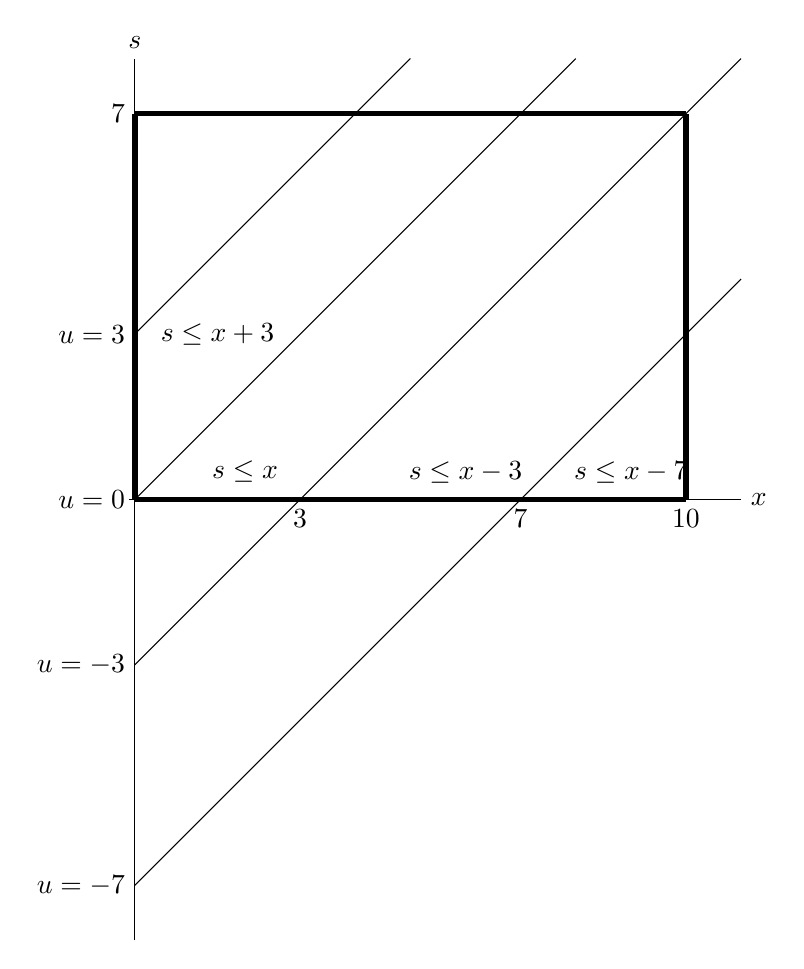
\begin{tikzpicture}[scale=0.7]
%\draw[[-{Triangle[open]},dotted] (0,10)--(8.5,10);
\draw (0,-8)--(0,8);
\node[right] at (11,0) {$x$};
\draw (-0.1,0)--(11,0);
\node[above] at (0,8) {$s$};
\draw[line width=0.7mm] (0,7)--(10,7);
\draw[line width=0.7mm] (10,0)--(10,7);
\draw[line width=0.7mm] (0,0)--(10,0);
\draw[line width=0.7mm] (0,0)--(0,7);
\node[below] at (10,0) {10};
\node[below] at (7,0) {7};
\node[below] at (3,0) {3};
\node[left] at (0,7) {7};
\draw (0,-7)--(11,4);
\node[left] at (0,-7) {$u=-7$};
\node at (9,0.5) {$s\leq x - 7$};
\draw (0,-3)--(11,8);
\node[left] at (0,-3) {$u=-3$};
\node at (6,0.5) {$s\leq x - 3$};
\draw (0,0)--(8,8);
\node[left] at (0,0) {$u=0$};
\node at (2,0.5) {$s\leq x$};
\draw (0,3)--(5,8);
\node[left] at (0,3) {$u=3$};
\node at (1.5,3) {$s\leq x+3$};
\end{tikzpicture}
\end{center}
%\caption{Computing the probability that $S-X\leq u$.}
%\label{fig:P_S_X}
%\end{figure}


It is clear that the indicated rectangle has no overlap with the set of points $(x,s)$ such that $s\leq u + x$ for $u<-10$. (To see this, draw the line $s=x-10$ in the figure.) At $u=-10$, the overlap is a single point, at $(10,0)$. Thus, 
\begin{equation*}
\P{S-X \leq u}=0, \quad \text{for } u\leq -10.
\end{equation*}

When $u\in[-10, -3]$ we need to integrate over the triangle that results from cutting the line $s=x+u$ with the rectangle. The area is 
\begin{equation*}
70\, \P{S-X \leq u}= \frac{(10+u)^2}2, \quad \text{for } -10 \leq u\leq -3,
\end{equation*}
where we multiply with $70$ to get the normalization right. 

When $u\in[-3, 0]$, we integrate over a parallelogram with base $3+u$ and height $7$ plus the triangle below the line $s=x-3$. The area is 
\begin{equation*}
70\, \P{S-X \leq u}= (3+u)7 + \frac{(10-3)^2}2=7u + \frac{91}2, \quad \text{for } -3 \leq u\leq 0.
\end{equation*}

For $u\in[0, 7]$, we integrate over the trapezoid that results from intersecting the set $\{(x,s) : x \leq s \leq s + u\}$ and the rectangle plus the parallelogram plus the triangle below the line $s=x-3$. The area is 
\begin{equation*}
70\, \P{S-X \leq u}= \frac{7^2}2 - \frac{(7-u)^2}{2} + 3\cdot 7 + \frac{49}2 = 7 u - \frac{u^2}2 + \frac{91}2, \quad \text{for } 0\leq u\leq 7.
\end{equation*}

Finally, for $u\geq 7$, the set $s\leq x+u$ covers the entire rectangle. Hence, 
\begin{equation*}
70\, \P{S-X \leq u}= 70, \quad \text{for } 7\leq u.
\end{equation*}

Given the amount of effort I had to put into getting this answer, I wanted to check it. So I went to Wolfram Alpha (which is a great site for symbolic computations), and typed this: 
\begin{verbatim}
\int_{0}^{10} \int_0^7 Boole[s<= x + u] ds dx,
\end{verbatim}
so, once you know \LaTeX\/ you can use Wolfram Alpha. Wolfram Alpha turned it to 
\begin{verbatim}
Integrate[Boole[s <= u + x], {x, 0, 10}, {s, 0, 7}]
\end{verbatim}
If you fill this in at Wolfram, you'll get the results that we obtained above in seconds, rather than in one hour or so (depending on your proficiency with carrying out integrals).
\end{solution}
\end{exercise}

The time job $k$ \emph{leaves the queue and moves to the server} is given by
\begin{equation*}
 \tilde A_k = A_k + W_{Q,k},
\end{equation*}
because a job can only move to the server after its arrival plus the time it needs to wait in queue.
Note that we here explicitly use the FIFO assumption.
Right after the job moves from the queue to the server, its service starts.
Thus,~$\tilde A_{k}$ is also the epoch at which the service of job~$k$ starts.

After completing its service, the job leaves the system.
Hence, the \recall{departure time of the system} is
\begin{equation*}
 D_k = \tilde A_{k} + S_k.
\end{equation*}
This in turn specifies the departure process $\{D(t)\}$ as
\begin{equation*}
 D(t) = \max\{k : D_k \leq t\} = \sum_{k=1}^\infty \1{D_k \leq t}.
\end{equation*}



The \recall{sojourn time}, or \emph{waiting time in the system}, $W_k$, is the time a job spends in the entire system.
With the above relations we see that
\begin{equation}
 W_k = D_k - A_k = \tilde A_{k} + S_k -A_k = W_{Q,k} + S_k,
\end{equation}
where each of these equations has its own interpretation. 


\begin{extra}
 Explain that the following recursion for~$W_k$ is valid:
\begin{align}
 \label{eq:59}
 W_{Q,k} &= [W_{k-1} - X_k]^+, &
 W_{k} &= W_{Q,k} + S_k = [W_{k-1} - X_k]^+ + S_k,
\end{align}
from which follows a recursion for $D_k$:
\begin{equation}
 D_k = A_k + W_k.
\end{equation}
\begin{solution}
  Suppose $k$ arrives right after job $k-1$.
  Then job $k$ has to wait until job $k-1$ leaves, in other words, the service of job $k$ can start only after job $k-1$ leaves.
  Consequently, in this case, $W_{Q,k}=W_{k-1$.
    If there is time $X_k$ between jobs $k$ and $k-1$, then job $k$ has to spend $X_k$ less in queue.
    This explains the first formula.
    The rest follows right away.
\end{solution}
\end{extra}


\begin{extra}
 Assume that $X_1=10$, $X_2=5$, $X_3=6$ and $S_1 = 17$, $S_2=20$ and $S_3=5$, compute the arrival times, waiting times in queue, the sojourn times and the departure times for these three customers.
\begin{hint}
 The intent of this exercise is to make you familiar with the notation.

 BTW, such simple test cases are also very useful to test computer code.
 The numbers in the exercise are one such simple case.
 You can check the results by hand; if the results of the simulator are different, there is a problem.
\end{hint}
\begin{solution} Let's feed it to the computer. Mind that in Python (just like in C, and so on), arrays start at index 0, not at index 1. 
\begin{pyconsole}
X = [0, 10, 5, 6] 
S = [0, 17, 20, 5]
A = [0, 0, 0, 0]
for i in range(1, len(X)):
 A[i] = A[i-1] + X[i]

A

WQ = [0, 0, 0, 0]
for i in range(1, len(X)):
 WQ[i] = max(WQ[i-1] + S[i-1] - X[i], 0)

WQ

ST = [0,0,0,0]
for i in range(1, len(X)):
 ST[i] = WQ[i] + S[i]

ST

D = [0, 0, 0, 0]
for i in range(1, len(X)):
 D[i] = A[i] + WQ[i] + S[i]

D
\end{pyconsole}
 
\end{solution}
\end{extra}



\begin{extra}\clabel{ex:25}
 Assume that $X_k = 10$ minutes and $S_k = 11$ minutes for all
 $k$, i.e., $X_k$ and $S_k$ are deterministic and constant. What
 are $\lambda$ and $\mu$? Compute $A_k$, $W_k$, $D_k$ as functions of $k$. Then find expressions for $A(t)$ and $D(t)$.
\begin{solution}
 $\lambda=6$ per hour, and $\mu=60/11$ per hour. Note that
 $\mu < \lambda$. $A_0 = 0$, $A_1=10$, $A_2=20$, and so on. Hence,
 $A_k = 10k$. $W_{Q,0} = 0$, $W_{Q,1} = \max\{0 + 0-10,0\} = 0$.
 $W_{Q,2} = \max\{0+11-10,0\} =1$.
 $W_{Q,3} = \max\{1+11-10,0\} =2$. Hence, $W_{Q,k} = k-1$ for
 $k\geq1$. Thus, $W_k = k-1+11 = k + 10$ for $k\geq1$, and
 $D_k = 10k + k+10 = 11k+10$. Note that $W_k$ increases linearly
 as a function of $k$. All in all, $A(t) = \lfloor t/10\rfloor$, and $D(t) = \lfloor (t-10)/11 \rfloor$.
\end{solution}
\end{extra}


\begin{extra}
 Suppose that $X_k\in\{1,3\}$ such that $\P{X_k=1}=\P{X_k=3}$ and
 $S_k\in\{1,2\}$ with $\P{S_k=1}=\P{S_k=2}$. If $W_{Q,0}=3$, what are
 the distributions of $W_{Q,1}$ and $W_{Q,2}$? 
\begin{hint}
Use~\cref{eq:59}.
\end{hint}
\begin{solution} First find the distribution of $Y_k:=S_{k-1}-X_k$ so that we can write
 $W_{Q,k}=[W_{Q,k-1}+Y_k]^+$. Use independence of $\{S_k\}$ and $\{X_k\}$:
\begin{align*}
 \P{Y_k=-2} &=\P{S_{k-1}-X_k=-2} = \P{S_{k-1}=1, X_k=3} = \P{S_{k-1}=1}\P{X_k=3} = \frac14.
\end{align*}
Dropping the dependence on $k$ for ease, we get
\begin{align*}
 \P{Y=-2} &=\P{S-X=-2} = \P{S=1, X=3} = \P{S=1}\P{X=3} = \frac14,\\
 \P{Y=-1} &=\P{S=2}\P{X=3} = \frac14,\\
 \P{Y=0} &=\P{S=1}\P{X=1} = \frac14,\\
 \P{Y=1} &=\P{S=2}\P{X=1} = \frac14.
\end{align*}
With this
 \begin{align*}
 \P{W_{Q,1} = 1} &=\P{W_{Q,0} + Y= 1} = \P{3 + Y =1} = \P{Y=-2} =\frac14,\\
 \P{W_{Q,1} = 2} &= \P{3 + Y =2} = \P{Y=-1} =\frac14,\\
 \P{W_{Q,1} = 3} &= \P{3 + Y = 3} = \P{Y=0} =\frac14,\\
 \P{W_{Q,1} = 4} &= \P{3 + Y = 4} = \P{Y=1} =\frac14.\\
 \end{align*}
And, then
 \begin{equation*}
 \begin{split}
 \P{W_{Q,2} = 1} 
&=\P{W_{Q,1} + Y = 1} = \sum_{i=1}^4 \P{W_{Q,1} + Y = 1\given W_{Q,1}=i}\P{W_{Q,1}=i}\\
&=\sum_{i=1}^4 \P{i + Y = 1\given W_{Q,1}=i}\frac14
=\sum_{i=1}^4 \P{Y = 1-i\given W_{Q,1}=i}\frac14\\
&=\frac14\sum_{i=1}^4 \P{Y = 1-i} = \frac14(\P{Y = 0} + \P{Y=-1} +\P{Y=-2}) = \frac{3}{16}.
 \end{split}
 \end{equation*}

\begin{comment}
Typing the solution becomes boring\ldots, let's use the computer\footnote{To run this code, you need to install the lea package. This is a very useful package to help you with all kinds of probability experiments.}.

\begin{pyconsole}
import lea

W = 3
S = lea.vals(1, 2)
S
X = lea.vals(1, 3)
X

# This is WQ1
W = lea.max_of(W + S - X, 0, fast=True)
W

# This is WQ2
W = lea.max_of(W + S - X, 0, fast=True)
W
\end{pyconsole}
Great! Our handiwork matches with the computer's results. 
\end{comment}

\end{solution}
\end{extra}



\begin{exercise}\clabel{ex:l-149} 
Explain the following recursions for a single server queue: 
\begin{equation}
 \label{eq:45}
 \begin{split}
 A_k &= A_{k-1} + X_k, \\
 D_k &= \max\{A_k, D_{k-1}\} + S_k,\\
 W_k &= D_k - A_k.
 \end{split}
\end{equation}

\begin{solution}
 Of course, the service of job $k$ cannot start before it arrives.
 Hence, it cannot leave before $A_k + S_k$.
 Therefore it must be that $D_k \geq A_k +S_k$.
 But the service of job $k$ can also not start before the previous job, i.e.
 job $k-1$, left the server.
 Thus job $k$ cannot start before $D_{k-1}$.
 To clarify it somewhat further, define $S_k'$ as the earliest start of job $k$.
 Then it must be that $S_k' = \max\{A_k, D_{k-1}\}$---don't confuse the earliest start $S_k'$ and the service time $S_k$---and $D_k = S_k' + S_k$.
\end{solution}
\end{exercise}

The \recall{virtual waiting time process} $\{V(t)\}$ is the amount of waiting that an arrival would see if it would arrive at time $t$.
To construct $\{V(t)\}$, we simply draw lines that start at points $(A_k, W_k)$ and have slope -1, unless the line hits the $x$-axis, in which case the virtual waiting time remains zero until the next arrival occurs.


\begin{exercise}\clabel{ex:l-150}
 Provide a specification of the virtual waiting time process $\{V(t)\}$ for
 all $t$.
\begin{hint}Make a plot of the function $A_{A(t)}-t$. What is the meaning of $V(A_{A(t)})?$ What is
$V(A_{A(t)}) + A_{A(t)}-t$?
\end{hint}
\begin{solution}
 There is a funny way to do this.
 Recall from a previous exercise that if $A(t)=n$, then $A_n$ is the arrival time of the $n$th job.
 Thus, the function $A_{A(t)}$ provides us with arrival times as a function of $t$.
 When $t=A_{A(t)}$, i.e., when $t$ is the arrival time of the $A(t)$th job, we set $V(t) = V(A_{A(t)}) = W_{A(t)}$, i.e., the virtual waiting time at the arrival time $t=A_{A(t)}$ is equal to the waiting time of the $A(t)$th job.
 Between arrival moments, the virtual waiting time decreases with slope $1$, until it hits 0.
 Thus,
 \begin{equation*}
 V(t) 
= [V(A_{A(t)}) - (t-A_{A(t)})]^+= [W_{A(t)} + (A_{A(t)}-t)]^+.
 \end{equation*}
 The notation may be a bit confusing, but it is in fact very simple.
 Take some $t$, look back at the last arrival time before time $t$, which is written as $A_{A(t)}$.
 (In computer code these times are easy to find.)
 Then draw a line with slope $-1$ from the waiting time that the last arrival saw.
\end{solution}
\end{exercise}

Once we have the arrival and departure processes it is easy to compute the \recall{number of jobs in the system} at time $t$ as, cf.~\cref{fig:atltdt},
\begin{equation}\label{eq:14}
 L(t) = A(t) - D(t) + L(0),
\end{equation}
where $L(0)$ is the number of jobs in the system at time $t=0$; typically we assume that $L(0)=0$.
As in a queueing system, jobs can be in queue or in service, we distinguish between the number in the system $L(t)$, the number in queue $L_Q(t)$, and the number of jobs in service $L_s(t)$.

\begin{extra}\clabel{ex:97}
In~\cref{ex:25},  find an expression for $L(A_k-)$. 
\begin{solution}
Recall that $A(t) = \lfloor t/10\rfloor$, and $D(t) = \lfloor (t-10)/11 \rfloor$.
  Hence,
 \begin{equation*}
 L(A_k-) = k-1 - D(A_k-) = k- 1 - D(10k-) = k- 1 - \left \lfloor \frac{(10k-)-10}{11} \right \rfloor.
 \end{equation*}
 The computation is a bit tricky since sometimes arrivals and departures coincide. (Consider for instance $t=120$.)

From this example you can infer that it is necessary that the service rate is greater than the arrival rate, i.e., $\mu > \lambda$, for otherwise, the queue length keeps on increasing (in the long run).
\end{solution}
\end{extra}

In summary, starting from a sequence of inter-arrival times $\{X_k\}$ and service times $\{S_k\}$ we can obtain a set of recursions by which we can simulate a queueing process in continuous time. A bit of experimentation with Python (or R perhaps) will reveal that this is easy.

\begin{extra}
 Explain that if we know $\tilde A(t)$, i.e.
 the number of jobs that departed from the queue up to time $t$, then
\begin{align*}
 L_Q(t) &= A(t) - \tilde A(t), \\
L_s(t) &= \tilde A(t) - D(t) = L(t) - L_Q(t).
\end{align*}
\begin{solution}
  We defined $\tilde A(t)$ as the amount of people up to time $t$ that left the queue and moved to the server.
  It is then clear to see that the number of jobs in queue $L_Q(t)$ is equal to the number amount of jobs that have arrived, i.e., $A(t)$, minus the number of jobs that left the queue, i.e., $\tilde A(t)$.
  Using the same reasoning for $L_s(t)$,  the second line also follows.
\end{solution}
\end{extra}



\begin{figure}[ht]
 \centering
\begin{tikzpicture}[scale=0.9,
 open/.style={shape=circle, fill=white, inner sep=1pt, draw, node contents=},
 closed/.style={shape=circle, fill=black, inner sep=1pt, draw, node contents=},
 soldot/.style={color=blue,only marks,mark=*}
]

\def\rightend{14}
\def\top{7}
\path [clip] (-1,-1) rectangle (\rightend,\top);

\draw[->] (-1,0) -- (\rightend,0);
\draw[->] (-0.5,-0.5) -- (-0.5, \top);

% arrivals
\def\lastx{0}
\foreach \x [count=\y, remember=\x as \lastx] in {1,3,4, 7, 9, 18} { 
 \node at (\lastx, 0) [below] {$A_{\y}$};
 \node (a) at (\lastx,\y) [closed] {};
 \draw[dotted] (\lastx,0) -- (a); 
 \draw (a)-- (\x,\y) node[open, label={}]; 
}
% draw first arrival. Since I want the circle to be open, I draw it at
% the end.
\node at (0, 0) [open] {};
\node at (5.5, 4) [fill=white] {$A(t)$};


% departures
\def\lastx{5}
\foreach \x [count=\y, remember=\x as \lastx] in {6, 8, 10, 11, 13,15} { 
 \draw[dotted] (\lastx,\y) -- (\lastx,0); 
 \draw (\lastx,\y) node[closed, label={}] -- (\x,\y) node[open, label={}]; 
 \node at (\lastx, -0.5) [below] {$D_{\y}$};
}
\node at (5, 0) [open] {};
\node at (12, 5) [fill=white] {$D(t)$};
 
\draw[dashed, <->] (3,2.5)--node[midway, fill=white] {$W_3$} (8,2.5);
\draw[dashed, <->] (7.5,2)--node[midway, fill=white,rotate=90] {$L(t)$} (7.5,5);

\end{tikzpicture}

 
\caption{Relation between the arrival process $\{A(t)\}$, the departure process $\{D(t)\}$, the number in the system $\{L(t)\}$ and the waiting times $\{W_k\}$.
 In particular, $L(t)$ is the difference between the graphs of $A(t)$ and $D(t)$.
}
 \label{fig:atltdt}
\end{figure}




\begin{extra}
 Why don't we need a separate notation for $D_s(t)$, the number of jobs that departed from the server?
\begin{solution}
 Because $D_s(t) = D(t)$. Once customers leave the server,
 their service is completed, and they leave the queueing system.
\end{solution}
\end{extra}

\begin{extra}
 Is $\tilde A(t) \leq D(t)$ or $\tilde A(t) \geq D(t)$?
\begin{solution}
 All customers that left the system must have left the
 queue. Thus, $\tilde A(t) \geq D(t)$.
\end{solution}
\end{extra}



\begin{extra}
 Consider a multi-server queue with $m$ servers.
 Suppose that at some time~$t$ it happens that $\tilde A(t) - D(t) < m$ even though $A(t) - D(t) > m$.
 How can this occur?
\begin{solution}
 In this case, there are servers idling while there are still
 customers in queue. If such events occur, we say that the server
 is not work-conservative.
\end{solution}
\end{extra}


\begin{exercise}\clabel{ex:l-151}
 Show that $L(t) = \sum_{k=1}^\infty \1{A_k \leq t < D_k}$ when the system starts empty.
\begin{hint}
 Use Boolean algebra.
 Write, for notational ease, $A=\1{A_k \leq t}$ and $\bar A = 1- A = \1{A_k > t}$, and define something similar for $D$.
 Then show that $A - D = A \bar D - \bar A D$, and show that $\bar A D =0$.
 Finally sum over $k$.
\end{hint}

\begin{solution}
 \begin{equation*}
 \begin{split}
 L(t)
&= A(t) - D(t) \\
&= \sum_{k=1}^\infty \1{A_k \leq t} - \sum_{k=1}^\infty \1{D_k \leq t} \\
&= \sum_{k=1}^\infty [\1{A_k \leq t} - \1{D_k \leq t}].
 \end{split}
 \end{equation*}
 Write for the moment $A=\1{A_k \leq t}$ and
 $\bar A = 1- A = \1{A_k > t}$, and likewise for $D$. Now we can use
 Boolean algebra to see that
 $\1{A_k \leq t} - \1{D_k \leq t} = A-D = A(D+\bar D) -D = AD +
 A\bar D - D = A\bar D - D(1-A) = A\bar D - D \bar A$.
 But $D \bar A = 0$ since
 $D \bar A = \1{D_k \leq t} \1{A_k > t} = \1{D_k \leq t < A_k}$
 which would mean that the arrival time $A_k$ of the $k$th job would
 be larger than its departure time $D_k$. As $A \bar D = \1{A_k \leq t < D_k}$
 \begin{equation*}
 \begin{split}
 L(t)
&= \sum_{k=1}^\infty [\1{A_k \leq t} - \1{D_k \leq t}] \\
&= \sum_{k=1}^\infty \1{A_k \leq t < D_k}.
 \end{split}
 \end{equation*}
 Boolean algebra is actually a really nice way to solve logical puzzles.
 If you are interested, you can find some examples on my homepage.
\end{solution}

\end{exercise}

\begin{extra} Show that $L(A_k)>0 \implies A_k \leq D_{k-1}$.
\begin{hint} Use that $L(A_k)>0$ means that the system contains at least one job at the time of the $k$th arrival, and that $A_k \leq D_{k-1}$ means that job $k$ arrives before job $k-1$ departs.
\end{hint}
\begin{solution} In a sense, the claim is evident, for, if the system contains a job when job $k$ arrives, it cannot be empty.
 But if it is not empty, then at least the last job that arrived before job $k$, i.e., job $k-1$, must still be in the system.
 That is, $D_{k-1} \geq A_k$.
 A more formal proof proceeds along the following lines.
 Using that $A(A_k) = k$ and $D(D_{k-1})= k-1$,
 \begin{equation*}
 \begin{split}
 L(A_k) &> 0 \Leftrightarrow A(A_k) - D(A_k) > 0 \Leftrightarrow k - D(A_k) > 0 \Leftrightarrow k > D(A_k) \\
 &\Leftrightarrow k-1 \geq D(A_k) \Leftrightarrow D(D_{k-1}) \geq D(A_k) \Leftrightarrow D_{k-1} \geq A_k, 
 \end{split}
 \end{equation*}
 where the last relation follows from the fact that $D(t)$ is a
 counting process, hence monotone non-decreasing.
\end{solution}
\end{extra}

Define the number of jobs in the system as seen by the $k$th arrival as
\begin{equation}
 \label{eq:Lk}
 L(A_k-).
\end{equation}
Observe that we write $A_k-$, and not $A_k$.
As we are concerned with a process with jumps, we need to be quite particular about left and right limits at jump epochs.


\begin{exercise}\clabel{ex:55}
  With the recursions~\cref{eq:59} it is apparently easy to compute the waiting time (in queue), but it is less simple to compute the number of jobs in queue or in the system.
  In this exercise we develop an algorithm to compute the number of jobs in the system as seen by arrivals.  Explain why the following (algorithmic efficient) procedure works: 
 \begin{equation*}
 L(A_k-) = L(A_{k-1}-)+1 - \sum_{i= k-1 - L(A_{k-1}-)}^{k-1} \1{D_i< A_k}.
 \end{equation*}
% \hint{ Realize that $L_k = k - 1 - D(A_k)$. 
% what happens to job k-1?
% }
\begin{solution}
 Let $ L(A_{k}-)$, i.e., the number of jobs in the system as
 `seen by' job $k$. It must be that $L(A_{k}-)=k-1 - D(A_{k})$. To see
 this, assume first that no job has departed when job $k$
 arrives. Then job $k$ must see $k-1$ jobs in the system. In general,
 if at time $A_k$ the number of departures is $D(A_k)$, then the
 above relation for $L(A_k-)$ must hold. Applying this to job $k-1$ we get that $L(A_{k-1}-) = k-2 - D(A_{k-1})$. 

 For the computation of $L(A_k-)$ we do not have to take the departures
 before $A_{k-1}$ into account as these have already been
 `incorporated in' $L(A_{k-1}-)$. Therefore,
 \begin{equation*}
 L(A_k-) = L(A_{k-1}-) + 1 - \sum_{i= k-1 - L(A_{k-1}-)}^{k-1} \1{D_i< A_k}.
 \end{equation*}

 Suppose $L(A_{k-1})=0$, i.e., job $k-1$ finds an empty system at its
 arrival and $D_{k-1}>A_{k}$, i.e., job $k-1$ is still in the
 system when job $k$ arrives. In this case, $L(A_{k}-)=1$, which checks
 with the formula. Also, if $L(A_{k-1}-)=0$ and $D_{k-1}< A_k$ then
 $L(A_k-) = 0$. This also checks with the formula. 

\end{solution}
\end{exercise}


\begin{extra}
 In~\cref{ex:55}, why do we take $i=k-1-L(A_{k-1}-)$ in the sum, and not $i=k-2-L(A_{k-1}-)$?
\begin{solution}
 The reason to start at $k-1-L(A_{k-1}-)$ is that the number in the
 system as seen by job $k$ is $k-1 - D(A_k)$ (not
 $k-2-D(A_k)$). Hence, the jobs with index from
 $k-1-L(A_{k-1}-), k-L(A_{k-1}-), \ldots, k-1$, could have left the system
 between the arrival of job $k-1$ and job $k$.
\end{solution}
\end{extra}




\begin{extra}[Not obligatory] Try to extend the recursions~\cref{eq:45} to a situation in which one queue is
 served by two servers. 
\begin{hint} The problem is
 that in a multi-server queueing systems, unlike for
 single-server queues, jobs can overtake each other: a small job
 that arrives after a very large job can still leave the system
 earlier. After trying for several hours, I obtained an inelegant
 method. A subsequent search on the web helped a lot. The
 solution below is a modification of N. Krivulin, `Recursive
 equations based models of queueing systems'. 
\end{hint}
\begin{solution}
The recursions for the two-server system are this: 
 \begin{equation*}
 \begin{split}
 A_k &= A_{k-1} + X_k, \\
 C_k &= \max\{A_k, D_{k-2}\} + S_k,\\
 M_k &= \max\{M_{k-1}, C_k\}, \\
 D_{k-1} &= \min\{M_{k-1}, C_k\}.
 \end{split}
 \end{equation*}
 Here, $C_k$ is the completion time of job $k$, and $\{D_k\}$ is
 a sorted list of departure times. Thus, $D_k$ is the $k$th
 departure time; recall this is not necessarily equal to the
 completion time $C_k$ of the $k$th job (as jobs may overtake
 each other). To understand the other equations, we reason like
 this. By construction, $C_k > D_{k-m}$ (as $S_k >0$).
 Therefore, when we arrived at time $C_k$, $(k-m)$ jobs must have
 departed. Moreover, by construction, $M_k$ tracks the latest
 completion time of all $k$ jobs, hence, $M_{k-m+1}$ is the latest
 completion time of the first $k-m+1$ jobs. Therefore, if
 $C_k>M_{k-1}$, job $k$ must leave later than the latest of the
 jobs in $\{1,2,\ldots, k-1\}$. Hence, the latest departure time
 of the jobs in $\{1, 2, \ldots, k-1\}$ jobs must be
 $M_{k-1}$. If however, $C_k<M_{k-1}$, then job $k$ leaves
 earlier than the latest of the jobs in $\{1,2,\ldots, k-1\}$. As
 $C_k>D_{k-2}$, it must be that $C_k > M_{k-2}$, because
 $D_{k-2}$ is the latest departure of the jobs in
 $\{1,2,\ldots, k-2\}$, and this is also equal to $M_{k-2}$. As a
 consequence, if $C_k < M_{k-1}$, job $k$ is also the first job
 that leaves after $D_{k-2}$ ( provided of course that
 $C_{k+1} < C_k$). Thus, all in all
 $D_{k-1} = \min\{M_{k-1}, C_k\}$.

In an attempt to extend the above to $m>2$ servers, I came up with this scheme:
 \begin{equation*}
 \begin{split}
 A_k &= A_{k-1} + X_k, \\
 C_k &= \max\{A_k, D_{k-m}\} + S_k,\\
 M_k &= \max\{M_{k-m+1}, C_k\}, \\
 D_{k-m+1} &= \min\{M_{k-m+1}, C_k\},
 \end{split}
 \end{equation*}
 but it is not correct. Can you find a counterexample?
\end{solution}
\end{extra}





\opt{solutionfiles}{
\Closesolutionfile{hint}
\Closesolutionfile{ans}
\subsection*{Hints}
\input{hint}
\subsection*{Solutions}
\input{ans}
}

%\clearpage

%%% Local Variables:
%%% mode: latex
%%% TeX-master: "../companion"
%%% End:

%%\section{Service Interruptions}
\section{Preemptive Interruptions, Server Failures}
\label{sec:preempt-interr-serv}


\opt{solutionfiles}{
\subsection*{Theory and Exercises}
\Opensolutionfile{hint}
\Opensolutionfile{ans}
}

%See section 1.11 of Zijm's book for the theory.

In~\cref{sec:setups-batch-proc,sec:non-preempt-interr} we assumed that servers are never interrupted while serving a job.
However, in many situations this assumption is not satisfied: a person might receive a short phone call while working on a job, a machine may fail in the midst of processing, and so on.
In this section we develop a model to compute the influence on the mean waiting time of such \emph{preemptive outages}, i.e., interruptions that occur \emph{during} a service.
As in~\cref{sec:non-preempt-interr}, to use the $G/G/1$ waiting time formula it suffices to find expressions for $\E S$ and $\V S$.
Thus, this will be our task for the rest of the section.
We remark in passing that the results and the derivation are of general interest.

Supposing that $N$ interruptions occur during the net service time $S_0$ of a job, the effective service time will be
\begin{equation*}
S= S_0 + \sum_{i=1}^N R_i.
\end{equation*}
A common assumption is that the time between two interruptions is $\Exp(\lambda_f)$, hence is memoryless.
Consequently, the number of interruptions $N$ that occur during the net service time $S_0$ is  Poisson distributed with mean $\E N = \lambda_f \E{S_0}$.
Define the \emph{availability} as
\begin{equation*}
  A=\frac{m_f}{m_f + m_r},
\end{equation*}
where $m_f$ is the mean time to fail and $m_r$ the mean time to repair. 
With this,
\begin{equation}\label{eq:83}
  \E S = \frac{\E{S_0}}{A}. 
\end{equation}
Finally, by  assuming that repair times are exponentially distributed with mean $\E{R}$, we can find that 
\begin{equation}\label{eq:87}
    C_s^2 = C_0^2 + 2 A(1-A) \frac{\E{R}}{\E{S_0}},
\end{equation}
where $C_0^2$ is the SCV of $S_0$, i.e., the service time without interruptions. 
It is important to realize that 
\begin{equation*}
\rho = \lambda \E S = \lambda \frac{\E{S_0}}A,
\end{equation*}
hence the server load increases due to failures. 

Before deriving the above expressions, let us see how to apply them. 

\begin{exercise}
  Suppose we have a machine with memoryless failure behavior, with a mean-time-to-fail of $3$ hours. Regular service times are deterministic with an average of 10 minutes, jobs arrive as a Poisson process with rate of 4 per hour.  Repair times are exponential with a mean duration of 30 minutes. What is the average sojourn time?
\begin{hint}
    Mind to work in a consistent set of units, e.g., hours. It is easy to make mistakes. 
\end{hint}
\begin{solution}
Let's first compute the load. If $\rho>1$ we are in trouble.
    \begin{pyconsole}
labda = 4.
ES0 = 10./60 # in hours
labda_f = 1./3
ER = 30./60 # in hours
A = 1./(1+labda_f*ER)
A
ES = ES0/A
ES
rho = labda*ES
rho
    \end{pyconsole}
As $\rho<1$, the system is not in overload. Now for the queueing time.
\begin{pyconsole}
Ca2 = 1.
C02 = 0. # deterministic service times
Ce2 = C02 + 2*A*(1-A)*ER/ES0
Ce2
EW = (Ca2+Ce2)/2 * rho/(1-rho) * ES
EW
EW + ES # sojourn time
\end{pyconsole}
\end{solution}
\end{exercise}

\begin{extra}
  Suppose we could buy another machine that never fails. What is the average sojourn time?
\begin{solution}
Now we don't need to take availability into account: the machine never fails so $A=1$. 
    \begin{pyconsole}
labda = 4.
ES0 = 10./60 # in hours
A = 1
ES = ES0/A
rho = labda*ES
rho
Ca2 = 1.
C02 = 0. # deterministic service times
EW = (Ca2+C02)/2 * rho/(1.-rho) * ES
EW
EW + ES # sojourn time
\end{pyconsole}
The average time in queue reduces from $\approx 0.6$ to $\approx 0.17$ hours, a reduction by about a factor 3. 
\end{solution}
\end{extra}

\begin{extra}\label{ex:79}
  Provide an intuitive explanation for $\E S = \E{S_0}/A$.
\begin{solution}
An intuitive way to obtain this result is by noting that $A$ is the fraction of time the server is working. As the total service time of a job is $\E S$, the net work done is $ A\E S$. But this must be the time needed to do the real job, hence $A \E S = \E{S_0}$.  
\end{solution}
\end{extra}


\begin{exercise}
  Show that $\E{S} = \E{S_0} + \E R \E N$; then show~\cref{eq:83}.
\begin{solution}
Write  $S_N = \sum_{i=1}^N R_i$ for the total duration of the interruptions, so that the total job duration becomes $S = S_0 + S_N$.    

\end{solution}
\end{exercise}


\begin{extra}\label{ex:84}
  Suppose that $N=n$, show that $\E{S_n}=n\E R$.
\begin{hint}
    Is it relevant  for the expectation of $S_n$ that $R_1,\ldots, R_n$ are mutually independent?
\end{hint}
\begin{solution}
The expectation of the sum of random variables is the same as the sum of the expectations; independence is irrelevant. Hence,
\begin{equation*}
  \E{S_n } =  \E{\sum_{i=1}^n R_i}=  n \E R, 
\end{equation*}
since by assumption $\E{R_1} = \cdots = \E{R_n}$. 
\end{solution}
\end{extra}


\begin{extra}\label{ex:16}
  Use~\cref{ex:84} to show that $\E{S_N}=\E R \E N$.
  This result is known as \recall{Wald's equation}.
\begin{hint}
  Use~\cref{eq:77}. 
\end{hint}
\begin{solution}
Since $\E{S_n} = n \E R$, 
\begin{align*}
  \E{\sum_{i=1}^N R_i} 
&=  \E{ \sum_{n=0}^\infty \1{N=n} \left(\sum_{i=1}^n R_i \right)} \\
&=  \sum_{n=0}^\infty \E{\1{N=n} n\E{R}} \\
&=  \E{R} \sum_{n=0}^\infty n \E{\1{N=n}} = \E R \sum_{n=0}^\infty n p_n\\
&= \E R \E N.
\end{align*}
\end{solution}
\end{extra}


\begin{extra}\label{ex:80}
  Show that  for our model of interruptions,
  \begin{equation*}
A=\frac 1{1+\lambda_f \E R}
  \end{equation*}
\begin{hint}
    Observe that $m_f = 1/\lambda_f$ and $m_r = \E R$.
\end{hint}
\begin{solution}
The time to fail is the time in between two interruptions. We assume that these times are $\Exp(1/\lambda_f)$. The duration of an interruption is $R$, which can be interpreted as the time to repair the server, hence $m_r = \E R$. With this
\begin{equation*}
  A=\frac{m_f}{m_f + m_r}=\frac{1/\lambda_f }{1/\lambda_f + \E R}. 
\end{equation*}
\end{solution}
\end{extra}


\begin{extra}
  Show that $\E{S} = \E{S_0} (1+\lambda_f \E R)$.
  Conclude that $\E S = \E{S_0}/A$.
\begin{hint}
    Realize that $\E N = \lambda_f \E{S_0}$. Then use~\cref{ex:80}.
\end{hint}
\begin{solution}
    \begin{equation*}
      \E S = \E{S_0} + \E N \E R = \E{S_0} +  \lambda_f \E{S_0} \E R= \E{S_0}(1+\lambda_f \E R).
    \end{equation*}
\end{solution}
\end{extra}


\begin{exercise}
  The derivation of $C_s^2$ is a bit more involved.
  To see this, explain that $\V{S} \neq \V{S_0} + \V{\sum_{i=0}^N R_i}$.
\begin{solution}
    Observe that $S_0$ and $N$ are not independent. In fact, when $S_0=s$, the number of failures $N$ is Poisson distributed with mean $\lambda_f s$. 
\end{solution}
\end{exercise}



\begin{extra}\label{ex:81}
Show that 
\begin{equation*}
  \E{S^2} = \E{S_0^2} + 2\E{S_0 \sum_{i=1}^N R_i} + \E{\sum_{i=1}^N R_i^2} + \E{\sum_{i=1}^N \sum_{j\neq i} R_i R_j}.
\end{equation*}
\begin{solution}
  Just work out the square of $S_0+\sum_{i=1}^N R_i$ and take expectations. Realize that $(\sum_i R_i)^2 = \sum_i R_i^2 + \sum_i\sum_{j\neq i} R_i R_j$.  
\end{solution}
\end{extra}


\begin{extra}
  To simplify the result of~\cref{ex:8}, we assume at first that $S_0$ is known, so that the number of failures that occur during a service time $S_0$ is Poisson distributed, i.e., $N\sim P(\lambda_f S_0)$.
  Show that $\E{S_0 \sum_{i=1}^N R_i\given S_0} = \lambda_f S_0^2 \E{R}$.
\begin{solution}
$\E{S_0 \sum_{i=1}^N R_i\given S_0} = 
S_0 \E{\sum_{i=1}^N R_i\given S_0} = S_0 \E R \E N = \lambda_f \E R S_0^2$.
\end{solution}
\end{extra}

\begin{extra} Now show that $\E{\sum_{i=1}^N R_i^2\given S_0} = \lambda_f S_0 \E{R^2}$.
\begin{hint}
  Use Wald's equation, which we derived in~\cref{ex:16}.
\end{hint}
\begin{solution}
  \begin{align*}
    \E{\sum_{i=1}^N R_i^2\given S_0} 
&= \E{R^2}\E{ \sum_{n=0}^\infty n \1{N=n}\given S_0}\\
&= \E{R^2} \E{N\given S_0} \\
&= \lambda_f S_0 \E{R^2}.
  \end{align*}
\end{solution}
\end{extra}

\begin{extra}
Show that 
$\E{\sum_{i=1}^N \sum_{j\neq i} R_i R_j\given S_0} = \lambda_f^2 S_0^2 (\E{R})^2.$
\begin{solution}
Since the $\{R_i\}$ are i.i.d., 
  \begin{equation*}
\E{\sum_{i=1}^N \sum_{j\neq i} R_i R_j\given S_0}
= \E{N(N-1)|S_0} (\E{R})^2 
= (\E{N^2|S_0}-\E{N\given S_0}) (\E{R})^2.
  \end{equation*}
Now $\E{N^2\given S_0}=\lambda_f^2 S_0^2 +\lambda_f S_0$ and $\E{N\given S_0} = \lambda_f S_0$.
\end{solution}
\end{extra}

\begin{extra}\label{ex:82}
  Combine the above to see that
    $\E{S^2\given S_0} = \frac{S_0^2}{A^2} + \lambda_f \E{R^2} S_0$. From this, 
  \begin{equation*}
    \E{S^2} = \frac{\E{S_0^2}}{A^2} + \lambda_f \E{R^2} \E{S_0}.
  \end{equation*}
\begin{solution}
For the first equation,
\begin{equation*}
  \E{S^2\given S_0} = S_0^2 + 2\lambda_f \E R S_0^2 + \lambda_f \E{R^2} S_0 + \lambda_f^2 (\E R)^2 S_0^2.
\end{equation*}
Assemble all terms with $S_0^2$ and observe that $(1/A) = 1+\lambda_f \E R$. For the second, recall that we assumed at first that $S_0$ was fixed, which we indicated by the condition on $S_0$. When $S_0$ is a random variable, we can just take the expectation at the left and right, and obtain the second result. 
\end{solution}
\end{extra}

\begin{extra}\label{ex:83}
Show that  
  \begin{equation*}
    \V{S} = \frac{\V{S_0}}{A^2} + \lambda_f \E{R^2} \E{S_0}.
  \end{equation*}
\begin{solution} 
    \begin{equation*}
    \V{S} = \E{S^2} - (\E S)^2 = 
\frac{\E{S_0^2}}{A^2} + \lambda_f \E{R^2} \E{S_0} -\frac{(\E{S_0})^2}{A^2}.
    \end{equation*}
\end{solution}
\end{extra}

\begin{exercise}
Show that
  \begin{equation*}
    C_s^2 = \frac{\V{S}}{(\E S)^2} = C_0^2 + \frac{\lambda_f \E{R^2} A^2}{\E{S_0}},
  \end{equation*}
\begin{hint} Just realize that $\E{S} = \E{S_0}/A$, and use the above.
\end{hint}
\begin{solution} Using~\cref{ex:81}--\cref{ex:83}
  \begin{align*}
C_s^2 &= \frac{\V{S}}{(\E S)^2} =\frac{V(S) A^2}{(\E{S_0})^2} \\
&=\frac{\E{S_0^2} + \lambda_f \E{R^2} \E{S_0}A^2 -(\E{S_0})^2}{(\E{S_0})^2} \\
&=\frac{\E{S_0^2} -(\E{S_0})^2}{(\E{S_0})^2} + \frac{\lambda_f \E{R^2} \E{S_0}A^2}{(\E{S_0})^2} \\
&=C_0^2 + \frac{\lambda_f \E{R^2}A^2}{\E{S_0}}.
  \end{align*}
\end{solution}
\end{exercise}


\begin{exercise}
With the above assumption on the distribution of $R$, show that
  \begin{equation*}
    C_s^2 = C_0^2 + 2 A(1-A) \frac{\E{R}}{\E{S_0}}.
  \end{equation*}

\begin{solution} 
When repair times are exponentially distributed with mean $\E{R}$:  $\E{R^2}=2(\E R)^2$. 

Since $A=1/(1+\lambda_f \E R)$, 
  \begin{equation*}
    \begin{split}
    \lambda_f \E{R^2} A^2 
&= 2\lambda_f (\E R)^2 A^2 = 2 \lambda_f \E R A A \E R \\
&= 2 \frac{\lambda_f \E R }{1+\lambda_f \E R} A \E R \\
&= 2 \left(1-\frac{1}{1+\lambda_f \E R}\right) A \E R  = 2(1-A)A \E R.
    \end{split}
  \end{equation*}
\end{solution}
\end{exercise}



\opt{solutionfiles}{
\Closesolutionfile{hint}
\Closesolutionfile{ans}
\subsection*{Hints}
\input{hint}
\subsection*{Solutions}
\input{ans}
}


%\clearpage


%%% Local Variables:
%%% mode: latex
%%% TeX-master: "../companion"
%%% End:

%\section{Non-preemptive Interruptions, Server Adjustments}
\label{sec:non-preempt-interr}


In~\cref{sec:setups-batch-proc} we studied the effect of setup times between job batches with a fixed size~$B$.
%In other words, there are no setups between any two jobs, setups are \emph{planned} between $B$ jobs.
However, other types of interruptions can occur, such as a machine requiring random adjustments that can occur between any two jobs.
This type of outages is \recall{non-preemptive} as the outages do not interrupt the processing of a job in service.
In this section we develop a simple model to understand the impact of such outages on job sojourn times; we use the same notation as in~\cref{sec:setups-batch-proc} and follow the same line of reasoning.

\opt{solutionfiles}{
\subsection*{Theory and Exercises}
\Opensolutionfile{hint}
\Opensolutionfile{ans}
}

%See section 1.11 of Zijm's book for the theory.


We assume that adjustments $\{R_i\}$ occur geometrically distributed between any two jobs with a mean of $B$ jobs between any two adjustments.
Consequently, the probability of an outage between any two jobs is $p=1/B$.
Observe that geometrically distributed random variables satisfy the memoryless property in discrete time.
Hence, our assumption implies that the occurrence of an adjustment between jobs $i$ and $i+1$ has no effect on the probability that an adjustment is necessary between jobs $i+1$ and $i+2$.

With the model, we can obtain quantitative insights into the effects of reducing adjustment times or the variability of these adjustments times.
For instance, we might decide to do fewer adjustments, so that $p$ decreases, but at the expense of larger average outage times.
Thus, without needing to actually do the experiments in real life, we can evaluate the influence of such decisions.

Contrary to the batch processing case of~\cref{sec:setups-batch-proc}, we now only need to find the mean and variance of the effective processing times.
From~\cref{ex:l-256} and \cref{,ex:l-257} it follows that
\begin{exercise}\clabel{ex:l-256}
Show that the average effective processing time is given by
\begin{equation} \label{eq:88}
 \E{S} = \E{S_0} + \frac{\E R}B
\end{equation}

\begin{hint}
  If there is no interruption, the service time is $S_0$.
  However, if there is an interruption, the service of a job is $R + S_0$, since we add the outage time to the service time of the job.
  Relate this insight to~\cref{ex:49}.
  In that exercise, take $p=(B-1)/B$ as the probability of a short job of size $\E{S_0}$ and $q=1/B$ as the probability of a long job of $\E{S_0} + \E{R}$.
\end{hint}
\begin{solution}
 \begin{equation*}
 \E{S} = (1-p)\E{S_0} + p (\E{R} + \E{S_0}) = \E{S_0} \frac{B-1}B + (\E{S_0} + \E R) \frac 1B,
 \end{equation*}
since $p=1/B$. 
\end{solution}
\end{exercise}


%The next step is to compute $\E{S^2}$. 
\begin{extra}\clabel{ex:78}
 Show that
 \begin{equation*}
 \E{S^2} = \E{S_0^2} + 2\frac{\E{S_0}\E{R}} B + \frac{\E{R^2}}B.
 \end{equation*}
\begin{hint}
  Again, use~\cref{ex:49}.
\end{hint}
\begin{solution}
 \begin{align*}
 \E{S^2} 
&= (1-p) \E{S_0^2} + p \E{(S_0+R)^2}\\
&= (1-p) \E{S_0^2} + p \E{S_0^2} + 2 p \E{S_0} \E R + p \E{R^2}. 
 \end{align*}
 Simplify and substitute $p=1/B$. 
\end{solution}
\end{extra}

\begin{exercise}\clabel{ex:l-257}
Derive 
\begin{equation}\label{eq:89} 
 \V{S} = \V{S_0} + \frac{\V{R}} B + (B-1)\left(\frac{\E R}{B}\right)^2.
\end{equation}
\begin{hint}
 First compute $\E{S^2}$. See~\cref{ex:78}.
\end{hint}
\begin{solution}
 \begin{equation*}
 \begin{split}
\V{S} 
&=\E{S^2} - (\E{S})^2 \\
&= \E{S_0^2} + 2 \E{S_0} \E R\frac 1B + \E{R^2}\frac 1B \\
&\quad - (\E{S_0})^2 - 2\E{S_0}\E R \frac 1 B - (\E R)^2\frac1{B^2}\\
&= \V{S_0} + ((\E{R^2} - (\E R)^2)\frac 1 B + (\E R)^2\left(\frac 1B - \frac 1{B^2}\right).
 \end{split}
 \end{equation*}
\end{solution}
\end{exercise}


Thus, the effective server load including down-times is $\rho = \lambda \E{S}$, and we can compute the SCV of the effective job processing times.
With this, we have all elements to fill in the $G/G/1$ waiting time formula!


\begin{exercise}\clabel{ex:l-255}
 Jobs arrive as a Poisson process with rate $\lambda=9$ per working day.
 The machine works two $8$ hour shifts a day.
 Work not processed on a day is carried over to the next day.
 Job service times are 1.5 hours, on average, with standard deviation of $0.5$ hours.
 Outages occur on average between $30$ jobs.
The average duration of an outage  is of $5$ hours and has a standard deviation of $2$ hours.

 Compute the average waiting time in queue.
\begin{hint}
 Get the units right. First compute the load, and then compute the rest.
\end{hint}
\begin{solution}
 First we determine the load. 
 \begin{pyconsole}
B=30
ES0 = 1.5
labda = 9./(2*8) # arrival rate per hour
ER=5.
ESe=ES0+ER/B
ESe
rho = labda*ESe
rho
 \end{pyconsole}
So, at least the system is stable.

\begin{pyconsole}
VS0 = 0.5*0.5
VR = 2.*2.
VSe = VS0 + VR/B + (B-1)*(ER/B)**2
VSe
Ce2 = VSe/(ESe*ESe)
Ce2
\end{pyconsole}

And now we can fill in the waiting time formula.
\begin{pyconsole}
Ca2=1 # Poisson arrivals
EW = (Ca2+Ce2)/2 * rho/(1-rho) * ESe
EW 
\end{pyconsole}
\end{solution}
\end{exercise}


\begin{remark}
  Let us compare the results of this section to those of~\cref{sec:non-preempt-interr}.
  In both cases the expected service time is the same: an amount $\E R/ B$ gets added to the net processing time $\E{S_0}$.
  However, the impact on the SCV is different.
  Unexpected interruptions must have a larger effect on variability than expected interruptions.

  In more general terms, we can use part of the model of~\cref{sec:setups-batch-proc} to analyze the effect of planned maintenance---do an adjustment after every $B$ jobs.
  In the model of this section, adjustments arrive completely unexpectedly.
  With these two models we can compare the influence on waiting times of doing planned adjustments more often (take $B$ a bit small), but remove the unexpected interruptions.
  Hence, we have another set of tools to compare different scenarios to organize production systems.
\end{remark}

\opt{solutionfiles}{
\Closesolutionfile{hint}
\Closesolutionfile{ans}
\subsection*{Hints}
\input{hint}
\subsection*{Solutions}
\input{ans}
}

%\clearpage

%%% Local Variables:
%%% mode: latex
%%% TeX-master: "../companion"
%%% End:

%\section{Setups and Batch Processing}
\label{sec:setups-batch-proc}

In some cases machines have to be setup before they can start producing items.
Consider, for instance, a machine that paints red and blue bikes.
When the machine requires a color change, it may be necessary to clean up the machine.
Another example is an oven that needs a temperature change when different item types require different production temperatures.
Service operations form another setting with setup times: when servers (personnel) have to move from one part of a building to another, the time spent moving cannot be spent on serving customers.
In all such cases, the setups consume a significant amount of time; in fact, setup times of an hour or longer are not uncommon.
Clearly, in such situations, it is necessary to produce in batches: a server processes a batch of jobs (or customers) of one type or at one location, then the server changes from type or location, starts serving a batch of another type or at another location.
Once done with one type, the server is setup again, and so on.
Here we focus on the effect of change-over, or setup, times on the average sojourn time of jobs.

First we make a model and provide a list of elements required to compute the expected sojourn time of an item, then we illustrate how to use these elements in a concrete case.

\opt{solutionfiles}{
\subsection*{Theory and Exercises}
\Opensolutionfile{hint}
\Opensolutionfile{ans}
}



Specifically, we analyze the following batch queueing situation.
There are two job families, e.g., red and blue, each served by the same single server.
Jobs arrive at rate $\lambda_r$ and $\lambda_b$, respectively, so that the arrival rate of jobs is $\lambda= \lambda_b+\lambda_r$.
Jobs of both types require an average \recall{net processing time} of $\E S_0$, provided the server is already setup for the correct job color.
The setup times $\{R_i\}$ are assumed to form an i.i.d.
sequence with common random variable $R$ and independent of $S_0$.
The sojourn time comprises the following steps.
First, jobs of each color are assembled into batches of size $B$, which we assume to be the same for both colors.
Once a batch is complete, the batch enters a queue (of batches).
After some time the batch reaches the head of the queue.
Then the machine performs a setup, and starts processing each job individually until the batch is complete.
Finally, once a job is finished, it can leave the system; as a consequence, it does not have to wait for other jobs in the same batch to form a new batch.




\begin{exercise}\clabel{ex:48}
  Show that the average time needed to form (or assemble) a batch is given by
\begin{equation}\label{eq:79}
 \E{W_r} = \frac{B-1}{2\lambda_r}.
\end{equation}
\begin{hint}
 Show that the total time to form a red batch is $(B-1)/\lambda_r$. 
\end{hint}
\begin{solution}
 Suppose a batch is just finished. The first job of a new batch needs to wait, on average, $B-1$ inter-arrival times until the batch is complete, the second $B-2$ inter-arrival times, and so on. The last job does not have to wait at all. Thus, the total time to form a batch is $(B-1)/\lambda_r$. 

An arbitrary job can be anywhere in the batch, hence the average time a job must wait until the batch is complete is half the total time. 
\end{solution}
\end{exercise}

Now that we have a batch of jobs, we need to estimate the average time a batch spends in queue.
For this we can use the $G/G/1$ waiting time formula, but we have to convert the effects of the setup times into job service times.
Define, to this end, the \recall{effective processing time} $\E S$ as the average time the server is occupied with processing a job from a batch including the setup time required to setup the batch.

\begin{exercise}\clabel{ex:488}
  Motivate that the effective processing time of an \emph{item} should be defined as
\begin{equation}\label{eq:81}
 \E{S} = \E{S_0} + \frac{\E{R}} B.
\end{equation}
\begin{hint}
 What fraction of the setup time $\E R$ `belongs' to one job?
\end{hint}
\begin{solution}
  The total service time spent on a batch of size $B$ is $B \E{S_0} + \E R$.
  The effective time per job is then the average, i.e., $(B \E{S_0}+\E R)/B$.
  Simplifying gives the answer.
\end{solution}
\end{exercise}

With the previous exercise, the load becomes
\begin{equation*}
\rho = \lambda \left(\E{S_0} + \frac{\E{R}}B\right).
\end{equation*}
There is another important way to look at the load, see the next exercise.

\begin{exercise}\clabel{ex:489}
Explain that the load can also be written as
\begin{equation*}
\rho = \lambda_B (B \E{S_0} + \E R),
\end{equation*}
where $\lambda_B=\lambda/B$ is the arrival rate of \emph{batches} and $\E{S_B} = B \E{S_0} + \E R$ is the service time an entire batch.
\begin{solution}
It is evident that the rate at which batches arrive is 
\begin{equation*}
 \lambda_B = \frac \lambda B,
\end{equation*}
since both job colors have the same batch size. 
Then the equality has the interpretation of the batch arrival rate times the work per batch.
\end{solution}
\end{exercise}

\begin{exercise}\clabel{ex:l-137}
Show that the requirement $\rho < 1$ leads to the following constraint on the minimal batch size~$B$ 
 \begin{equation*}
 B>\frac{\lambda \E R}{1-\lambda \E{S_0}}.
 \end{equation*}
\begin{solution}
 We require that the load is less than one, in other words, that $\lambda\left(\E{S_0} + {\E{R}}/B\right) < 1$. This is equivalent to $\E{R}/B < 1/\lambda - \E{S_0}$, hence $B > \E{R}/(1/\lambda - \E{S_0})$. Multiplying with $\lambda$ gives the result. 
\end{solution}
\end{exercise}

Observe that we nearly have all elements to apply Sakasegawa's formula to the batch: the service time of a \emph{batch} is
\begin{equation}
  \label{eq:90}
\E{S_B} = \E R + B\E{S_0},
\end{equation}
and the load $\rho$ is given above.
Therefore it remains to find $C_{a,B}^2$ and $C_{s,B}^2$, for the \emph{batches, not the items}.

\begin{exercise}\clabel{ex:490}
Explain that the SCV of the batch inter-arrival times is given by
 \begin{equation}\label{eq:82}
C_{a,B}^2 = \frac{C_{a}^2}B.
\end{equation}
\begin{hint}
Use \cref{eq:95} and \cref{eq:94}.
\end{hint}
\begin{solution}
The variance of the inter-arrival time of batches is $B$ times the variance of job inter-arrival times. The inter-arrival times of batches is also $B$ times the inter-arrival times of jobs. Thus, 
\begin{equation*}
 C_{a,B}^2 = \frac{B \V{X}}{(B \E X)^2} = \frac{\V X}{(\E X)^2} \frac 1 B = \frac{C_a^2}{B}.
\end{equation*}
\end{solution}
\end{exercise}


\begin{exercise}\clabel{ex:491}
Show that the SCV $C_{s,B}^2$ of the service times of the batches takes the form
\begin{equation}\label{eq:84}
C_{s, B}^2 = \frac{B \V{S_0} + \V{R}}{(B \E{S_0} + \E R)^2}.
\end{equation}
\begin{hint}
 What is the variance of a batch service time?
\end{hint}
\begin{solution}
 The variance of a batch is $\V{\sum_{i=1}^B S_{0,i} + R} = B\V{S_0} + \V R$, since the normal service times $S_{0,i}, i=1,\ldots, B$ of the job are independent, and also independent of the setup time $R$ of the batch.
\end{solution}
\end{exercise}

Observe that we now have all elements to fill in Sakasegawa's formula, which becomes
\begin{equation*}
  \E{W_{Q,B}} = \frac{C_{a,B}^2 + C_{s,B}^2}2 \frac \rho{1-\rho} \E{S_B}.
\end{equation*}

It is left to find a rule to determine what happens to an item once the batch to which the item belongs enters service.
If the job has to wait until all jobs in the batch are served, the time an item spends at the server is $\E R + B \E{S_0}$.


\begin{exercise}\clabel{ex:492}
Show that, when items can leave right after being served, the time at the server is given by
\begin{equation}\label{eq:85}
\E{R} + \frac{B+1}{2}\E{S_0}.
\end{equation}
\begin{solution}
 First, wait until the setup is finished, then wait (on average) for half of the batch (minus the job itself) to be served, and then the job has to be served itself, that is,
$\E{R} + \frac{B-1}{2}\E{S_0} +\E{S_0}$.
\end{solution}
\end{exercise}


\begin{exercise}\clabel{ex:l-139}
 Jobs arrive at $\lambda=3$ per hour at a machine with $C_a^2=1$; service times are exponential with an average of 15 minutes. Assume $\lambda_r = 0.5$ per hour, hence $\lambda_b = 3-0.5=2.5$ per hour. Between any two batches, the machine requires a cleanup of 2 hours, with a standard deviation of $1$ hour, during which it is unavailable for service.
 What is the smallest batch size that can be allowed?

 What is the average time a red job spends in the system in case $B=30$ jobs?
 Finally, observe that there is $B$ that minimizes the average sojourn time.
\begin{solution}
First check the load.
\begin{pyconsole}
labda = 3 # per hour
ES0 = 15./60 # hour
ES0
ER = 2.
B = 30
ESe = ES0+ ER/B
ESe

rho = labda*ESe
rho
\end{pyconsole}
Evidently, the load is smaller than $1$. 

The minimal batch size is
\begin{pyconsole}
Bmin = labda*ER/(1-labda*ES0)
Bmin
\end{pyconsole}
So, with $B=30$ we are on the safe side. 

The time to form a red batch is 
\begin{pyconsole}
labda_r = 0.5
EW_r = (B-1)/(2*labda_r)
EW_r # in hours
\end{pyconsole}
And the time to form a blue batch is 
\begin{pyconsole}
labda_b = labda-labda_r
EW_b = (B-1)/(2*labda_b)
EW_b # in hours
\end{pyconsole}


Now the time a batch spends in queue
\begin{pyconsole}
Cae = 1.
CaB = Cae/B
CaB
Ce = 1 # SCV of service times
VS0 = Ce*ES0*ES0
VS0
VR = 1*1. # Var setups is sigma squared
VSe = B*VS0 + VR
VSe
ESb = B*ES0+ER
ESb
CeB = VSe/(ESb*ESb)
CeB
EWq = (CaB+CeB)/2 * rho/(1-rho) * ESb
EWq
\end{pyconsole}

The time to unpack the batch, i.e., the time at the server. 
\begin{pyconsole}
ES = ER + (B-1)/2 * ES0 + ES0 
ES
\end{pyconsole}


The overall time red jobs spend in the system.
\begin{pyconsole}
total = EW_r + EWq + ES
total
\end{pyconsole}

\end{solution}
\end{exercise}


\begin{exercise}\clabel{ex:l-138}
  What important insights can you learn from the above about setting proper batch sizes?
\begin{solution}
  We can derive a number of important insights from this model.
  First, the time to assemble and unpack batches increases linearly of $B$.
  Second, observe from~\cref{eq:82} and \cref{eq:84} that the SCVs are $B$ times as small, but in~\cref{eq:90} we see that the batch service time is roughly $B$ times larger.
  Thus, the factor $B$ approximately cancels out in Sakasegawa's formula.
  However, the load decreases as a function of $B$, and this is the most important reason to use batch production.
  Third, since the load decreases as a function of the $B$, the expected time in queue must also decrease.
  Combining this with the linear batch forming times, there must be a batch size that minimizes the total time in the system.
  Fourth, with a it of numerical experimentation will show that the minimum in the waiting time is rather insensitive to $B$.
  However, by making $B$ smaller, the load increases, and we know that queueing times increase very steeply when the load increases.
  Therefore, by making $B$ small, we `gain' time linearly in batch forming times, but we `pay' hyperbolically in $B$.
  Given the randomness in practical situations, it is better, when tuning the batch size to minimize the time in the system, to set $B$ a bit too large than too small.
\end{solution}
\end{exercise}

A much more interesting and realistic problem is to assume that we have many families such that items of family~$i$ arrive at rate $\lambda_i$ and require service time $S_i$.
Typically, the setup time depends on the sequence in which the families are produced; let this be given by $R_{ij}$ when the machine switched from producing family~$i$ to family~$j$.
Often, in practice, $R_{ij} \neq R_{ji}$, for example, a switch in color from white to black takes less cleaning time and cost than from black to white.
Then the problem becomes to determine a good schedule in which to produce the families and the batch size $B_i$, which may be depend on the family.
Here is an exercise to show how to handle a simple case.

\begin{exercise}\clabel{ex:l-254}
 Consider a paint factory that contains a paint mixing machine that serves two classes of jobs, A and B.
 The processing times of jobs of types A and B are constant and require $t_A$ and $t_B$ hours.
 The job arrival rate is $\lambda_A$ for type A and $\lambda_B$ for type $B$ jobs.
 It takes a setup time of $S$ hours to clean the mixing station when changing from paint type A to type B, and there is no time required to change from type B to A.

 To keep the system  stable, it is necessary to produce the jobs in batches, for otherwise the server, i.e., the mixing machine, spends a too large fraction of time on setups.
 Motivate that the following linear program can be used to determine the minimal batch sizes:
\begin{equation*}
 \text{minimize } T
\end{equation*}
such that $ T= k_A t_A + S + k_B t_B$, $\lambda_A T < k_A$ and $\lambda_B T < k_B$.
\begin{hint}
Here are some questions to help you interpret this formulation.
\begin{enumerate}
\item What are the decision variables for this problem? In other words, what are the `things' we can control/change?
\item What are the interpretations of $k_A t_A$, and $S+k_B t_B$?
\item What is the meaning of the first constraint? Realize that $T$
 represents one production cycle. After the completion of one such
 cycle, we start another cycle. Hence, the start of every cycle can
 be seen as a restart of the entire system.
\item What is the meaning of the other two constraints?
\item Why do we minimize the cycle time $T$?
\item Solve for $k_A$ and $k_B$ in terms of $S$, $\lambda_A, \lambda_B$ and $t_A, t_B$. 
\item Generalize this to $m$ job classes and such that the cleaning
 time between jobs of class $i$ and $j$ is given by $S_{i j}$. (Thus,
 the setup times are sequence-dependent.) 
\end{enumerate}
\end{hint}

\begin{solution}
 Realize that the machine works in cycles. A cycle starts with
 processing $k_A$ jobs of type A, then does a setup, and processes
 $k_B$ jobs of type B, and then a new cycle starts again. The time
 it takes to complete one such cycle is $T=k_A t_A + S + k_B t_B$.
 The number of jobs of type A processed during one such cycle is,
 of course, $k_A$. Observe next that the average number of jobs
 that arrive during one cycle is $\lambda_A T$. We of course want
 that $\lambda_A T< k_A$, i.e., fewer jobs of type A arrive on
 average per cycle than what we can process.
\end{solution}
\end{exercise}



\opt{solutionfiles}{
\Closesolutionfile{hint}
\Closesolutionfile{ans}
\subsection*{Hints}
\input{hint}
\subsection*{Solutions}
\input{ans}
}
%\clearpage

%%% Local Variables:
%%% mode: latex
%%% TeX-master: "../companion"
%%% End:

%\section{Queueing Processes as Regulated Random Walks}
\label{sec:queu-proc-as}

\subsection*{Theory and Exercises}

\Opensolutionfile{hint}
\Opensolutionfile{ans}



In the construction of queueing processes as set out in
Section~\ref{sec:constr-discr-time} we are given two sequences of
i.i.d. random variables: the number of arrivals $\{a_k\}$ per period
and the service capacities $\{c_k\}$. Assuming that jobs can be served
in the period they arrive, the departure and queue length processes
are generated by the recursions
\begin{equation}\label{eq:5}
  \begin{split}
  Q_k &= [Q_{k-1}+a_k - c_k]^+,\\
  d_k &= Q_{k-1} +a_k- Q_{k},
  \end{split}
\end{equation}
where $[x]^+ := \max\{x, 0\}$.  

\begin{exercise}\label{ex:24}
  Show that the scheme
  \begin{align*}
    d_k &= \min\{Q_{k-1}+a_k, c_k\}, \\
    Q_k &= Q_{k-1} + a_k - d_k,
  \end{align*}
  is equivalent to~\eqref{eq:5}. 
\begin{solution}
  \begin{align*}
    Q_k &= Q_{k-1} + a_k - d_k \\ 
        &= Q_{k-1} + a_k - \min\{Q_{k-1}+a_k, c_k\} \\
        &= \max\{Q_{k-1} + a_k - c_k, 0 \}.
  \end{align*}
\end{solution}
\end{exercise}


Observe now that the relation for $Q_k$ shares a resemblance to a random walk $\{Z_k, k=0,1,\ldots\}$ with  $Z_k$ given by
\begin{equation}\label{eq:44}
  Z_k = Z_{k-1} + a_k - c_k.
\end{equation}
To see that $\{Z_k\}$ is indeed a random walk, observe that $Z$ makes  jumps of size $a_k-c_k, k=1,\ldots$, and $\{a_k-c_k\}$ is a sequence of i.i.d. random variables since, by assumption,  $\{a_k\}$ and $\{c_k\}$ are i.i.d.

Clearly, $\{Z_k\}$ is `free', i.e., it can take positive and negative
values, but $\{Q_k\}$ is restricted to the non-negative integers.  In
this section we show how to build the queueing process $\{Q_k\}$ from
the random walk $\{Z_k\}$ using a device called a \emph{reflection map}, which gives an  elegant construction of a queueing process. Moreover, we can use the probabilistic
tools that have been developed for the random walk to analyze queueing
systems. One example is the distribution of the time until an
especially large queue length is reached; these times can be
formulated as \emph{hitting times} of the random walk. Another example
is the average time it takes to clear a large queue.

\begin{exercise}
Show that  $Q_k$ satisfies the relation
\begin{equation}\label{eq:reich1}
  Q_k = Z_k - \min_{1\leq i \leq k} Z_i\wedge 0,
\end{equation}
where $Z_k$ is defined by the above random walk and
we write $a\wedge b$ for $\min\{a,b\}$.
\begin{hint}
Note first that from the expression for $Z_k$,
  $a_k - c_k = Z_k - Z_{k-1}$. Use this to get
  $Q_k = [Q_{k-1} +Z_k- Z_{k-1}]^+$. Subtract $Z_k$ from both sides, use recursion and
  use subsequently,
\begin{align*}
&\max\{\max\{a,b\}, c\} = \max\{a,b,c\}, \\
&Q_0 = Z_0, \\
&\max\{-a, -b \} = -\min\{a,b\}.
\end{align*}
\end{hint}
\begin{solution}
Note first that from the expression
for $Z_k$, $a_k - c_k = Z_k - Z_{k-1}$. Using this in the recursion
for $Q_k$, we get
\begin{equation*}
  Q_k = [Q_{k-1} +Z_k- Z_{k-1}]^+,
\end{equation*}
thus, 
\begin{equation*}
  Q_k - Z_{k} = \max\{Q_{k-1} - Z_{k-1}, -Z_k\}.
\end{equation*}
From this, using recursion and the hints, we see that
\begin{equation*}
  \begin{split}
  Q_k - Z_{k} 
% &= \max\{Q_{k-1} - Z_{k-1}, -Z_k\} \\
&= \max\{\max\{Q_{k-2} - Z_{k-2}, -Z_{k-1}\}, -Z_k\} \\
&= \max\{Q_{k-2} - Z_{k-2}, -Z_{k-1}, -Z_k\} \\
&= \max\{Q_{0} - Z_{0}, -Z_1, \ldots, -Z_k\} \\
&= \max\{0, -Z_1, \ldots, -Z_k\} \\
&= - \min\{0, Z_1, \ldots, Z_k\}.
  \end{split}
  \end{equation*}
For further discussion, if you are interested, refer to
  \citet{baccelli88:_sampl_m_m}.
\end{solution}
\end{exercise}

This recursion for $Q_k$ leads to really interesting graphs. In Figure~\ref{fig:random_bernoulli}
 we take $a_k \sim B(0.3)$, i.e., $a_k$ is Bernoulli-distributed with success
parameter $p=0.3$, i.e., $\P{a_k = 1} = 0.3 = 1- \P{a_k=0}$, and
$c_k \sim B(0.4)$. In Figure~\ref{fig:random_walk},  $a_k\sim B(0.49)$ and
the random walk is constructed as
\begin{equation}\label{eq:51}
  Z_k = Z_{k-1} + 2 a_k -1.
\end{equation}
Thus, if $a_k=1$, the random walk increases by one step, while if $a_k=0$, the random walk decreases by one step, so that $Z_k \neq Z_{k-1}$  always. Observe that this is slightly different from a random walk that satisfies~\eqref{eq:44}; there, $Z_{k}=Z_{k-1}$, if $a_k=c_k$.


\begin{figure}[ht]
  \centering
% see progs/reflected_random_walk.py
\input{progs/reflected_bernoulli_walk.tex}
%\input{reflected_random_walk.tex}
\caption{The upper panel shows a graph of the random walk $Z$. An
  upward pointing triangle corresponds to an arrival, a downward
  triangle to a potential service. The lower panel shows the queueing
  process $\{Q_k\}$ as a random walk with reflection.}
\label{fig:random_bernoulli}
\end{figure}

\begin{figure}[ht]
  \centering
% see progs/reflected_random_walk.py
\input{progs/reflected_random_walk.tex}
\caption{Another example of a reflected random walk.}
\label{fig:random_walk}
\end{figure}


With~(\ref{eq:reich1}),  we see that a random walk $\{Z_k\}$ can be converted into a queueing
process $\{Q_k\}$, and we might try to understand the transient behavior of the latter by investigating the transient behavior of the former.  For this, we first relate the random walk of the type~\eqref{eq:51} to a random walk in continuous time. 

\begin{exercise}
  Let $N_{\lambda+\mu}$ be a Poisson process with rate $\lambda+\mu$. If $\{a_k\}$ is an i.i.d. sequence of Bernoulli random variables such that $\P{a_k=1} = \lambda/(\lambda+\mu)=1-\P{a_k=0}$, show that the random variable
  \begin{equation*}
    N_\lambda(t) = \sum_{k=1}^\infty a_k \1{k \leq N_{\lambda+\mu}(t)},
  \end{equation*}
has a Poisson distribution with rate $\lambda t$. 
\begin{hint}
Use Exercise~\ref{ex:1}.
\end{hint}
\begin{solution}
  From Exercise~\ref{ex:1} we know that thinning  a rate $\lambda$ Poisson process  with i.i.d. Bernoulli random variables with success probability $p$  leads to another Poisson process with rate $\lambda p$. In the present case, the original Poisson process has rate $\lambda+\mu$ and $p=\lambda/(\lambda+\mu)$. Hence, the random variable $N_{\lambda t}\sim P\left(\frac\lambda{\lambda+\mu} (\lambda+\mu)t\right) = P(\lambda t)$.
\end{solution}
\end{exercise}

Similarly, let
\begin{equation*}
  N_\mu(t) = N_{\lambda+\mu}(t) - N_\lambda(t) = \sum_{k=1}^\infty (1-a_k) \1{N_{\lambda+\mu}(t) \leq k};
\end{equation*}
but this is $N_{\lambda+\mu}(t)$ thinned by the Bernoulli random variables $\{1-a_k\}$. Let  $N_\lambda = \{N_\lambda(t)\}$ and $N_\mu = \{N_\mu(t)\}$  be the associated Poisson processes. 

With the processes $N_\lambda$ and $N_\mu$ constructed above from the sequence $\{a_k\}$ and the Poisson process $N_{\lambda+\mu}$ we can define the process $Z=\{Z(t)\}$ such that
\begin{equation*}
  Z(t) = Z(0)+N_\lambda(t) - N_\mu(t).
\end{equation*}
Thus, we let $N_\lambda$ correspond to job  arrivals and $N_\mu$ to departures. Observe that the times $\{T_k\}$ at which $Z$ makes jumps are such that $T_k-T_{k-1}$ have exponential distribution with mean $1/(\lambda+\mu)$. At the jump times, $Z(T_k) = Z_k$, where $Z_k$ satisfies~\eqref{eq:51} with $\P{a_k = 1} = \lambda/(\lambda+\mu)$.  We call $Z$ the \emph{free} $M/M/1$ queue as, contrary to the real $M/M/1$ queue, $Z$ can take negative values. 

\begin{exercise}  
Show that
\begin{equation*}
    \P{Z(t)=n}_m 
= e^{-(\lambda+\mu)t} \left(\frac\lambda\mu\right)^{(n-m)/2} \sum_{k=0}^\infty 
\frac{(t\sqrt{\lambda\mu} )^{2k+m-n}}{k!(k+m-n)!},
\end{equation*}
where $\P{\cdot}_m$ means that the random walk starts at $m$, i.e.,
$Z(0)=m$.

As an aside, the summation includes negative factorials when
$k+m-n<0$. The tacit assumption is to take $n!\in \{\pm \infty\}$ for
$n\in \Z_-$. Another way to get around this problem is to take
$k=\max\{0, m-n\}$.
\begin{hint}
It is actually not hard, even though the expression looks
  hard. Use conditioning to see that
  $\P{Z(t)=n}_m = \P{N_\mu(t) - N_\lambda(t) = m - n}$. Then write out
  the definitions of the two Poisson distributions. Assemble
  terms. Then fiddle a bit with the terms to get~$t\sqrt{\lambda\mu}$. 
\end{hint}
\begin{solution}
With this we have a characterization of the queue length process as a
function of time until it hits zero for the first time. What can we
say about the distribution of $Q(t)$? With the above random walk, 
\begin{equation}\label{eq:29}
  \begin{split}
    \P{Z(t)=n}_m
&= \P{m+N_\lambda(t) - N_\mu(t) = n }  = \P{N_\lambda(t) - N_\mu(t) = n-m }  \\
&= \P{N_\mu(t) - N_\lambda(t) = m-n }  \\
&= \sum_{k=0}^\infty \P{N_\mu(t) = k - n + m\given N_\lambda(t) = k } \P{N_\lambda(t)=k}\\
&= \sum_{k=0}^\infty e^{-\mu t} \frac{(\mu t)^{k -n+m}}{(k-n +m)!} e^{-\lambda t} \frac{(\lambda t)^k}{k!} \\
&= e^{-(\lambda+\mu)t} \sum_{k=0}^\infty \frac{(\lambda t)^k(\mu t)^{k  -n + m }}{k!(k-n+m)!}.
  \end{split}
\end{equation}
We can write this a bit simpler by noting that
\begin{align*}
  (\lambda t)^k (\mu t) ^{k + m - n}  
&=  \lambda^k t^k\mu^{k + m - n} t^{k+m-n} \\
&= \lambda^k \mu^{k + m - n} (t\sqrt{\lambda \mu})^{2k+m-n} (\lambda\mu)^{-k + (n-m)/2} \\
&= (\lambda/\mu)^{(n-m)/2} (t\sqrt{\lambda \mu})^{2k+m-n}.
\end{align*}
With this,
\begin{equation*}
    \P{Z(t)=n}_m 
= e^{-(\lambda+\mu)t} \left(\frac\lambda\mu\right)^{(n-m)/2} \sum_{k=0}^\infty 
\frac{(t\sqrt{\lambda\mu} )^{2k+m-n}}{k!(k+m-n)!}.
\end{equation*}
\end{solution}
\end{exercise}


The solution of the above exercise shows that there is no simple
function by which we can compute the transient distribution of 
this simple random walk $Z$. Since a queueing process is typically a
more complicated object (as we need to obtain $Q$ from $Z$ via~\eqref{eq:reich1}), our
hopes to finding anything simple for the transient analysis of the
$M/M/1$ queue should not be too high. And the $M/M/1$ is but the
simplest queueing system; other queueing systems will be more
complicated yet.  We therefore give up the analysis of such transient
queueing systems and we henceforth contend ourselves with the analysis
of queueing systems in the limit as $t\to\infty$.  This of course
warrants two questions: what type of limit is actually meant here, and
what is the rate of convergence to this limiting situation? We address
these questions subsequently.

The \emph{long-run limiting behavior} of a queueing system (i.e., the first question) is an
important topic by itself. The underlying question is what happens if
we simulate the system for a long time. For instance, does there exist
a random variable $Q$ such that $Q_k\to Q$ in some sense? The answer
to this question is in the affirmative, provided some simple stability
conditions are satisfied, see
Section~\ref{sec:rate-stability}. However, it requires a considerable
amount of mathematics to make this procedure precise. To sketch what
has to be done, first, we need to define $\{Q_k\}$ as random variables
in their own right. Note that up to now we just considered each $Q_k$
as a \emph{number}, i.e., a measurement or simulation of the queue
length time of the $k$th period. Defining $Q_k$ as a random variable
is not as simple as the definition of, for instance, the number of
arrivals $\{a_k\}$; these random variables can be safely
\emph{assumed} to be i.i.d. However, the queue lengths $\{Q_k\}$ are
certainly not i.i.d., but, as should be apparent from
Eq.~\eqref{eq:59}, they are \emph{constructed} in terms of
recursions. Next, based on these recursions, we need to show that the
sequence of distribution functions $\{G_k\}$ associated with the
random variables $\{Q_k\}$ converges to some limiting distribution
function~$G$, say. Finally, it is necessary to show that it is
possible to construct a random variable~$Q$ that has~$G$ as its
distribution function.  In this sense, then, we can say
that~$Q_k \to Q$. The random variable $Q$ is known as the
\recall{steady-state limit} of the sequence of random variables
$\{Q_k\}$, and the distribution $G$ of~$Q$ is known as the
\recall{limiting distribution} or \recall{stationary distribution} of $\{Q_k\}$.

In these notes we sidestep all these fundamental issues, as the
details require measure theory and more advanced probability theory
than we can deal with in this course. However, it can all be made
precise. 

We illustrate the rate of convergence to the limiting situation (i.e., the second question) by means of an example. Specifically, we consider the sequence of waiting times $\{W_{Q,k}\}$ to a limiting random variable $W_Q$, where $W_{Q,k}$ is constructed according to the recursion
Eq.~(\ref{eq:56}). Suppose that $X_k\sim U\{1,2,4\}$ and
$S_k\sim U\{1,2,3\}$.  Starting with $W_{Q,0}=5$ we use
Eq.~(\ref{eq:56}) to compute the \emph{exact} distribution of
$W_{Q,k}$ for $k=1,2,\ldots, 20$, c.f., the left panel in
Figure~\ref{fig:convergence}. We see that when $k=5$, the `hump' of
$\P{W_{Q,5}=x}$ around $x=5$ is due the starting value of
$W_{Q,0}=5$. However, for $k>10$ the distribution of $W_{Q,k}$ hardly
changes, at least not visually. Apparently, the convergence of the
sequence of distributions of $W_{Q,k}$ is rather fast. In the middle
panel we show the results of a set of \emph{simulations} for
increasing simulation length, up to $N=1000$ samples. Here the
\emph{empirical distribution} for the simulation is defined as
\begin{equation*}
\P{W_Q\leq x} =   \frac 1n \sum_{k=1}^n \1{W_{Q,k} \leq x},
\end{equation*}
where $W_{Q,k}$ is obtained by simulation. As should be clear from the
figure, the simulated distribution also seems to converge quite fast to
some limiting function. Finally, in the right hand panel we compare
the densities as obtained by the exact method and simulation with
$n=1000$. Clearly, for all practical purposes, these densities can be
treated as the same.

The combination of the fast convergence to the steady-state situation
and the difficulties with the transient analysis validates, to some
extent, that most queueing theory is concerned with the analysis of
the system in \emph{stationarity}. The study of queueing systems in
stationary state will occupy us for the rest of the book.

\begin{figure}
  \centering
% see progs/waiting_time_simulation.py
\input{progs/waiting_time_1.tex}
\input{progs/waiting_time_2.tex}
\input{progs/waiting_time_3.tex}
%  \includegraphics{progs/gg1convergence}
  \caption{The density of $W_{Q,k}$ for $k=5, 10, 15, 20$ computed by
    an exact method as compared the density obtained by simulation of
    different run lengths $N=200, 400, \ldots, 1000$. The right panel
    compares the exact density of $W_{Q,20}$ to the density obtained by simulation
    for $N=1000$.}
\label{fig:convergence}
\end{figure}




\begin{exercise}
  Suppose that $X_k\in\{1,3\}$ such that $\P{X_k=1}=\P{X_k=3}$ and
  $S_k\in\{1,2\}$ with $\P{S_k=1}=\P{S_k=2}$. Write a computer program
  to see how fast the distributions of $W_{Q,k}$ converge to a limiting distribution function.
  \begin{solution}
Here is an example with Python. In R it must be equally simple.
I compute the  difference, i.e., the Kolmogorov-Smirnov statistic, between
the distributions of $W_{Q,k-1}$ and $W_{Q,k}$, 
\begin{equation*}
  \max_x\{ |\P{W_{Q,k}\leq x} - \P{W_{Q,k-1}\leq x}|\},
\end{equation*}
for $x$ in the support of $W_{Q,k}$. 

The code can be found in the \pyv{exact} function in the file \pyv{waiting_time_simulation.py} at
    \href{https://github.com/ndvanforeest/queueing_book/tree/master/progs}{github}.

If you make a plot, you will see that after some 10 customers the distribution hardly changes any further. 

  \end{solution}
  \end{exercise}

\begin{exercise}
  Validate the results of  Figure~\ref{fig:convergence} with simulation.
  \begin{solution}
    The code is in the file \pyv{waiting_time_simulation.py} at
    \href{https://github.com/ndvanforeest/queueing_book/tree/master/progs}{github}.
\end{solution}
\end{exercise}

\Closesolutionfile{hint}
\Closesolutionfile{ans}

\opt{solutionfiles}{
\subsection*{Hints}
\input{hint}
\subsection*{Solutions}
\input{ans}
}
%\clearpage

%%% Local Variables:
%%% mode: latex
%%% TeX-master: "../queueing_book"
%%% End:

%\section{Rate, Stability and Load}
\label{sec:rate-stability}



In this section, we develop a number of essential concepts to analyze queueing systems: the arrival, service and departure rate.
With these we define the load, which is, arguably, the most important performance measure of a queueing system to check.
%We will use these concepts throughout the remainder of the book.

\opt{solutionfiles}{
\subsection*{Theory and Exercises}
\Opensolutionfile{hint}
\Opensolutionfile{ans}
}


We first formalize the arrival rate and departure rate in terms of the arrival and departure processes $\{A(t)\}$ and $\{D(t)\}$; recall that these are \emph{counting processes}.
The \recall{arrival rate} is the long-run average number of jobs that arrive per unit time along a sample path, i.e.,
\begin{equation}
 \label{eq:3}
 \lambda = \lim_{t\to\infty} \frac{A(t)}t.
\end{equation}
We remark in passing that this limit does not necessarily exist if $A(t)$ is some pathological function.
If, however, the inter-arrival times $\{X_k\}$ are the basic data, and $\{X_k\}$ are i.i.d.
and distributed as a generic random variable $X$ with finite mean $\E{X}$, we can construct $\{A_k\}$ and $\{A(t)\}$ as described in~\cref{sec:constr-gg1-queu}, and then the strong law of large numbers guarantees that the above limit exists.\footnote{In fact, $A(t)/t \to \lambda$ with probability one.}

\begin{extra}
  Can you make an arrival process such that $A(t)/t$ does not have a limit?
\begin{hint}
  As a start, the function $\sin(t)$ does not have a limit as $t\to\infty$.
  However, the time-average $\sin(t)/t \to 0$.
  Now you need to make some function whose time-average does not converge, hence it should grow fast, or fluctuate wilder and wilder.
\end{hint}
\begin{solution}
 If $A(t) = 3 t^2$, then clearly $A(t)/t = 3t$. This does not
 converge to a limit. 

 Another example, let the arrival rate $\lambda(t)$ be given as follows:
 \begin{equation*}
 \lambda(t) = 
 \begin{cases}
 1 & \text{if } 2^{2k} \leq t < 2^{2k+1} \\
 0 & \text{if } 2^{2k+1} \leq t < 2^{2(k+1)},
 \end{cases}
 \end{equation*}
 for $k=0,1,2,\ldots$.
 Let $A(t) = \lambda(t) t$.
 Then $A(t)/t$ does not have a limit.
 Of course, these examples are quite pathological, and are not representable for `real life cases'.
 (Although this is also quite vague.
 What, then, is a real-life case?)

 For the mathematically interested, we seek a function whose Ces\`aro limit does not exist.
\end{solution}
\end{extra}

Likewise, define the \recall{departure rate} as
\begin{equation}\label{eq:28}
 \delta = \lim_{t\to\infty} \frac{D(t)}t.
\end{equation}
Observe that, if the system is empty at time $0$, the number of departures must be smaller than or equal to the number of arrivals, i.e., $D(t) \leq A(t)$ for all $t$.
Therefore,
\begin{equation}\label{eq:26}
\delta = \lim_{t\to\infty} \frac{D(t)}t \leq \lim_{t\to\infty} \frac{A(t)}t = \lambda.
\end{equation}
It is evident that when $\lambda > \delta$, the system length process $L(t) \to \infty$ as $t\to \infty$.
We therefore call a system \recall{rate-stable} if
\begin{equation*}
 \lambda = \delta.
\end{equation*}
In  words: the system is rate-stable whenever jobs leave the system just as fast as they arrive in the long run.


\begin{exercise}\clabel{ex:98}
If the system starts empty, then we know that the number $L(t)$ in the system at time $t$ is equal to $A(t) - D(t)$.
Show that the system is rate-stable  if $L(t)$ remains finite, or, more generally, $L(t)/t \to 0$ as $t\to\infty$.
\begin{solution}
Since $L(t) = A(t) - D(t)$, 
\begin{equation*}
 \lambda = \lim_{t \to \infty} \frac{A(t)}t = \lim_{t \to \infty} \frac{D(t)+L(t)}t = \lim_{t \to \infty} \frac{D(t)}t + \lim_{t \to \infty} \frac{L(t)}t 
 = \delta. 
\end{equation*}
Hence, $\lambda=\delta$ when $L(t)/t\to0$.
\end{solution}
\end{exercise}


We next relate the arrival rate $\lambda$ to the expected inter-arrival time $\E X$.
Observe that at time $t=A_n$ precisely $n$ arrivals occurred.
Thus,
% by applying the definition of $A(t)$ at the epochs $A_n$,
we see that $A(A_n) = n$, and therefore
\begin{equation*}
 \frac{1}n\sum_{k=1}^n X_k = \frac{A_n}n = \frac{A_n}{A(A_n)}. 
\end{equation*}
But since $A_n\to\infty$ if $n\to\infty$, it follows from~\cref{eq:3} that the average inter-arrival time between two consecutive jobs is
\begin{equation}\label{eq:54}
 \E X = \lim_{n\to\infty} \frac{1}n\sum_{k=1}^n X_k = \lim_{n\to \infty} \frac{A_n}{A(A_n)} = \lim_{t\to\infty} \frac t{A(t)} = \frac 1 \lambda,
\end{equation}
where we take $t=A_n$ in the limit for $t\to\infty$.
In words, the arrival rate $\lambda$ is the \emph{inverse} of the expected inter-arrival time $\E X$.


Assume now that there is a single server.
Let $S_k$ be the required service time of the $k$th job to be served, so that  $U_n = \sum_{k=1}^n S_k$ becomes the total service time required by the first $n$ jobs.
With this, let $ U(t) = \max\{n: U_n \leq t\}$, so that we can define the \recall{service rate} or \recall{processing rate} as
\begin{equation*}
 \mu = \lim_{t\to\infty} \frac{U(t)}t.
\end{equation*}
Similar to the relation  $\E X= 1/\lambda$, we have the relation
\begin{equation*}
 \E S = \lim_{n\to\infty} \frac 1 n \sum_{k=1}^n S_k = \lim_{n\to\infty} \frac{U_n}{n} = \lim_{n\to\infty} \frac{U_n}{U(U_n)} = \lim_{t\to\infty} \frac t{U(t)} = \frac 1 \mu.
\end{equation*}
Thus,  the service rate $\mu$ is the \emph{inverse} of the expected service time $\E S$.

It turns out that, when $\mu = \lambda$ and $\V{S} > 0$ or $\V{X} >0$, the queue length process behaves in a very peculiar way.
This follows from the fact that the random walk without drift, i.e., $\mu=\lambda$, has some unexpected behavior\footnote{See any good book probability theory.}, and we know from~\cref{sec:queu-proc-as} that queueing system and random walks are intimately related.
To avoid such problems, we henceforth (and implicitly) require that $\mu > \lambda$.
Observe also the evident fact that jobs cannot depart faster than they can be served, hence, $D(t) \leq U(t)$ for all~$t$, hence $\delta \leq \mu$.
Combining this with $\lambda < \mu$ and rate-stability, we see that $\delta < \mu$.


\begin{extra}
  Define the random variables $\{\tilde X_k,k=1,\ldots\}$ as $\tilde X_k = S_{k-1}-X_k$.
  For stability of the queueing process it is essential that $\tilde X_k$ has negative expectation, i.e., $\E{\tilde X_k} = \E{S_{k-1}-X_k} < 0$.
  What is the conceptual meaning of this inequality?
\begin{solution}
 That the average time customers spend in service is smaller
 than the average time between the arrival of two subsequent
 jobs. 
\end{solution}
\end{extra}

\begin{exercise}\clabel{ex:l-253}
Define $\tilde X_k = S_{k-1}-X_k$.
 Show that $\E{\tilde X_k} <0$ implies that $\lambda<\mu$. 
\begin{hint}
Remember that $\{X_k\}$ and $\{S_k\}$ are sequences of i.i.d. random variables. What are the implications for the expectations?
\end{hint}
\begin{solution}
 $0> \E{\tilde X_k} = \E {S_{k-1}-X_k} = \E{ S_{k-1}}- \E {X_k} = \E S - \E X$, where we use the fact that the $\{S_k\}$ and $\{X_k\}$ are i.i.d. sequences. Hence, 
 \begin{equation*}
 \E X > \E S \iff \frac 1{\E S} > \frac1{\E X} \iff \mu > \lambda.
 \end{equation*}

\end{solution}
\end{exercise}

Perhaps the most important performance measure is the concept of \recall{load}~$\rho$, which is defined as the rate at which jobs arrive times the average amount of work per job: $\rho = \lambda \E S$.
From the identities $\lambda^{-1} = \E X$ and $\mu^{-1} = \E S$, we get some further relations:
\begin{equation}
 \rho = \lambda \E S = \frac{\lambda}{\mu} = \frac{\E S}{\E X}.
\end{equation}
Observe that by assumption $\mu> \lambda$, hence $\rho < 1$.
The relation $\rho=\E S/ \E X < 1$ then tells us that the average time it takes to serve a job must be less than the average time between two consecutive arrivals, i.e., $\E S < \E X$.
Also, when $\lambda < \mu$, it is easy to check with simulation that when $L(0)$ is very large, $L(t) \approx L(0) - (\mu-\lambda)t$ until the system is empty, while if $\lambda>\mu$, we have that $l(t) \approx L(0) + (\lambda-\mu)t$. 


\begin{exercise}\clabel{ex:l-164}
 Consider a queueing system with $c$ servers with identical production rates $\mu$.
 What would be a reasonable stability criterion for this system?
\begin{hint}
What is the rate in, and what is the service capacity?
\end{hint}
\begin{solution}
 The criterion is that $c$ must be such that $\lambda < c\mu$.
 (Thus, we interpret the number of servers as a \emph{control}, i.e., a `thing' we can change, while we assume that $\lambda$ and $\mu$ cannot be easily changed.)
 To see this, we can take two different points of view.
 Imagine that the $c$ servers are replaced by one server that works $c$ times as fast.
 The service capacity of these two systems (i.e., the system with $c$ servers and the system with one fast server) is the same, i.e., $c\mu$, where $\mu$ is the rate of one server.
 For the system with the fast server, the load is defined as $\rho =\lambda/c\mu$, and for stability we require $\rho<1$.
 Another way to see it is to assume that the stream of jobs is split into $c$ smaller streams, each with arrival rate $\lambda/c$.
 In this case, applying the condition that $(\lambda/c )/\mu<1$ per server leads to the same condition that $\lambda/(c\mu) < 1$.
\end{solution}
\end{exercise}


\begin{extra}[Not obligatory]
 In~\cref{eq:54} we replaced the limit with respect to $n$ by a limit with respect to~$t$.
 Use the notation $A_{A(t)}$ to show that this is allowed.
 Show next that the function $t\to A(t)$ as defined by~\cref{eq:2} is right-continuous.
\begin{hint}
 Use that $A_{A(t)} \leq t < A_{A(t)+1}$.
 Divide by $A(t)$ and take suitable limits.
 BTW, such type of proof is used quite often to show that the existence of one limit implies, and is implied by, the existence of another type of limit.
\end{hint}
\begin{solution}
 This exercise is meant to provide some insight into what needs to be done to put everything on solid ground.


 Observing that $A_{A(t)}$ is the arrival time of the last job before time $t$ and that $A_{A(t)+1}$ is the arrival time of the first job after time $t$:
 \begin{equation*}
 A_{A(t)} \leq t < A_{A(t)+1} \Leftrightarrow 
 \frac{A_{A(t)}} {A(t)} \leq \frac{t}{A(t)} <\frac{A_{A(t)+1}}{A(t)} = \frac{A_{A(t)+1}}{A(t)+1}\frac{A(t)+1}{A(t)}.
 \end{equation*}
 Now $A(t)$ is a counting process such that $A(t)\to\infty$ as $t\to\infty$.
 Therefore, $\lim_{t\to\infty} A_{A(t)}/A(t) = \lim_{n\to\infty} A_n/n$.
 Moreover, it is evident that $\lim_{t\to\infty} A_{A(t)+1}/(A(t)+1) = \lim_{t\to\infty} A_{A(t)}/A(t)$, and that $(A(t)+1)/A(t)\to 1$ as $t\to\infty$.
 Thus it follows from the above inequalities that $\lim_{n\to\infty} A_n/n = \lim_{t\to\infty} t/A(t)$.
 
 For the right-continuity of $A(t)$, define $f(t) = \1{A_1 \leq t}$.
 Observe first that $f(t)$ is increasing, and $f(t)\in\{0,1\}$.
 Thus, if $f(t)=1$ then $f(u)=1$ for all $u\geq t$, and if $f(t)=0$ then $f(u) = 0$ for all $u\leq t$.

 You may skip the rest of the proof below, but the above is essential to memorize; make a plot of $f(t)$, in particular, the behavior around $A_1$ is important.

 We need to prove, for right-continuity, that $f(u)\to f(t) $ as $u\downarrow t$.
 When $f(t)=1$, $f(u)=1$ for any $u>1$, by the definition of $f(x)$.
 When $f(t)=0$ we have to do a bit more work.
 Formally, we have to prove that, for fixed $t$ and for all $\epsilon > 0$, there is a $\delta>0$ such that $u\in(t, t+\delta) \Rightarrow |f(u) -f(t)| < \epsilon$.
 (Note the differences with the regular definition of continuity.)
 Since, by assumption, $t$ is such that $f(t)=0$, and $f\in\{0,1\}$ we need to show that $f(u)=0$ for $u\in(t, t+\delta)$.
 Now, clearly, $f(t)=0$ only if $t < A_1$.
 But, then for any $u\in(t, A_1)$, we have that $f(u) = 0$.
 Thus, taking $\delta = A_1 - t$ suffices.

 The next step is to observe that $A(t)$ is a sum of right-continuous functions whose steps do not overlap since by assumption $0<A_1 < A_2 < \cdots$.
 As $A$ is (almost surely) a finite sum of bounded, increasing and right-continuous functions, it is also right-continuous.

 If you like, you can try to prove this last step too. 

 Hopefully this problem, and its solution, clarifies that even such small details require attention.
 If we want to make some progress with respect to developing some queueing theory, we have to skip most of the proofs and mathematical problems; we simply don't have enough time in this course to be concerned with all theorems and proofs.

 % For finite sums it is simple. Suppose that $f$ and $g$ are
 % right-continuous, then
 % \begin{equation*}
 % |f(u) + g(u) - f(t) - g(t)| \leq |f(u)-f(t)|+|g(u)-g(t)|.
 % \end{equation*}
 % Since both terms at the right-hand side can be made arbitrarily
 % small, the left-hand side can also be made as small as we
 % like. With this we can see that the function
 % $F_N(t) = \sum_{n=1}^N f_n(x)$ is right-continuous if all $f_n$
 % are right-continuous, and also that $F_{N+1} = F_N + f_{N+1}$ is
 % right-continuous. As this applies for all $N$, it follows from
 % induction that $\lim_N F_N$ is right-continuous, provided this
 % limit exists. When $f_n$ are all increasing, which is the case for
 % our situation by taking $f_n(t) = 1\{A_n \leq t\}$, then this
 % limit certainly exists.
\end{solution}
\end{extra}


\opt{solutionfiles}{
\Closesolutionfile{hint}
\Closesolutionfile{ans}
\subsection*{Hints}
\input{hint}
\subsection*{Solutions}
\input{ans}
}
%\clearpage

%%% Local Variables:
%%% mode: latex
%%% TeX-master: t
%%% End:

%\section{Renewal Reward Theorem and load}
\label{sec:renew-reward-theor}

\opt{solutionfiles}{
\subsection*{Theory and Exercises}
\Opensolutionfile{hint}
\Opensolutionfile{ans}
}


We start with stating and proving (graphically) the \recall{renewal reward theorem}.
In the sequel, we will see many applications of this theorem.
In this section, we use it to relate the fraction of time the server is busy in a $G/G/1$ queue to the job arrival rate and the expected job service time.


The renewal reward theorem is very useful and states intuitively that when customers arrive at rate $\lambda$ and each customer pays an average amount $X$, then the system earns money at rate $Y=\lambda X$.
\Cref{fig:renewal} provides graphical motivation about why this theorem is true; \citet{el-taha98:_sampl_path_analy_queuein_system} gives a (simple) proof.

\begin{theorem}[Renewal Reward Theorem, $Y=\lambda X$]
 Consider epochs $\{T_k, k=0, 1, \ldots\}$ such that $0=T_0 < T_1 < \cdots$
 Let $N=\{N(t), t\geq 0\}$ be the associated counting process with $N(t) = \max\{k : T_k \leq t\}$.
 Let $\{Y(t), t\geq 0\}$ be a non-decreasing right-continuous (deterministic) process.
 Define $X_k = Y(T_k)-Y(T_{k-1})$.
 Suppose that $N(t)/t\to\lambda$ as $t\to\infty$, where $0<\lambda < \infty$.
 Then $Y(t)/t$ has a limit iff $n^{-1}\sum_{k=1}^n X_k$ has a limit, and then $Y=\lambda X$. In other words, 
 \begin{equation*}
 \lim_{t \to \infty} \frac{Y(t)}t=Y \iff \lim_{n \to \infty} \frac 1n\sum_{k=1}^n X_k = X, 
 \end{equation*}
and then $Y=\lambda X$. 
\end{theorem}


\begin{figure}[ht]
 \centering
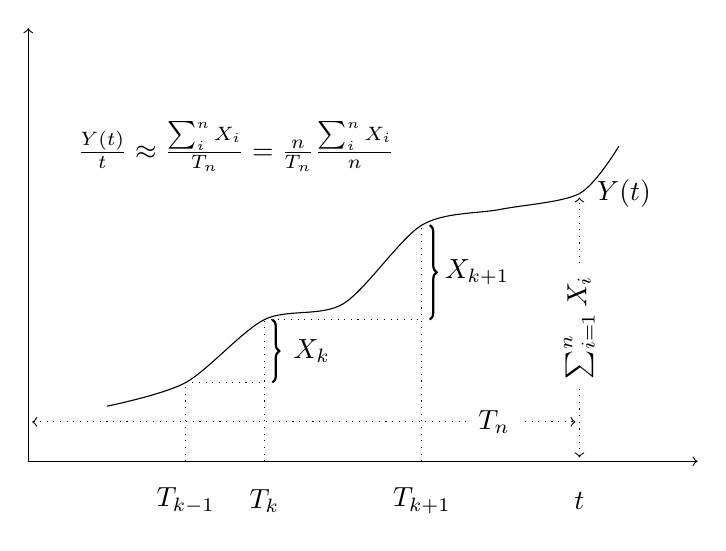
\begin{tikzpicture}[scale=1]
%axis
\draw[->] (0,0) -- coordinate (x axis mid) (8.5,0);
\draw[->] (0,0) -- coordinate (y axis mid) (0,5.5);
%\node[below=0.2cm] at (x axis mid) {$t$};

\draw plot [smooth] coordinates {(1,0.7) (2,1) (3,1.8) (4,2) (5,3) (6,3.2) (7, 3.4) (7.5,4.0)};
\node[right] at (7.1,3.4) {$Y(t)$};
\node at (7.,-0.5) {$t$};

\node at (2.,-0.5) {$T_{k-1}$};
\draw[dotted] (2,0)--(2,1);
\draw[dotted] (2,1)--(3,1);


\node at (3.,-0.5) {$T_{k}$};
\draw[dotted] (3,0)--(3,1.8);
\draw[dotted] (3,1.8)--(5,1.8);

\draw [
 thick,
 decoration={brace, mirror, raise=0.1cm },
 decorate
] (3,1) -- (3,1.8)
node[pos=0.5, xshift=0.6cm] {$X_k$}; 


\node at (5.,-0.5) {$T_{k+1}$};
\draw[dotted] (5,0)--(5,3);

\draw [
 thick,
 decoration={brace, mirror, raise=0.1cm },
 decorate
] (5,1.8) -- (5,3)
node[pos=0.5, xshift=0.7cm] {$X_{k+1}$}; 

\node[right] at (0.5,4) {$\frac{Y(t)}t \approx \frac{\sum_i^n X_i}{T_n} = \frac{n}{T_n} \frac{\sum_i^n X_i}n $};


\draw[dotted,<->, =stealth] (7,0.05)--(7,3.35) node[midway, rotate=90, fill=white] {$\sum_{i=1}^n X_i$};
\draw[dotted,<->, =stealth] (0.05,0.5)--(6.95,0.5) node[pos=0.85, fill=white] {$T_n$};
\end{tikzpicture}
\caption{A graphical `proof' of $Y=\lambda X$. Here $Y(t)/t\to Y$, $n/T_n\to \lambda$ and $n^{-1}\sum_i^n X_i \to X$. Observe that in the
 figure $X_k$ does not represent an inter-arrival time; instead it
 corresponds to the increment of (the graph of) $Y(t)$ between two
 consecutive epochs $T_{k-1}$ and $T_k$ at which $Y(t)$ is
 observed.}
 \label{fig:renewal}
\end{figure}

Define the \recall{load} or \recall{utilization} as the limiting fraction of time the server is busy, i.e.,
\begin{equation*}
 \rho = \lim_{t\to\infty} \frac 1 t \int_0^t \1{L(s)>0} \d s.
\end{equation*}

\begin{exercise}\clabel{ex:l-162}
Use the renewal reward theorem to prove that $\rho = \lambda \E S$ for the rate-stable $G/G/1$ queue. 
\begin{hint}
 Define $Y(t) = \int_0^t \1{L(s)>0} \d s$ as the total amount of time the server has been busy up to the time $t$.
 Then take as epochs $T_k = D_k$ and use rate stability.
\end{hint}
\begin{solution}
 It is evident that $X_k = Y(D_k)-Y(D_{k-1})=S_k$, hence $X = \lim_{n\to\infty} n^{-1}\sum_{k=1}^n X_k = \E S$.
 Also $\lim_{t\to\infty} Y(t)/t=\rho$.
 Finally, in the relation $Y = \lambda X$, the $\lambda$ is $\delta$ since we consider departure epochs $T_k = D_k$, rather than $A_k$.
 By the renewal reward theorem $Y=\lambda X$ we get that $\rho = \delta \E S$.
 Finally, by rate-stability, the job arrival rate $\lambda = \delta$, hence $\rho = \lambda \E S$.
\end{solution}
\end{exercise}


\begin{exercise}\clabel{ex:l-163}
 We can derive the relation $\rho = \lambda \E S$ in a somewhat more direct way by considering the fact that
\begin{equation*}
 \sum_{k=1}^{A(t)} S_k \geq \int_0^t \1{L(s)>0} \d s \geq \sum_{k=1}^{D(t)} S_k.
\end{equation*}
Explain this, and complete the argument.
\begin{solution}
Observe that
since $t$ can lie half way a service interval and $A(t) \geq D(t)$. As
$A(t)\to \infty$ as $t\to\infty$,
\begin{equation*}
 \lim_{t\to\infty} \frac 1 t\sum_{k=1}^{A(t)} S_k = 
 \lim_{t\to\infty} \frac{A(t)}t \frac{1}{A(t)} \sum_{k=1}^{A(t)} S_k = 
 \lim_{t\to\infty} \frac{A(t)}t \cdot \lim_{t\to\infty}\frac{1}{A(t)} \sum_{k=1}^{A(t)} S_k = \lambda \E S.
\end{equation*}
Applying similar limits to the other inequality gives
\begin{equation*}
\lambda \E S \geq \rho \geq \delta \E S.
\end{equation*}
Hence, if $\delta=\lambda$, $\rho = \lambda \E S$. 

Note that this is in fact the same argument as that underlies the renewal reward theorem. Henceforth we will just use the renewal reward theorem. 
\end{solution}
\end{exercise}


From the identities $\lambda^{-1} = \E X$ and $\mu^{-1} = \E S$, we get
a further set of relations:
\begin{equation*}
 \rho = \lambda \E S = \frac{\lambda}{\mu} = \frac{\E S}{\E X}.
\end{equation*}
Thus, the load has also the interpretation as the rate at which jobs
arrive times the average amount of work per job. Finally,
recall that for a system to be rate-stable, it is necessary that
$\mu> \lambda$, implying in turn that $\rho < 1$. The relation
$\rho=\E S/ \E X < 1$ then tells us that the average time it takes to
serve a job must be less than the average time between two consecutive
arrivals, i.e., $\E S < \E X$. In fact, when $\mu < \lambda$, it is easy to check with simulation that the queue length
grows roughly linearly with slope $\lambda - \mu$.


\begin{exercise}\clabel{ex:l-164}
 Consider a queueing system with $c$ servers with identical production rates $\mu$.
 What would be a reasonable stability criterion for this system?
\begin{hint}
What is the rate in, and what is the service capacity?
\end{hint}
\begin{solution}
 The criterion is that $c$ must be such that $\lambda < c\mu$.
 (Thus, we interpret the number of servers as a \emph{control}, i.e., a `thing' we can change, while we assume that $\lambda$ and $\mu$ cannot be easily changed.)
 To see this, we can take two different points of view.
 Imagine that the $c$ servers are replaced by one server that works $c$ times as fast.
 The service capacity of these two systems (i.e., the system with $c$ servers and the system with one fast server) is the same, i.e., $c\mu$, where $\mu$ is the rate of one server.
 For the system with the fast server, the load is defined as $\rho =\lambda/c\mu$, and for stability we require $\rho<1$.
 Another way to see it is to assume that the stream of jobs is split into $c$ smaller streams, each with arrival rate $\lambda/c$.
 In this case, applying the condition that $(\lambda/c )/\mu<1$ per server leads to the same condition that $\lambda/(c\mu) < 1$.
\end{solution}
\end{exercise}



\opt{solutionfiles}{
\Closesolutionfile{hint}
\Closesolutionfile{ans}
\subsection*{Hints}
\input{hint}
\subsection*{Solutions}
\input{ans}
}
%\clearpage


%%% Local Variables:
%%% mode: latex
%%% TeX-master: "../companion"
%%% End:

% \section{(Limits of) Empirical Performance Measures}
\label{sec:limits-of-emperical}


\subsection*{Theory and Exercises}

\Opensolutionfile{hint}
\Opensolutionfile{ans}

If the arrival and service processes are such that the queueing system
is rate-stable, we can sensibly define other performance measures such
as the average waiting time. In this section we define the second most
important performance measures; the most important being the
utilization $\rho$. We provide an overview of the relations between
these performance measures in Figure~\ref{fig:constructiongg1}.


With the construction of queueing processes in
Section~\ref{sec:constr-gg1-queu} we can compute the waiting time as
observed by the first $n$, say, jobs. Thus, the average waiting time
of the first $n$ arrivals is given by $n^{-1}\sum_{k=1}^n W_k$. We
therefore define the \recall{expected waiting time} as
\begin{equation}\label{eq:49}
  \E W = \lim_{n\to\infty} \frac 1n\sum_{k=1}^n W_k,
\end{equation}
and the expected time in queue as
\begin{equation}\label{eq:50}
  \E{W_Q} = \lim_{n\to\infty} \frac 1 n\sum_{k=1}^n W_{Q,k}.
\end{equation}
Note that these performance measures are limits of \emph{empirical}
measures.  Note also that these statistics are as \emph{observed by
  arriving jobs}: the first job has a waiting time $W_1$ at its
arrival epoch, the second a waiting time $W_2$, and so on. For this
reason we colloquially say that $\E W$ is the average waiting time as
`seen by arrivals'.  The \emph{distribution of the waiting times at
  arrival times} can be found by counting:
\begin{equation}\label{eq:48}
  \P{W \leq x}  = \lim_{n\to\infty} \frac 1n\sum_{k=1}^n \1{W_k\leq x}.
\end{equation}
Finally, the (sample) \recall{average number of jobs} in the system as seen by
arrivals is given by
\begin{equation}\label{eq:EQ}
\E L =  \lim_{n\to\infty}\frac 1 n \sum_{k=1}^n L(A_k-),
\end{equation}
where $L(A_k-)$ is the number of jobs in the system at the arrival epoch
of the $k$th job.  The \recall{distribution of $\{L(t)\}$ as seen by
  customers upon arrival}, is
\begin{equation}\label{eq:Qm}
\P{L\leq m} = \lim_{n\to\infty} \frac 1 n \sum_{k=1}^n \1{L(A_k-) \leq m}.
\end{equation}


\begin{exercise}
 Assume that $X_k = 10$ minutes and $S_k = 11$ minutes for all
    $k$, i.e., $X_k$ and $S_k$ are deterministic and constant. What
    are $\lambda$ and $\mu$?  Compute $A_k$, $W_k$ and $D_k$. 
    How do these numbers behave as a function of $k$?
  \begin{solution}
 $\lambda=6$ per hour, and $\mu=60/11$ per hour. Note that
      $\mu < \lambda$. $A_0 = 0$, $A_1=10$, $A_2=20$, etc., hence
      $A_k = 10k$. $W_{Q,0} = 0$, $W_{Q,1} = \max\{0 + 0-10,0\} = 0$.
      $W_{Q,2} = \max\{0+11-10,0\} =1$.
      $W_{Q,3} = \max\{1+11-10,0\} =2$. Hence, $W_{Q,k} = k-1$ for
      $k\geq1$. Thus, $W_k = k-1+11 = k + 10$ for $k\geq1$, and
      $D_k = 10k + k+10 = 11k+10$. Note that $W_k$ increases linearly
      as a function of $k$.  You can infer that, for the queue length
      to remain bounded, it is necessary that the service rate
      $\mu > \lambda$. 
  \end{solution}
\end{exercise}


\begin{exercise}
 Yet another simple case is to take $X_k=10$ minutes and
    $S_k=9$ minutes for all $k$. Answer the same questions as in the
    previous exercise.
  \begin{solution}
 Trivial.
  \end{solution}
\end{exercise}


A related set of performance measures follows by tracking the system's
behavior over time and taking the \emph{time-average}, rather than the
average at sampling (observation) moments. Thus, if we simulate the
queueing system up to time $t$, the \recall{time-average number of
jobs in the system} is given by
\begin{equation}\label{eq:11}
\frac 1 t\int_0^t L(s)\d s =  \frac 1 t\int_0^t (A(s)-D(s)) \d s,
\end{equation}
where we use that $L(s)=A(s) - D(s) + L(0)$ is the total number of jobs in
the system at time $s$ and $L(0)=0$, c.f. Figure~\ref{fig:atltdt}.  Observe from the second equation that $\int_0^t L(s)\d s$ is the area enclosed between the graphs of $\{A(t)\}$
and $\{D(t)\}$. Assuming the limit exists for $t\to\infty$, we define
\begin{equation}
  \label{eq:46}
  \E L = \lim_{t\to\infty} \frac 1 t\int_0^t L(s) \d s. 
\end{equation}
Observe that, notwithstanding that the symbols are the same, this
expectation need not be the same as~\eqref{eq:EQ}: in general,
\begin{equation*}
  \lim_{t\to\infty} \frac 1 t\int_0^t L(s)\, \d s \neq   \lim_{n\to\infty}\frac 1n  \sum_{k=1}^n L(A_k-).
\end{equation*}

\begin{exercise}
Design a queueing system to show that average number of jobs in the system as seen by the server is very different from what the customers see.
  \begin{hint}
Consider a queueing system with constant service and inter-arrival times.
  \end{hint}
\begin{solution}
  Take $X_k = 10$ and $S_k = 10-\epsilon$ for some tiny
  $\epsilon$. Then $L(t) = 1$ nearly all of the time. In fact,
  $\E L = 1-\epsilon/10$. However, $L(A_k-)=0$ for all $k$.
\end{solution}
\end{exercise}

Next, define the following probability as the
\emph{time-average fraction of time the system contains at most $m$
  jobs}:
\begin{equation}
  \label{eq:47}
  \P{L\leq m} =\lim_{t\to\infty} \frac 1 t\int_0^t \1{L(s)\leq m} \d s.
\end{equation}
Again, this probability need not be the same as what customers see
upon arrival.  

\begin{exercise}
Formulate a definition  for the  time-average of the waiting time.
\begin{solution}
  \begin{equation*}
    \E{W} = \lim_{t\to\infty} \frac1t \int_0^t W(s) \d s.
  \end{equation*}
\end{solution}
\end{exercise}



\begin{figure}[hp]
  \centering
  \begin{tikzpicture}[node distance = 2.5cm]
\tikzset{
    %Define standard arrow tip
    >=stealth',
    %Define style for boxes
    % Define arrow style
    pil/.style={
           ->,
           thick,
           shorten <=2pt,
           shorten >=2pt,}
}

% Define block styles
\tikzstyle{block} = [rectangle, draw,text centered, rounded corners, minimum height=3em]

    % nodes
    \node [block, fill=red!50] (X_k) {$\{X_k\}$};
    \node [block, right=2.5cm of  X_k,fill=red!50] (A_k) {$\{A_k\}$}
    edge[pil,bend left=45] node[below] {$X_k := A_k - A_{k-1}$} (X_k)
    edge[pil,<-, bend right=45] node[above] {$A_k := A_{k-1} + X_{k-1}$} (X_k); 
    \node [block, right=2.5cm of  A_k ] (A_t) {$\{A(t)\}$}
    edge[pil,bend left=45] node[below] {$A_k := \inf\{t: A(t)\geq k\}$} (A_k)
    edge[pil,<-, bend right=45] node[above] {$A(t) := \max\{k: A_k\leq t\}$} (A_k); 
    \node [block, below=2cm of  X_k ] (EX) {$\frac 1n \sum_{k=1}^n X_k \to \E X$}
    edge[pil, <-] (X_k);
    \node [block, below=2cm of  A_t ] (lambda) {$\frac{A(t)}t  \to \lambda$}
    edge[pil, <-] (A_t);
    \node [block, below=2cm of  A_k ] {$\E X = \lambda^{-1}$}
    edge[pil, <-] (EX)
    edge[pil, <-] (lambda);

    \node[below=1cm of lambda] (dummy) {}; 

    \node [block, below=1cm of EX, fill=red!50] (S_k) {$\{S_k\}$};
    \node [block, right=2.5cm of  S_k ] (U_k) {$\{U_k\}$}
    edge[pil,<->] (S_k);
    \node [block, right=2.5cm of  U_k ] (U_t) {$\{U(t)\}$}
    edge[pil,<->]  (U_k);
    \node [block, below=1cm of  S_k ] (ES) {$\frac 1n \sum_{k=1}^n S_k \to \E S$}
    edge[pil, <-] (S_k);
    \node [block, below=1cm of  U_t ] (mu) {$\frac{U(t)}t  \to \mu$}
    edge[pil, <-] (U_t);
    \node [block, below=1cm of  U_k ] {$\E S = \mu^{-1}$}
    edge[pil, <-] (ES)
    edge[pil, <-] (mu);

    \node [block, right=of dummy] {Stability:\newline $\lambda < \mu$}
edge[pil,bend right=25, <-] (lambda.east)
edge[pil,bend left=25, <-] (mu.east);

    \node[block, below=1cm of  ES, fill=red!50 ] (W_k) {$W_{k}=\max\{W_{k-1} - X_k,0\} +S_k$};
    %edge[pil, bend left=45,<-]  (X_k)
    %edge[pil, bend right=55,<-]  (S_k.west);
    \draw[->] (S_k.west) [out=180, in=110] to  (W_k.north west);
    \draw[->] (X_k.west) [out=230, in=110] to  (W_k.north west);
    \node[block, right=1cm of  W_k, fill=red!50 ] (D_k) {$D_{k}=A_k + W_{k}$} 
    edge[pil,bend right=25, <-]  (A_k)
    edge[pil,<-]  (W_k);
    \node[block, right=1cm of  D_k ] (D_t) {$D(t)=\max\{k: D_k\leq t\}$} 
    edge[pil, <-]  (D_k);

    \node[block, below=1cm of  W_k, fill=blue!40] (W) {$\frac1n\sum_{k=1}^n W_k \to \E W$} 
    edge[pil, <-]  (W_k);
    \node[block, below=1cm of  D_t] (Q_t) {$L(t) := A(t) - D(t)$} 
    edge[pil, <-]  (D_t);
    \draw[->] (A_t.east) [out=20, in = 40] to  (Q_t);
    %edge[pil, bend right=95, <-]  (A_t.north);

    \node[block, right=1cm of  D_t] (delta) {$\frac{D(t)}t \to \delta$} 
    edge[pil, <-]  (D_t);


    \node[block, below=1cm of  D_k, fill=blue!40] (L) {$\frac 1 t \int_0^t L(s)\,\d s \to \E L$} 
    edge[pil, <-]  (Q_t);
    % \node[block, below=1cm of  L] (Little) {$\E L = \lambda \E W$} 
    % edge[pil, <-]  (L)
    % edge[pil, <-]  (W);

    \node[block, right=1cm of  Q_t] (hoi) {$\delta \leq \lambda$} 
    edge[pil, <-]  (delta)
    edge[pil, bend right=10, <-]  (lambda)
    edge[pil, bend left = 30, <-]  node[below] {$L(t)>0$} (Q_t);

    \node[block, below=1cm of W, fill=blue!40] (PW) {$\frac 1n \sum_{k=1}^n \1{W_k \leq w} \to \P{W\leq w}$}
    edge[pil, <-] (W);

    \node[block, below=1cm of Q_t, fill=blue!40] (PL) {$\frac 1t \int_{0}^t \1{L(s) \leq l} \to \P{L\leq l}$}
    edge[pil, <-] (Q_t);

% \node[block, below=1cm of PW, fill=gray!40] (PM) {Performance measures};
% \node[block, below=1cm of PM, fill=gray!40] {$G/G/1$ Construction \& simulation};

    % \node[block, below=1cm of L, text width=2cm, fill=gray!40] (perf) {Performance measures}
    % edge[pil, ->] (L)
    % edge[pil, ->] (PL)
    % edge[pil, ->] (PW)
    % edge[pil, ->] (W);

  \end{tikzpicture}  

  \caption{Here we sketch the relations between the construction of
    the $G/G/1$ queue from the primary data, i.e., the inter-arrival
    times $\{X_k; k\geq 0\}$ and the service times $\{S_k; k\geq 0\}$,
    and different performance measures. 
% The performance measures are
%     shown in \protect\tikz \protect\node[fill=blue!40] {blue};, the
%     essential components for the construction of the $G/G/1$ are shown
%     in \protect\tikz \protect\node[fill=red!40] {red}.
} 
    \label{fig:constructiongg1}

\end{figure}



\begin{exercise}
  Consider a discrete-time model of a queueing system, as we developed
  in Section~\ref{sec:constr-discr-time}.  The average number of customers
  that \emph{see upon arrival} more than~$m$ customers in the system
  cannot be defined as~\eqref{eq:Qm}. Provide a better definition. 
  \begin{hint}
Why is \eqref{eq:Qm} not the same as the number of
  batches that see a queue length less than~$m$?
  \end{hint}
  \begin{solution} Since we deal with a system in discrete time, $L_k$
    is the queue length at the end of period~$k$. Thus,
    $\sum_{k=1}^n \1{L_k > m}$ counts the number of \emph{periods}
    that the queue is larger than $m$. This is of course not the same
    as the number of \emph{jobs} that see a queue larger than $m$;
    only when $a_k>0$ the customers in a batch would see a queue
    $L_k>m$. Thus,
    \begin{equation*}
      \sum_{k=1}^n \1{L_k > m} \1{a_k > 0},
    \end{equation*}
    counts the number of batches. 

    Next, by assumption, $a_k$ customers arrive during period $k$. The
    first of these customers sees a queue length of $L_{k-1} - d_k$,
    the second $L_{k-1}-d_k + 1$, and so on until the last customer
    who sees a queue length of $L_{k-1} - d_k + a_k -1 = L_k
    -1$.
    Thus, of all jobs the last sees the largest queue. Hence, if
    $L_k \leq m$, all customers of the batch see a queue less than
    $m$. If, however, $L_k > m$, then $L_k -m$ customers saw $m$ or
    more jobs in the system. Therefore, the fraction of arrivals that
    see a queue with $m$ or more jobs is equal to
\begin{equation*}
  \frac 1 {A(n)} \sum_{k=1}^n (L_k - m) \1{L_k > m} .
\end{equation*}
We could also define this a bit differently. Suppose that we don't
want to distinguish between jobs in a batch, but simply want to say
that if one job sees a long queue, all see a long queue. In that case,
\begin{equation*}
\frac 1{A(n)}\sum_{k=1}^n a_k \1{L_k > m}.
\end{equation*}
Thus, when jobs arrive in batches, the definition of loss fraction
requires some care; not all definitions need to measure the same.
  \end{solution}
\end{exercise}



\Closesolutionfile{hint}
\Closesolutionfile{ans}

\opt{solutionfiles}{
\subsection*{Hints}
\input{hint}
\subsection*{Solutions}
\input{ans}
}


%\clearpage
  



%%% Local Variables:
%%% mode: latex
%%% TeX-master: "../queueing_book"
%%% End:

%\section{Level-Crossing and Balance Equations}
\label{sec:level-cross-balance}


\subsection*{Theory and Exercises}

\Opensolutionfile{hint}
\Opensolutionfile{ans}


Consider a system at which customers arrive and depart in single
entities, such as customers in a shop or jobs at some machine.  If the
system starts empty, then we know that the number $L(t)$ is the system
at time $t$ is equal to $A(t) - D(t)$. To illustrate:

\begin{figure}[h]
  \centering
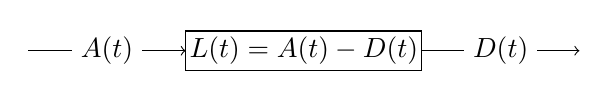
\begin{tikzpicture}[scale=1]
\draw[->] (0,0)--node[midway, fill=white] {$A(t)$}  (2,0); 
\draw (2,-0.25) rectangle node {$L(t)=A(t)-D(t)$} (5,0.25);
\draw[->] (5,0)--node[midway, fill=white] {$D(t)$}  (7,0); 
\end{tikzpicture}
\end{figure}

\noindent What goes in the box (i.e., $A(t)$) and has not yet left
  (i.e., $D(t)$) must still be in the box, hence $L(t)=A(t)-D(t)$). 



Let us denote an arrival as an `up-crossing' and a departure as a
`down-crossing'.  Then, clearly $L(t)$ is the number of up-crossings
up to time $t$ minus the number of down-crossings up to time $t$. If
$L(t)$ remains finite, or, more generally, $L(t)/t \to 0$ as $t\to\infty$, then it
must be that
\begin{equation*}
  \lambda =  \lim_{t \to \infty} \frac{A(t)}t  = \lim_{t \to \infty} \frac{D(t)+L(t)}t =  \lim_{t \to \infty} \frac{D(t)}t + \lim_{t \to \infty} \frac{L(t)}t 
  = \delta.  
\end{equation*}
Hence, when $L(t)/t\to0$, the \recall{up crossing rate}
$\lim_{t \to \infty} A(t)/t = \lambda$ is equal to the \emph{down-crossing rate}
$\lim_{t \to \infty} D(t)/t = \delta$.  We will generalize these notions of up- and
downcrossing in this section to derive the \recall{stationary}---also known as \emph{long-run time average} or \emph{steady-state},
distribution---$p(n)$ that the system contains $n$ jobs. 

\begin{exercise}
  If $L(t)/t \to 0$ as $t\to\infty$, can it still be true that $\E{L}>0$? 
  \begin{solution}
    \begin{equation*}
      \E{L} = \lim_{t\to\infty} \frac 1 t \int_0^t L(s) \d s \neq \lim_{t\to\infty} \frac{L(t)}t.
    \end{equation*}
If $L(t)=1$ for all $t$, $\E{L} =1 $, but $L(t)/t \to 0$. 
  \end{solution}
\end{exercise}


Let us say that the system is in \emph{state $n$ when it contains $n$
  jobs}, c.f. Figure~\ref{fig:A_n_t}, and the system \emph{crosses}
level $n$ when the state changes from $n$ to $n+1$, either `from
below' when an arrival occurs, or `from above' when a departure
occurs.  


\begin{figure}[th]
  \centering
\begin{tikzpicture}[scale=1,->,>=stealth',shorten >=1pt,auto,node distance=1.8cm,
                    semithick]
  \node[state] (0) {$p(0)$} ;
  \node[state] (1) [right of=0] {$p(1)$};
  \node[state] (2) [right of=1] {$p(2)$};
  \node[state] (3) [right of=2] {$p(3)$};
  \node[state] (4) [right of=3] {$\cdots$};

\path 
 (0) edge [bend left] node {$\lambda(0)$} (1)
 (1) edge [bend left] node {$\mu(1)$} (0)
 (1) edge [bend left] node {$\lambda(1)$} (2)
 (2) edge [bend left] node {$\mu(2)$} (1)
 (2) edge [bend left] node {$\lambda(2)$} (3)
 (3) edge [bend left] node {$\mu(3)$} (2)
 (3) edge [bend left] node {$\lambda(3)$} (4)
 (4) edge [bend left] node {$\mu(4)$} (3);

\draw[-, dotted, gray] (2.7,-2.)--(2.7,2.0) node[above, black] {level $1$};
\draw[->] (2,1.5)  node[left] {$A(1,t)$} -- (3.5,1.5);
\draw[<-] (2,-1.2) node[left] {$D(1,t)$} --(3.5,-1.2) ;

\end{tikzpicture}
\caption{ $A(1,t)$ counts the number of jobs up to time $t$ that saw 1
  job in the system; thus, right after the arrival of such a job the
  system contains 2 jobs. Similarly, $D(1,t)$ counts the number of
  departures that leave 1 job behind.  Each time $A(1,t)$ increases by
  one or $D(1,t)$ decreases by one, level $1$ (the dotted line
  separating states 1 and 2) is crossed.  The number of times this
  level is crossed from below must be the same (plus or minus 1) the
  number of times it is crossed from above. }
\label{fig:A_n_t}
\end{figure}



The main result we derive in this section is that the rate at
which level $n$ is crossed from below must match the rate at which it is crossed from above, i.e.,
\begin{equation*}
  \lambda(n) p(n) = \mu(n+1) p(n+1),
\end{equation*}
where $\lambda(n)$ is the arrival rate in state $n$, $p(n)$ the
fraction of time the system is in state $n$ and $\mu(n+1)$ the
departure rate from $n+1$. 

To establish this we need a few definitions
that are quite subtle and might seem a bit abstract, but below we will
provide intuitive interpretations in terms of system KPIs. Once we
have the proper definitions, the above result will follow
straightaway.


Define\footnote{It is common to write
  $f(x+) = \lim_{h\downarrow0} f(x+h)$ for the right limit of a
  function $f$ at $x$ and $f(x-) = \lim_{h\downarrow0} f(x-h)$ for the
  left limit. When $f(x-)=f(x+)$, $f$ is continuous at $x$. Since in
  queueing systems we are concerned with processes with jumps, we need
  to be quite particular about left and right limits at jump epochs.}
\begin{subequations}\label{eq:rates_}
\begin{equation}\label{eq:19} 
  A(n,t) = \sum_{k=1}^\infty \1{A_k \leq t}\1{L(A_k-) = n}
\end{equation}
as the number of arrivals up to time $t$ that saw $n$ customers in the system at their arrival.

\begin{exercise}
  Should we  take $L(A_k-)=n$ or $L(A_k)$ in the definition of $A(n,t)$?
  \begin{hint}
Recall that $L(t)$ is \emph{right-continuous}.
  \end{hint}
    \begin{solution}
    $L(t)$ is the number of customers in the system at time $t$. As
    such the function $t\to L(t)$ is \textsl{right-continuous}. The
    definition of $L(A_k-) = \lim_{t\uparrow A_k} L(t)$ is the
    limit from the left.  The customer therefore `sees' $L(A_k-)$ just
    before he/she arrives. 
\end{solution}  
\end{exercise}

\begin{exercise}
What is the difference between $A(n,t)$ and $A(t)$? 
\begin{solution}
  $A(t)$ counts all customers that arrive up to time $t$, i.e., during
  $[0,t]$. Note that this \textsl{includes} time $t$. $A(n,t)$ counts
  the jobs that see $n$ jobs in the system just before they arrive.
    \end{solution}
\end{exercise}

\begin{exercise}
 Show that $A(n,t) \leq A(t)$. 
\begin{solution}
       Observe that
      $\1{A_k\leq t}\1{L(A_k-) = n} \leq \1{A_k\leq t}$;
      the last inequality follows from the fact that
      $\1{L(A_k-) = n}\leq 1$. Therefore,
    \begin{equation*}
  A(n,t) = \sum_{k=1}^\infty \1{A_k \leq t} \1{L(A_k-) = n} 
\leq \sum_{k=1}^\infty \1{A_k \leq t} = A(t). 
    \end{equation*}
    For any `normal' queueing system, $A(t) > A(n,t)$, because the
    queue length fluctuates.
    \end{solution}
\end{exercise}



\begin{exercise}
  Why is $ \lim_{t\to\infty} \frac{A(n,t)}t = 0$ if
  $\lambda > \delta$, i.e., if the system is not rate-stable?
  \begin{solution}
 If $\lambda > \delta$, then $L(t)\to\infty$. But then there
      must be a last time, $s$ say, that $L(s) = n+1$, and $L(t) > n+1$
      for all $t>s$. Hence, after time $s$ no job will see the system
      with $n$ jobs. Thus $A(n,t) = A(n,s)$ for all $t>s$.  This is a
      finite number, while $t\to\infty$, so that $A(n,t)/t \to 0$.
  \end{solution}
 \end{exercise}


\begin{exercise}\label{ex:111}
  Consider the following (silly) queueing process. At times
  $0, 2,4, \ldots$ customers arrive, each customer requires $1$ unit
  of service, and there is one server. What acronym would describe this queueing situation? 
Find an expression for $A(n,t)$. 
  \begin{hint}
For the acronym, observe that the service times and
    inter-arrival are deterministic and there is one server. For
    the computation of $Y(n,t)$, make a plot of $L(s)$ as a
    function of time for $n=1$.

Make a plot of $L(s)$ for $n=1$ as a function of time. 
  \end{hint}
    \begin{solution}
      It is the $D/D/1$ queue, since there is one server and
      the inter-arrival times and service times are constant, i.e.,
      deterministic.


$A_k = 2k$ as jobs arrive at $t=0, 2, 4, \ldots$, hence,  $A(t) \approx t/2$ when $t\gg 0$. We also know that $L(s)=1$ if $s\in [2i, 2i+1)$ and $L(s)=0$ for $s\in[2i-1, 2i)$ for $i=0, 1, 2, \ldots$. Thus, $L(A_k-) = L(2k-)=0$. Hence, $A(0,t) \approx t/2$ for $t\gg 0$, and $A(n,t)=0$ for $n\geq 1$. 
    \end{solution}

\end{exercise}


Next, let 
\begin{equation} \label{eq:17} 
   Y(n,t) = \int_0^t  \1{L(s) = n} \d s
\end{equation}
be  the total time the system contains $n$ jobs during $[0,t]$, and
\begin{equation} \label{eq:18}
   p(n,t) = \frac 1 t \int_0^t  \1{L(s) = n} \d s = \frac{Y(n,t)}t,
\end{equation}
\end{subequations}
be the fraction of time that $L(s) =n$ in $[0,t]$. Figure~\ref{fig:Y_1_t} illustrates the relation between $Y(n,t)$ and $A(n,t)$.
  


\begin{exercise}\label{ex:112} Continuation of Exercise~\ref{ex:111}. 
Find an expression for $Y(n,t)$. 
    \begin{solution}
      Next, to get $Y(n,t)$, observe that the system never contains
      more than 1 job. Hence, $Y(n,t)=0$ for all $n\geq 2$.  Then we see that
      $Y(1,t) = \int_0^t \1{L(s) = 1}\d s.$ Now observe that for our
      queueing system $L(s)=1$ for $s\in[0,1)$, $L(s)=0$ for
      $s\in[1,2)$, $L(s)=1$ for $s\in[2,3)$, and so on, Thus, when
      $t<1$, $Y(1,t)=\int_0^t \1{L(s)=1} \d s = \int_0^t 1\d s = t$.
      When $t\in[1,2)$, 
      \begin{equation*}
        L(t)=0 \implies \1{L(t)=0} \implies Y(1,t) \text{ does not change}.
      \end{equation*}
Continuing to $[2,3)$ and so on gives
    \begin{equation*}
      Y(1,t) =
      \begin{cases}
        t & t\in[0,1), \\
        1 & t\in[1,2), \\
        1+(t-2) & t\in[2,3), \\
        2 & t\in[3,4), \\
        2+(t-4) & t\in[4,5), \\
      \end{cases}
    \end{equation*}
    and so on.  Since $Y(n,t)=0$ for all $n\geq 2$, $L(s) = 1$ or
    $L(s)=0$ for all $s$, therefore, 
    \begin{equation*}
      Y(0,t) = t-Y(1,t).
    \end{equation*}
    \end{solution}
\end{exercise}


\begin{figure}[t]
  \centering
\begin{tikzpicture}[scale=1,
  open/.style={shape=circle, fill=white, inner sep=1pt, draw, node contents=},
  closed/.style={shape=circle, fill=black, inner sep=1pt, draw, node contents=},
]

%axis
\draw[->] (0,0) -- coordinate (x axis mid) (8.5,0);
\draw[->] (0,0) -- coordinate (y axis mid) (0,4.5);
%\node[below=0.2cm] at (x axis mid) {$t$};
\node[left=0.3cm, rotate=90] at (y axis mid) {$L(t)$};


\draw 
node (0) at (0,0) [closed] {}
node (c1) at (1,0) [open] {};
\draw[thick] (0)--(c1);
\node[below] at (1,0) {$A_1$};

\draw 
node (c2) at (1,1) [closed] {}
node (c3) at (2.5,1) [open] {};
\draw[thick] (c2)--(c3);
\node[below] at (2.5,0) {$D_1$};

\draw 
node (c2) at (2.5,0) [closed] {}
node (c3) at (3,0) [open] {};
\draw[thick] (c2)--(c3);
\node[below] at (3,0) {$A_2$};

\draw 
node (c2) at (3,1) [closed] {}
node (c3) at (4,1) [open] {};
\draw[thick] (c2)--(c3);

\draw 
node (c2) at (4,2) [closed] {}
node (c3) at (5,2) [open] {};
\draw[thick] (c2)--(c3);
\node[below] at (4,0) {$A_3$};

\draw 
node (c2) at (5,1) [closed] {}
node (c3) at (5.8,1) [open] {};
\draw[thick] (c2)--(c3);
\node[below] at (5.,0) {$D_2$};

\draw 
node (c2) at (5.8,2) [closed] {}
node (c3) at (6.3,2)  {};
\draw[thick] (c2)--(c3);
\node[below] at (5.8,0) {$A_4$};

\draw[dashed] (1,0)--(2.5, 1.5) -- (3, 1.5)--(4,2.5) -- 
(5, 2.5)--(5.8, 3.3)--(6.3, 3.3);
\node[right] at (6.3, 3.3) {$Y(1,t)$};

\draw[dotted] (4,0) -- (4,0.5)--(5.8, 0.5)--(5.8, 1.5)--(6.3, 1.5);
\node[right] at (6.3, 1.5) {$A(1,t)$};

\end{tikzpicture}
  \caption{Plots of $Y(1,t)$ and $A(1,t)$. (For visual clarity, we subtracted $\nicefrac12$ from $A(1,t)$, for otherwise its graph would partly overlap with the graph of $L$.)}
  \label{fig:Y_1_t}
\end{figure}



Define also the limits:
\begin{align}\label{eq:p(n)}
  \lambda(n) &= \lim_{t\to\infty} \frac{A(n,t)}{Y(n,t)}, &p(n) &=\lim_{t\to\infty} p(n,t),
\end{align}
as the \emph{arrival rate in state $n$} and the \emph{long-run fraction of
  time the system spends in state $n$}. To clarify the former
definition, observe that $A(n,t)$ counts the number of arrivals that
see $n$ jobs in the system upon arrival, while $Y(n,t)$ tracks the amount of time
the system contains $n$ jobs. Suppose that at time~$T$ a job arrives that
sees $n$ in the system. Then $A(n,T)=A(n, T-)+1$, and this job finishes
an interval that is tracked by $Y(n,t)$, precisely because this job
sees $n$ in the system just prior to its arrival. Thus, just as
$A(t)/t$ is the total number of arrivals during $[0,t]$ divided by~$t$, $A(n,t)/Y(n,t)$ is the number of arrivals that see $n$ divided by
the time the system contains $n$ jobs.

\begin{exercise}\label{ex:113} Continuation of Exercises~\ref{ex:111} and~\ref{ex:112}.  Compute $p(n)$  and $\lambda(n)$. 
  \begin{solution}
    From the other exercises:
    \begin{align*}
      \lambda(0) &\approx \frac{A(0,t)}{Y(0,t)} \approx \frac{t/2}{t/2} = 1, \\
      \lambda(1) &\approx \frac{A(1,t)}{Y(1,t)} \approx \frac{0}{t/2} = 0, \\
      p(0) &\approx \frac{Y(0,t)}{t} \approx \frac{t/2}{t} = \frac 1 2, \\
      p(1) &\approx \frac{Y(1,t)}{t} \approx \frac{t/2}{t} = \frac 1 2.
    \end{align*}
For the rest $\lambda(n) = 0$, and $p(n)=0$, for $n\geq 2$.
  \end{solution}
\end{exercise}

Similar as the definition for $A(n,t)$, denote by
\begin{equation*}
    D(n,t) = \sum_{k} \1{D_k \leq t} \1{L(D_k) = n}
  \end{equation*}
  the number of departures up to time $t$ that\emph{ leave $n$
    customers behind}. Then,  define
\begin{equation*}
  \mu(n+1) = \lim_{t\to\infty} \frac{D(n,t)}{Y(n+1,t)},
\end{equation*}
as \emph{ the departure rate from state $n+1$}. (It is easy to get
confused here: to leave $n$ jobs behind, the system must contain $n+1$
jobs just prior to the departure.) Figure~\ref{fig:A_n_t} shows how
$A(n,t)$ and~$\lambda(n)$ relate to $D(n+1,t)$ and $\mu(n)$.

\begin{exercise}
Should  we take $D(n-1,t)$ or  $D(n,t)$ in the definition of $\mu(n)$?
    \begin{solution}
      $D(n-1,t)$ counts the departures that leave $n-1$ behind. Thus,
      just before the customer leaves, the system contains $n$
      customers.
\end{solution}
\end{exercise}

\begin{exercise}\label{ex:4}

Continuation of Exercises~\ref{ex:111},~\ref{ex:112}, and~\ref{ex:113}.  Compute 
$D(n,t)$ and $\mu(n+1)$ for $n\geq 0$.
\begin{solution}
  $D(0,t) = \sum_{k=1}^\infty\1{D_k\leq t, L(D_k)=0}$. From the graph of $\{L(s)\}$ we see that all jobs leave an empty system behind. Thus, $D(0,t) \approx t/2$, and $D(n,t)=0$ for $n\geq 1$. With this, $D(0,t)/Y(1,t) \sim (t/2)/(t/2) = 1$, and so,
  \begin{equation*}
    \mu(1) = \lim_t \frac{D(0,t)}{Y(1, t)} = 1,
  \end{equation*}
and $\mu(n) = 0$ for $n\geq2$. 
\end{solution}
\end{exercise}

Observe that customers arrive and depart as single units. Thus, if
$\{T_k\}$ is the ordered set of arrival and departure times of the
customers, then $L(T_k) = L(T_k-) \pm 1$. But then we must also have
that $|A(n,t) - D(n,t)| \leq 1$ (Think about this.). From this
observation it follows immediately that
\begin{equation}\label{eq:15}
  \lim_{t\to\infty} \frac{A(n,t)}t = \lim_{t\to\infty} \frac{D(n,t)}t.
\end{equation}
With this equation we can obtain two nice and fundamental
identities. The first we develop now; the second follows in
Section~\ref{sec:poisson-arrivals-see}.

The rate of jobs that `see the system with $n$ jobs' can be defined as
$A(n,t)/t$. Taking limits we get
\begin{subequations}
\label{eq:21}
\begin{equation}\label{eq:63}
  \frac{A(n,t)}t =   \frac{A(n,t)}{Y(n,t)}\frac{Y(n,t)}t \to \lambda(n) p(n),
\end{equation}
where we use the above definitions for $\lambda(n)$ and $p(n)$.
Similarly, the departure rate of jobs that leave $n$ jobs behind is
\begin{equation}\label{eq:22}
  \frac{D(n,t)}t =   \frac{D(n,t)}{Y(n+1,t)}\frac{Y(n+1,t)}t \to \mu(n+1) p(n+1).
\end{equation}
\end{subequations}
Combining this with~\eqref{eq:15} we arrive at \recall{the
  level-crossing equations}
\begin{equation}\label{eq:12}
  \lambda(n) p(n) = \mu(n+1)p(n+1).
\end{equation}

\begin{exercise} Continuation of Exercises~\ref{ex:111},~\ref{ex:112}, and~\ref{ex:113}.  Compute 
$\lambda(n) p(n)$ for $n\geq 0$, and check $\lambda(n) p(n) = \mu(n+1) p(n+1)$. 
\begin{solution}
  $\lambda(0)p(0)=1\cdot 1/2 = 1/2$, $\lambda(n)p(n)= 0$ for $n>1$, as $\lambda(n)=0$ for $n>0$.

From Exercise~\ref{ex:4}, $\mu(1)=1$, hence $\mu(1) p(1) = 1\cdot 1/2 = 1/2$. Moreover, $\mu(n)=0$ for $n\geq 2$. 

Clearly, for all $n$ we have $\lambda(n)p(n)= \mu(n+1)p(n+1)$. 

\end{solution}
\end{exercise}

Result~\eqref{eq:12} turns out to be exceedingly useful, as will become evident from Section~\ref{sec:mm1} onward. More specifically, by specifying (i.e., modeling) $\lambda(n)$ and $\mu(n)$, we can compute the long-run fraction of
time $p(n)$ that the system contains $n$ jobs. To see this, rewrite
the above into
\begin{equation}\label{eq:25}
  p(n+1) = \frac{\lambda(n)}{\mu(n+1)}p(n). 
\end{equation}
Thus, this equation fixes the ratios between the probabilities. In other words, if we know $p(n)$ we can compute $p(n+1)$, and so on. Hence, if $p(0)$ is known, then $p(1)$ follows, from which $p(2)$
follows, and so on. A straightaway iteration then leads to
\begin{equation}\label{eq:38}
  p(n+1) = \frac{\lambda(n)\lambda(n-1)\cdots \lambda(0)}{\mu(n+1)\mu(n)\cdots \mu(1)}p(0).
\end{equation}

To determine $p(0)$ we can use the fact that the numbers $p(n)$ represent probabilities, which means that the sum of the probabilities should be one. Hence, from the requirement
\begin{align*}
1 
&= \sum_{n=0}^\infty p(n) \\
&= p(0) \sum_{n=0}^\infty \frac{\lambda(n)\lambda(n-1)\cdots\lambda(0)}{\mu(n+1)\mu(n)\cdots \mu(1)},
\end{align*}
we obtain  
\begin{equation*}
  p(0) = G^{-1},
\end{equation*}
where $G$ is the \recall{normalization constant}
\begin{equation}
  \label{eq:20}
G = \sum_{n=0}^\infty \frac{\lambda(n)\lambda(n-1)\cdots\lambda(0)}{\mu(n+1)\mu(n)\cdots \mu(1)}.
\end{equation}
Now that we know $p(0)$,  $p(n)$ follows from Eq.~\eqref{eq:38}. 

Let us now express a few important performance measures in terms of
$p(n)$: the average number of items $\E L$ in the system and the
fraction of time $\P{L\leq n}$ the system contains at least $n$ jobs.
As $L(s)$ counts the number of jobs in the system at time $s$ (thus
$L(s)$ is an integer),
\begin{equation*}
  L(s) = \sum_{n=0}^\infty n\, \1{L(s) = n}.
\end{equation*}
With this we can write for the time-average number of jobs in the system
\begin{equation}\label{eq:1}
\frac 1 t \int_0^t L(s) \d s = \frac 1 t \int_0^t \left(\sum_{n=0}^{\infty} n\, \1{L(s) = n}\right) \d s
= \sum_{n=0}^{\infty} \frac n t \int_0^t   \1{L(s) = n} \d s,
\end{equation}
where we interchange the integral and the summation\footnote{This is
  allowed as the integrand is non-negative. More generally, the
  interested reader should check Fubini's theorem.}.  It then follows
  from Eq.~(\ref{eq:18}) that
\begin{equation*}
\frac 1 t \int_0^t L(s) \d s =  \sum_{n=0}^{\infty} n\, p(n,t).
\end{equation*}
Finally, assuming that the limit $p(n,t) \to p(n)$ exists as
$t\to\infty$ (and that the summation and limit can be interchanged in
the above), it follows that 
\begin{equation*}
\frac 1 t \int_0^t L(s) \d s \to  \sum_{n=0}^\infty n p(n) = \E L, \text{ as } t \to \infty.
\end{equation*}
In a loose sense we can say that
$\E L$ is the average number in the system as perceived by the
\emph{server}. (Recall that this is not necessarily the same as what
\emph{arriving} jobs `see').  Similarly, the probability that the
system contains at least $n$ jobs is 
\begin{equation*}
  \P{ L \geq n} := \sum_{i=n}^\infty p(i).
\end{equation*}

From the above we conclude that from the probabilities $p(n)$, more
specifically, from a specification of $\lambda(n)$ and $\mu(n)$, we
can compute numerous performance measures. Thus, determining $p(n)$
from Eqs.~\eqref{eq:25} and~\eqref{eq:20} for concrete queueing
examples is the task of the next sections.

Before we embark on this task, we note that the level-crossing cannot
always be used as we do here. The reason is that it is not always
natural, or easy, to decompose the state space into two disjoint
parts. For a more general approach, we focus on a single state and
count how often this state is entered and left,
c.f. Figure~\ref{fig:balance}. Specifically, define
\begin{align*}
  I(n,t) &= A(n-1,t) + D(n,t),
%  O(n,t) &= A(n,t) + D(n-1,t),
\end{align*}
as the number of times the queueing process enters state $n$ either
due to an arrival from state $n-1$ or due to a departure leaving $n$
jobs behind. Similarly,
\begin{align*}
 O(n,t) &= A(n,t) + D(n-1,t),
\end{align*}
counts how often state $n$ is left either by an arrival or a departure
to state $n-1$.

Of course, $|I(n,t)-O(n,t)|\leq 1$. Thus, from the fact that
\begin{equation*}
  \frac{I(n,t)}t = \frac{A(n-1,t)}t + \frac{D(n,t)}t \to \lambda(n-1) p(n-1) + 
\mu(n+1) p(n+1)
\end{equation*}
and 
\begin{equation*}
  \frac{O(n,t)}t = \frac{A(n,t)}t + \frac{D(n-1,t)}t \to \lambda(n) p(n) + 
\mu(n) p(n)
\end{equation*}
we get that
\begin{equation*}
  \lambda(n-1)p(n-1)+\mu(n+1)p(n+1) = (\lambda(n)+\mu(n))p(n).
\end{equation*}
These equations hold for any $n\geq 0$ and are known as the
\recall{balance equations}.  We will use these equations when studying
queueing systems in which level crossing cannot be used, for instance
for queueing networks.

\begin{figure}[t]
  \centering
\begin{tikzpicture}[->,>=stealth',shorten >=1pt,auto,node distance=1.8cm,
                    semithick]
  \node[state] (0) {$p(0)$} ;
  \node[state] (1) [right of=0] {$p(1)$};
  \node[state] (2) [right of=1] {$p(2)$};
  \node[state] (3) [right of=2] {$p(3)$};
  \node[state] (4) [right of=3] {$\cdots$};

\draw[dashed] (2.6,-1.2) rectangle (4.5,1.2);

\path 
 (0) edge [bend left] node {$\lambda(0)$} (1)
 (1) edge [bend left] node {$\mu(1)$} (0)
 (1) edge [bend left] node[fill=white] {$\lambda(1)$} (2)
 (2) edge [bend left] node[fill=white] {$\mu(2)$} (1)
 (2) edge [bend left] node[fill=white] {$\lambda(2)$} (3)
 (3) edge [bend left] node[fill=white] {$\mu(3)$} (2)
 (3) edge [bend left] node[above] {$\lambda(3)$} (4)
 (4) edge [bend left] node[below] {$\mu(4)$} (3);


\end{tikzpicture}
\caption{ For the balance equations we count how often a box around a
  state is crossed from inside and outside. On the long run the
  entering and leaving rates should be equal. For the example here,
  the rate out is $p(2)\lambda(2) + p(2) \mu(2)$ while the rate in is
  $p(1)\lambda(1)+p(3)\mu(3)$.}
\label{fig:balance}
\end{figure}


Again, just by using properties, i.e., counting differences, that hold
along any sensible sample path we obtain very useful statistical and
probabilistic results.




\begin{figure}[p]
  \centering

  \begin{tikzpicture}[node distance = 2.5cm]

\tikzset{
    %Define standard arrow tip
    >=stealth',
    %Define style for boxes
    % Define arrow style
    pil/.style={
           ->,
           thick,
           shorten <=2pt,
           shorten >=2pt,}
}
\tikzstyle{block} = [rectangle, draw,text centered, rounded corners, minimum height=3em]

    % nodes
    \node [block, text width=5.5cm, align=center] (level) {LEVEL CROSSING: Counting up- and downcrossings};
\node[block, below=1cm of level] (An) {$|A(n,t)-D(n,t)|\leq 1$}
edge[pil,<-] (level); 

\node[block, left=1.5cm of An] (A) {$A(t)-D(t)=L(t)$} 
edge[pil,<-] (level); 

\node[block, right=1.5cm of An] (Anm) {$|A(m,n,t)-D(n,t)|\leq 1$}
edge[pil,<-] (level); 

\node[block, below=1cm of A] (At) {$\frac{A(t)}t \approx \frac{D(t)}t$ if $\frac{L(t)}t \to 0$} 
edge[pil,<-] (A); 

\node[block, below=1.5cm of At] (lambda) {$\lambda=\delta$} 
edge[pil,<-] node[fill=white] {$t\to\infty$} (At); 

\node[block, below=1cm of An] (AnDn) {$\frac{A(n,t)}t\approx\frac{D(n,t)}t$}
edge[pil,<-] (An); 

\node[block, below=1.5cm of AnDn] (AnDn2) {$\frac{A(n,t)}{Y(n,t)}\frac{Y(n,t)}t\approx\frac{D(n,t)}{Y(n+1)}\frac{Y(n+1)}t$}
edge[pil,<-] (AnDn); 

\node[block, below=1.5cm of AnDn2, text width=4cm] (lp) {Recursion: \\
$\lambda(n)p(n) = \mu(n+1)p(n+1)$}
edge[pil,<-] node[fill=white] {$t\to\infty$} (AnDn2); 

\node[block, below=1cm of lp, text width=3cm] (poisson) {Poisson: \\
$\lambda=\lambda(n)$, \\
$\mu=\mu(n)$}
edge[pil,<-] (lp);

\node[block, below=1cm of poisson, text width=4cm] (mm1) {$M/M/1$, $M/M/c$, $M/M/c/k$, \ldots} edge[pil,<-] (poisson);
;

\node[block, right=0.6cm of lp, text width=5cm, align=center] (batch) {Recursion: \\ $\lambda\sum_{m=0}^nG(n-m)p(m) = \mu(n+1)p(n+1)$}
edge[pil,<-] node[fill=white] {$t\to\infty$} (Anm); 

\node[block, right=2.3cm of mm1] (batch2) {$M^X/M/1$}
edge[pil,<-]  (poisson)
edge[pil,<-]  (batch); 


\node[block, below=1cm of mm1, text width=4.5cm] (perf) {Performance
  measures:
$\E L= \sum_{n=0}^\infty n p(n)$, $\P{L\geq m}$, \ldots} 
edge[pil,<-] (mm1)
edge[pil,<-] (batch2);

\node[block, below=1.5cm of lambda] (pasta1) {$\frac{A(t)}t\frac{A(n,t)}{A(t)} = \frac{A(n,t)}{Y(n,t)}\frac{Y(n,t)}t$} 
edge[pil,<-] (AnDn2)
edge[pil,<-,bend left=20] (At.south west)
;

\node[block, below=1.5cm of pasta1] (pasta2) {$\lambda \pi(n) = \lambda(n)p(n)$} 
edge[pil,<-] node[fill=white] {$t\to\infty$} (pasta1);

\node[block, below=1.5cm of pasta2, text width=3cm] (pasta3) {PASTA: $\pi(n) = p(n)$} 
edge[pil,<-] (poisson)
edge[pil,<-] (pasta2)
edge[pil,->] (perf);

\end{tikzpicture}
  \caption{With level-crossing arguments we can derive a number of
    useful relations. This figure presents an overview of these
    relations that we derive in this and the next sections.}
\end{figure}

\paragraph{Interpretation}

The definitions in~(\ref{eq:rates_}) may seem a bit abstract, but they
obtain an immediate interpretation when relating them to
applications. To see this, we discuss two examples.

Consider the sorting process of post parcels at a distribution center
of a post delivery company.  Each day tens of thousands of incoming
parcels have to be sorted to their final destination. In the first
stage of the process, parcels are sorted to a region in the
Netherlands. Incoming parcels are deposited on a conveyor belt. From
the belt they are carried to outlets (chutes), each chute
corresponding to a specific region. Employees take out the parcels
from the chutes and put the parcels in containers.  The arrival rate
of parcels for a certain chute may temporarily exceed the working
capacity of the employees, as such the chute serves as a queue.  When
the chute overflows, parcels are directed to an overflow container and
are sorted the next day. The target of the sorting center is to
deliver at least a certain percentage of the parcels within one
day. Thus, the fraction of parcels rejected at the chute should remain
small.

Suppose a chute can contain at most 20 parcels, say. Then, each parcel
on the belt that `sees' 20 parcels in its chute will be blocked. Let
$L(t)$ be the number of parcels in the chute at time $t$. Then,
$A(20,t)$ as defined in Eq.~(\ref{eq:19}) is the number of\emph{ blocked
  parcels} up to time $t$, and $A(20,t)/A(t)$ is the fraction of
rejected parcels. In fact, $A(20,t)$ and $A(t)$ are continuously
tracked by the sorting center and used to adapt employee capacity to
control the fraction of rejected parcels. Thus, in simulations, if one
wants to estimate loss fractions, $A(n,t)/A(t)$ is the most natural
concept to consider.

For the second example, suppose there is a cost associated with
keeping jobs in queue. Let $w$ be the cost per job in queue per unit
time so that the cost rate is $n w$ when $n$ jobs are in queue. But
then $ w n Y(n,t)$ is the total cost up to time $t$ to have $n$ jobs in
queue, hence the total cost up to time $t$
  \begin{equation*}
C(t) =     w \sum_{n=0}^\infty n Y(n,t),
  \end{equation*}
and the average cost is
\begin{equation*}
\frac{C(t)}t =    w \sum_{n=0}^\infty n \frac{Y(n,t)}t = w \sum_{n=0}^\infty n p(n,t).
\end{equation*}
All in all, the concepts developed above have natural interpretations
in practical queueing situations; they are useful in theory and in
simulation, as they relate the theoretical concepts to actual measurements.


Finally, the following two exercises show that level-crossing arguments extend well beyond the queueing systems modeled by Figure~\ref{fig:A_n_t}.

\begin{exercise}
  Consider a single server that serves one queue and serves only in
  batches of 2 jobs at a time (so never 1 job or more than 2 jobs),
  i.e., the $M/M^2/1/3$ queue.  Single jobs arrive at rate $\lambda$
  and the inter-arrival times are exponentially distributed so that we can assume that $\lambda(n) = \lambda$. The batch service times are exponentially distributed with mean $1/\mu$. Then, by the memoryless property, $\mu(n) = \mu$. At most 3 jobs fit in the system.   Make a graph of the state-space and show, with arrows, the
  transitions that can occur.

  \begin{solution}
See the figure below.

\begin{tikzpicture}[scale=1,->,>=stealth',shorten >=1pt,auto,node distance=2.8cm,
                    semithick]
\node[state] (0) {$0$}; 
\node[state] (1) [right of=0] {$1$}; 
\node[state] (2) [right of=1] {$2$}; 
\node[state] (3) [right of=2] {$3$}; 

\path 
(0) edge [bend left] node[above] {$\lambda$} (1)
(1) edge [bend left] node[above] {$\lambda$} (2)
(2) edge [bend left] node[above] {$\lambda$} (3)
(3) edge [bend left] node[below] {$\mu$} (1)
(2) edge [bend left] node[below] {$\mu$} (0);

\draw[-, dotted, gray] (4,-2.)--(4,2.0) node[above, black] {level $1$};
\end{tikzpicture}
  \end{solution}
\end{exercise}

\begin{exercise}
  Use the graph of the previous question and a level-crossing argument
  to express the steady-state probabilities $p(n), n=0,\ldots, 3$ in
  terms of $\lambda$ and $\mu$.
  \begin{hint}
First balance the rates across the levels. Then solve for $\pi(k)$.
  \end{hint}
  \begin{solution}
With level crossing
  \begin{align*}
    \lambda p(0)  &= \mu p(2), \quad\text{the level between 0 and 1,}\\
    \lambda p(1)  &= \mu p(2) +\mu p(3), \quad\text{see level 1,}\\
    \lambda p(2)  &= \mu p(3), \quad\text{the level between 2 and 3.}\\
  \end{align*}
  Solving this in terms of $p(0)$ gives $p(2) = \rho p(0)$, $p(3) = \rho p(2) = \rho^2p(0)$, and
  \begin{equation*}
    \lambda p(1) = \mu(p(2) + p(3)) = \mu (\rho + \rho^2) p(0) = (\lambda + \lambda^2/\mu) p(0),
  \end{equation*}
hence $p(1) = p(0)(\mu + \lambda)/\mu$. 
  \end{solution}
\end{exercise}



\Closesolutionfile{hint}
\Closesolutionfile{ans}

\opt{solutionfiles}{
\subsection*{Hints}
\input{hint}
\subsection*{Solutions}
\input{ans}
}


%\clearpage


%%% Local Variables:
%%% mode: latex
%%% TeX-master: "../queueing_book"
%%% End:

% \section{Kendall's Notation}
\label{sec:kendalls-notation}



\opt{solutionfiles}{
\subsection*{Theory and Exercises}
\Opensolutionfile{hint}
\Opensolutionfile{ans}
}


As became apparent in~\cref{sec:constr-discr-time,sec:constr-gg1-queu}, the construction of any single-station queueing process involves three main elements: the distribution of the inter-arrival times between consecutive jobs, the distribution of the service times of the individual jobs, and the number of servers present to process jobs.
In this characterization, it is implicit that the inter-arrival times form a set of i.i.d.
(independent and identically distributed) random variables, the service times are also i.i.d., and finally, the inter-arrival times and service times are mutually independent.

To characterize the type of queueing process it is common to use 
\recall{Kendall's abbreviation} $A/B/c/K$, where $A$ is the distribution of the
inter-arrival times, $B$ the distribution of the service times, $c$ the
number of servers, and $K$ the system size, i.e., the total number of customers that can be simultaneously present, whether in queue or in service.\footnote{The meaning of $K$ differs among authors. Sometimes it stands for
 the capacity of the queue, not the entire system. In this book $K$ corresponds to the system's size.}
In this notation it is assumed that jobs are served in
first-in-first-out (FIFO) order; FIFO scheduling is also often called
first-come-first-serve (FCFS). 

When at an arrival a number of jobs arrive simultaneously (like a bus at a restaurant), we say that a batch arrives.
Likewise, the server can work in batches, for instance, when an oven processes multiple jobs at the same time.
We write $A^X/B^Y/c$ to denote that $X$ is the distribution of the arrival batch size and $Y$ is the distribution of the service batch sizes.
When $X\equiv Y \equiv 1$, i.e., single batch arrivals and single batch services, we suppress the $X$ and $Y$ in the queueing formula.


Two inter-arrival and service distributions are the most important in queueing theory: the exponential distribution denoted with the shorthand $M$, as it is memoryless, and a general distribution (with the implicit assumption that its first moment is finite) denoted with $G$. We write $D$ for a deterministic (constant) random variable. 

Familiarize yourself with this notation as it is used continuously in the rest of the book. Here are some exercises to illustrate the notation.

\begin{extra}
 What is the meaning of $M/M/1$?
\begin{solution}
$M/M/1$: The distribution of the inter-arrival times is
 memoryless, hence exponential, the service times are also
 memoryless, and there is 1 server. As $K$ is unspecified, the system can contain any number of jobs.
\end{solution}
\end{extra}

\begin{extra}
 By how many parameters is the $M/M/1$ queue characterized?
\begin{solution}
 The inter-arrival times are exponentially distributed with rate $\lambda$; the service times are also exponential, but with parameter $\mu$. Thus, if we know $\lambda$ and $\mu$, we have fully characterized the parameters of both distributions. Since the number of servers is 1, only $\lambda$ and $\mu$ remain.
\end{solution}
\end{extra}

\begin{extra}
What is the $D/D/1$ queue? 
\begin{solution}
$D/D/1$: A queueing process with deterministic inter-arrival times, deterministic service times and 1 server.
\end{solution}
\end{extra}

\begin{extra}\mc
The $M/M/c$ shorthand means that jobs arrive as a Poisson process, job service times are exponentially distributed, and there are $c$ servers.
\begin{solution}
$M/M/c$: A \recall{multi-server} queue with $c$ servers in which
 all servers have the same service capacity. Jobs arrive according to a
 Poisson process and have exponentially distributed service times.
\end{solution}
\end{extra}

\begin{extra}
 What is the meaning of $M/M/c/K$?
\begin{solution}
$M/M/c/K$: Inter-arrival times and process times are exponential,
 and the \recall{system capacity} is $K$ jobs. Thus, the queue can
 contain at most $K-c$ jobs. 

\end{solution}
\end{extra}


\begin{extra}
 What is the meaning of $M/M/c/c$?
\begin{solution}
 $M/M/c/c$: In this system the number of servers is the same as
 the system capacity, thus the queue length is always zero. This
 queueing system is useful to determine the number of beds
 in a hospital; the beds act as servers.
\end{solution}
\end{extra}

\begin{exercise}\clabel{ex:l-143}
 What is the meaning of $M(n)/M(n)/1$?
\begin{solution}
$M(n)/M(n)/1$: The inter-arrival times are exponential, just as
 the service times, but the rates of the arrival and service processes
 may depend on the queue length $n$. 
\end{solution}
\end{exercise}


\begin{exercise}\clabel{ex:l-144}
 What is the meaning of $M^X/M/1$?
\begin{solution}
  $M^X/M/1$: Customers arrive with exponentially distributed inter-arrival times.
  However, each customer brings in a number of jobs, known as a batch.
  The number of jobs in each batch is distributed as the random variable $X$.
  Thus, the arrival process of work is \recall{compound Poisson}.
\end{solution}
\end{exercise}

\begin{extra}
 What is the meaning of $M/G/1$?
\begin{solution}
$M/G/1$: The inter-arrival times are exponentially distributed,
 the service times can have any general distribution (with
 finite mean), and there is 1 server.
\end{solution}
\end{extra}


\begin{extra}
 What is the meaning of $M/G/\infty$?
\begin{solution}
 $M/G/\infty$: Exponential inter-arrival times, service times can
 have any distribution, and there is an unlimited supply of
 servers. This is also known as an \recall{ample server}. Observe
 that in this queueing process, jobs actually never have to wait in
 queue; upon arrival there is always a free server available.
\end{solution}
\end{extra}

\begin{extra}
 What is the meaning of $G/G/1$?
\begin{solution}
 $G/G/1$: Generally distributed inter-arrival and service times, 1 server.
\end{solution}
\end{extra}

\begin{extra}
 What is the meaning of $M/D/1-LIFO$?
\begin{solution}
 $M/D/1-LIFO$: Now, job service times are deterministic, and the service sequence is last-in-first-out (LIFO).
\end{solution}
\end{extra}

\begin{exercise}\clabel{ex:l-145}
 Is the $M/D/1$ queue a specific type of $M/G/c$ queue? 
\begin{solution}
 Yes, take $G=D$ and $c=1$. 
\end{solution}
\end{exercise}

You should also understand the differences between  different scheduling rules. The next exercise should help with this. 

\begin{exercise}\clabel{ex:l-146}
 What are some advantages and disadvantages of using the Shortest Processing Time First (SPTF) rule to serve jobs?
\begin{hint}
Look up the relevant
 definitions on Wikipedia or
 \citet{hall91:_queuein_method_servic_manuf}.
\end{hint}
\begin{solution}
 Advantage: SPTF minimizes the number of jobs in queue.
 Thus, if you want to keep the shop floor free of jobs, then this is certainly a good rule.
 Disadvantage: large jobs get near to terrible waiting times, and the variance of the waiting time increases.
 Thus, the $C_s^2$ is larger than under FIFO.
 Also, SPTF does not take due dates into account, thus giving a reliable due date quotation to a customer is hard (near to impossible).
\end{solution}
\end{exercise}

When a customer finds a large queue in front of it, s/he can use the normal distribution to estimate the distribution of the time s/he will spend in queue.  The next exercise shows how. 


\begin{exercise}\clabel{ex:l-147}
 Suppose for the $G/G/1$ that a job sees $n$ jobs in the system upon arrival.
 Use the central limit theorem to estimate the distribution of the waiting time in queue for this job.
\begin{hint}
 Let $W_{Q,n} = \sum_{k=1}^n S_k$.
 Since $\{S_k\}$ are assumed to be i.i.d.
 for the $G/G/1$ queue, $W_{Q,n}$ has mean $\mu_n = n \E S$ and $\sigma_n^2 = n\V S$.
\end{hint}
\begin{solution} Under conditions you can find on the internet,
 \begin{equation*}
 \frac{W_{Q,n} - \mu_n}{\sigma_n} \to \mathcal{N}(0,1), \quad\text{as } n\to \infty,
 \end{equation*}
 where $\mathcal{N}(0,1)$ is a normally distributed random variable
 with $\mu=0$ and $\sigma^2=1$. But then 
 \begin{align*}
 \frac{W_{Q,n} - \mu_n}{\sigma_n} &\approx \mathcal{N}(0,1) \iff\\
 W_{Q,n} - \mu_n &\approx \sigma_n \mathcal{N}(0,1) \iff\\
 W_{Q,n} - \mu_n &\approx \mathcal{N}(0,\sigma_n^2) \iff\\
 W_{Q,n} &\approx \mu_n + \mathcal{N}(0,\sigma_n^2) \iff\\
 W_{Q,n} &\approx \mathcal{N}(\mu_n,\sigma_n^2) = \mathcal{N}(n\E X, n \V S)
 \end{align*}
,where we used in the last equation the fact that the variance of the summation of i.i.d random variables is equal to the summation of the variances.
\end{solution}
\end{exercise}


\opt{solutionfiles}{
\Closesolutionfile{hint}
\Closesolutionfile{ans}
\subsection*{Hints}
\input{hint}
\subsection*{Solutions}
\input{ans}
}

%\clearpage

%%% Local Variables:
%%% mode: latex
%%% TeX-master: "../companion"
%%% End:

% \section
{$M/M/1$ queue}
%{$\mathbf{M/M/1}$ queue}
\label{sec:mm1}



\opt{solutionfiles}{
\subsection*{Theory and Exercises}
\Opensolutionfile{hint}
\Opensolutionfile{ans}
}

In the $M/M/1$ queue, one server serves jobs arriving with exponentially distributed inter-arrival times and each job requires an exponentially distributed processing time.
With the level crossing equations \cref{eq:25} we  derive a number of important results for this queueing process.

Recall from~\cref{sec:queu-proc-as} that we can construct the $M/M/1$ queue as a reflected random walk where the arrivals are generated by a Poisson process $N_\lambda(t)$ and the departures (provided the number $L(t)$ in the system is positive) are generated according to the Poisson process $N_\mu(t)$.
Since the rates of these processes do not depend on the state of the random walk nor on the queue process, it follows that $\lambda(n)=\lambda$ for all $n \geq 0$ and $\mu(n)=\mu$ for all $n \geq 1$.
Thus, \cref{eq:25} reduces to
\begin{equation*}
  p(n+1) = \frac{\lambda(n)}{\mu(n+1)} p(n) = \frac{\lambda}{\mu} p(n) = \rho p(n),
\end{equation*}
where we use the definition of the load $\rho=\lambda/\mu$. Since this
holds for any $n\geq 0$, it follows with recursion that
\begin{equation*}
  p(n+1) = \rho^{n+1} p(0).
\end{equation*}
Then, by using normalization, 
% \begin{equation*}
% 1=  \sum_{n=0}^\infty p(n) = p(0)\sum_{n=0}^\infty \rho^n = \frac{p(0)}{1-\rho},
% \end{equation*}
it follows from~\cref{eq:20} and~\cref{eq:61} that
\begin{align}\label{eq:23}
p(0) &=1-\rho, &   p(n) &=  (1-\rho)\rho^{n}.
\end{align}

It is now easy to compute the most important performance measures.
The utilization of the server is $\rho=\lambda/\mu$, as observed above.
Then, with a bit of algebra,
\begin{align}\label{eq:el}
  \E L &= \frac \rho{1-\rho}, & \V L &= \frac{\rho}{(1-\rho)^2}, & \P{L>  n} &= \rho^{n+1}.
\end{align}




\begin{extra}
  What is the interpretation of $\sum_{n=1}^\infty p(n)$?
  \begin{solution}
First, note that $p(0)$ must be the fraction of time the server is idle.
Hence, the fraction of time the server is busy, i.e., the utilization, is
\begin{equation*}
  1-p(0) = \rho = \sum_{n=1}^\infty p(n).
\end{equation*}
Here the last equation has the interpretation of the fraction of time
the system contains at least 1 job. 
  \end{solution}
\end{extra}


\begin{extra} \label{ex:12}
Derive~\cref{eq:el} with indicator functions.
  \begin{solution}
A bit long, but I spell out every step:
\begin{align*}
\E L &= \sum_{n=0}^\infty n p(n) \\
&= \sum_{n=0}^\infty \sum_{i=1}^n \1{i\leq n} p(n)  && n=\sum_{i=1}^n \1{i\leq n}\\
&= \sum_{n=0}^\infty \sum_{i=1}^\infty   \1{i\leq n} p(n)  && i>n\implies \1{i\leq n} = 0\\
&= \sum_{i=1}^\infty \sum_{n=0}^\infty  \1{i\leq n} p(n) &&\text{Fubini} \\
&= \sum_{i=1}^\infty \sum_{n=i}^\infty p(n) && n < i \implies \1{i\leq n}=0 \\
&= \sum_{i=1}^\infty \sum_{n=i}^\infty (1-\rho)\rho^n && p(n) = (1-\rho)\rho^n \\
&= \sum_{i=1}^\infty \sum_{n=0}^\infty (1-\rho)\rho^{n+i} && n\to n+i \\
&= \sum_{i=1}^\infty (1-\rho)\rho^i \sum_{n=0}^\infty \rho^n && \rho^{n+i}=\rho^i \rho^n\\
&= \sum_{i=1}^\infty (1-\rho)\rho^i \frac1{1-\rho}   \\
&= \sum_{i=1}^\infty \rho^i \\
&= \sum_{i=0}^\infty \rho^{i+1} && i\to i+1\\
&= \rho \sum_{i=0}^\infty \rho^i \\
&= \frac{\rho}{1-\rho}.
\end{align*}
Note that, since the summands are positive, we can use Fubini's theorem
to justify the interchange of the summations.
\end{solution}
\end{extra}

\begin{exercise} \label{ex:14}
Derive ~\cref{eq:el} by differentiating the left-hand and right-hand side of
 the standard formula for a geometric series:  $\sum_{n=0}^{\infty}\rho^n = (1-\rho)^{-1}$ for $|\rho| < 1$. 
 \begin{hint}
   Observe that  we just need to compute the first second moment of a geometric random variable.
 \end{hint}
  \begin{solution}
Differentiate the left and right-hand side with respect to
$\rho$  and then  multiply with $\rho$ to get
\begin{equation*}
\dfrac{\rho}{(1-\rho)^2}=\sum_{n=0}^{\infty}n\rho^n.
\end{equation*}
Then multiply both sides by $1-\rho)$ (recall that $p(n) = (1-\rho)\rho^n$).

Differentiating twice gives $\E{L^2}$, after which $\V L$ follows easily.
\end{solution}
\end{exercise}

\begin{extra}\label{ex:34}
  Now use moment-generating  functions to derive~\cref{eq:el}. 
\begin{solution}
\begin{equation*}
  \begin{split}
  M_L(s) 
&= \E{e^{s L}} = \sum_{n=0}^\infty e^{s n}p(n) = (1-\rho) \sum_n e^{s n} \rho^n=\frac{1-\rho}{1-e^{s}\rho},
  \end{split}
\end{equation*}
where we assume that $s$ is such that $e^s \rho < 1$. Then, 
\begin{equation*}
  M_L'(s) = (1-\rho) \frac{1}{(1-e^s\rho)^2} e^s \rho.
\end{equation*}
Hence, $\E L = M_L'(0) = \rho/(1-\rho)$.
  \end{solution}
\end{extra}



\begin{extra}\label{ex:56}
  Derive
\begin{equation}\label{eq:80}
  \E{L^2}= (1-\rho) \sum_{n=0}^\infty n^2 \rho^n = \frac{2\rho^2}{(1-\rho)^2} + \frac{\rho}{1-\rho}
\end{equation}
by differentiation the standard formula for a geometric series twice.
  \begin{solution}
    Starting from the result of Exercise~\ref{ex:14},  differentiating and multiplying with $\rho$ a second time yields
\begin{equation*}
  \begin{split}
\rho \frac{(1-\rho)^2 + \rho2(1-\rho)}{(1-\rho)^4} 
&= \rho \frac{1-2\rho+\rho^2 + 2\rho-2\rho^2}{(1-\rho)^4} \\
&= \rho \frac{1-\rho^2}{(1-\rho)^4} \\
&=\rho \dfrac{1+\rho}{(1-\rho)^3}\\
&=\sum_{n=0}^{\infty}n^2\rho^n,
  \end{split}
\end{equation*}
and hence
\begin{equation*}
(1-\rho)\sum_{n=0}^{\infty}n^2\rho^n = \rho\dfrac{1+\rho}{(1-\rho)^2}.
\end{equation*}
Recall that $p(n) = (1-\rho)\rho^n$. 
\end{solution}
\end{extra}


\begin{extra} Show~\cref{eq:80} by noting that
$\sum_{i=1}^n i= n(n+1)/2$ from which we get that
$n^2 = -n + 2\sum_{i=1}^n i$. Substitute this relation into
$\sum_n n^2 \rho^n$ and simplify.
\begin{solution}
\begin{align*}
    \sum_{n=0}^\infty n^2 \rho^n 
&=    \sum_{n=0}^\infty \left(\sum_{i=1}^\infty 2i \1{i\leq n}  - n\right)\rho^n 
=    \sum_{n=0}^\infty \sum_{i=0}^\infty 2i\1{i\leq n}\rho^n  - \sum_{n=0}^\infty n\rho^n \\
&=    \sum_{i=0}^\infty 2i \sum_{n=i}^\infty \rho^n  - \frac{\E L}{1-\rho} 
=    \sum_{i=0}^\infty 2i \rho^i \sum_{n=0}^\infty \rho^n  - \frac{\E L}{1-\rho} \\
&=    \frac2{1-\rho} \sum_{i=0}^\infty i \rho^i   - \frac{\E L}{1-\rho} 
=    \frac2{(1-\rho)^2} \E L - \frac{\E L}{1-\rho} \\
&=    \frac{\E L}{1-\rho}  \left(\frac2{1-\rho}  - 1\right) 
=    \frac{\E L}{1-\rho}  \frac{1+\rho}{1-\rho} \\
&=    \frac{\rho}{1-\rho}  \frac{1+\rho}{(1-\rho)^2}.
\end{align*}
\end{solution}
\end{extra}

\begin{extra} Derive~\cref{eq:80} by
  using the moment-generating functions.
\begin{solution}
Using the results of Exercise~\ref{ex:34} gives
\begin{equation*}
  \E{L^2}= M''(0)= \frac{2\rho^2}{(1-\rho)^2} + \frac{\rho}{1-\rho}.
\end{equation*}
  \end{solution}
\end{extra}

\begin{extra} Show that for the $M/M/1$ queue $\V L = \rho/(1-\rho)^2$.
  \begin{solution}
\begin{equation*}
\V L = \E{L^2} - (\E L)^2 = \frac{\rho(1+\rho)}{(1-\rho)^2}-\frac{\rho^2}{(1-\rho)^2} = \frac{\rho}{(1-\rho)^2}.
\end{equation*}
\end{solution}
\end{extra}

\begin{extra}
Show that for the $M/M/1$ queue the SCV of $L$ is $1/\rho$. What do you conclude from this?
  \begin{solution}
To see how large this variance is, relative to the mean number of jobs
in the system, we typically consider the square coefficient of
variation (SCV). As $\E L = \rho/(1-\rho)$,
\begin{equation*}
  \frac{\V L}{(\E{L})^2} = \frac 1 \rho.
\end{equation*}
Thus, the SCV becomes smaller as $\rho$ increases, but does not become
lower than $1$. So, realizing that the SCV of the exponential
distribution is 1, the distribution of the number of jobs in the
system has larger relative variability than the exponential
distribution.
  \end{solution}
\end{extra}


\begin{extra}
  Show that the excess probability, i.e., the probability that a long queue occurs, is 
$\P{L\geq n} = \rho^n$.
  \begin{hint}
$\P{L\geq n} = \sum_{k\geq n} p(k)$.
  \end{hint}
  \begin{solution}
    \begin{equation*}
      \begin{split}
 \P{L\geq n} 
 &= \sum_{k=n}^\infty p(k) = \sum_{k=n}^\infty p(0)\rho^k = (1-\rho)\sum_{k=n}^\infty \rho^k \\
 &= (1-\rho)\rho^n \sum_{k=0}^\infty\rho^k = (1-\rho) \rho^n \frac1{1-\rho} = \rho^n.
\end{split}
\end{equation*}
\end{solution}
\end{extra}


\begin{extra}
  Explain that for the $M/M/1$ queue $\E{L_Q} = \sum_{n=1}^\infty (n-1)\pi(n)$ and use this to find that $\E{L_Q}=\rho^2/(1-\rho)$.
  \begin{solution}
    The fraction of time the system contains $n$ jobs is $\pi(n)$ (by
    PASTA). When the system contains $n>0$ jobs, the number in queue
    is one less, i.e., $n-1$.

    \begin{equation*}
      \begin{split}
\E{L_Q} 
&= \sum_{n=1}^\infty (n-1)\pi(n) 
= (1-\rho)\sum_{n=1}^\infty (n-1) \rho^n\\
&= \rho (1-\rho)\sum_{n=1}^\infty (n-1) \rho^{n-1}
= \rho \sum_{n=1}^\infty (n-1) \pi(n-1)\\
&= \rho \sum_{n=0}^\infty n \pi(n)
= \rho \frac{\rho}{1-\rho}.
      \end{split}
    \end{equation*}

Another way to get the same result is by splitting: 
\begin{equation*}
  \begin{split}
\E{L_Q} 
&= \sum_{n=1}^\infty (n-1)\pi(n) 
=\sum_{n=1}^\infty n\pi(n) -\sum_{n=1}^\infty \pi(n)\\
&= \E L - (1-\pi(0)) = \E L - \rho.
  \end{split}
\end{equation*}
  \end{solution}
\end{extra}


Let us interpret expression~\cref{eq:el}.
The fact that $\E L \sim (1-\rho)^{-1}$ for $\rho\to 1$ implies that the average waiting time increases very fast when $\rho\to1$.
If we want to avoid long waiting times, this formula tells us that situations with $\rho\approx 1$ should be avoided.
As a practical guideline, it is typically best to keep $\rho$ quite a bit below 1, and accept that servers are not fully utilized.

Clearly, the probability that the queue length exceeds some threshold decreases geometrically fast (for $\rho<1$).
If we make the simple assumption that customers decide to leave (or rather, not join) the system when the queue is longer than $9$ say, then $\P{L\geq 10} = \rho^{10}$ is an estimator for the fraction of customers lost.

% In the context of inventory theory these equations are particularly
% useful, see one of the questions below.



\paragraph{Supermarket Planning}

Let us consider the example of cashier planning of a supermarket to
demonstrate how to use the tools we developed up to now. Out of
necessity, our approach is a bit heavy-handed---Turning the example
into a practically useful scheme requires more sophisticated queueing
models and data assembly---but the present example contains the
essential analytic steps to solve the planning problem.

The \emph{service objective} is to determine the minimal service
capacity $c$ (i.e., the number of cashiers) such that the fraction of the time that more than 
10 people are in queue is less than 1\%. (If the supermarket has 3 cashiers open, 10 people in queue  means about 3 people per queue.)

The next step is to find the \emph{relevant data}: the arrival process and the service time distribution. For the arrival process it is reasonable to model it as a Poisson process. There are many potential customers, each choosing with small probability to go the supermarket on a certain moment in time. Thus, we only have to  characterize the arrival rate. Estimating this for a supermarket  is relatively easy: the cash registers track all customers
payments. Thus, we know the number of customers that left the shop,
hence entered the shop. (We neglect the time customers spend in the
shop.) Based on these data we make a \emph{demand profile}: the
average number of customers arriving per hour, cf.~\cref{fig:loadprofile}. Then we model the arrival process as Poisson with an arrival rate that is constant during a certain hour as specified by the demand profile. 

\begin{figure}[t]
  \centering
\begin{tikzpicture}[scale=.7]
 	%axis
	\draw[->] (0,0) -- coordinate (x axis mid) (13.5,0);
    	\draw[->] (0,0) -- coordinate (y axis mid) (0,5.5);
    	%ticks
    	\foreach \x in {0,...,13}
        \pgfmathsetmacro{\my}{int(\x+8)}
     		\draw (\x,1pt) -- (\x,-3pt)
			node[anchor=north] {$\my$};
    	\foreach \y in {0,...,5}
        \pgfmathsetmacro{\my}{int(\y*40)}
     		\draw (1pt,\y) -- (-3pt,\y) 
     			node[anchor=east] {\my}; 
%labels      
\node[below=0.6cm] at (x axis mid) {hour};
\node[rotate=90, left=1.2cm] at (y axis mid) {$\lambda$};

\draw (0,1)--(1,1);
\draw (1,2)--(2,2);
\draw (2,2.6)--(3,2.6);
\draw (3,2.8)--(4,2.8);
\draw (4,3.)--(5,3.);
\draw (5,3.1)--(6,3.1);
\draw (6,2.7)--(7,2.7);
\draw (7,1.9)--(8,1.9);
\draw (8,2.5)--(9,2.5);
\draw (9,3.3)--(10,3.3);
\draw (10,3.5)--(11,3.5);
\draw (11,2.3)--(12,2.3);
\draw (12,1.2)--(13,1.2);
\end{tikzpicture}
  \caption{A  demand profile of the arrival rate $\lambda$ modeled as constant over each hour.}
  \label{fig:loadprofile}
\end{figure}


It is also easy to find the service distribution from the cash registers.
The first item scanned after a payment determines the start of a new service, and the payment closes the service.
(As there is always a bit of time between the payment and the start of a new service we might add 15 seconds, say, to any service.)
To keep things simple here, we just model the service time distribution as exponential with a mean of $1.5$ minutes.

We also \emph{model} the behavior of all the cashiers together (a multi-server queue) as a single fast server.
Thus, we neglect any differences between a station with, for instance, 3 cashiers and a single server that works 3 times as fast as a normal cashier.
(We analyze in Exercise~\ref{ex:27} the quality of this approximation.)
As yet another simplification, we change the objective somewhat such that the number of jobs in the system, rather than the number in queue, should not exceed 10.

We now find a formula to convert the demand profile into the \emph{load profile}, which is the minimal number of servers per hour needed to meet the service objective. We already know for the $M/M/1$ that $\P{L>10}=\rho^{11}$.  Combining this with the objective $\P{L>10}\leq 1\%$, we get that $\rho^{11}\leq 0.01$, which  translates into $\rho \leq 0.67$. Using that $\rho = \lambda \E S/c$ and our estimate $\E{S}=1.5$ minutes,  we get  the following rough bound on $c$:
\begin{equation*}
c \geq \frac{\lambda \E S}{0.67} \approx \frac{3}2 \cdot \lambda \cdot 1.5  \approx 2.25 \lambda,
\end{equation*}
where $\lambda$ is the arrival rate (per minute, \emph{not} per hour).
For instance, for the hour from 12 to 13, we read in  the demand profile in~\cref{fig:loadprofile} that $\lambda= 120$ customers per hour, hence $c=2.25 \cdot 120/60 = 4.5$. With this formula, the conversion of the demand profile to the load profile becomes trivial: divide the hourly arrival rate by $60$ and multiply by
$2.25$.

The last step is to \emph{cover the load profile with service shifts}.
This is typically not easy since shifts have to satisfy all kinds of rules, such as: after 2 hours of work a cashier should take a break of at least 10 minutes; a shift length must be at least four hours, and not longer than 9 hours including breaks; when the shift is longer than 4 hours it needs to contain at least one break of 30 minutes; and so on.
These shifts also have different costs: shifts with hours after 18h are more expensive per hour; when the supermarket covers traveling costs, short shifts have higher marginal traveling costs; and so on.

The usual way to solve such  covering problems is by means of an integer
problem. First generate all (or a subset of the) allowed shift types
with associated starting times. For instance, suppose only 4 shift
plans are available
\begin{enumerate}
\item $++-++$
\item $+++-+$
\item $++-+++$
\item $+++-++$,
\end{enumerate}
where a $+$ indicate a working hour and $-$ a break of an hour. Then
generate shift types for each of these plans with starting times
$8$am, $9$am, and so on, until the end of the day. Thus, a shift type
is a shift plan that starts at a certain hour. Let $x_i$ be the number
of shifts of type $i$ and $c_i$ the cost of this type. Write $t\in s_i$ if
hour $t$ is covered by shift type $i$.  Then the problem is to solve
\begin{equation*}
  \min \sum_i c_i x_i,
\end{equation*}
such that 
\begin{equation*}
  \sum_i x_i \1{t \in s_i} \geq 2.25 \frac{\lambda_t}{60}
\end{equation*}
for all hours $t$ the shop is open and $\lambda_t$ is the demand for
hour $t$.





\opt{solutionfiles}{
\Closesolutionfile{hint}
\Closesolutionfile{ans}
\subsection*{Hints}
\input{hint}
\subsection*{Solutions}
\input{ans}
}



%%% Local Variables:
%%% mode: latex
%%% TeX-master: "../queueing_book"
%%% End:

%\section
{$M(n)/M(n)/1$ Queue}
%{$\mathbf{M(n)/M(n)/1}$ Queue}
\label{sec:mnmn1}

\subsection*{Theory and Exercises}

\Opensolutionfile{hint}
\Opensolutionfile{ans}

As it turns out, many more single-server queueing situations than the $M/M/1$ queue can be modeled and analyzed by making a judicious choice of $\lambda(n)$ and $\mu(n)$ in the level crossing equations~\eqref{eq:25}.
For these queueing systems we just present the results.
In the exercises we ask you to derive the formulas---the main challenge is not to make computational errors.

It is important to realize that the inter-arrival times and service times need to be memoryless for the analysis below; the rates, however, may  depend on the number of the jobs in the system. Specifically, consider the departure time $D_k$ of the $k$th job, so that $A_{A(D_k)+1}$ is the arrival time of the next job. If $L(D_k)=n$, then we require that for every $k$ 
\begin{equation*}
  \P{A_{A(D_k)+1} - D_k \leq x} = 1-e^{-f(n) \lambda x},
\end{equation*}
for some function $f:\N\to [0,\infty)$. Next, since $D_{D(A_k)+1}$ is the time until the next departure after $A_k$, we assume for all $k$,
\begin{equation*}
  \P{D_{D(A_k)+1} - A_k \leq x} = 1-e^{-g(n) \mu x},
\end{equation*}
if $L(A_k)=n$ (not $L(A_k-)=n$) for some function $g:\N \to [0,\infty)$. 


For the $M/M/1/K$, i.e., a system that cannot contain more than $K$ jobs, take
  \begin{align*}
    \lambda(n) &= 
  \begin{cases}
    \lambda, &\text{ if } n < K, \\
    0, &\text{ if } n \geq K, \\
  \end{cases} \\
\mu(n) &= \mu.
  \end{align*}

\begin{exercise}[\faCalculator, $M/M/1/K$ queue]
 Derive 
\begin{subequations}\label{eq:8}
 \begin{align}
p(n) &=  \frac{\rho^n}G, \quad 0\leq n \leq K,\\
G &= \frac{1-\rho^{K+1}}{1-\rho}, \text{ (normalization constant)},\\
P_{\text{loss}} &= \P{L=K} = \frac{\rho^K}G = \frac{1-\rho}{1-\rho^{K+1}} \rho^K.
\end{align}
\end{subequations}
\begin{hint}
  Use the equations around~\eqref{eq:38}.
\end{hint}
  \begin{solution}
Note that 
\begin{equation*}
1 = \sum_{i=0}^K p(i) = p(0)\sum_{i=0}^K \rho^i  = p(0) \frac{1-\rho^{K+1}}{1-\rho}. 
\end{equation*}
Thus, for the normalization constant $G$ we take 
\begin{equation*}
G=\frac 1{p(0)} = \frac{1-\rho^{K+1}}{1-\rho},
\end{equation*}
and the result follows. 
  \end{solution}
\end{exercise}

\begin{exercise}[\faFlask]\label{ex:40}
   Show that as $K\to\infty$, the performance measures of the $M/M/1/K$ converge to those of the $M/M/1$ queue. 
  \begin{hint}
Use that $\sum_{i=0}^n x^i = (1-x^{n+1})/(1-x)$. BTW, is it
    necessary for this expression to be true that $|x|<1$? What should
    you require for $|x|$ when you want to take the limit
    $n\to\infty$?
  \end{hint}
  \begin{solution}
To take the limit $K\to\infty$---mind, not the limit $n\to\infty$---, write
\begin{equation*}
G= \frac{1-\rho^{K+1}}{1-\rho} = \frac{1}{1-\rho} -\frac{\rho^{K+1}}{1-\rho}.
\end{equation*}
Since $\rho^{K+1}\to 0$ as $K\to \infty$ (recall, $\rho<1$),  we get
\begin{equation*}
G \to \frac{1}{1-\rho}, 
\end{equation*}
as $K\to\infty$.  Therefore $p(n)=\rho^n/G \to \rho^n(1-\rho)$, and
the latter are the steady-state probabilities of the $M/M/1$
queue. Finally, if the steady-state probabilities are the same, the
performance measures (which are derived from $p(n)$) must be the same.
  \end{solution}
\end{exercise}


For the $M/M/c$ queue we can take
  \begin{align*}
\lambda(n) &= \lambda, \\
    \mu(n) &= 
  \begin{cases}
    n\mu, &\text{ if } n < c, \\
    c\mu, &\text{ if } n \geq c.
  \end{cases}
  \end{align*}
This model is also known as the \recall{Erlang $C$}-formula. 

\begin{exercise}[\faCalculator, $M/M/c$]
Define the load as 
\begin{subequations}\label{eq:9}
\begin{equation}
  \rho = \frac{\lambda}{c\mu}.
\end{equation}
  Then, derive
 \begin{align}
p(n) &= \frac{1}G \frac{(c\rho)^n}{n!}, \quad n=0,\ldots, c-1, \label{eq:502}\\
p(n) &= \frac{1}G \frac{c^c\rho^n}{c!}, \quad n=c,c+1, \ldots\label{eq:58} \\
G &=\sum_{n=0}^{c-1} \frac{(c\rho)^n}{n!} + \frac{(c\rho)^c}{(1-\rho)c!}, \label{eq:501}\\
\E{L_Q} &= \sum_{n=c}^\infty (n-c) p(n) = \frac{(c\rho)^c}{c! G}\frac{\rho}{(1-\rho)^2}, \\ 
\E{L_S} &= \sum_{n=0}^{c}n p(n) + \sum_{n=c+1}^\infty c p(n) = \frac{\lambda}\mu.
\end{align}
\end{subequations}
  \begin{hint}
 Use $\lambda(n)p(n) = \mu(n+1)p(n+1)=\min\{c, n+1\}\mu p(n+1)$.
  \end{hint}

  \begin{solution}
First we use the hint to  establish a generic relation for $p(n+1)$:
    \begin{align*}
       p(n+1) 
&= \frac{\lambda}{\mu(n+1)}p(n) 
= \frac{\lambda}{\min\{c, n+1\} \mu }p(n) \\
&= \frac{1}{\min\{c, n+1\}}\frac\lambda\mu p(n) 
= \frac{1}{\min\{c, n+1\}}(c\rho) p(n) \\
&= \frac{1}{\min\{c, n+1\}\min\{c, n\}}(c\rho)^2 p(n-1) 
= \frac{1}{\Pi_{k=1}^{n+1}\min\{c, k\}}(c\rho)^{n+1} p(0).
    \end{align*}
Thus, if $n<c$:
\begin{equation*}
  p(n) = \frac{1}{\Pi_{k=1}^{n}\min\{c, k\}}(c\rho)^{n} p(0) = \frac{(c\rho)^n}{n!} p(0),
\end{equation*}
since $\min\{c,k\}=k$ when $k<c$. If $n\geq c$:
\begin{align*}
  p(n) 
&= \frac{1}{\Pi_{k=1}^{n}\min\{c, k\}}(c\rho)^{n} p(0) \\
&= \frac{1}{\Pi_{k=1}^{c-1} k \cdot \Pi_{k=c}^{n} c}(c\rho)^{n} p(0) \\
&= \frac{1}{(c-1)! c^{n-c+1}}c^n\rho^{n} p(0) \\
&= \frac{1}{c! c^{n-c}}c^n\rho^{n} p(0) = \\
&= \frac{c^c}{c!}\rho^{n} p(0).
\end{align*}


To obtain  the normalization constant $G$,
\begin{align*}
1 &= \sum_{n=0}^\infty p(n) 
= \sum_{n=0}^{c-1} p(n) + \sum_{n=c}^\infty p(n) \\
&=p(0) \sum_{n=0}^{c-1}\frac{(c\rho)^n}{n!} + 
 p(0)\sum_{n=c}^{\infty} \frac{c^c}{c!} \rho^{n}  \\
&=p(0)\sum_{n=0}^{c-1}\frac{(c\rho)^n}{n!} + 
 p(0) \sum_{n=c}^{\infty} \frac{(c\rho)^c}{c!} \rho^{n-c}  \\
&= 
p(0)\sum_{n=0}^{c-1}\frac{(c\rho)^n}{n!} + 
p(0)\frac{(c\rho)^c}{c!} \sum_{n=0}^{\infty} \rho^n \\
&= 
p(0) \sum_{n=0}^{c-1}\frac{(c\rho)^n}{n!} + 
p(0)\frac{(c\rho)^c}{c!(1-\rho)}.
\end{align*}
Hence, by setting
\begin{equation*}
  G= \sum_{n=0}^{c-1}\frac{(c\rho)^n}{n!} + \frac{(c\rho)^c}{c!(1-\rho)},
\end{equation*}
we get $p(0)=1/G$, and from this the rest follows. 

Next, 
\begin{align*}
  \E{L_Q} 
&=\sum_{n=c}^\infty (n-c) p(n) \\
&=\sum_{n=c}^\infty (n-c) \frac{c^c}{c!}\rho^{n} p(0) \\
&=\frac{c^c\rho^c}{G c!} \sum_{n=c}^\infty (n-c) \rho^{n-c} \\
&=\frac{c^c\rho^c}{G c!} \sum_{n=0}^\infty n \rho^n 
=\frac{c^c\rho^c}{G c!} \frac{\rho}{(1-\rho)^2},
\end{align*}
where, with our common trick (if we don't want to use generating functions),
\begin{align*}
  \sum_{n=0}^\infty n \rho^n 
&= \sum_{n=0}^\infty \sum_{i=1}^\infty \1{i\leq n} \rho^n
= \sum_{i=1}^\infty   \sum_{n=0}^\infty \1{i\leq n} \rho^n\\
&= \sum_{i=1}^\infty   \sum_{n=i}^\infty \rho^n
= \sum_{i=1}^\infty   \rho^i \sum_{n=0}^\infty \rho^n\\
&= \frac1{1-\rho} \sum_{i=1}^\infty   \rho^i 
= \frac\rho{1-\rho} \sum_{i=0}^\infty   \rho^i 
= \frac\rho{(1-\rho)^2}.
\end{align*}
Observe again that using indicators and Fubini's theorem
(interchanging summations and integrals) makes the above computation
painless. Realize, by the way, that
\begin{equation*}
  \sum_{n=0}^\infty n p(n) = \sum_{n=1}^\infty n p(n).
\end{equation*}

We next show that the expected number of jobs in service is given
by
    \begin{equation*}
      \E{L_S} = \sum_{n=0}^{c} n p(n) + \sum_{n=c+1}^{\infty} c p(n).
    \end{equation*}
    This expression is not the easiest to start with. With a slight
    modification the entire derivation becomes easier. I also pre-multiply by the normalization constant $G$ to get rid of it on the right-hand side. 
    \begin{align*}
      G \E{L_S}
&= G \left( \sum_{n=0}^{c} n p(n) + \sum_{n=c+1}^{\infty} c p(n) \right) \\
&= \sum_{n=1}^{c} n \frac{(c\rho)^n}{n!}  + \sum_{n=c+1}^{\infty} c \frac{c^c\rho^n}{c!} 
= \sum_{n=1}^{c} \frac{(c\rho)^n}{(n-1)!}  + \frac{c^{c+1}}{c!}\sum_{n=c+1}^{\infty} \rho^n\\
&= \sum_{n=0}^{c-1} \frac{(c\rho)^{n+1}}{n!}  + \frac{(c\rho)^{c+1}}{c!}\sum_{n=0}^{\infty} \rho^n
= c\rho \left(\sum_{n=0}^{c-1} \frac{(c\rho)^n}{n!}  + \frac{(c\rho)^{c}}{c!(1-\rho)}\right).
    \end{align*}
Observe that the right-hand side is precisely equal to $\rho c G$, and hence,
\begin{equation*}
  \E{L_S} = c\rho = \frac\lambda\mu.
\end{equation*}
\end{solution}
\end{exercise}

\begin{exercise}[\faFlask]
  Check that  Eq.\eqref{eq:9} for the $M/M/c$ queue reduces to the $M/M/1$ queue if $c=1$.
  \begin{hint}
Fill in $c=1$. Realize that this is a check on the formulas.
  \end{hint}
  \begin{solution}
Take $c=1$
\begin{subequations}
 \begin{align}
p(n) &= \frac{1}G \frac{(c\rho)^0}{0!}=\frac1 G, \quad n=0,\ldots, 1-1 \\
p(n) &= \frac{1}G \frac{c^c\rho^n}{c!} = \frac{1}G \frac{1^1\rho^n}{1!} =\frac{\rho^n}G , \quad n=1,1+1, \ldots \\
G &=\sum_{n=0}^{c-1} \frac{(c\rho)^n}{n!} + \frac{(c\rho)^c}{(1-\rho)c!}
=\sum_{n=0}^{0} \frac{\rho^0}{0!} + \frac{\rho}{(1-\rho)} = 1 + \frac{\rho}{1-\rho} = \frac1{1-\rho},
\\
\E{L_Q} &= \frac{(c\rho)^c}{c! G}\frac{\rho}{(1-\rho)^2} = \frac{\rho}{1/(1-\rho)}\frac{\rho}{(1-\rho)^2} = \frac{\rho^2}{1-\rho}, \\
\E{L_S} &= \sum_{n=0}^{c}n p(n) + \sum_{n=c+1}^\infty c p(n) = p(1) + 1 \sum_{n=2}^\infty p(n) = 1- p(0) = \rho.
\end{align}
\end{subequations}
Everything is in accordance to the formulas we derived earlier for the $M/M/1$ queue.    
  \end{solution}
\end{exercise}


From this we can easily get the $M/M/c/c$ queue; here jobs cannot be
in queue, only in service, and the system has $c$ servers.  This model
is also known as the Erlang $B$-formula and is often used to determine
the number of beds at hospitals, where the beds act as servers and the
patients as jobs.

\begin{exercise}\faCalculator ($M/M/c/c$)
  Find $\lambda(n)$ and $\mu(n)$ for the $M/M/c/c$ queue, and determine the performance measures.
  \begin{solution} Take,
    $\lambda(n) = \lambda$ if $n< c$, and $\lambda(n)=0$ for $n\geq c$. Also, let, $\mu(n) = n \mu$ for $n\leq c$. (And $n$ can never be larger than $c$, since $\lambda(n) = 0$ for $n\geq c$.) Define $\rho = \lambda/(c \mu)$. Then, we see that $p(n) = p(0)(c\rho)^n/n!$. For the normalization
    \begin{equation*}
      1=\sum_{n=0}^c p(n) = p(0) \sum_{n=0}^c \frac{(c\rho)^n}{n!}.
    \end{equation*}
Thus,  the normalization constant $G=\sum_{n=0}^{c} \frac{(c\rho)^n}{n!}$, and $p(0)=G^{-1}$. 

Since there are as many servers as places available in the system, $\E{L_Q}=0$. The expected number of servers busy is
    \begin{align*}
      \E{L_S} 
&= \sum_{n=0}^{c} n p(n) =  \sum_{n=1}^c n p(n)  \\
&= G^{-1} \sum_{n=1}^c n \frac{(\lambda/\mu)^n}{n!} 
= G^{-1} \sum_{n=1}^{c} \frac{(\lambda/\mu)^{n}}{(n-1)!} \\
&= \frac{\lambda}{\mu G} \sum_{n=0}^{c-1} \frac{(\lambda/\mu)^{n}}{n!} 
= \frac{\lambda}{G\mu} \left(G- \frac{(\lambda/\mu)^c}{c!}\right) \\
&= \frac{\lambda}{\mu} \left(1- \frac{1}G\frac{(\lambda/\mu)^c}{c!}\right) \\
&= \frac{\lambda}{\mu} \left(1- p(c)\right).
    \end{align*}
This can be explained as follows: $\lambda(1-p(c))$ is the rate of accepted jobs (since a fraction $p(c)$ is lost). Thus, the load is $\lambda(1-p(c))/\mu$, and the load is the fraction of time the servers are busy. 
  \end{solution}
\end{exercise}

\begin{exercise}[\faFlask]
Consider the $M/M/2/3$ queue with arrival rate $\lambda$ and
service rate $\mu$ (thus, at most 2 jobs can be in service and 1 in queue.)
 Derive first the level-crossing equations for this queueing system, then  derive closed form expressions for the state    probabilities in steady state. 
  \begin{hint}
 Think about what would be the appropriate model choices for
   $\lambda(n)$ and $\mu(n)$ and use the level-crossing equations
   $\lambda(n) p(n) = \mu(n+1)p(n+1)$.  For instance, realize that
   $\lambda(3)=0$: the system cannot contain more than 3 jobs, hence a
   state with $4$ jobs must be impossible. We can achieve that by
   setting $\lambda(3)=0$. For the service rate, how many servers are
   busy when the system contains 2 or more jobs?  What does this say
   about $\mu(k)$ for $k=2$ or $k=3$.
  \end{hint}
  \begin{solution}
 Use the figure below. Make sure you understand why $\mu(2)=2\mu$ and so on. 
    \begin{center}
\begin{tikzpicture}[->,>=stealth',shorten >=1pt,auto,node distance=1.8cm,
                    semithick]
  \node[state] (0) {$p(0)$} ;
  \node[state] (1) [right of=0] {$p(1)$};
  \node[state] (2) [right of=1] {$p(2)$};
  \node[state] (3) [right of=2] {$p(3)$};

\path 
 (0) edge [bend left] node {$\lambda$} (1)
 (1) edge [bend left] node {$\mu$} (0)
 (1) edge [bend left] node {$\lambda$} (2)
 (2) edge [bend left] node {$2\mu$} (1)
 (2) edge [bend left] node {$\lambda$} (3)
 (3) edge [bend left] node {$2\mu$} (2);
\end{tikzpicture}
      
    \end{center}

From this figure it follows right away that:
    \begin{align*}
   \lambda p(0) &= \mu p(1) \\
   \lambda p(1)  &= 2\mu p(2) \\
   \lambda p(2)  &= 2\mu p(3).\\
    \end{align*}

Then,  from the above, with $\rho=\lambda/\mu$: 
    \begin{align*}
      p(1) &= \rho p(0), \\
      p(2) &= (\rho/2) p(1) = (\rho^2/2) p(0), \\
      p(3) &= (\rho/2) p(2) = (\rho^3/4) p(0).
    \end{align*}
Now we normalize to find $p(0)$. Thus, we want that:
\begin{equation*}
  1 = p(0)+p(1)+p(2)+p(3) = p(0)\left(1 + \rho + \frac{\rho^2}2 + \frac{\rho^3}4\right),
\end{equation*}
hence,
\begin{equation*}
p(0) = (1+\rho + \rho^2/2 + \rho^3/4)^{-1}.
\end{equation*}
   \end{solution}
\end{exercise}


\begin{exercise}[\faFlask, Multi-server queue with blocking]\label{ex:41}

  Consider the $M/M/c/c+K$ queue in which at most $c$ jobs can be in service and $K$ in queue.
  Try to derive the steady state probabilities $p(0)$, $p(1), \ldots$.
  You do not have to compute the normalization constant $G$.
  \begin{hint}
Use $\lambda(n) p(n) = \mu(n+1)p(n+1)$ and
    find suitable expressions for $\lambda(n)$ and $\mu(n+1)$. 
  \end{hint}
  \begin{solution}
    $\lambda(n) \equiv \lambda$ for all $n<c+K$. When $n=c+K$,
    $\lambda(n)=0$, since then the system is full, and all arriving
    jobs will be dropped; in other words, there will still be jobs
    arriving to the system when $L=c+K$, but these jobs will be
    rejected, hence cannot generate a transition from state $c+K$ to
    $c+K+1$.  When $n<c$, $\mu(n)=n \mu$ since only $n$ servers
    are active/occupied when the system contains $n$ jobs. When
    $n\geq c$, $\mu(n) = c \mu$. Thus, using $\rho=\lambda/(c\mu)$, for $n<c$,
     \begin{equation*}
      p(n) = \frac{\lambda}{n\mu} p(n-1) = \frac{(\lambda/\mu)^n}{n!} p(0)=\frac{(c\rho)^n}{n!}p(0).
     \end{equation*}
For $c\leq n\leq c+K$ and using the above to get $p(c-1)$:
 \begin{align*}
 p(n) &= \frac{\lambda}{c\mu} p(n-1) 
= \rho p(n-1) = \rho^2 p(n-2) = \ldots\\
&=\rho^{n-c+1} p(c-1) 
=\rho^{n-c+1} \frac{(c\rho)^{c-1}}{(c-1)!}p(0)\\
&=\rho^{n} \frac{(c)^{c-1}}{(c-1)!}p(0) 
=\rho^{n} \frac{(c)^{c-1}c}{(c-1)!c}p(0) =\frac{c^c \rho^n}{c!} p(0).
 \end{align*}
The normalization is trivial, numerically at least.
  \end{solution}
\end{exercise}


From the $M/M/c$ queue (or the $M/M/c/c$ queue) we can also obtain the
$M/M/\infty$, i.e., a queueing system with ample servers. By taking
the limit $c\to\infty$, note first that in~(\ref{eq:501}),
\begin{equation*}
\frac{(c\rho)^c}{(1-\rho)c!} = \frac{(\lambda/\mu)^c}{(1-\rho)c!}\to 0, \quad\text{as } c\to \infty.
\end{equation*}
Hence
\begin{equation*}
G =\sum_{n=0}^{c-1} \frac{(c\rho)^n}{n!} + \frac{(c\rho)^c}{(1-\rho)c!} \to \sum_{n=0}^{\infty} \frac{(c\rho)^n}{n!} = e^{\lambda/\mu}.
\end{equation*}
Next, for any fixed $n$, eventually $c>n$, and then, as $\rho=\lambda/(\mu c)$, 
\begin{equation*}
  p(n) = \frac{1}G \frac{(c\rho)^n}{n!} = \frac{1}G \frac{(\lambda/\mu)^n}{n!} 
\to e^{-\lambda/\mu}  \frac{(\lambda/\mu)^n}{n!}, \quad\text{as } c\to\infty.
\end{equation*}
Moreover, there is no fixed $n$ such that $n>c$. Thus, the probabilities in~\eqref{eq:58} are no longer present. Thus, we see that the number of busy servers in the $M/M/\infty$ queue is
Poisson distributed with parameter $\lambda/\mu$, and
$\E{L} = \E{L_S} = \lambda/\mu$.  Observe that now $\lambda/\mu$ has
no longer the interpretation of the fraction of time the server(s) are
busy; it is the average number of busy servers.

We mention in passing---but do not
prove it---that the same results also hold for the $M/G/\infty$ queue
with $\lambda \E S$ rather than $\lambda/\mu$.


\begin{exercise}[\faFlask]
 Show that the $M/M/c$ queue converges to the $M/M/\infty$ queue as $c\to\infty$. 
  \begin{hint}
Use that for any $x$, $x^n/n!\to 0$ as $n\to\infty$.
  \end{hint}
 \begin{solution}
   The second term in~\eqref{eq:501} is $(c\rho)^c/c! = (\lambda/\mu)^c/c!$. It is well
   known that $x^c/c!\to 0$ as $c\to \infty$.
\end{solution}
\end{exercise}


\begin{exercise}[\faFlask]
 Show that the $M/M/\infty$ queue is stable for any finite $\lambda$. 
 \begin{solution}
    No matter how many jobs are in service, there is always another
   free server available when a new job arrives. Thus, jobs never have
   to wait in queue, and only spend time in service. Since
   $\E S < \infty$ by assumption, jobs spend a finite time (with
   probability one) at a server.
\end{solution}
\end{exercise}

\begin{exercise}[\faFlask]
 Why is $\E L=\rho$ for the $M/M/\infty$ queue? 
 \begin{solution}
 Write $\rho = \lambda /\mu$. Then, from the formulas for the
   $M/M/\infty$ queue, it follows that $p(n) = e^{-\rho} \rho^n/n!$.
   Interestingly, we see that this is equal to $\P{N=n}$ where $N$ is
   a Poisson r.v.  with parameter $\rho$. Thus, the number in the
   system $L$ is Poisson distributed with parameter $\rho$, thus
   $\E L = \rho$.

   Another way to see that $\E L=\rho$ is by noting that in the
   $M/M/\infty$ queue jobs do not interact with each other in the
   queue. When they arrive, there is always a free server
   available. Since work arrives at rate $\rho$, and all jobs are in
   service simultaneously, the average number of busy servers must
   also be $\rho$.
\end{solution}
\end{exercise}


\begin{exercise}[\faPhoto](Hall 5.1) Give two examples of systems that
  ordinarily have a finite buffer size. Give two examples of systems
  that have a finite calling population (i.e. a finite number of potential customers).
  \begin{solution}
Finite buffer size. Formally the number of customers that fit into a
shop is necessarily finite. This answer, however, is not
intended. Typically, the number of customers in a restaurant is
limited. Example 2: Sometimes call centers reject callers when the system is too busy.

A finite calling population occurs for instance at a factory with a
number of machines. When a machine breaks down, it becomes a (repair)
job at the repair department.  Thus, a break down forms an arrival at
the repair shop.  The mechanics at the repair department form a set of
parallel servers. Typically, the number of machines is quite small, 10 or
so, and when a machine is `down', i.e., broken, it cannot break again.
Hence, when 2, say, machines are in repair, the number of `customers'
that can arrive to the queueing system is only 8. 
  \end{solution}
\end{exercise}


\begin{exercise}(Systems with finite calling population)
 Derive the steady state probabilities $p(n)$ for a
    single-server queue with a finite calling population with $N$
    members, i.e., jobs that are in service cannot arrive to the system.
 Check the answer you obtained for the cases $N=1$ and
    $N=2$. Interpret the results.
  \begin{hint}
Use $\lambda(n) p(n) = \mu(n+1)p(n+1)$, and realize that for
      this case $\lambda(n) = (N-n)\lambda$ and $\mu(n) = \mu$.
  \end{hint}
    \begin{solution}
 Take $\lambda(n) = (N-n)\lambda$ and $\mu(n) = \mu$, and solve
    Eq.~\eqref{eq:25} and \eqref{eq:20}.  Thus: 
    \begin{align*}
       p(n+1) 
& = \frac{(N-n)\lambda}\mu p(n) 
 = \rho (N-n) p(n) \\
& = \rho^2 (N-n)(N-(n-1))p(n-1) \\
& = \rho^3 (N-n)(N-(n-1))(N-(n-2)) p(n-2) \\
& = \rho^{n+1} (N-n)(N-(n-1))\cdots(N-(0)) p(0) \\
&= \rho^{n+1} \frac{N!}{(N-(n+1))!}p(0). 
    \end{align*}
    Next, we need to normalize this. Observe that
    $p(N+1)=p(N+2) = \ldots = 0$ since there are just $N$ customers,
    so that the system can never contain more than $N$
    customers. Thus, we want $p(0)$ to be such that
\begin{equation*}
  1 = \sum_{n=0}^N p(n) = p(0) \sum_{n=0}^N \rho^n \frac{N!}{(N-n)!}.
\end{equation*}
We see from this that $p(0)$ times some constant must be $1$. Hence, dividing by this constant, we get 
\begin{equation*}
  p(0) = \left(\sum_{n=0}^N \rho^n \frac{N!}{(N-n)!}\right)^{-1}.
\end{equation*}
I asked WolframAlpha to simplify this, but the answer I got was not particularly revealing. 
    \end{solution}
\end{exercise}

\begin{exercise}  Derive the steady state probabilities $p(n)$ for a queue with
    a finite calling population with $N$ members and $N$ servers,
    i.e., the number of servers in the queueing system is equal to the
    size of the calling population.
    \begin{solution}
  Take $\lambda(n) = (N-n)\lambda$ and $\mu(n) = n \mu$. Then 
    \begin{align*}
      p(n+1) 
&= \frac{\lambda(n)}{\mu(n+1)} p(n) 
= \frac{(N-n)\lambda}{(n+1)\mu} p(n) 
= \frac{(N-n)(N-(n-1))}{(n+1)n}\frac{\lambda^2}{\mu^2} p(n-1) \\
&= \frac{N!}{(N-(n+1))!}\frac1{(n+1)!}\rho^{n+1} p(0) 
  = {N \choose n+1}\rho^{n+1} p(0).
    \end{align*}
    Hence, after normalization, i.e., requiring that $p(0)$ is such
    that $\sum_{n=0}^N p(n) = 1$, so that $p(0) = \left(\sum_{k=0}^N \rho^k { N \choose k} \right)^{-1}$, the final result becomes
\begin{equation*}
  p(n) = \frac{\rho^n {N \choose n}}{\sum_{k=0}^N \rho^k {N \choose k}}.
\end{equation*}
    \end{solution}
\end{exercise}


\begin{exercise}\label{ex:27}
  What would be the difference between a multi-server queue and a
  single-server queue with a fast server? We can use the formulas for
  the $M/M/1$ queue and the $M/M/c$ queue to obtain some basic
  understanding of the difference. To this end, suppose we have an
  $M/M/3$ queue, with arrival rate $\lambda = 5$ per day and $\mu=2$
  per server, and we compare it to an $M/M/1$ with the same arrival
  rate but with a service rate of $\mu = 3\cdot 2 = 6$. 
 When is it OK to approximate the $M/M/c$ queue by an $M/M/1$
    queue with a fast server?
    \begin{hint}
Implement the formulas for $\E{L_Q(M/M/3)}$ for the $M/M/3$ queue in
  some computer program (R, Excel, Python, and so on) and compare this
  to $\E{L_Q(M/M/1)}$ for the fast $M/M/1$ case.  Make plots of
  $\E{L_Q(M/M/3)}$ and $\E{L(M/M/3)}$ as functions of $\rho$.
    \end{hint}

  \begin{solution}
I am going to implement the formulas of Eq.~(\ref{eq:9}) in Python. First the results for the $M/M/3$ queue.

\begin{pyconsole}
from math import exp, factorial

labda = 5
mu = 2
c = 3

rho = labda / mu / c
rho

G = sum((c * rho)**n / factorial(n) for n in range(c))
G += (c * rho)**c / ((1 - rho) * factorial(c))
G

ELQ = (c * rho)**c / (factorial(c) * G) * rho / (1 - rho)**2
ELQ
ELS = rho * c
ELS
EL = ELQ + ELS
EL
\end{pyconsole}

Now for the $M/M/1$ queue:

\begin{pyconsole}
labda = 5
c = 3
mu = 2*c

rho = labda / mu 
rho

ELQ = rho**2/(1-rho)
ELQ
ELS = rho
ELS
EL = ELS + ELQ
EL

rho/(1-rho) # this must also be EL, just a check
\end{pyconsole}

Note the last check. As a rule, you should always compare your results
with known results. BTW, that is one of the reasons I prefer to code
the formulas instead of using a calculator. Testing with code is
relatively easy, whereas with a calculator it is impossible. (You
simply can't check what you typed at the calculator.)

So, returning to the results, as expected, the number of jobs in queue
is smaller for the $M/M/3$ queue, but the number in service is higher.

To put things in a larger perspective, see
the figure below where we plot the ratio of the queue
lengths and the system length as functions of $\rho$. We see, in case
of high load, that $\E{L_Q}$ and $\E L$ are nearly the same for both
systems. This is as expected: when the load is high, most jobs should
be in the queue. Therefore, $\E{L_Q}/\E L \to 1$ as $\rho\to 1$. When
$\rho$ is small, the difference is quite large. This is also
reasonable, because the service time in the fast $M/M/1$ is 3 times as
small as the service time in the $M/M/3$ queue. Hence, as $\rho$ is
small, the time in the system is dominated by service time, as there
is hardly any queueing time, if at all.  Thus, there must be more jobs
in the system on average in the $M/M/3$ queue than in the fast $M/M/1$
queue.

\begin{center}
% see progs/multi_server_queue.py
\input{progs/multi_vs_single_server.tex}
\end{center}

The  code can be found on \texttt{github} in the \texttt{progs} directory.
\end{solution}
\end{exercise}


Finally, we consider queues with \recall{balking}, that is, queues in
which customers leave when they find the queue too long at the moment
they arrive. A simple example model with  customer balking is given by 
  \begin{equation*}
    \lambda(n) = 
  \begin{cases}
    \lambda, &\text{ if } n=0, \\
    \lambda/2, &\text{ if } n=1, \\
    \lambda/4, &\text{ if } n=2, \\
    0, &\text{ if } n > 2, \\
  \end{cases}
  \end{equation*}
and $\mu(n)=\mu$.   

Observe that here we make a subtle implicit
assumption; in Section~\ref{sec:poisson-arrivals-see} we elaborate on
this assumption. To make the problem clear, note that balking
customers \emph{decide at the moment they arrive} to either join or
leave; in other words, they decide based on what they `see upon
arrival'. In yet other words, they make decisions based on the state
of the system at arrival moments, not on time-averages. However, the
notion of $p(n)$ is a long-run \emph{time-average}, and is typically
not the same as what customers `see upon arrival'. As a consequence,
the performance measure $\P{L\leq n}$ is not necessarily in accordance
with the perception of customers. To relate these two `views', i.e.,
time-average versus observer-average, we need a new concept,
\emph{PASTA}, to be developed in in Section~\ref{sec:poisson-arrivals-see}.


\begin{exercise}
 In what way is a queueing system with balking, at level $b$
    say, different from a queueing system with finite calling
    population of size $b$? 
\begin{solution}
 In a queueing system with balking, customers may decide to
    balk at a level $b$. Thus, whether only $b$ customers are admitted
    to the system (i.e., blocked), or balk at level $b$, the effect is
    the same: the number of people in the system remains at or below
    $b$. However, a fraction of the customers may already balk at lower
    levels, like in the example above, so that the arrival stream is
    `thinned' due to balking customers. In that respect, a queueing
    system with balking behaves differently.
\end{solution}
\end{exercise}




\Closesolutionfile{hint}
\Closesolutionfile{ans}

\opt{solutionfiles}{
\subsection*{Hints}
\input{hint}
\subsection*{Solutions}
\input{ans}
}

%\clearpage

%%% Local Variables:
%%% mode: latex
%%% TeX-master: "../queueing_book"
%%% End:

% \section{Poisson Arrivals See Time Averages}
\label{sec:poisson-arrivals-see}


\opt{solutionfiles}{
\subsection*{Theory and Exercises}
\Opensolutionfile{hint}
\Opensolutionfile{ans}
}

Suppose the following limit exists:
\begin{equation}\label{eq:jaap}
  \pi(n) 
= \lim_{m\to\infty} 
\frac1m\sum_{k=1}^m \1{L(A_k-) = n},
\end{equation}
then $\pi(n)$ is the long-run fraction of jobs that observe $n$ customers in the system at the moment an arbitrary job arrives.
It is natural to ask whether $\pi(n)$ and $p(n)$, as defined by~\eqref{eq:p(n)}, are related, that is, whether what customers see upon arrival is related to the time-average behavior of the system.
In this section we will derive the famous \recall{Poisson arrivals see time averages} (\recall{PASTA}) condition that ensures that $\pi(n)=p(n)$ if jobs arrive in accordance with a Poisson process.


%We can make some progress by rewriting $\pi(n)$ in the following way.
Since $A(t)\to \infty$ as $t\to\infty$, it is reasonable that (see Exercise~\ref{ex:18} for a proof)
\begin{equation}\label{eq:132}
  \begin{split}
  \pi(n) &= \lim_{t\to\infty} \frac1{A(t)}\sum_{k=1}^{A(t)} \1{L(A_k-) = n} 
= \lim_{t\to\infty} \frac1{A(t)}\sum_{k=1}^\infty \1{A_k \leq t, L(A_k-) = n} \\
  &= \lim_{t\to\infty} \frac{A(n,t)}{A(t)},
  \end{split}
\end{equation}
where we use~\eqref{eq:19} in the last row. But,  with~\eqref{eq:3}, 
\begin{equation}\label{eq:1333}
 \frac{A(n,t)}{t} 
= \frac{A(t)}t \frac{A(n,t)}{A(t)}
\to \lambda  \pi(n), \quad\text{as } t \to \infty, 
\end{equation}
while by ~\eqref{eq:21}, 
\begin{equation*}
\frac{A(n,t)}t = \frac{A(n,t)}{Y(n,t)}\frac{Y(n,t)}t \to \lambda(n) p(n), \quad\text{as } t \to \infty.
\end{equation*}
Thus
\begin{equation}\label{eq:13}
\lambda  \pi(n) = \lambda(n) p(n).
\end{equation}
This leads to our final result:
\begin{equation*}
  \lambda(n) = \lambda \iff \pi(n) = p(n).
\end{equation*}
This means that if the arrival rate does not depend on the state of the system, i.e., $\lambda(n)=\lambda$, the sample average is equal to the time-average.
In other words, the customer perception at arrival moments is the same as the server perception.

As the next exercises show, this property is not satisfied in general.
However, when the arrival process is Poisson we have that $\lambda(n)=\lambda$.
This fact is typically called PASTA: Poisson Arrivals See Time Averages.
Thus, for the $M/M/1$ queue in particular,
\begin{equation*}
  \pi(n) = p(n) = (1-\rho)\rho^n.
\end{equation*}

\begin{exercise}\label{ex:8} Show that for the case of Exercise~\ref{ex:112} $\pi(0)=1$ and $\pi(n)=0$, for $n>0$.
\begin{solution}
  All arrivals see an empty system. Hence $A(0,t)/A(t) \approx (t/2)/(t/2) = 1$, and $A(n,t)=0$ for $n>0$. Thus, $\pi(0) = \lim_t A(0,t)/A(t) = 1$ and $\pi(n)=0$ for $n>0$. Recall from the other exercises that $p(0)=1/2$. Hence, time average statistics are not the same as statistics at arrival moments. 
\end{solution}

\end{exercise}

\begin{exercise}
  Check that~(\ref{eq:13})  holds for the system of Exercise~\ref{ex:8}.
  \begin{solution}
From the relevant previous exercises, $\lambda = \lim_t A(t)/t = 1/2$. $\lambda(0)=1$, $p(0)=1/2$, and $\pi(0)=1$. Hence,
\begin{equation*}
  \lambda \pi(0) = \lambda(0) p(0) \implies  \frac 1 2 \times 1 = 1\times \frac 1 2.
\end{equation*}
For $n>0$ it's easy, everything is 0.
  \end{solution}
\end{exercise}





With the above reasoning, we can also establish a relation between $\pi(n)$ and the statistics of the system as obtained by the departures.
Define, analogous to \eqref{eq:132}, 
\begin{equation}
  \label{eq:33}
  \delta(n) = \lim_{t\to\infty} \frac{D(n,t)}{D(t)}
\end{equation}
as the long-run fraction of jobs that leave $n$ jobs \emph{behind}.
From Eq.~\eqref{eq:15}
%, i.e., $|A(n,t) - D(n,t)| \leq 1$.

%To obtain Eq.~\eqref{eq:12} we divided both sides of this equation by the time the system spends in a certain state.

%We can also use another form:
\begin{equation*}
\frac{A(t)}t \frac{A(n,t)}{A(t)} = \frac{A(n,t)}t \approx \frac{D(n,t)}t 
= \frac{D(t)}t \frac{D(n,t)}{D(t)}.
\end{equation*}
Taking limits at the left and right, and using~\eqref{eq:28}, we obtain for (queueing) systems in which customers arrive and leave as single units that
\begin{equation}
  \label{eq:36}
  \lambda \pi(n) = \delta \delta(n).
\end{equation}
Thus, if the system is rate-stable, statistics obtained  by arrivals is the same as statistics obtained by departures, i.e., 
\begin{equation}
  \label{eq:39}
\lambda = \delta \iff  \pi(n) = \delta(n).
\end{equation}


\begin{exercise}\label{ex:26}
  When $\lambda\neq \delta$, is $\pi(n)\geq \delta(n)$ or $\pi(n) < \delta(n)$ true? 
  \begin{hint}
    Use that    $\lambda \geq \delta$ always holds. Thus, when $\lambda \neq \delta$, it must be that $\lambda > \delta$. What are the consequences of this inequality; how does the queue length behave as a function of time?
  \end{hint}
  \begin{solution}
    The assumptions lead us to conclude that $\lambda > \delta$. As a consequence, the queue length must increase on the long run (jobs come in faster than they leave). Therefore, $A(n,t)/t \to 0$ for all $n$, and also $D(n,t)/t\to 0$. Consequenly, $\pi(n) = \delta(n) = 0$, which is the only sensible reconciliation with~\eqref{eq:36}. 
  \end{solution}
\end{exercise}

\begin{extra}
Show that 
\begin{equation*}
\lambda  \pi(n) = \lambda(n) p(n) = \mu(n+1) p(n+1) = \delta \delta(n).
\end{equation*}
What is the important condition for this to be true?
\begin{hint}
Check all definitions of $Y(n,t)/t$ and so on.
\end{hint}
\begin{solution}
  The important condition is that transitions occur as single
  steps. In other words, the relation is true for processes with
  \recall{one-step transitions}, i.e., when $|A(n,t) - D(n,t)|\leq 1$.
  In  that case, 
\begin{align*}
  \frac{A(n,t)}{t} &=   \frac{A(n,t)}{A(t)} \frac{A(t)}{t} \to \pi(n) \lambda\\
  \frac{A(n,t)}{t} &=   \frac{A(n,t)}{Y(n,t)} \frac{Y(n,t)}{t} \to \lambda(n)p(n)\\
  \frac{D(n,t)}{t} &=   \frac{D(n,t)}{Y(n+1,t)} \frac{Y(n+1,t)}{t} \to \mu(n+1)p(n+1)\\
  \frac{D(n,t)}{t} &=   \frac{D(n,t)}{D(t)} \frac{D(t)}{t} \to \delta(n)\delta. \\
\end{align*}
\end{solution}
\end{extra}



\begin{exercise}
  Why is $\mu(n) = \mu$ for the $M/M/1$ queue?  
  \begin{hint}
Think about the
    construction of the $M/M/1$ queue as a random walk, see
    Section~\ref{sec:queu-proc-as}.
  \end{hint}
 \begin{solution}
   The $M/M/1$-queue can be constructed as a reflection of the random
   walk $Z(t) = Z(0) + N_\lambda(t) - N_\mu(t)$. Clearly,
   down crossings can only occur when $N_\mu$ fires. The rate at which
   the transitions of $N_\mu$ occur is constant, and, in particular,
   independent of the history of $Z$. 

   More specifically, for the interested, define
   $\sigma\{X(t) : t\in I\}$ as the $\sigma$-algebra generated by the
   stochastic processes $\{X(t), t\in I\}$ on the index set $I$. Then,
   by construction of $\{N_\lambda(t)\}$ and $\{Z(t)\}$, we have that
   $\sigma\{Z(s) : s\in[0,t]\}$  and $\sigma\{N_\lambda(u) : u > t\}$ are independent.
 \end{solution}
\end{exercise}


\begin{exercise}
  Use PASTA and the balance equations of the $M/M/1$ queue to derive that $(\lambda + \mu) \pi(n) = \lambda \pi(n-1) + \mu \pi(n+1)$.
  \begin{hint}
    Consider some state $n$ (not a level) and count all transitions that `go in and out of' this state.
    Specifically, $A(n,t) + D(n-1,t)$ counts all transitions out of state $n$: $A(n,t)$ counts the number of arrivals that see $n$ in the system upon arrival, hence immediately after such arrivals the system contains $n+1$ jobs; likewise, $D(n-1,t)$ counts all jobs that leave $n-1$ jobs behind, hence immediately before such jobs depart the system contains $n$ jobs.
    In a similar way, $A(n-1,t) + D(n,t)$ counts all transitions into state $n$ (Recall once again, $D(n,t)$ counts the jobs that leave $n$ behind.
    Hence, when such departures occur, state $n$ is entered).
    Now use that `what goes in must go out'.
  \end{hint}
  \begin{solution}
By  the hint,  the difference between the `out
    transitions' and the `in transitions' is at most 1 for all $t$. Thus,  we can write
    \begin{align*}
\text{transitions out } &\approx \text{transitions in } \iff \\
      A(n,t) + D(n-1,t) &\approx A(n-1,t) + D(n,t)  \iff \\
      \frac{A(n,t) + D(n-1,t)}t &\approx \frac{A(n-1,t) + D(n, t)}t \iff \\
      \frac{A(n,t)}t + \frac{D(n-1,t)}t &\approx \frac{A(n-1,t)}t + \frac{D(n,t)}t.
    \end{align*}
Using the ideas of Section~\ref{sec:level-cross-balance} this becomes for $t\to\infty$, 
\begin{equation*}
  (\lambda(n) +\mu(n))p(n) = \lambda(n-1)p(n-1) + \mu(n+1)p(n+1).
\end{equation*}
Since we are concerned here with the $M/M/1$ queue we have that
$ \lambda(n) = \lambda$ and $\mu(n) = \mu$, and using PASTA we have
that $p(n) = \pi(n)$. We are done.
  \end{solution}
\end{exercise}





\begin{exercise}\label{ex:18}
  There is a subtle problem in the transition from~\eqref{eq:jaap} to~\eqref{eq:132} and the derivation of~\eqref{eq:1333}: $\pi(n)$ is defined as a limit over arrival epochs while in $A(n,t)/t$ we take the limit over time.
  Now the observant reader might ask why these limits should relate at all.
  Use the renewal reward theorem to show that~(\ref{eq:132}) is valid.
\begin{hint}
Check that the conditions of the renewal reward theorem are satisfied in the above proof~\eqref{eq:1333}. Then define  
\begin{align*}
  Y(t) &:= A(n,t) = \sum_{k=1}^{A(t)} \1{L(A_k-) = n} \\
X_k &:= Y(A_k) - Y(A_{k-1}) = A(n, A_k) - A(n, A_{k-1}) = \1{L(A_k-)=n}.
\end{align*}

\end{hint}
\begin{solution}
First we check the conditions.  The counting process here is $\{A(t)\}$ and the epochs at which
    $A(t)$ increases are $\{A_k\}$. By assumption, $A_k\to\infty$,
    hence $A(t)\to\infty$ as $t\to\infty$. Moreover, by assumption
    $A(t)/t \to \lambda$. Also $A(n,t)$ is evidently non-decreasing and
    $A(n,t)\to\infty$ as $t\to\infty$.


From the definitions in the hint,   
\begin{equation*}
X= \lim_{m\to\infty} \frac 1 m \sum_{k=1}^m X_k =\lim_{m\to\infty} \frac 1 m \sum_{k=1}^m \1{L(A_k-)=n} = \pi(n).
\end{equation*}
Since $Y=\lim_t Y(t)/t = \lim_t A(n,t)/t$ it follows from the renewal reward theorem that
\begin{equation*}
  Y=\lambda X \implies \lim_t \frac{A(n,t)} t = \lambda X = \lambda \pi(n).
\end{equation*}
Thus, Eq.~\eqref{eq:1333} follows from the renewal reward theorem.
\end{solution}
\end{exercise}

With the PASTA property we can determine the distribution of the inter-departure times of the $M/M/1$ queue.
Observing that in a network of queues the departures from one queueing station form the arrivals at another station, we can use this result to analyze networks of queues

\begin{exercise}\label{ex:burke}
  Try to prove \recall{Burke's law} which states that the departure process of the $M/M/1$ queue is a Poisson process with rate $\lambda$.
\begin{solution}
  The list of extra exercises, see the companion file, show that inter-departures times have the same density, i.e., $\lambda e^{-\lambda t}$.
  It can also be shown that the inter-departure times are independent.

Thus, the inter-departures times form a set of i.i.d.
exponentially distributed random variables with mean $1/\lambda$.
Consequently, the departures times form a Poisson process with rate $\lambda$.

\end{solution}
\end{exercise}



\begin{extra}\label{ex:dep}
Why is the output rate of the (stable) $M/M/1$ queue equal to~$\lambda$ and not~$\mu$?
\begin{solution}
Jobs arrive at rate $\lambda$. For a stable queue, $\mu>\lambda$. Moreover,  jobs can never leave faster than they arrive.
\end{solution}
\end{extra}


\begin{extra}
  Why is $\mu e^{-\mu t}$ not a reasonable density for the inter-departure times?
  In fact, the simplest guess for the inter-departure density might be $\lambda e^{-\lambda t}$; so this is what we will try to prove below.
We will focus on departure moments and use~\eqref{eq:39}, in particular that departures `see' what arrivals `see', i.e., $\delta(n)= \pi(n)$, and PASTA.
\begin{solution}
         Because jobs do not leave at rate $\mu$. 
    \end{solution}
\end{extra}




\begin{extra}\label{ex:28}
Show that the probability that a job leaves behind a busy station is $\rho$, hence $1-\rho$ is the probability to leave an idle server behind.
    \begin{solution}
Observe that $\rho$ is the fraction of time the server is busy. Then, from  PASTA, the fraction of jobs that see a busy server is also $\rho$.  This fraction of jobs is $\sum_{n=1}^\infty \pi(n)$. Finally, $\delta(n) = \pi(n)$ , a fraction $\rho$ of the departures leaves a busy system behind.

    \end{solution}
\end{extra}


\begin{extra}\label{ex:17}
 If job $n-1$, say, leaves behind an empty system, show that the expected time until the next departure is $\E{D_n - D_{n-1}} = 1/\lambda + 1/\mu$. 
    \begin{hint}
      After job $n-1$ left, job $n$ has to arrive, so we need to wait first for this inter-arrival time. Then job $n$ must be served. This adds up to $1/\lambda + 1/\mu$. 
    \end{hint}
    \begin{solution}
With the hint, we first have to wait for an inter-arrival
    time $X_n$. Then, since job $n$'s service starts right away, it
    leaves when $D_n = D_{n-1}+X_n + S_n$. Now observe that, due to the memoryless property of the inter-arrival times, $\E{X_n} = \E{A_n - D_{n-1}} = 1/\lambda$. Thus, the expected duration is $\E{X_n + S_n}=1/\lambda + 1/\mu$. 
    \end{solution}
\end{extra}

\begin{extra}
Show that the density of $D_{n} - D_{n-1}$ is
    \begin{equation*}
    f_{X+S}(t) = \frac{\lambda \mu}{\lambda - \mu} (e^{-\mu t} - e^{-\lambda t})
    \end{equation*}
if the server is idle after $D_{n-1}$.
    \begin{solution}
      By the previous point, the density of $D_{n} - D_{n-1}$ is the
      same as the density of $X_n + S_n$.  Since $\{X_n\}$ and $\{S_n\}$ are both i.i.d. sequences, the problem becomes to find the density of $X+S$.  We will use two ways of computing this. 

Since $X\sim \Exp(\lambda)$ and $S\sim\Exp(\mu)$, and $X$ and $S$ are independent, their joint density is $f_{X,S}(x,y) = \lambda \mu e^{-\lambda x - \mu y}$. With this,
  \begin{align*}
\P{X+S\leq t } 
&= \lambda \mu \int_0^\infty \int_0^\infty e^{-\lambda x - \mu y} \1{x+y\leq t} \d x \d y \\
&= \lambda \mu \int_0^t \int_0^{t-x} e^{-\lambda x - \mu y} \d y \d x \\
&= \lambda \mu \int_0^t e^{-\lambda x} \int_0^{t-x} e^{- \mu y} \d y \d x \\
&= \lambda \int_0^t e^{-\lambda x} (1-e^{- \mu (t-x)} ) \d x  \\
&= \lambda \int_0^t e^{-\lambda x}  \d x - \lambda e^{-\mu t} \int_0^t e^{(\mu-\lambda) x} \d x \\
&= 1- e^{-\lambda t} - \frac{\lambda}{\mu-\lambda} e^{-\mu t} ( e^{(\mu-\lambda) t} -1) \\
&= 1- e^{-\lambda t} - \frac{\lambda}{\mu-\lambda} e^{-\lambda t} + \frac{\lambda}{\mu-\lambda} e^{-\mu t} \\ 
&= 1 - \frac{\mu}{\mu-\lambda} e^{-\lambda t} + \frac{\lambda}{\mu-\lambda} e^{-\mu t}. \\
  \end{align*}
The density $f_{X+S}(t)$ is the derivative of this expression with respect to~$t$, hence,
\begin{align*}
  f_{X+S}(t) 
&= \frac{\lambda\mu}{\mu-\lambda} e^{-\lambda t}  - \frac{\mu \lambda}{\mu-\lambda} e^{-\mu t} \\
&= \frac{\lambda\mu}{\lambda -\mu}(e^{-\mu t} - e^{-\lambda t}). \\
\end{align*}

Conditioning is much faster, but requires the concept of conditional density. You can skip the rest if you are not interested. 
    \begin{align*}
    f_{X+S}(t) 
&= \P{X+S\in \d{t}} \\
&= \int \P{S+x\in \d{t}}\P{X\in \d{x}} \\
&=\int_0^t f_S(t-x) f_X(x) \d{x} \\
     &= \int_0^t \mu e^{-\mu(t-x)} \lambda e^{-\lambda x} \d{x} \\
     &= \lambda \mu e^{-\mu t} \int_0^t  e^{x(\mu-\lambda)} \d{x} \\
&= \frac{\lambda \mu}{\lambda - \mu}\left(e^{-\mu t} - e^{-\lambda t}\right).
    \end{align*}
    \end{solution}
\end{extra}


\begin{extra}
Show  that when the queue is not empty at a departure time, the density of the next inter-departure time is $f_D(t) = \mu e^{-\mu t}$.
    \begin{solution}
After the departure, the server can start right away with the job at the head of the queue. The inter-departure time of this job is $\Exp(\mu)$.
    \end{solution}
\end{extra}

\begin{extra}
Use conditioning on the server being idle or busy at a departure to show that  the density of  the inter-departure time is $\lambda e^{-\lambda t}$.
  \begin{hint}
Conditioning leads to 
\begin{equation*}
    f_D(t) = f_{X+S}(t) \P{\text{server is idle}} + f_S(t) \P{\text{ server is busy }}= (1-\rho) f_{X+S}(t) +
    \rho \mu e^{-\mu t}.
\end{equation*}
    Now use the above exercises to simplify.
  \end{hint}
  \begin{solution}
       \begin{align*}
    f_D(t) 
&= (1-\rho) f_{X+S}(t) +    \rho \mu e^{-\mu t} \\
&= (1-\rho) \frac{\mu\lambda}{\lambda-\mu} \left(e^{-\mu t}-e^{-\lambda t}\right) +    \rho \mu e^{-\mu t} \\
&= \left(1-\frac{\lambda}\mu\right) \frac{\mu\lambda}{\lambda-\mu}\left(e^{-\mu t}-e^{-\lambda t}\right)  +    \rho \mu e^{-\mu t} \\
&= \frac{\mu-\lambda}\mu \frac{\mu\lambda}{\lambda-\mu}\left(e^{-\mu t}-e^{-\lambda t}\right)  +    \frac\lambda \mu \mu e^{-\mu t} \\
% &= \frac{\mu-\lambda}\mu \frac{\mu\lambda}{\lambda-\mu}\left(e^{-\mu t}-e^{-\lambda t}\right)  +    \lambda e^{-\mu t} \\
&= - \lambda\left(e^{-\mu t}-e^{-\lambda t}\right)  +    \lambda e^{-\mu t} \\
&=  \lambda e^{-\lambda t}.
      \end{align*}
  \end{solution}
\end{extra}




\opt{solutionfiles}{
\Closesolutionfile{hint}
\Closesolutionfile{ans}
\subsection*{Hints}
\input{hint}
\subsection*{Solutions}
\input{ans}
}
%\clearpage


%%% Local Variables:
%%% mode: latex
%%% TeX-master: "../queueing_book"
%%% End:

%\section{Little's Law}
\label{sec:littles-law}


\opt{solutionfiles}{
\subsection*{Theory and Exercises}
\Opensolutionfile{hint}
\Opensolutionfile{ans}
}

There is an important relation between the average time $\E W$ a job
spends in the system and the long-run time-average number $\E L$ of jobs
that is contained in the system, which is called \emph{Little's law}:
\begin{equation}\label{eq:53}
  \E L = \lambda \E W.
\end{equation}
\Cref{ex:62} provides a proof of this under some simple conditions.
In the forthcoming sections we will apply Little's law often.
Part of the usefulness of Little's law is that it applies to all input-output systems, whether it is a queueing system or an inventory system or some much more general system.

We start with defining a few intuitively useful concepts.  From~\cref{eq:14},  we see that
\begin{equation*}
\frac 1 t\int_0^t L(s)\, \d s =  \frac 1 t\int_0^t (A(s)-D(s)) \, \d s
\end{equation*}
is the time-average of the number of jobs in the system during
$[0,t]$.
% Observe once again from the second equation that
% $\int_0^t L(s)\,\d s$ is the area enclosed between the graphs of $A(s)$
% and $D(s)$.
Next, the waiting time of the $k$th job is the time between the moment the
job arrives and departs, that is, 
\begin{equation*}
  W_k = \int_0^\infty \1{A_k \leq s < D_k}\,\d s.
\end{equation*}

With~\cref{fig:atltdt} we can relate $W_k$ to $L(t)$.
Consider a departure time $T$ at which the system is empty so that $A(T) = D(T)$.
%as at time $T$ all jobs that arrived up to $T$ also have left.
%As for all jobs $k\leq A(T)$ we have that $D_k \leq T$, we can replace the integration bounds in the above expression for $W_k$ by
Then, for $k\leq A(T)$, 
\begin{equation*}
  W_k = \int_0^T \1{A_k \leq s < D_k}\,\d s,
\end{equation*}
and for $s\leq T$,
\begin{equation*}
L(s) = \sum_{k=1}^\infty \1{A_k \leq s < D_k} = \sum_{k=1}^{A(T)}\1{A_k \leq s < D_k}.
\end{equation*}

\begin{exercise}\label{ex:62}
  Prove Little's law under the assumptions that $A(T_i) = D(T_i)$ for an infinite number of times $\{T_i\}$ such $T_i\to\infty$ and that all limits exist. 
\begin{solution}
    See~\cref{ex:59}--\cref{ex:61}. 
\end{solution}
\end{exercise}


\begin{extra}\label{ex:59}
  Show that 
\begin{equation*}
  \int_0^T L(s)\, \d s  =  \sum_{k=1}^{A(T)} W_k.
\end{equation*}
\begin{hint}
  Substitute the definition of $L(s)$ in the left-hand side, then reverse the integral and summation.
\end{hint}
\begin{solution}
\begin{equation*}
  \begin{split}
  \int_0^T L(s)\, \d s & = \int_0^T \sum_{k=1}^{A(T)} 1\{A_k \leq s < D_k\} \, \d s \\
& =  \sum_{k=1}^{A(T)}\int_0^T  1\{A_k \leq s < D_k\} \, \d s =  \sum_{k=1}^{A(T)} W_k.
  \end{split}
\end{equation*}
\end{solution}
\end{extra}


\begin{extra}\label{ex:60}
  Use the result of the previous exercise to show~\cref{eq:53}. 
\begin{hint}
  Divide both sides by $T$. At the right-hand side use that $1/T =  A(T)/T \cdot 1/A(T)$. Take limits.
\end{hint}
\begin{solution}
From the previous exercise:
\begin{equation*}
  \frac 1 T  \int_0^T L(s)\, \d s  = \frac{A(T)} T \frac{1}{A(T)} \sum_{k=1}^{A(T)} W_k.
\end{equation*}
Assuming there are an infinite number of times
$0\leq T_i<T_{i+1}<\cdots$, $T_i\to\infty$, at which $A(T_i) = D(T_i)$
and the following limits exist
\begin{align*}
\frac 1 T  \int_0^T L(s)\, \d s &\to \E L,&
\frac{A(T_i)}{T_i} &\to \lambda, &
\frac{1}{A(T_i)} \sum_{k=1}^{A(T_i)} W_k &\to \E W,
\end{align*}
we obtain  Little's law.
\end{solution}
\end{extra}



\begin{extra}\label{ex:61}
 Which assumptions have we used to prove Little's law?
\begin{solution}
    We assumed first that $A(t)/t \to \lambda$ as $t\to \infty$, i.e., $A(t)/t$ has a limit as $t$ converges to $\infty$.
    Second, there exists a sequence of points $T_k, k=0,1,2,\ldots$ in time such that the server is idle.
    Third, either of the limits $\sum_k^n W_k/n = \sum_k^n S_k /n $ or $t^{-1}\int_0^t L(s) \d s$ exists, in which case the other exists.
\end{solution}
\end{extra}

\begin{extra}
Observe that the area between the graphs of $A(s)$ and $D(s)$ must
be equal to the total waiting time spent by all jobs in the system
until $T$. Use this to  provide a graphical interpretation of the proof of Little's law.
\begin{hint}
 Make a drawing of $A(t)$ and $D(t)$ until time $T$, i.e., the
    first time the system is empty. Observe that $A(t)-D(t)$ is the number of jobs in the system. Take some level $k$, and compute $A_k = A^{-1}(k)$ and $D_k = D^{-1}(k)$. Observe that $D_k - A_k = D^{-1}(k) - A^{-1}(k)$ is the waiting time of job $k$.
\end{hint}
\begin{solution}
    The area enclosed between the graphs of $A(t)$ and $D(t)$ until
    $T$ can be `chopped up' in two ways: in the horizontal
    and in the vertical direction. (Please make the drawing as you go
    along\ldots) A horizontal line between $A(t)$ and $D(t)$
    corresponds to the waiting time of a job, while a vertical line
    corresponds to the number of jobs in the system at time $t$. Now
    adding all horizontal lines (by integrating along the $y$-axis)
    makes up the total amount of waiting done by all the jobs until
    time $T$. On the other hand, adding the vertical lines (by
    integrating along the $x$-axis) is equal to the summation of all
    jobs in the system. Since the area is the same no matter whether
    you sum it in the horizontal or vertical direction:
    \begin{equation*}
      \sum_{k=1}^{A(T)}  W_k = \text{enclosed area} = \int_0^T (A(t)-D(t))\,dt. 
    \end{equation*}
 Dividing both sides by $A(T)$ gives
    \begin{equation*}
\frac{1}{A(T)} \sum_{k=1}^{A(T)}  W_k =\frac{1}{A(T)} \int_0^T (A(t)-D(t))\,dt. 
    \end{equation*}

    Finally, observe that this equality holds between any two times
    $T_i, T_{i+1}$, where times $\{T_i\}$ are such that
    $A(T_i)=D(T_i)$. Then, as $T_i\to \infty$, which we assumed from
    the on-set, $\frac{1}{A(T_i)} \sum_{k=1}^{A(T_i)} W_k\to \E W$,
    and
    \begin{equation*}
\frac{T_i}{A(T_i)}\frac{1}{T_i} \int_0^{T_i} (A(t)-D(t))\,dt \to \lambda^{-1} \E L.
    \end{equation*}
Hence, Little's law follows.
\end{solution}
\end{extra}


\begin{extra}\label{ex:42}
  Use the dimensions of the components of Little's law to check that $\E{W} \neq \lambda \E{L}$.
\begin{hint}
Checking the dimensions in the formula  prevents painful mistakes.
\end{hint}
\begin{solution}
  Sometimes (often?) students memorize Little's law in the wrong
  way. Thus, as an easy check, use the dimensions of the concepts:
  $\E L$ is an average \emph{number}, $\lambda$ is a \emph{rate},
  i.e., \emph{numbers per unit time}, and $\E W$ is waiting
  \emph{time}. 
\end{solution}
\end{extra}



\begin{extra}\label{ex:37}
  Consider the server of the $G/G/1$ queue as a system by itself.
  The time jobs stay in this system is $\E S$, and jobs arrive at rate $\lambda$.
  It follows from Little's law that $\rho = \lambda \E S$.
\begin{solution}
  The arrival rate at the server must be $\lambda$ and the time a job remains at the server is $\E S$.
  The fraction of time the server is busy is precisely the fraction of time there is a job present at the server.
  Thus, applying Little's law to the server itself, we see that $\rho = \E{L_S} = \lambda \E S$.
\end{solution}
\end{extra}


\begin{extra}\label{ex:43}
  For a given single-server queueing system the average number of customers in the system is $\E L = 10$, customers arrive at rate $\lambda=5$ per hour and are served at rate $\mu=6$ per hour.
  What is the average time customers spend in the system?
\begin{hint}
Start with checking the units when applying Little's law.
\end{hint}
\begin{solution}
    \begin{equation*}
      \E W = \E L/\lambda = 10/\lambda = 10/5 = 2.
    \end{equation*}
\end{solution}
\end{extra}

\begin{exercise}\label{ex:44}
  For a given single-server queueing system the average number of customers in the system is $\E L = 10$, customers arrive at rate $\lambda=5$ per hour and are served at rate $\mu=6$ per hour.
  Suppose that at the moment you join the system, the number of customers in the system is 10.
  What is your expected time in the system?
\begin{solution}
If you arrive at a queueing system, you first have to wait until the job in service is finished.  Then you need to wait until the 9 jobs in queue are finished. This takes, in expectation, $9/\mu$. (Recall, 1 job is in service at the moment you arrive, so 9 are in queue.) Assuming that service times are exponential, so that, by the memoryless property, the remaining service time of the job in service is still $\E S$ when you arrive, you spend $10/\mu + 1/\mu = 11/6 \neq 2$. (To account for the last $+1/\mu$, observe that yourself also have to be served to compute the time you spend in the system.)


Now  in this question, it is \emph{given} that the system
    length is 10 at the moment of arrival. However, $L$ as `seen' upon arrival by this
    given customer  is in general  not the same as the  time-average $\E{L}$.

Thus, Little's law need  not hold at all moments in time; it is a statement about \emph{averages}.
\end{solution}

\end{exercise}

With the PASTA property and Little's law it becomes quite easy to derive simple expressions for the average queue length and waiting times for the $M/M/1$ queue.
The average waiting time $\E W$ in the entire system is the expected time in queue plus the expected time in service, i.e.,
\begin{equation}\label{eq:78}
  \E W = \E{W_Q}+ \E S.
\end{equation}
By the PASTA property we have for the $M/M/1$ queue that
\begin{equation}\label{eq:wqes}
  \E{W_Q} = \E L \E S.
\end{equation}


\begin{exercise}
Use Little's law to show for the $M/M/1$ queue that 
  \begin{align*}
    \E W &= \frac{\E S}{1-\rho}, & \E L &= \frac\rho{1-\rho}, \\
    \E{L_Q} &= \frac{\rho^2}{1-\rho}, & \E{L_s} &= \rho.
  \end{align*}
\begin{hint}
  Combine \cref{eq:78,eq:wqes} and apply Little's law. 
\end{hint}
\begin{solution}
\begin{align*}
  \E W &= \E L \E S + \E S = \lambda \E W \E S + \E S= \rho \E W + \E S. 
    \E L &= \lambda \E W = \frac{\lambda \E S}{1-\rho} = \frac\rho{1-\rho}, \\
    \E{W_q} &= \E W - \E S = \frac{\E S}{1-\rho} - \E S = \frac{\rho}{1-\rho} \E S,\\
  \E{L_Q} &= \lambda \E{W_Q} = \frac{\rho^2}{1-\rho}, \\
  \E{L_s} &= \E L - \E{L_Q} = \frac{\rho}{1-\rho} - \frac{\rho^2}{1-\rho} = \rho, 
\end{align*}
\end{solution}
\end{exercise}

\begin{exercise}
Why is \cref{eq:wqes} \emph{not} true in general for the $M/G/1$ queue? 
\begin{solution}
  By the memoryless property of the (exponential) distributed service times of the $M/M/1$ queue, the duration of a job in service, if any, is $\Exp(\mu)$ also at an arrival moment.
  Therefore, at an arrival moment, all jobs in the system (whether in service or not) have the same expected duration.
  Hence, the expected time to spend in queue is the expected number of jobs in the system times the expected service time of each job, i.e., $\E{W_q} = \E L \E S$.
  Note that we use PASTA to see that the expected number of jobs in the system at an arrival is $\E{L}$.
  For the $M/G/1$ queue, the job in service (if any) does not have the same distribution as a job in queue.
  Hence, the expected time in queue is not $\E L \E S$.
\end{solution}
\end{exercise}


The following problems show how combining PASTA with Little's law allows the analysis of some non-trivial practical queueing situations.

% The problems below illustrate how to use Little's law and PASTA to analyze numerous queueing situations\footnote{When a problem is mainly of a computational type, I coded the solutions and show you all the steps in between so that you can check each step in your computations.
% As the code is typically nearly identical to the mathematical formulas, you should not have any difficulty understanding the code.
% (In the computations below I typically use the simplest, but often not the most efficient, code.)}.

\begin{extra}[Hall 5.2] \label{exer: Hall} After observing a single-server queue for several days, the following steady-state probabilities have been determined: $p(0)=0.4$, $p(1) = 0.3$, $p(2)=0.2$, $p(3)=0.05$ and $p(4)=0.05$.
  The arrival rate is 10 customers per hour.
  \begin{enumerate}
  \item Determine $\E L$ and  $\E{L_Q}$. 
  \item Using Little's formula, determine $\E W$ and $\E{W_Q}$.
\item Determine $\V{L}$ and $\V{L_Q}$.
\item Determine the service time and the utilization.
  \end{enumerate}
\begin{solution} First find $\E L$


\begin{pyconsole}
P = [0.4, 0.3, 0.2, 0.05, 0.05]
EL = sum(n*P[n] for n in range(len(P)))
EL
\end{pyconsole}

There can only be a queue when a job is in service. Since there is
$m=1$ server, we subtract $m$ from the amount of jobs in the system.
Before we do this, we need to ensure that $n-m$ does not become
negative. Thus, $\E{L_Q} = \sum_n \max\{n-m, 0\} p(n)$.

\begin{pyconsole}
m = 1
ELq = sum(max(n-m,0)*P[n] for n in range(len(P)))
ELq
\end{pyconsole}


\begin{pyconsole}
labda = 10./60
Wq = ELq/labda # in minutes
Wq
Wq/60 # in hours

W = EL/labda # in minutes
W
W/60 # in hours
\end{pyconsole}

Let's use the standard definition of the variance, i.e., $\V X = \sum_{i} (x_i-\E X)^2 \P{X=x_i}$, for once.

\begin{pyconsole}
from math import sqrt
var_L = sum((n-EL)**2*P[n] for n in range(len(P)))
var_L
sqrt(var_L)
\end{pyconsole}


\begin{pyconsole}
var_Lq = sum((max(n-m,0)-ELq)**2*P[n] for n in range(len(P)))
var_Lq
sqrt(var_Lq)
\end{pyconsole}


\begin{pyconsole}
mu = 1./(W-Wq)
1./mu # in minutes

rho = labda/mu
rho
\end{pyconsole}

\begin{pyconsole}
rho = EL-ELq
rho
\end{pyconsole}
This checks with  the previous line.

The utilization must also by equal to the fraction of time the server is busy. 
\begin{pyconsole}
u = 1 - P[0]
u
\end{pyconsole}

Yet another way: Suppose we have $m$ servers. If the system is empty,
all $m$ servers are idle. If the system contains one customer, $m-1$
servers are idle. Therefore, in general, the average fraction of time
the server is idle is
\begin{equation*}
1- u = \sum_{n=0}^\infty \max\{n-m, 0\}  p_n,
\end{equation*}
as in the case there are more than $m$ customers in the system, the
number of idle servers is $0$.


\begin{pyconsole}
idle = sum( max(m-n,0)*P[n] for n in range(len(P)))
idle
\end{pyconsole}

\end{solution}
 
\end{extra}

\begin{extra}
  (Hall 5.5) An $M/M/1$ queue has an arrival rate of 100 per hour and a service rate of 140 per hour.
  What is $p(n)$?
  What are $\E{L_Q}$ and $\E L$?
\begin{solution}
First, $p(n) = (1-\rho)\rho^n$. Now,

\begin{pyconsole}
labda = 100. # per hour
mu = 140. # per hour
ES = 1./mu
rho = labda/mu
rho 
1-rho

L = rho/(1.-rho)
L
Lq = rho**2/(1.-rho)
Lq

W = 1./(1.-rho) * ES
W
Wq = rho/(1.-rho) * ES
Wq
\end{pyconsole}

\end{solution}
\end{extra}

\begin{extra}[Hall 5.6]
  An $M/M/1$ queue has been found to have an average waiting time in queue of 1 minute. The arrival rate is known to be 5 customers per minute.
 What are the service rate and utilization? Calculate $\E{L_Q}$,  $\E L$ and $\E W$. Finally, 
 the queue operator would like to provide chairs for waiting customers. He would like to have a sufficient number so that all customers can sit down at least 90 percent of the time. How many chairs should he provide?

\begin{hint}
$\E{L_Q}$ follows right away from an application of Little's law. For the other quantities we need to find $\E S$.  One can use that 
\begin{equation*}
\E{W_Q}= \E L \E S = (\E{L_Q} + \E{L_S}) \E S = (\E{L_Q} + \lambda \E{S})\E{S}.
\end{equation*}


Now $\lambda$ and $\E{W_Q}=1$ are given, and $\E{L_Q}$ has just been computed. Hence, $\E{S}$ (which is the unknown here) can computed with the quadratic formula.

Another way is to realize that, for the $M/M/1$-queue,  $\E{W_Q} = \frac{1}{\lambda}\frac{\rho^2}{1-\rho}$. Then solve for $\rho$, and since $\lambda$ is known, $\E S$ follows. 
\end{hint}
\begin{solution}


 $\E{W_Q} = \frac{1}{\lambda}\frac{\rho^2}{1-\rho}$. Since
        $\E{W_Q}$ and $\lambda$ is given we can use this formula to
        solve for $\rho$ with the quadratic formula (and using that
        $\rho > 0$):

\begin{pyconsole}
labda = 5. # per minute
Wq = 1.
a = 1.
b = labda*Wq
c = -labda*Wq
rho = (-b + sqrt(b*b-4*a*c))/(2*a)
rho 

ES = rho/labda
ES
\end{pyconsole} 


\begin{pyconsole}
Lq = labda*Wq
Lq

W = Wq + ES
W

L = labda*W
L
\end{pyconsole} 


The next problem is to find $n$ such that
      $\sum_{j=0}^n p_j > 0.9$.

\begin{pyconsole} 
total = 0. 
j = 0
while total <= 0.9:
   total += (1-rho)*rho**j
   j += 1

total
j
n = j- 1 # the number of chairs 
\end{pyconsole} 

Observe that $j$ is one too high once the condition is satisfied, thus subtract one.

As a check, I use that $(1-\rho) \sum_{j=0}^n \rho^j = 1-\rho^{n+1}$.

\begin{pyconsole}
1-rho**(n) #  this must be too small.
1-rho**(n+1) # this must be OK.
\end{pyconsole} 

And indeed, we found the right $n$.

\end{solution}
\end{extra}

\begin{extra}
  (Hall 5.7) A single-server queueing system is known to have Poisson
  arrivals and exponential service times. However, the arrival rate
  and service time are state dependent. As the queue becomes longer,
  servers work faster, and the arrival rate declines, yielding the
  following functions (all in units of number per hour):
  $\lambda(0) = 5$, $\lambda(1)=3$, $\lambda(2)=2$,
  $\lambda(n)=0, n\geq 3$, $\mu(0) = 0$, $\mu(1)=2$, $\mu(2)=3$, $\mu(n)=4, n\geq 3$. 
Calculate the state probabilities, i.e., $p(n)$ for $n=0,\ldots$
\begin{hint}
Use the level-crossing equations of the $M(n)/M(n)/1$ queue.
\end{hint}
\begin{solution}
      Follows right away from the hint.
\end{solution}
\end{extra}

\begin{extra}
  (Hall 5.14) An airline phone reservation line has one server and a buffer for two customers.
  The arrival rate is 6 customers per hour, and a service rate of just 5 customers per hour.
  Arrivals are Poisson and service times are exponential.
  Estimate $\E{L_Q}$ and the average number of customers served per hour.
  Then, estimate $\E{L_Q}$ for a buffer of size~5.
  What is the impact of the increased buffer size on the number of customers served per hour?
\begin{hint}
This is a queueing system with loss, in particular the $M/M/1/1+2$ queue.
\end{hint}
\begin{solution}
First compute $\E{L_Q}$ for the case with a buffer for $2$ customers.

\begin{pyconsole}
labda = 6.
mu = 5.
rho = labda/mu
c = 1
b = 2
\end{pyconsole} 

Set $p(n) = \rho^n$ initially, and normalize later. Use the
expressions for the $M(n)/M(n)/1$ queue.  Observe that $\rho>1$. Since
the size of the system is $c+b+1$ is finite, all formulas work for
this case too.


There are 4 states in total: $0,1,2,3$. (The reason to import \pyv{numpy} here and convert the lists to arrays is to fix the output precision to 3, otherwise we get long floats in the output.)

\begin{pyconsole}
import numpy as np
np.set_printoptions(precision=3)

P = np.array([rho**n for n in range(c+b+1)])
P

G = sum(P)
G

P /= G # normalize
P
\end{pyconsole} 

\begin{pyconsole}
L = sum(n*P[n] for n in range(len(P)))
L

Lq = sum((n-c)*P[n] for n in range(c,len(P)))
Lq
\end{pyconsole} 


The number of jobs served per hour must be equal to the number of jobs
accepted, i.e., not lost. The fraction of customers lost is equal to
the fraction of customers that sees a full system.

\begin{pyconsole}
lost = labda*P[-1] # the last element of P
lost

accepted = labda*(1.-P[-1]) # rate at which jobs are accepted
accepted
\end{pyconsole}  

Now increase the buffer $b$ to 5.

\begin{pyconsole}
b = 5
P = np.array([rho**n for n in range(c+b+1)])
P
G = sum(P)
G

P /= G # normalize
P

L = sum(n*P[n] for n in range(len(P)))
L

accepted = labda*(1.-P[-1])
accepted
\end{pyconsole}      
\end{solution}
\end{extra}

\begin{extra}[Hall 5.3] After observing a queue with two servers for several days, the following steady-state probabilities have been determined: $p(0)=0.4$, $p(1) = 0.3$, $p(2)=0.2$, $p(3)=0.05$ and $p(4)=0.05$.
  The arrival rate is 10 customers per hour.
  \begin{enumerate}
  \item Determine $\E L$ and  $\E{L_Q}$. 
  \item Using Little's formula, determine $\E W$ and $\E{W_Q}$. 
  \item Determine $\V L$ and $\V{L_Q}$.
  \item Determine the service time and the utilization.
  \end{enumerate}
\begin{solution}
 Determine $\E L$ and  $\E{L_Q}$. 

\begin{pyconsole}
P = [0.4, 0.3, 0.2, 0.05, 0.05]

c = 2
Lq = sum((n-c)*P[n] for n in range(c,len(P)))
Lq

L= sum(n*P[n] for n in range(len(P)))
L
\end{pyconsole}

 Using Little's formula, determine $\E W$ and $\E{W_Q}$. 
\begin{pyconsole}
labda = 10./60
Wq = Lq/labda # in minutes
Wq
Wq/60 # in hours

W = L/labda
W
\end{pyconsole} 

 Determine $\V L$ and $\V{L_Q}$.
\begin{pyconsole}
from math import sqrt
var_L = sum((n-L)**2*P[n] for n in range(len(P)))
var_L
sqrt(var_L)
\end{pyconsole}

\begin{pyconsole}
var_Lq = sum((max(n-c,0)-Lq)**2*P[n] for n in range(len(P)))
var_Lq
\end{pyconsole}

Determine the service time and the utilization.
\begin{pyconsole}
mu = 1./(W-Wq)
1./mu # in minutes

rho = labda/mu
rho
\end{pyconsole}

\begin{pyconsole}
rho = L-Lq
rho
\end{pyconsole}
This checks the previous line.

The utilization must also by equal to the fraction of time the server is busy. 
\begin{pyconsole}
u = 1 - P[0]
u
\end{pyconsole}
\end{solution}
\end{extra}  

\begin{extra}[Hall 5.8] The queueing system at a fast-food stand behaves in a peculiar fashion.
  When there is no one in the queue, people are reluctant to use the stand, fearing that the food is unsavory.
  People are also reluctant to use the stand when the queue is long.
  This yields the following arrival rates (in numbers per hour): $\lambda(0) = 10$, $\lambda(1)=15$, $\lambda(2)=15$, $\lambda(3)=10$, $\lambda(4)=5$, $\lambda(n)=0, n\geq 5$.
  The stand has two servers, each of which can operate at 5 per hour.
  Service times are exponential, and the arrival process is Poisson.
  Calculate the steady state probabilities.
  Next, what is the average arrival rate?
  Finally, determine $\E L$, $\E{L_Q}$, $\E W$ and $\E{W_Q}$.
\begin{solution}
First the service rates.
\begin{pyconsole}
import numpy as np
from math import factorial
labda = [10., 15., 15., 10., 5.]
c = 2
mn = 2*np.ones(len(labda)+1, dtype=int)  # number of active servers
mn[0] = 0  # no service if system is empty
mn[1] = 1  # one busy server if just one job present
mu = 5*mn # service rate is 5 times no of active servers
mu
\end{pyconsole}

Since there can be arrivals in states $0,\ldots, 4$,  the system can contain $0$ to $5$ customers, i.e., $p(0),\ldots, p(5)$.

Use the level crossing result for the $M(n)/M(n)/1$ queue:

\begin{pyconsole}
P = [1]*(len(labda)+1)
for i in range(1,len(P)):
    P[i] = labda[i-1]/mu[i]*P[i-1]

P = np.array(P) # unnormalized probabilities
P
\end{pyconsole}

\begin{pyconsole}
G = sum(P) # normalization constant
G
P /= G # normalize
P 
\end{pyconsole} 

$\lambda = \sum_{n}\lambda(n) p(n)$.

\begin{pyconsole}
labdaBar = sum(labda[n]*P[n] for n in range(len(labda)))
labdaBar
\end{pyconsole}


The average number in the system is: 

\begin{pyconsole}
Ls = sum(n*P[n] for n in range(len(P)))
Ls
\end{pyconsole}


The average number in queue: 
\begin{pyconsole}
c = 2
Lq = sum((n-c)*P[n] for n in range(c,len(P)))
Lq
\end{pyconsole} 

And now the waiting times:

\begin{pyconsole}
Ws = Ls/labdaBar
Ws # time in the system

Wq = Lq/labdaBar
Wq # time in queue
\end{pyconsole} 

\end{solution}
\end{extra}

\begin{exercise}[Hall 5.10] A repair/maintenance facility would like to determine how many employees should be working in its tool crib.
  The service time is exponential, with mean 4 minutes, and customers arrive by a Poisson process with rate 28 per hour.
  The customers are actually maintenance workers at the facility, and are compensated at the same rate as the tool crib employees.
  What is $\E W$ for $c=1, 2, 3$, or $4$ servers?
  How many employees should work in the tool crib?
\begin{hint}
    Realize that we have to control the number of servers.
    Hence, we are dealing with a multi-server queue, i.e., the $M/M/c$ queue.
    Use~\cref{ex:7}.

The remark that maintenance workers are compensated at the same rate
as the tool crib workers confused me a bit at first.  Some thought
revealed that the consequence of this remark is that is it just as
expensive to let the tool crib workers wait (to help maintenance
workers) as to let the maintenance workers wait for tools. (Recall, in
queueing systems always somebody has to wait, either the customer in queue or
the server being idle. If it is very expensive to let customers wait, the number
of servers must be high, whereas if servers are relatively expensive, customers have to do the waiting.)
\end{hint}
\begin{solution}

      Would one server/person do? 
\begin{pyconsole}
labda = 28./60 # arrivals per minute
ES = 4.
labda*ES
\end{pyconsole} 

If $c=1$, the load $\rho=\lambda \E S/c >1$ is clearly undesirable for one server.  We need at
least two servers.

It is not relevant to focus on the time in the system, as time
  in service needs to be spent anyway. Hence, we focus on the waiting
  time in queue.


I just convert the formulas of~\cref{ex:7} to Python code. This saves
me time during the computations.

\begin{pyconsole}
  
def WQ(c, labda, ES):
    from math import factorial
    rho = labda*ES/c
    G = sum([(c*rho)**n/factorial(n) for n in range(c)])
    G += (c*rho)**c/(1.-rho)/factorial(c)
    Lq = (c*rho)**c/(factorial(c)*G) * rho/(1.-rho)**2
    return Lq/labda # Wq, Little's law

\end{pyconsole} 

Considering the scenario with one server is superfluous as $\rho>1$ in
that case.

What is the waiting time for $c=2$ servers?

\begin{pyconsole}
WQ(2, 28./60, 4) # in minutes
WQ(2, 28./60, 4)/60. # in hours
\end{pyconsole}

What is the waiting time for $c=3$ servers?

\begin{pyconsole}
WQ(3, 28./60, 4)   # in minutes
WQ(3, 28./60, 4)/60. # in hours
\end{pyconsole}


What is the waiting time for $c=4$ servers?

\begin{pyconsole}
WQ(4, 28./60, 4) # in minutes
WQ(4, 28./60, 4)/60. # in hours
\end{pyconsole} 

In the next  part of the question we will interpret these numbers.

Since both types of workers cost the same amount of money per unit
time, it is best to divide the amount of waiting/idleness equally over
both types of workers.  I am inclined to reason as follows. The
average amount of waiting time done by the maintenance workers per
hour is $\lambda \E{W_Q}$. To see this, note that maintenance workers arrive at rate $\lambda$, and each worker waits on average $\E{W_Q}$ minutes. Thus, worker time is wasted at rate $\lambda \E{W_Q}$. Interestingly, with Little's law, $\E{L_Q}=\lambda \E{W_Q}$, i.e., the rate at which workers waste capacity (i.e.  waiting in queue) is $\E{L_Q}$. On the other hand, the  rate of work capacity wasted by the tool crib employees being idle is $c-\lambda \E{S}$, as $\lambda \E S$ is the average number of servers busy, while $c$ crib servers are available.

As both types of
employees are equally expensive, we need to choose $c$ such that
the number of maintenance workers waiting (i.e., being idle because they are waiting in queue), is  equal to the number of crib workers being idle. In other words, we search for a $c$ such that $\E{L_Q} \approx c- \lambda \E S$ (where, of course, $\E{L_Q}$ depends on $c$).


\begin{pyconsole}
labda = 28./60
ES = 4.
c = 2
ELQ = labda*WQ(c, labda, ES)
ELQ
c-labda*ES
\end{pyconsole} 
Now the maintenance employees wait more than the tool crib employees.

\begin{pyconsole}
c = 3
ELQ = labda*WQ(c, labda, ES)
ELQ
c-labda*ES
\end{pyconsole} 

\begin{pyconsole}
c = 4
ELQ = labda*WQ(c, labda, ES)
ELQ
c-labda*ES
\end{pyconsole} 

Clearly, $c=3$ should do.
\end{solution}
\end{exercise}

\begin{exercise}[Hall 5.22]\label{ex:95}
  At a large hotel, taxi cabs arrive at a rate of 15 per hour, and parties of riders arrive at the rate of 12 per hour.
  Whenever taxicabs are waiting, riders are served immediately upon arrival.
  Whenever riders are waiting, taxicabs are loaded immediately upon arrival.
  A maximum of three cabs can wait at a time (other cabs must go elsewhere).
  \begin{enumerate}
  \item Let $p_{ij}$ be the steady-state probability of there being $i$ parties of riders and $j$ taxicabs waiting at the hotel.
    Write the state transition equation for the system.
  \item Calculate the expected number of cabs waiting and the expected number of parties waiting.
  \item Calculate the expected waiting time for cabs and the expected waiting time for parties. (For cabs, compute the average among those that do not go elsewhere.)
  \item In words, what would be the impact of allowing four cabs to wait at a time?
  \end{enumerate}
\begin{solution}
      Let $p_{ij}$ be the fraction of time that the system contains $i$ riders and $j$ taxi cabs.
      
      I assume that all members of a party of riders can be served by a single cab (that is, the parties do not exceed the capacity of a cab and all members of a party have the same destination).
      
      For clarity, write $\mu$ for the rate at which cabs arrive, and $\lambda$ for the arrival rate of parties of riders.
      
      Then the transitions are as in the figure below.
      
      Suppose first that there are $3$ taxi cabs.
      
      When a group arrives (at rate $\lambda$), there is one taxi less, and so on, until there are no more taxis left.
      
      Finally, if yet more groups arrive, they have to wait.
      
      When a new taxi arrives, the number of groups is reduced by one, and so on, until there are $3$ taxis waiting and no groups of people.


    \begin{center}

\begin{tikzpicture}[->,>=stealth',shorten >=1pt,auto,node distance=1.8cm,
                    semithick]
  \node[state] (0) {$p(0,3)$} ;
  \node[state] (1) [right of=0] {$p(0,2)$};
  \node[state] (2) [right of=1] {$p(0,1)$};
  \node[state] (3) [right of=2] {$p(0,0)$};
  \node[state] (4) [right of=3] {$p(1,0)$};
  \node[state] (5) [right of=4] {$p(2,0)$};
  \node[state] (6) [right of=5] {$p(\cdot, 0)$};

\path 
 (0) edge [bend left] node {$\lambda$} (1)
 (1) edge [bend left] node {$\mu$} (0)
 (1) edge [bend left] node {$\lambda$} (2)
 (2) edge [bend left] node {$\mu$} (1)
 (2) edge [bend left] node {$\lambda$} (3)
 (3) edge [bend left] node {$\mu$} (2)
 (3) edge [bend left] node {$\lambda$} (4)
 (4) edge [bend left] node {$\mu$} (3)
 (4) edge [bend left] node {$\lambda$} (5)
 (5) edge [bend left] node {$\mu$} (4)
 (5) edge [bend left] node {$\lambda$} (6)
 (6) edge [bend left] node {$\mu$} (5)
;
\end{tikzpicture}
      
    \end{center}

From this figure, we see that
\begin{align*}
\lambda p_{0,3} &= \mu p_{0,2} \\
(\lambda+\mu) p_{0,2} &= \mu p_{0,1} + \lambda p_{0,3}\\
(\lambda+\mu) p_{0,1} &= \mu p_{0,0} + \lambda p_{0,2}\\
(\lambda+\mu) p_{0,0} &= \mu p_{1,0} + \lambda p_{0,1}\\
(\lambda+\mu) p_{1,0} &= \mu p_{2,0} + \lambda p_{0,0}\\
(\lambda+\mu) p_{2,0} &= \mu p_{3,0} + \lambda p_{1,0}\\
\end{align*}
and so on. Thus, it is left to compute $p_{ij}$. Observe from this
scheme, or the above figure, that the situation with the taxis
correspond to an $M/M/1$ queue, only the states have a `different
name'. Let $q$ be the number of jobs in an M/M/1 queue. Some thought
will reveal that the queueing system with cabs and parties can be
mapped to an equivalent M/M/1 queueing system. In fact, consider the
following table
\begin{center}
\begin{tabular}{ccc}
$j$ & $i$ & $q$\\
3&         0 &         0\\
2 &        0&          1\\
1 &        0&          2\\
0&         0&          3\\
0&         1&          4\\
0&         2&          5\\
\end{tabular}
\end{center}
and so on. Therefore, in general, it must be that 

\begin{equation*}
q = 3 - j +i.
\end{equation*}
From the M/M/1 queue we know right away that $p_q = \rho^q
(1-\rho)$.  With the above relation we can therefore immediately find
that $p_{ij} = \rho^{3-j+i}(1-\rho)$, save that $i$ and
$j$ must satisfy the constraints imposed by the model.

Second, the expected number of cabs waiting must be 
\begin{equation*}
1p_{0,1} + 2 p_{0,2} + 3p_{0,3}
\end{equation*}
and the expected number of parties waiting must be $\sum_{j=1}^\infty j p_{j,0}$.

\begin{pyconsole}
labda = 12. # per hour
mu = 15. # per hour
rho = labda/mu

def p(i,j):
    q  = 3 - j + i
    return rho**q*(1.-rho)

\end{pyconsole}
Expected number of  cabs waiting:
\begin{pyconsole}
Lc = sum(j*p(0,j) for j in range(0,4)) 
# Recall this sums up to 4, not including 4
Lc
  
\end{pyconsole}


To compute the expected number of parties waiting we formally have to
sum to infinity. Rather than doing the algebra, I chose to truncate
the summation at an $i$ such that $\rho^i \ll 1$, i.e.,
negligible.  Truncating at 30 seems reasonable enough:

\begin{pyconsole}
trunc = 30
rho**trunc
\end{pyconsole}

At second thought this is not yet really small. 

\begin{pyconsole}
trunc = 50
rho**trunc
\end{pyconsole}


This is better. Now go for what we want to know:

\begin{pyconsole}
Lp = sum(i*p(i,0) for i in range(trunc))
Lp
\end{pyconsole}

For the last part: This is tricky. I first, naively, computed $W_q = L_c/\mu$. This
seems to make sense, as cabs arrive at rate $\mu$, so that this
expression follows from a standard application of Little's
law. However, this is wrong, of course. When using Little's law to
relate the number of jobs in queue (i.e., in the M/M/1 queue) and the
queueing time we need to use $\lambda$, not
$\mu$. Similarly (and more formally by the mapping developed in
part a), for our cab system we also need to use $\lambda$.

\begin{pyconsole}
Wq = Lc/labda
Wq
\end{pyconsole}

Thinking in templates is often useful, but makes one sloppy\ldots

What would be the impact of allowing 4 cabs? Funny question, and with the above, trivial to answer.

\begin{pyconsole}
def p(i,j):
    q  = 4 - j + i
    return rho**q*(1.-rho)
  
\end{pyconsole}

\begin{pyconsole}
Lc = sum(j*p(0,j) for j in range(0,4))
Lc

Lp = sum(i*p(i,0) for i in range(trunc))
Lp
  
\end{pyconsole}
\end{solution}
\end{exercise}



\opt{solutionfiles}{
\Closesolutionfile{hint}
\Closesolutionfile{ans}
\subsection*{Hints}
\input{hint}
\subsection*{Solutions}
\input{ans}
}

%\clearpage



%%% Local Variables:
%%% mode: latex
%%% TeX-master: "../companion"
%%% End:

%\section{Applications and Useful Identities}
\label{sec:some-usef-ident}


\subsection*{Theory and Exercises}

\Opensolutionfile{hint}
\Opensolutionfile{ans}
With the PASTA property and Little's law we can derive a number of
useful and simple results for the $M/G/1$ queue by which we can analyze a large number of practical queueing situations, see Exercise~\ref{exer: Hall} and below. In particular, we derive expressions for  the following performance measures: server utilization, i.e., $\rho$, average queue length and waiting times. We assume that jobs arrive in accordance to a Poisson process so that we can use the PASTA property.


The fraction of time the server is empty is $1-\rho = p(0)$. By PASTA,
$\pi(0)=p(0)$, hence the fraction of customers that enter an empty
system is also $1-\rho$. Similarly, the fraction of customers that find the server occupied at arrival is equal to the utilization $\rho$. 



Suppose that at $A_k$, i.e., the arrival epoch of the $k$th job, the
server is busy.  The \recall{remaining service time} $S_{r,k}$ as seen by job
$k$ is the time between $A_k$ and the departure epoch of the job in
service. If the server is free at $A_k$, we set $S_{r,k}=0$.  Define
the average \recall{remaining service time} as seen at arrival epochs as
\begin{equation*}
  \E{S_r} = \lim_{n\to\infty} \frac1n \sum_{k=1}^n S_{r,k},
\end{equation*}
provided this limit exists. 

\begin{exercise}
  It is an easy mistake to think that $\E{S_r} = \E S$ when service
  times are exponential. Why is this wrong?
  \begin{hint}
Realize again that $\E{S_r}$ includes the jobs that arrive at an empty system.
  \end{hint}
  \begin{solution}
    $\E{S_r \given S_r>0} = \E S$ for the $M/M/1$ queue, and
    $\E{S_r} = \rho \E{S_r \given S_r>0}$ for the $M/G/1$ queue, it
    follows that
  \begin{equation*}
 \E{S_r} = \rho \E{S_r\given S_r>0} = \rho \E S.
  \end{equation*}
  \end{solution}
\end{exercise}

\begin{exercise}($M/G/1$)
Use  the PASTA property to show that 
\begin{equation}\label{eq:37}
\E{S_r} =  \rho \E{S_r\given S_r>0}.
\end{equation}
\begin{hint}
By the PASTA property, a fraction~$\rho$ of the arrivals sees the server occupied, while a fraction $1-\rho$ sees
a free server.  
\end{hint}
\begin{solution}
\begin{equation*}
\E{S_r} =   \rho \E{S_r\given S_r >0} + (1-\rho)\cdot \E{S_r\given S_r = 0} = \rho \E{S_r\given S_r>0},
\end{equation*}
since, evidently, $\E{S_r\given S_r=0}=0$.  
\end{solution}
\end{exercise}

\begin{exercise}
  What would you guess for $\E{S_r\given S_r>0}$ for the $M/D/1$ queue? 
  \begin{solution}
    Since the service times are deterministic (and constant), I would
    guess that on average half of the service time remains at the
    moment a job arrives. If the service time is $D$ always, then
    $\E{S_r\given S_r>0} = D/2$.  
  \end{solution}
\end{exercise}

\begin{exercise}
  Try to derive relation~(\ref{eq:37}) with sample path
  arguments. 
  \begin{hint}
This requires some extra definitions, similar to
  $A(n,t)$ as defined in~\eqref{eq:19}.
  \end{hint}
  \begin{solution}
    This is, admittedly, not simple, so let us work in stages. Define
    $A(+,t)$ as the number of arrivals that see a job in service. As
    the server is only busy at time $t$ when $L(t)>0$, we define
    \begin{equation*}
      A(+,t) = \sum_{k=1}^\infty \1{A_k\leq t}\1{L(A_k-) > 0}.
    \end{equation*}
    Next, define $\tilde D_k = \min\{D_i: D_i \geq A_k\}$ as the first
    departure after the arrival time $A_k$ of job $k$. We need to
    consider two cases. If $\tilde D_k = D_k$ then, obviously, the
    first departure after $A_k$ coincides with the departure time of
    job $k$. This is only possible if $L(A_k-) = 0$. But then, it must
    be that the remaining service time of the job in service at time
    $A_k-$ is 0, as there is no job in service. Otherwise, if
    $L(A_k-)>0$ it must be that $\tilde D_k < D_k$, and, as a
    consequence, the remaining service time of the job in service at
    time $A_k-$ is equal to $\tilde D_k - A_k$. All in all, the total
    amount of remaining service times added up for all arrivals up to
    time $t$ can be written as
    \begin{equation*}
      S_r(t) = \sum_{k=1}^\infty (\tilde D_k - A_k) \1{A_k \leq t, L(A_k-) > 0}.
    \end{equation*}
    The remaining service time averaged over all arrivals up to
    time $t$ is therefore $S_r(t)/A(t)$. We can now rewrite this to
\begin{equation*}
  \frac{S_r(t)}{A(t)} = 
  \frac{A(+,t)}{A(t)} \frac{S_r(t)}{A(+,t)}, 
\end{equation*}
and interpret these fractions.  First, consider
\begin{equation*}
  \frac{A(+,t)}{A(t)} = 
\frac{\sum_{k=1}^\infty \1{A_k\leq t, L(A_k-) > 0}}{\sum_{k=1}^\infty \1{A_k\leq t}}.
\end{equation*}
This is the number of jobs up to time $t$ that see at least one job in
the system divided by the total number of arrivals up to time $t$. Thus, as $t\to\infty$, 
\begin{equation*}
  \frac{A(+,t)}{A(t)} \to \sum_{n=1}^\infty \pi(n) = 1-\pi(0).
\end{equation*}
With PASTA we can conclude that $1-\pi(0) = 1-p(0)= \rho$. Second,
\begin{equation*}
\frac{S_r(t)}{A(+,t)} 
= \frac{\sum_{k=1}^\infty (\tilde D_k - A_k) \1{A_k\leq t, L(A_k-) > 0}}{\sum_{k=1}^\infty \1{A_k\leq t, L(A_k-)>0}},
\end{equation*}
is the total amount of remaining service time up to time $t$ divided by
the number of arrivals up to time $t$ that see at least one job in the system. Thus, 
if the limit exists, we can \emph{define}
\begin{equation*}
\E{S_r \given S_r>0}  =\lim_{t\to\infty} \frac{S_r(t)}{A(+,t)}.
\end{equation*}
  \end{solution}
\end{exercise}

Next, consider the waiting time in queue.  
\begin{exercise}($M/G/1$)
Show  that the expected time in queue is
\begin{equation}\label{eq:24}
  \E{W_Q} = \E{S_r} + \E{L_Q} \E S.
\end{equation}
\begin{hint}
  What happens when you enter a queue? First you have to wait until the job in service (if there is any) completes, and then you have to wait for the queue to clear.
\end{hint}
\begin{solution}
It is evident that the expected waiting time for an arriving customer is the expected
remaining service time plus the expected time in queue. The expected
time in queue  must be equal to the expected number of
customers in queue at an arrival epoch times the expected service time
per customer, assuming that service times are i.i.d. If the arrival
process is Poisson, it follows from PASTA that the average number of
jobs in queue perceived by arriving customers is also the
\emph{time-average} number of jobs in queue~$\E{L_Q}$.  
\end{solution}
\end{exercise}
 
\begin{exercise}($M/G/1$)
  Use the previous problem and Little's law to derive that 
\begin{equation}\label{eq:35}
  \E{W_Q} = \frac{\E{S_r}}{1-\rho} = \frac{\rho}{1-\rho} \E{S_r\given S_r>0}.
\end{equation}
\begin{hint}
Use Little's law to see that $\E{L_Q} = \lambda \E{W_Q}$. Substitute this in~(\ref{eq:24}) and simplify.
\end{hint}
\begin{solution}
With  Little's law $\E{L_Q} = \lambda \E{W_Q}$. Using this,
\begin{equation*}
  \E{W_Q} = \E{S_r} + \lambda \E{W_Q} \E S  =\E{S_r} + \rho \E{W_Q},
\end{equation*}
since $\rho=\lambda \E S$. But this gives for the $M/G/1$ queue that
\begin{equation*}
  \E{W_Q} = \frac{\E{S_r}}{1-\rho} = \frac{\rho}{1-\rho} \E{S_r\given S_r>0},
\end{equation*}
where we use~(\ref{eq:37}) in the last equation.
\end{solution}
\end{exercise}

The average waiting time $\E W$ in the entire system, i.e., in queue
plus in service, becomes
\begin{equation*}
  \E W = \E{W_Q}+ \E S = \frac{\E{S_r}}{1-\rho} + \E S.
\end{equation*}

The situation can be significantly simplified for the $M/M/1$ queue as
then the service times are also exponential, hence memoryless,
implying that $\E{S_r\given S_r>0} = \E S$. 

\begin{exercise}($M/M/1$) Derive that
\begin{equation}\label{eq:ew}
  \E W = \frac{\E S}{1-\rho}.
\end{equation}
\begin{solution}
Using~(\ref{eq:37}),
\begin{equation*}
  \begin{split}
  \E W 
&= \E{W_Q}+ \E S = 
\frac{\E{S_r}}{1-\rho} + \E S \\
&= \frac{\rho \E S}{1-\rho} + \E S = \frac{\E S}{1-\rho}.
  \end{split}
\end{equation*}
\end{solution}
\end{exercise}

\begin{exercise}($M/M/1$) Use the PASTA property to conclude that
\begin{equation}\label{eq:61}
  \E W = \E L  \E S + \E S,
\end{equation}
and apply Little's law to find~(\ref{eq:ew}). 
\begin{hint}
Another way to derive the above result is to conclude from PASTA that
the expected number of jobs in the system at an arrival is $\E{L}$.
Since all these jobs require an expected service time $\E S$,
including the job in service by the memory-less property, the time in
queue is $\E L \E S$. The time in the system is then the waiting time
plus the service time. Next, use Little's law $\E L = \lambda \E W$.
\end{hint}
\begin{solution}
From the hint
\begin{equation}
  \E W = \E L  \E S + \E S = \lambda \E W \E S + \E S = \rho \E W  + \E S.
\end{equation}
Substituting Little's law $\E L = \lambda \E W$ and simplifying,
\begin{equation*}
\E W = \frac{\E S}{1-\rho}.
\end{equation*}
\end{solution}
\end{exercise}


\begin{exercise}
  Why is Eq.~(\ref{eq:61}) not true in general for the $M/G/1$ queue?
  \begin{hint}
Think about the consequences of memoryless service times.
  \end{hint}
  \begin{solution}
    Because the remaining service time of the job in service, provided
    there is a job in the system upon arrival, is not exponentially
    distributed in general. Only for the $M/M/1$ queue the service
    times are exponentially distributed, hence memoryless. And only
    when the service time is memoryless, the service time after an
    interruption is still exponential.
  \end{solution}
\end{exercise}

\begin{exercise}($M/M/1$)
Show that 
\begin{equation}\label{eq:wqes}
  \E{W_Q} = \E L \E S = \frac{\rho^2}{1-\rho} \frac 1 \lambda.
\end{equation}
  \begin{solution}
With Little's law:
\begin{equation}
  \E{W_Q} = \E L \E S = \lambda \E W \E S= \rho \E W = \frac{\rho}{1-\rho} \E S = \frac{\rho^2}{1-\rho} \frac 1 \lambda.
\end{equation}
  \end{solution}
\end{exercise}

Finally, we find expressions for  the average lengths.
\begin{exercise}($M/M/1$)
  Show that
  \begin{align*}
\E L &= \frac\rho{1-\rho}, & \E{L_Q} &= \frac{\rho^2}{1-\rho}, & \E{L_s} &= \rho.
  \end{align*}
  \begin{hint}
    Apply Little's law to the $\E{L_Q}$ and so on, and use the earlier expressions for $\E{W_Q}$ and so on.
  \end{hint}
  \begin{solution}
With Little's law, 
\begin{equation*}
  \begin{split}
\E L &= \lambda \E W = \frac{\lambda \E S}{1-\rho} = \frac\rho{1-\rho}, \\
  \E{L_Q} &= \lambda \E{W_Q} = \frac{\rho^2}{1-\rho}, \\
  \E{L_s} &= \E L - \E{L_Q} = \frac{\rho}{1-\rho} - \frac{\rho^2}{1-\rho} = \rho, 
      \end{split}
\end{equation*}
since the expected number of jobs in service $\E{L_s}$ is
equal to the expected number of busy servers.
  \end{solution}
\end{exercise}

\begin{exercise}($M/M/1$) Explain that
$\E{L_Q} = \sum_{n=1}^\infty (n-1)\pi(n)$, and  use this to find that $\E{L_Q}=\rho^2/(1-\rho)$.
  \begin{solution}
    The fraction of time the system contains $n$ jobs is $\pi(n)$ (by
    PASTA). When the system contains $n>0$ jobs, the number in queue
    is one less, i.e., $n-1$.

    \begin{equation*}
      \begin{split}
\E{L_Q} 
&= \sum_{n=1}^\infty (n-1)\pi(n) 
= (1-\rho)\sum_{n=1}^\infty (n-1) \rho^n\\
&= \rho (1-\rho)\sum_{n=1}^\infty (n-1) \rho^{n-1}
= \rho \sum_{n=1}^\infty (n-1) \pi(n-1)\\
&= \rho \sum_{n=0}^\infty n \pi(n)
= \rho \frac{\rho}{1-\rho}.
      \end{split}
    \end{equation*}

Another way to get the same result is by splitting: 
\begin{equation*}
  \begin{split}
\E{L_Q} 
&= \sum_{n=1}^\infty (n-1)\pi(n) 
=\sum_{n=1}^\infty n\pi(n) -\sum_{n=1}^\infty \pi(n)\\
&= \E L - (1-\pi(0)) = \E L - \rho.
  \end{split}
\end{equation*}
  \end{solution}
\end{exercise}

\begin{comment}
\begin{exercise}[use=false]
  As a challenge you can try to derive \eqref{eq:24} by means of sample path arguments.
  \begin{solution}
    \TBD
  \end{solution}
\end{exercise}
\end{comment}




\begin{exercise}($M/M/1$)
  Use the PASTA property to see that the expected waiting time in the
  system must also be equal to
  $\E W = \sum_{n=0}^\infty \E{W_Q \given N=n} \pi(n) + \E S$, 
where $\E{W_Q \given N=n}$ is the waiting time in queue given that an
arrival sees $N=n$ customers upon arrival. Then, 
 motivate that $\E{W_Q \given N=1} = \E S$. Finally, combine the above to see that 
$\E W = \E S \sum_{n=0}^\infty n \pi(n) + \E S = \E S \E L + \E S$.
  \begin{solution}
 The time in the system $\E W$ is the sum of the time in
      queue plus the service time of the job itself.  Conditioning on
      the number of jobs $N$ in the system at arrival moments, i.e.,
      conditioning on $\pi(n)$, gives the result.  

 $\E{W_Q\given N=0}=0$, of course. If $N=1$, there must be a job
      in service.  Because of the memoryless property of the service
      times, the remaining service time of the customer in service is
      still exponentially distributed with mean $\E S$. Thus,
      $\E{W_Q\given N=1}=\E S$. 

 The expected service time for a customer still in queue is
      $\E S$.  Therefore, for each $n$ we have that, when service
      times are exponential, $\E{W_Q\given N=n}= n \E S$. The probability
      to see $n$ jobs in the system by an arrival is $\pi(n)$ which,
      by PASTA, is equal to $p(n)$. Since $\E L = \sum_n n p(n)$, the
      result follows.
  \end{solution}
\end{exercise}

\begin{comment}
  
\begin{exercise}[use=false] Note: the question is unclear, and needs more explanation. 

  There is distinction between $\E{L_Q}$, i.e., the time-average queue
  length, and the expected number of jobs in the system given that the
  server is busy, i.e., $\E{L\given B}$.  is $\E{L_Q} \neq \E{L\given B}$?
\begin{solution}
  $\E{L_Q}$ is the time average of the queue length process (in steady
  state). Hence, $\E{L_Q}$ contains also the time the queue is
  empty. $\E{L\given B}$ the other hand, is the time average of the
  queue length process, provided the server is busy. Even though the
  queue may be empty while the server is busy, the fraction of time
  the queue length is zero given that the server is busy, is smaller
  than the fraction of time the queue length is zero.  Hence,
  $\E{L\given B} > \E{L_Q}$.
\end{solution}
\end{exercise}
\end{comment}

\begin{exercise}($M/M/1$)
Show that the variance of the number of jobs in the system $L$ is
$\V L = \rho/(1-\rho)^2.$
  \begin{hint}
    $\V{L} = \E{L^2} - (\E L)^2$. We already know $\E L$ so it remains
    to compute $\E{L^2}$. Then, $\E{L^2 }= \sum_{n=0}^\infty n^2 \pi(n)$. Use that $\pi(n)=\rho^n(1-\rho)$ is the probability to see $n$ jobs in the system. Now simplify.    

You might use the moment-generating trick of Exercise~\ref{ex:12}.
  \end{hint}
  \begin{solution}
The starting point is  $\V{L} = \E{L^2} - (\E L)^2$. 

With Wolfram Alpha we get
    \begin{equation*}
      \begin{split}
      \E{L^2 }
&= \sum_{n=0}^\infty n^2 \pi(n) \\
&= \rho \frac{1+\rho}{(1-\rho)^2}.
      \end{split}
    \end{equation*}
    Thus,
\begin{equation*}
\V L = \frac{\rho(1+\rho)}{(1-\rho)^2}-\frac{\rho^2}{(1-\rho)^2} = \frac{\rho}{(1-\rho)^2}.
\end{equation*}

Here are three methods to get the result for $\E{L^2}$.  

One way is to use the standard formula for a geometric series with $\rho < 1$:
\begin{equation*}
\dfrac{1}{1-\rho} = \sum_{n=0}^{\infty}\rho^n.
\end{equation*}
If we differentiate the left and right hand side with respect to
$\rho$  and then  multiply with $\rho$ we obtain
\begin{equation*}
\dfrac{\rho}{(1-\rho)^2}=\sum_{n=0}^{\infty}n\rho^n.
\end{equation*}
Again, differentiating and multiplying with $\rho$ yields, 
\begin{equation*}
  \begin{split}
\rho \frac{(1-\rho)^2 + \rho2(1-\rho)}{(1-\rho)^4} 
&= \rho \frac{1-2\rho+\rho^2 + 2\rho-2\rho^2}{(1-\rho)^4} \\
&= \rho \frac{(1-\rho)^2}{(1-\rho)^4} \\
&=\rho \dfrac{1+\rho}{(1-\rho)^3}\\
&=\sum_{n=0}^{\infty}n^2\rho^n,
  \end{split}
\end{equation*}
and hence
\begin{equation*}
(1-\rho)\sum_{n=0}^{\infty}n^2\rho^n = \rho\dfrac{1+\rho}{(1-\rho)^2}.
\end{equation*}
% Write
% $\partial_\rho$ as a shorthand for the derivative with respect to
% $\rho$. Then observe that
% $(\rho \partial_\rho) \rho^n = \rho n \rho^{n-1} = n\rho^n$, hence
% $(\rho \partial_\rho)^2 \rho^n =
% (\rho \partial_\rho)(\rho\partial_\rho) \rho^n = (\rho \partial
% \rho) n \rho^n = n^2\rho^n$. With this,
% \begin{equation*}
%   \begin{split}
% (1-\rho)  \sum_{n=0}^\infty n^2 \rho^n 
% &=  (1-\rho)(\rho \partial_\rho)^2   \sum_{n=0}^\infty \rho^n\\
% &=  (1-\rho)(\rho \partial_\rho)^2   \frac1{1-\rho}\\
% &=  (1-\rho)\rho \partial_\rho   \frac\rho{(1-\rho)^2}\\
% &=  (1-\rho) \rho  \frac{1+\rho}{(1-\rho)^3} \\
% &=  \rho  \frac{1+\rho}{(1-\rho)^2}.
%   \end{split}
% \end{equation*}
Observe that here we just compute the second moment of a geometric
random variable.


Another way to derive the result is by noting that
$\sum_{i=1}^n i= n(n+1)/2$ from which we get that
$n^2 = -n + 2\sum_{i=1}^n i$. Substituting this relation into
$\sum_n n^2 \rho^n$ leads to
\begin{equation*}
  \begin{split}
    \sum_{n=0}^\infty n^2 \rho^n 
&=    \sum_{n=0}^\infty \left(\sum_{i=1}^\infty 2i \1{i\leq n}  - n\right)\rho^n 
=    \sum_{n=0}^\infty \sum_{i=0}^\infty 2i\1{i\leq n}\rho^n  - \sum_{n=0}^\infty n\rho^n \\
&=    \sum_{i=0}^\infty 2i \sum_{n=i}^\infty \rho^n  - \frac{\E L}{1-\rho} 
=    \sum_{i=0}^\infty 2i \rho^i \sum_{n=0}^\infty \rho^n  - \frac{\E L}{1-\rho} \\
&=    \frac2{1-\rho} \sum_{i=0}^\infty i \rho^i   - \frac{\E L}{1-\rho} 
=    \frac2{(1-\rho)^2} \E L - \frac{\E L}{1-\rho} \\
&=    \frac{\E L}{1-\rho}  \left(\frac2{1-\rho}  - 1\right) 
=    \frac{\E L}{1-\rho}  \frac{1+\rho}{1-\rho} \\
&=    \frac{\rho}{1-\rho}  \frac{1+\rho}{(1-\rho)^2}.
\end{split}
\end{equation*}

A third method is based on using the moment-generating functions: 
\begin{equation*}
  M(s) = \E{e^{sL}} = \sum_{n=0}^\infty e^{sn} p(n) = (1-\rho) \sum_{n=0}^\infty (e^s \rho)^n = \frac{1-\rho}{1-\rho e^s};
\end{equation*}
we assume that $s$ such that the summation converges.
Then 
\begin{equation*}
  \E L = \left.\frac d {ds} M(s) \right|_{s=0} = \left.\frac{1-\rho}{(1-\rho e^s)^2} \rho e^s \right|_{s=0} = \frac{\rho}{1-\rho}, 
\end{equation*}
and 
\begin{equation*}
  \E{L^2}= \left.M(s)''\right|_{s=0} = \frac{2\rho^2}{(1-\rho)^2} + \frac{\rho}{1-\rho}.
\end{equation*}
With a a bit of algebra  the previous results follows.
  \end{solution}
\end{exercise}


\begin{exercise}$(M/M/1$) 
To see how large the variance of $L$ is, relative to the mean number of jobs
in the system, we typically consider the square coefficient of
variation (SCV). Show that the square coefficient of variation of $L$ is $1/\rho$. What do you conclude from this?
\begin{hint}
  SCV  $=\V X/(\E X)^2$. 
\end{hint}
  \begin{solution}
To see how large this variance is, relative to the mean number of jobs
in the system, we typically consider the square coefficient of
variation (SCV). As $\E L = \rho/(1-\rho)$,
\begin{equation*}
  \frac{\V L}{(\E{L})^2} = \frac 1 \rho.
\end{equation*}
Thus, the SCV becomes smaller as $\rho$ increases, but does not become
lower than $1$. So, realizing that the SCV of the exponential
distribution is 1, the distribution of the number of jobs in the
system has larger relative variability than the exponential
distribution.
  \end{solution}
\end{exercise}

When a problem is mainly of a computational type, I coded the solutions and show you all the steps in between so that you can check each step in your computations. As the code is typically nearly identical to the mathematical formulas, you should not have any difficulty
understanding the code. (In the computations below I typically use the simplest, but often
not the most efficient, code.)

\begin{exercise}(Hall 5.2) \label{exer: Hall} After observing a single-server queue for
  several days, the following steady-state probabilities have been
  determined: $p(0)=0.4$, $p(1) = 0.3$, $p(2)=0.2$, $p(3)=0.05$ and
  $p(4)=0.05$. The arrival rate is 10 customers per hour. 
  \begin{enumerate}
  \item Determine $\E L$ and  $\E{L_Q}$. 
  \item Using Little's formula, determine $\E W$ and $\E{W_Q}$. 
\item Determine $\V{L}$ and $\V{L_Q}$.
  \item Determine the service time and the utilization.
  \end{enumerate}
    \begin{solution} First find $\E L$


\begin{pyconsole}
P = [0.4, 0.3, 0.2, 0.05, 0.05]
EL = sum(n*P[n] for n in range(len(P)))
EL
\end{pyconsole}

There can only be a queue when a job is in service. Since there is
$m=1$ server, we subtract $m$ from the amount of jobs in the system.
Before we do this, we need to ensure that $n-m$ does not become
negative. Thus, $\E{L_Q} = \sum_n \max\{n-m, 0\} p(n)$.

\begin{pyconsole}
m = 1
ELq = sum(max(n-m,0)*P[n] for n in range(len(P)))
ELq
\end{pyconsole}


\begin{pyconsole}
labda = 10./60
Wq = ELq/labda # in minutes
Wq
Wq/60 # in hours

W = EL/labda # in minutes
W
W/60 # in hours
\end{pyconsole}

Let's use the standard definition of the variance, i.e., $\V X = \sum_{i} (x_i-\E X)^2 \P{X=x_i}$, for once.

\begin{pyconsole}
from math import sqrt
var_L = sum((n-EL)**2*P[n] for n in range(len(P)))
var_L
sqrt(var_L)
\end{pyconsole}


\begin{pyconsole}
var_Lq = sum((max(n-m,0)-ELq)**2*P[n] for n in range(len(P)))
var_Lq
sqrt(var_Lq)
\end{pyconsole}


\begin{pyconsole}
mu = 1./(W-Wq)
1./mu # in minutes

rho = labda/mu
rho
\end{pyconsole}

\begin{pyconsole}
rho = EL-ELq
rho
\end{pyconsole}
This checks the previous line.

The utilization must also by equal to the fraction of time the server is busy. 
\begin{pyconsole}
u = 1 - P[0]
u
\end{pyconsole}

Yet another way: Suppose we have $m$ servers. If the system is empty,
all $m$ servers are idle. If the system contains one customer, $m-1$
servers are idle. Therefore, in general, the average fraction of time
the server is idle is
\begin{equation*}
1- u = \sum_{n=0}^\infty \max\{n-m, 0\}  p_n,
\end{equation*}
as in the case there are more than $m$ customers in the system, the
number of idle servers is $0$.


\begin{pyconsole}
idle = sum( max(m-n,0)*P[n] for n in range(len(P)))
idle
\end{pyconsole}

   \end{solution}
 
\end{exercise}

\begin{exercise}
  (Hall 5.5) An $M/M/1$ queue has an arrival rate of 100 per hour and a service rate of 140 per hour.
  What is $p(n)$?
  What are $\E{L_Q}$ and $\E L$?
\begin{solution}
First, $p(n) = (1-\rho)\rho^n$. Now,

\begin{pyconsole}
labda = 100. # per hour
mu = 140. # per hour
ES = 1./mu
rho = labda/mu
rho 
1-rho

L = rho/(1.-rho)
L
Lq = rho**2/(1.-rho)
Lq

W = 1./(1.-rho) * ES
W
Wq = rho/(1.-rho) * ES
Wq
\end{pyconsole}

  \end{solution}
\end{exercise}

\begin{exercise}(Hall, 5.6)
  An $M/M/1$ queue has been found to have an average waiting time in queue of 1 minute. The arrival rate is known to be 5 customers per minute.
 What are the service rate and utilization? Calculate $\E{L_Q}$,  $\E L$ and $\E W$. Finally, 
 the queue operator would like to provide chairs for waiting customers. He would like to have a sufficient number so that all customers can sit down at least 90 percent of the time. How many chairs should he provide?

 \begin{hint}
$\E{L_Q}$ follows right away from an application of Little's law. For the other quantities we need to find $\E S$.  One can use that 
\begin{equation*}
\E{W_Q}= \E L \E S = (\E{L_Q} + \E{L_S}) \E S = (\E{L_Q} + \lambda \E{S})\E{S}.
\end{equation*}


Now $\lambda$ and $\E{W_Q}=1$ are given, and $\E{L_Q}$ has just been computed. Hence, $\E{S}$ (which is the unknown here) can computed with the quadratic formula.

Another way is to realize that, for the $M/M/1$-queue,  $\E{W_Q} = \frac{1}{\lambda}\frac{\rho^2}{1-\rho}$. Then solve for $\rho$, and since $\lambda$ is known, $\E S$ follows. 
 \end{hint}
    \begin{solution}


 $\E{W_Q} = \frac{1}{\lambda}\frac{\rho^2}{1-\rho}$. Since
        $\E{W_Q}$ and $\lambda$ is given we can use this formula to
        solve for $\rho$ with the quadratic formula (and using that
        $\rho > 0$):

\begin{pyconsole}
labda = 5. # per minute
Wq = 1.
a = 1.
b = labda*Wq
c = -labda*Wq
rho = (-b + sqrt(b*b-4*a*c))/(2*a)
rho 

ES = rho/labda
ES
\end{pyconsole} 


\begin{pyconsole}
Lq = labda*Wq
Lq

W = Wq + ES
W

L = labda*W
L
\end{pyconsole} 


The next problem is to find $n$ such that
      $\sum_{j=0}^n p_j > 0.9$.

\begin{pyconsole} 
total = 0. 
j = 0
while total <= 0.9:
   total += (1-rho)*rho**j
   j += 1

total
j
n = j- 1 # the number of chairs 
\end{pyconsole} 

Observe that $j$ is one too high once the condition is satisfied, thus subtract one.

As a check, I use that $(1-\rho) \sum_{j=0}^n \rho^j = 1-\rho^{n+1}$.

\begin{pyconsole}
1-rho**(n) #  this must be too small.
1-rho**(n+1) # this must be OK.
\end{pyconsole} 

And indeed, we found the right $n$.

    \end{solution}
\end{exercise}

\begin{exercise}
  (Hall 5.7). A single-server queueing system is known to have Poisson
  arrivals and exponential service times. However, the arrival rate
  and service time are state dependent. As the queue becomes longer,
  servers work faster, and the arrival rate declines, yielding the
  following functions (all in units of number per hour):
  $\lambda(0) = 5$, $\lambda(1)=3$, $\lambda(2)=2$,
  $\lambda(n)=0, n\geq 3$, $\mu(0) = 0$, $\mu(1)=2$, $\mu(2)=3$, $\mu(n)=4, n\geq 3$. 
Calculate the state probabilities, i.e., $p(n)$ for $n=0,\ldots$. 
\begin{hint}
Use the level-crossing equations of the $M(n)/M(n)/1$ queue.
\end{hint}
    \begin{solution}
      Follows right away from the hint.
    \end{solution}
\end{exercise}

\begin{exercise}
  (Hall 5.14) An airline phone reservation line has one server and a buffer for two customers.
  The arrival rate is 6 customers per hour, and a service rate of just 5 customers per hour.
  Arrivals are Poisson and service times are exponential.
  Estimate $\E{L_Q}$ and the average number of customers served per hour.
  Then, estimate $\E{L_Q}$ for a buffer of size~5.
  What is the impact of the increased buffer size on the number of customers served per hour?
  \begin{hint}
This is a queueing system with loss, in particular the $M/M/1/1+2$ queue.
  \end{hint}
    \begin{solution}
First compute $\E{L_Q}$ for the case with a buffer for $2$ customers.

\begin{pyconsole}
labda = 6.
mu = 5.
rho = labda/mu
c = 1
b = 2
\end{pyconsole} 

Set $p(n) = \rho^n$ initially, and normalize later. Use the
expressions for the $M(n)/M(n)/1$ queue.  Observe that $\rho>1$. Since
the size of the system is $c+b+1$ is finite, all formulas work for
this case too.


There are 4 states in total: $0,1,2,3$. (The reason to import \pyv{numpy} here and convert the lists to arrays is to fix the output precision to 3, otherwise we get long floats in the output.)

\begin{pyconsole}
import numpy as np
np.set_printoptions(precision=3)

P = np.array([rho**n for n in range(c+b+1)])
P

G = sum(P)
G

P /= G # normalize
P
\end{pyconsole} 

\begin{pyconsole}
L = sum(n*P[n] for n in range(len(P)))
L

Lq = sum((n-c)*P[n] for n in range(c,len(P)))
Lq
\end{pyconsole} 


The number of jobs served per hour must be equal to the number of jobs
accepted, i.e., not lost. The fraction of customers lost is equal to
the fraction of customers that sees a full system.

\begin{pyconsole}
lost = labda*P[-1] # the last element of P
lost

accepted = labda*(1.-P[-1]) # rate at which jobs are accepted
accepted
\end{pyconsole}  

Now increase the buffer $b$ to 5.

\begin{pyconsole}
b = 5
P = np.array([rho**n for n in range(c+b+1)])
P
G = sum(P)
G

P /= G # normalize
P

L = sum(n*P[n] for n in range(len(P)))
L

accepted = labda*(1.-P[-1])
accepted
\end{pyconsole}      
    \end{solution}
\end{exercise}

\begin{comment}
\begin{exercise}[use=false]
  The code is in \pyv{progs/mm1\_waiting\_time_distribution.py}. In
this program we compute the waiting time
  distribution. At this point in the text this distribution has not
  yet been derived.  This problem should be moved to another section.

Consider an $M/M/1$ queue with $\mu=1.2$ per hour. Make plots of the
waiting time distribution $\P{W_Q\leq t}$ for various values of
$\lambda$ to show the dependency on the arrival rate. Compare this to
the dependence of average waiting time $\E{W_Q}$ on $\lambda$.

The idea of making such plots is to analyze
  whether the service capacity suffices for a situation in which one
  doesn't know the arrival rate very accurately, but one can control
  the service rate, e.g., by hiring personnel.
  \begin{solution}
    Let's just plot the waiting time distribution
for various values of $\lambda$. 


\begin{figure}[ht]
  \centering
\includegraphics{progs/mm1_waiting_time.tex}
  \caption{The waiting time distribution for various values of the arrival rate.}
  \label{fig:waitingtime}
\end{figure}


\end{solution}

\end{exercise}
\end{comment}


\begin{exercise}(Hall 5.3) After observing a queue with two servers
  for several days, the following steady-state probabilities have been
  determined: $p(0)=0.4$, $p(1) = 0.3$, $p(2)=0.2$, $p(3)=0.05$ and
  $p(4)=0.05$. The arrival rate is 10 customers per hour.
  \begin{enumerate}
  \item Determine $\E L$ and  $\E{L_Q}$. 
  \item Using Little's formula, determine $\E W$ and $\E{W_Q}$. 
  \item Determine $\V L$ and $\V{L_Q}$.
  \item Determine the service time and the utilization.
  \end{enumerate}
  \begin{solution}
 Determine $\E L$ and  $\E{L_Q}$. 

\begin{pyconsole}
P = [0.4, 0.3, 0.2, 0.05, 0.05]

c = 2
Lq = sum((n-c)*P[n] for n in range(c,len(P)))
Lq

L= sum(n*P[n] for n in range(len(P)))
L
\end{pyconsole}

 Using Little's formula, determine $\E W$ and $\E{W_Q}$. 
\begin{pyconsole}
labda = 10./60
Wq = Lq/labda # in minutes
Wq
Wq/60 # in hours

W = L/labda
W
\end{pyconsole} 

 Determine $\V L$ and $\V{L_Q}$.
\begin{pyconsole}
from math import sqrt
var_L = sum((n-L)**2*P[n] for n in range(len(P)))
var_L
sqrt(var_L)
\end{pyconsole} 

Determine the service time and the utilization.
\begin{pyconsole}
var_q = sum((max(n-c,0)-Lq)**2*P[n] for n in range(len(P)))
var_q
sqrt(var_q)
\end{pyconsole}
    \end{solution}
\end{exercise}  

\begin{exercise}
  (Hall 5.8) The queueing system at a fast-food stand behaves in a peculiar fashion.
  When there is no one in the queue, people are reluctant to use the stand, fearing that the food is unsavory.
  People are also reluctant to use the stand when the queue is long.
  This yields the following arrival rates (in numbers per hour): $\lambda(0) = 10$, $\lambda(1)=15$, $\lambda(2)=15$, $\lambda(3)=10$, $\lambda(4)=5$, $\lambda(n)=0, n\geq 5$.
  The stand has two servers, each of which can operate at 5 per hour.
  Service times are exponential, and the arrival process is Poisson.
  Calculate the steady state probabilities.
  Next, what is the average arrival rate?
  Finally, determine $\E L$, $\E{L_Q}$, $\E W$ and $\E{W_Q}$.
  \begin{solution}
First the service rates.
\begin{pyconsole}
import numpy as np
labda = [10., 15., 15., 10., 5.]
c = 2
mn = 2*np.ones(len(labda)+1, dtype=int)  # number of active servers
mn[0] = 0  # no service if system is empty
mn[1] = 1  # one busy server if just one job present
mu = 5*mn # service rate is 5 times no of active servers
mu
\end{pyconsole}

Since there can be arrivals in states $0,\ldots, 4$,  the system can contain $0$ to $5$ customers, i.e., $p(0),\ldots, p(5)$.

Use the level crossing result for the $M(n)/M(n)/1$ queue:

\begin{pyconsole}
P = [1]*(len(labda)+1)
for i in range(1,len(P)):
    P[i] = labda[i-1]/mu[i]*P[i-1]

P = np.array(P) # unnormalized probabilities
P
\end{pyconsole}

\begin{pyconsole}
G = sum(P) # normalization constant
G
P /= G # normalize
P 
\end{pyconsole} 

$\lambda = \sum_{n}\lambda(n) p(n)$.

\begin{pyconsole}
labdaBar = sum(labda[n]*P[n] for n in range(len(labda)))
labdaBar
\end{pyconsole}


The average number in the system is: 

\begin{pyconsole}
Ls = sum(n*P[n] for n in range(len(P)))
Ls
\end{pyconsole}


The average number in queue: 
\begin{pyconsole}
c = 2
Lq = sum((n-c)*P[n] for n in range(c,len(P)))
Lq
\end{pyconsole} 

And now the waiting times:

\begin{pyconsole}
Ws = Ls/labdaBar
Ws # time in the system

Wq = Lq/labdaBar
Wq # time in queue
\end{pyconsole} 

    \end{solution}
\end{exercise}

\begin{exercise}
  (Hall 5.10) A repair/maintenance facility would like to determine
  how many employees should be working in its tool crib. The service
  time is exponential, with mean 4 minutes, and customers arrive by a
  Poisson process with rate 28 per hour. The customers are actually
  maintenance workers at the facility, and are compensated at the same
  rate as the tool crib employees.
 What is $\E W$ for $c=1, 2, 3$, or $4$ servers? How many employees should work in the tool crib?
  \begin{hint}
Realize that we have to control the number of servers. Hence,
    we are dealing with a multi-server queue, i.e., the $M/M/c$
    queue. Use the formulas of Eq.~\eqref{eq:9}.

The remark that maintenance workers are compensated at the same rate
as the tool crib workers confused me a bit at first.  Some thought
revealed that the consequence of this remark is that is it just as
expensive to let the tool crib workers wait (to help maintenance
workers) as to let the maintenance workers wait for tools. (Recall, in
queueing systems always somebody has to wait, either the customer in queue or
the server being idle. If it is very expensive to let customers wait, the number
of servers must be high, whereas if servers are relatively expensive, customers have to do the waiting.)
  \end{hint}
  \begin{solution}

      Would one server/person do? 
\begin{pyconsole}
labda = 28./60 # arrivals per minute
ES = 4.
labda*ES
\end{pyconsole} 

If $c=1$, the load $\rho=\lambda \E S/c >1$ is clearly undesirable for one server.  We need at
least two servers.

It is not relevant to focus on the time in the system, as time
  in service needs to be spent anyway. Hence, we focus on the waiting
  time in queue.


I just convert the formulas of~\eqref{eq:9} to python code. This saves
me time during the computations.

\begin{pyconsole}
def WQ(c, labda, ES):
    rho = labda*ES/c
    G = sum([(c*rho)**n/factorial(n) for n in range(c)])
    G += (c*rho)**c/(1.-rho)/factorial(c)
    Lq = (c*rho)**c/(factorial(c)*G) * rho/(1.-rho)**2
    return Lq/labda # Wq, Little's law

\end{pyconsole} 

Considering the scenario with one server is superfluous as $\rho>1$ in
that case.

What is the waiting time for $c=2$ servers?

\begin{pyconsole}
WQ(2, 28./60, 4) # in minutes
WQ(2, 28./60, 4)/60. # in hours
\end{pyconsole}

What is the waiting time for $c=3$ servers?

\begin{pyconsole}
WQ(3, 28./60, 4)   # in minutes
WQ(3, 28./60, 4)/60. # in hours
\end{pyconsole}


What is the waiting time for $c=4$ servers?

\begin{pyconsole}
WQ(4, 28./60, 4) # in minutes
WQ(4, 28./60, 4)/60. # in hours
\end{pyconsole} 

In the next  part of the question we will interpret these numbers.

Since both types of workers cost the same amount of money per unit
time, it is best to divide the amount of waiting/idleness equally over
both types of workers.  I am inclined to reason as follows. The
average amount of waiting time done by the maintenance workers per
hour is $\lambda \E{W_Q}$. To see this, note that maintenance workers arrive at rate $\lambda$, and each worker waits on average $\E{W_Q}$ minutes. Thus, worker time is wasted at rate $\lambda \E{W_Q}$. Interestingly, with Little's law, $\E{L_Q}=\lambda \E{W_Q}$, i.e., the rate at which workers waste capacity (i.e.  waiting in queue) is $\E{L_Q}$. On the other hand, the  rate of work capacity wasted by the tool crib employees being idle is $c-\lambda \E{S}$, as $\lambda \E S$ is the average number of servers busy, while $c$ crib servers are available.

As both types of
employees are equally expensive, we need to choose $c$ such that
the number of maintenance workers waiting (i.e., being idle because they are waiting in queue), is  equal to the number of crib workers being idle. In other words, we search for a $c$ such that $\E{L_Q} \approx c- \lambda \E S$ (where, of course, $\E{L_Q}$ depends on $c$).


\begin{pyconsole}
labda = 28./60
ES = 4.
c = 2
ELQ = labda*WQ(c, labda, ES)
ELQ
c-labda*ES
\end{pyconsole} 
Now the maintenance employees wait more than the tool crib employees.

\begin{pyconsole}
c = 3
ELQ = labda*WQ(c, labda, ES)
ELQ
c-labda*ES
\end{pyconsole} 

\begin{pyconsole}
c = 4
ELQ = labda*WQ(c, labda, ES)
ELQ
c-labda*ES
\end{pyconsole} 

Clearly, $c=3$ should do.
    \end{solution}
\end{exercise}



\Closesolutionfile{hint}
\Closesolutionfile{ans}

\opt{solutionfiles}{
\subsection*{Hints}
\input{hint}
\subsection*{Solutions}
\input{ans}
}

%\clearpage


%%% Local Variables:
%%% mode: latex
%%% TeX-master: "../queueing_book"
%%% End:

%\section
{$M^X/M/1$ Queue: Expected Waiting Time}
%{$\mathbf{M^X/M/1}$ Queue: Expected Waiting Time}
\label{sec:mxm1-queue:-expected}


\opt{solutionfiles}{
\subsection*{Theory and Exercises}
\Opensolutionfile{hint}
\Opensolutionfile{ans}
}

Sometimes jobs arrive in batches, rather than as single units.
For instance, when a car or a bus arrives at a fast-food restaurant, a batch consists of the number of people in the vehicle.
When the batches arrive as a Poisson process and the individual items within a batch have exponential service times we denote such queueing systems by the shorthand $M^X/M/1$.
We derive expressions for the load and the expected waiting time and queue length for this queueing model. 

Assume that jobs arrive as a Poisson process with rate $\lambda$ and each \emph{job} contains multiple \emph{items}. Let $A_k$ be the arrival time of job $k$ and $A(t)$ the number of (job) arrivals up to time $t$. Denote by $B_k$ the batch size of the $k$th job, i.e., the number of items of job $k$. We assume that $\{B_k\}$ is a sequence of independent discrete random variables each distributed as the generic random variable~$B$. Let $\P{B = k} = f(k)$ be given. % and $G(k)$ the survivor function.
The service time of each item is $\E S$.

\begin{exercise}
  Explain that the average time to serve an entire batch is $\E B \E S$, so that the load must given by $\rho = \lambda \E B \E S$.
\begin{solution}
  The expected service time of a batch is $\E B \E S$, because $\E B$ is the expected number of items in a job, and the expected service time of each item is $\E S$.  Since jobs arrive at rate $\lambda$, work arrives at rate $\lambda \E B \E S$. 
\end{solution}
\end{exercise}



\begin{comment}
\begin{exercise}\clabel{ex:l-167} 
Use the renewal reward theorem to explain that work arrives at rate $\lambda \E B$.
\begin{hint}
Observe that the total number of items is given by
\begin{equation*}
Y(t)= \sum_{k=1}^{A(t)} B_k.
\end{equation*}
What should you take for the times $\{T_k\}$? 
\end{hint}
\begin{solution}
Take $T_k = A_k$. Then $X_k = Y(A_k) - Y(A_{k-1}) = B_k$. Hence $X = \lim_{n\to\infty} n^{-1} \sum_{k=1}^n X_k = \E B$. Clearly, $Y = \lim_{t\to\infty} Y(t)/t$ is the arrival rate of work. , The relation $Y=\lambda X$ implies that the arrival rate of work is $\lambda \E B$. 
\end{solution}
\end{exercise}
\end{comment}


The aim of the remainder of the section is to derive a cornerstone of queueing theory, which is the following formula for the expected time an item spends in queue: 
\begin{equation}\label{eq:32}
\E{W_{Q}} = \frac{1+C_s^2}2 \frac{\rho}{1-\rho} \E B \E S + \frac12\frac\rho{1-\rho}\E S,
\end{equation}
where $C_s^2$ is the SCV of the batch size distribution.
By applying~\cref{eq:wqes}, it follows right away that the expected number of items in the system takes the form
\begin{equation}\label{eq:43}
\E{L} =\frac{\E{W_{Q}}}{\E S} = 
\frac{1+C_s^2}2 \frac{\rho}{1-\rho} \E B + \frac12\frac\rho{1-\rho}.
\end{equation}
Note that $\rho< 1$ is required, as usual.

Before deriving the above, let us try to use it. 



\begin{extra}
 What is $\E L$ in case $B_k=3$ always, and $\lambda=1$, $\mu=6$? 
\begin{hint}
Use~\cref{eq:43}. What are $\E{B^2}$, $\E B$ and $\V B$ for this case?
\end{hint}
\begin{solution}
 As $B$ is constant and equal to 3, $\E{B^2}=9$. Hence, $\V B=0$, which implies
 $C_s^2=0$. Also, $\rho=\lambda\E B/\mu=1\cdot 3/6=1/2$. Hence,
 \begin{equation*}
 \E L = \frac 1 2 \frac{1/2}{1-1/2}\cdot 3 + \frac12\frac{1/2}{1-1/2}.
 \end{equation*}
\end{solution}
\end{extra}

\begin{exercise}\clabel{ex:l-168}
 If the batch size is geometrically distributed with success probability $p$ , what is $\E L$?
\begin{hint}
$f_k=q^{k-1}p$ with $q=1-p$. Use generating functions to compute $\E B$ and $\E{B^2}$.
\end{hint}
\begin{solution}
 We need $\V B$ and $\E B$. Consider
 \begin{align*}
 M_B(s) 
&= \E{e^{sB}} = \sum_{k=0}^\infty e^{sk} \P{B=k} \\
&= \sum_{k=0}^\infty e^{sk} p q^{k-1} 
= \frac p q \sum_{k=0}^\infty (q e^s)^k = \frac p q \frac1{1-qe^s},\\
 \E B &= M_B'(0) = \left.\frac p q \frac q{(1-q e^s)^2}\right|_{s=0}= \frac p{(1-q)^2} = \frac 1 p,\\
 \E{B^2} &= M_B''(0) = \frac2{p^2} - \frac1p, \\
 \V B &= \E{B^2} - (\E B)^2 = \frac2{p^2} - \frac1p - \frac1{p^2} = \frac1{p^2}-\frac1p,\\
 C_s^2&= \frac{\V B}{(\E B)^2} = p^2 \left(\frac1{p^2}-\frac1p\right)=1-p,\\
 (1+C_s^2)/2 &= 1-p/2,\\
 \E L &= 
\left(1-\frac p2\right) \frac\rho{1-\rho} \frac 1 p + \frac12\frac\rho{1-\rho}
=\frac\rho{1-\rho} \frac 1 p.
\end{align*}

Can we check this in a simple way? If $\P{B=1}=f_1 = p =1$, then
$\E L=\rho/(1-\rho)$. Thus, we get the result for the $M/M/1$
queue. The result is at least consistent with earlier work.
\end{solution}
\end{exercise}

\begin{exercise}\clabel{ex:64}
 A common operational problem is a machine that receives batches of
 various sizes. Management likes to know how a reduction of the
 variability of the batch sizes would affect the average queueing time.
 Suppose, for the sake of an example, that the batch size 
 \begin{equation*}
 \P{B=1} = \P{B=2} = \P{B=3} = \frac 13.
 \end{equation*}
 Batches arrive at rate 1 per hour.
 The average processing time for an item is $25$ minutes.
 Compute by how much the number of items in the system would decreases if batch sizes were constant and equal to~$2$; hence the load is the same in both cases.
\begin{solution}
 Start with the simple case, $B\equiv 2$. Then $\V{B}=0$ and
 $\E B = 2$. The load is $\rho=\lambda \E B \E S = 1\cdot 2 \cdot 25/60 = 5/6$. Hence,
 \begin{equation*}
 \E{L} = \frac 12 \frac{5/6}{1/6} 2 + \frac 12 \frac{5/6}{1/6} = 5 + \frac52.
 \end{equation*}

Now the other case. $\E{B^2} = (1+4+9)/3 = 14/3$. Hence, $\V B=14/3 - 4=2/3$. Hence, 
\begin{equation*}
C_s^2=\frac{\V B}{(\E B)^2} = \frac{2/3}4 = \frac 16.
\end{equation*}
And thus, 
 \begin{equation*}
 \E{L} = \frac {1+1/6}2 \frac{5/6}{1/6} 2 + \frac 12 \frac{5/6}{1/6} = \frac76 5 + \frac 52.
 \end{equation*}
 If we divide these two answers, we see that the ratio between
 $\E{L}$ for both answers is $10/9$. In other words, we can
 reduce about 10\% of the number of items in the system by working
 in fixed batch sizes. 

Observe how easy it is with these models to get insight into the order of magnitude of queue length reductions or waiting times that can be achieved with changing work habits, such as making batch sizes constant rather than allowing them to vary.
Observe also that it is up to management to decide whether such reductions outweigh any efforts to reduce the variation in batch sizes.

\end{solution}

\end{exercise}

\begin{extra}\clabel{ex:5}
 Show that when the batch size is 1, the expression $\E{L(M^X/M/1)}$, i.e., the system length for the $M^X/M/1$ queue, reduces to
 $\E{L(M/M/1)}$, i.e., the system length for the $M/M/1$ queue. 
\begin{hint}
What is the distribution of the batch size $B$ for the $M/M/1$ queue?
\end{hint}
\begin{solution}
 For the $M/M/1$ queue, each job contains just one item. Thus,
 $B\equiv 1$, hence $\P{B=1}=1$, $\E{B^2}=\E B =1$. Therefore,
 $\E{L_S^B(M/M/1)}= \rho$, and $\E{L(M/M/1)}=\rho/(1-\rho)$. 
\end{solution}
Realize the importance of such checks.
\end{extra}


\begin{exercise}\clabel{ex:l-172}
 Show that $\E{W_Q(M^X/M/1)} \geq \E{W_Q(M/M/1)}$ when the loads are the same.
 What do you conclude? (This solution of this exercise is more useful than you might think.)
\begin{hint}
Use~\cref{ex:5} and Jensen's inequality. 
\end{hint}
\begin{solution}
 \begin{equation*}
 \frac{\E{W_Q(M^X/M/1)}}{\E{W_Q(M/M/1)}} = \frac{\E{L_S(M^X/M/1)}}{\E{L_S(M/M/1)}} = \frac{\E{L_S(M^X/M/1)}}{\rho} = 
\frac{\E{B^2}}{2\E B} + \frac 12.
 \end{equation*}
With this we can check whether this condition
 \begin{equation*}
 1\leq \frac{\E{W_Q(M^X/M/1)}}{\E{W_Q(M/M/1)}} = \frac{\E{B^2}}{2\E B} + \frac 12
 \end{equation*}
 is always true. Clearly, it reduces to
\begin{equation*}
\E B \leq \E{B^2}.
\end{equation*}
Multiply this by $\E B$ for reasons to become clear presently to get
\begin{equation*}
(\E B)^2 \leq \E{B^2} \E B.
\end{equation*}
So, the initial inequality is converted to this, and we like to know
whether this always true.


To see this, we can use Jensen's inequality $\phi(\E X) \leq \E{\phi(X)}$ when $\phi$ is convex.
In this case take $\phi(x)=x^2$, so that Jensen's inequality states that $(\E B)^2 \leq \E{B^2}$.
(BTW, note that Jensen's inequality implies that $\V X = \E{X^2} - (\E X)^2\geq 0$.)
Now noting that $B\geq 1$, as a job minimally contains one item, we get
\begin{equation*}
 \begin{split}
(\E B)^2 
&\leq \E{B^2}, \quad{\text{by Jensen's inequality}} \\
&\leq \E{B^2} \E B, \quad{\text{ as } B \geq 1}.
 \end{split}
\end{equation*}
Clearly, this is the inequality we tried to show. As a result,
 \begin{equation*}
 1\leq \frac{\E{W_Q(M^X/M/1)}}{\E{W_Q(M/M/1)}}
 \end{equation*}
for all $B$. 

In conclusion, if work arrives in batches, the average number of jobs
in the system increases, hence the average waiting time increases.
\end{solution}
\end{exercise}


Let us now focus on deriving~\cref{eq:32}.
Assume that an arriving batch joins the end of the queue (if present), and once the queue in front of it has been cleared, it moves in its entirety to the server.
Thus, all items in one batch spend the same time in queue.
Once the batch moves to the server, the server processes the items one after another until the batch is empty.
Write $\E{L_Q^B}$ for the number of batches in queue and $\E{L_S^B}$ for the number of items of the job (if any) at the server.  Observe first that the average time an item spends in queue is
\begin{align*}
  \E{W_Q} = \E L \E S = \left(\E{L_Q^B} \E B + \E{L_S^B}\right)\E S.
\end{align*}
We also see that the average time a batch spends in queue is 
\begin{align*}
  \E{W_Q^B} = \E{L_Q^B} \E B \E S + \E{L_S^B}\E S.
\end{align*}
Hence, $\E{W_Q} = \E{W_Q^B}$. 

\begin{exercise}\clabel{ex:57}
Use Little's law to show that
 \begin{equation*}
 \E{W^B_{Q}} = \frac{\E{L_S}}{1-\rho}\E{S}.
 \end{equation*}
    \begin{hint}
  % Use~\cref{eq:wqes}, $\E{L} = \E{L_{Q}}\E B + \E{L_S}$, where $\E{L_{Q}}$ is the number of batches in queue, and Little's law.
  Use Little's law in $\E{W_Q^B} = \E{L_Q^B} \E B \E S + \E{L_S^B}\E S$. 
\end{hint}
\begin{solution}
  \begin{align*}
  \E{W_Q^B} = \E{L_Q^B} \E B \E S + \E{L_S^B}\E S 
  \lambda \E{W_Q^B}  \E B \E + \E{L_S^B}\E S. 
  \end{align*}
Use that $\rho = \lambda \E B \E S$, and simplify.
\end{solution}
\end{exercise}

Clearly, we are done if we can find an expression for $\E{L_S}$.
For this we can use the renewal reward theorem; in fact, we can use~\cref{ex:l-162} as inspiration.
(Solve this exercise if you have not done yet.) Define $Y(t) = \int_0^t L_S^B(s) \d s$ to  see that $\E{L_S^B} = Y = \lim_{t\to\infty} Y(t)/t$. 

\begin{extra}\label{ex:99}
Let $X_k = Y(D_k)-Y(D_{k-1})$. Then $\E X = \lim_{n\to\infty} n^{-1} \sum_{k=1}^n X_k$. With this, show that
\begin{equation*}
  \E X = \frac{\E{B^2}+\E B}2 \E S.
\end{equation*}
\begin{hint}
  Realize that $X_k = \int_{D_{k-1}}^{D_k} L_S^B(s) \d s$ is precisely the amount added to $Y$ by the $k$th batch.
  Suppose now that the size of the $k$th batch is $B_k = 2$.
  Writing $S_1$ for the service time of the first item of this batch and $S_2$ for the service of the second item, we see that $X_k = 2\cdot S_1 + 1\dot S_2$.
  Now consider general batch sizes $B$.
\end{hint}
\begin{solution}
  Check the hint. Now, suppose that the $k$th batch size is $B$ (a random variable), then
  \begin{align*}
    X_k &= \int_{D_{k-1}}^{D_k} L_S^B(s) \d s \\
    &= B S_1 + (B-1)S_2 + \cdots + 1 S_B.
  \end{align*}
  Realize that the batch sizes are i.i.d., as are the service times, and the batch sizes and service times are also independent (by assumption).
  This implies that all $X_k$ are distributed as a common random variable $X= B S_1 + (B-1)S_2 + \cdots + 1 S_B$.
  With this,
  \begin{align*}
    \E X & = \E{B S_1 + (B-1)S_2 + \cdot 1 S_B}\\
    &= \E{\sum_{j=1}^B j S_{B+1-j}} \\
    &= \E{\sum_{j=1}^B j} \E S, \quad\text{by indep. of $S$ and $B$} \\
    &= \E{B(B+1)/2} \E S \\
    &= \frac{\E{B^2}+\E B}2 \E S.
  \end{align*}
  Here you should be careful: observe that we sum over a \emph{random} number of summands.
  In such cases, it is not allowed to use the rule that the expectation of a sum is a sum of expectations!
\end{solution}
\end{extra}


\begin{exercise}\label{ex:100}
Use the renewal reward theorem with the sampling epochs $T_k = D_k$ to prove that
\begin{equation*}
  \E{L_S^B} = \lambda \frac{\E{B^2}}2\E S + \frac\rho 2.
\end{equation*}
\begin{hint}
  Solve~\cref{ex:99} first. 
\end{hint}
\begin{solution}
  From the above and~\cref{ex:99},
  \begin{equation*}
    \E{L_S^B} = Y = \delta X = \lambda \frac{\E{B^2}+\E B}2 \E S,
  \end{equation*}
where we use that $\rho = \lambda \E B \E S$ and $\delta = \lambda$ (rate-stability).
\end{solution}
\end{exercise}



\begin{extra}\label{q:batch}
Show that 
\begin{equation*}
\frac{\E{B^2}}{(\E{B})^2} = 1+C_s^2
\end{equation*}
\begin{solution}
We have
\begin{align*}
\frac{\E{B^2}}{(\E{B})^2}
  &=\frac{\E{B^2}-(\E B)^2 + (\E B)^2}{(\E{B})^2} \\
&= \frac{\V B + (\E B)^2}{(\E B)^2}= C_s^2+1.
\end{align*}
\end{solution}
\end{extra}


\begin{exercise}\clabel{ex:l-171}
Use~\cref{ex:100} to conclude~\cref{eq:32}.
\begin{solution}
Use~\cref{q:batch} and the definition of $\rho$ to see that
\begin{equation*}
 \lambda \frac{\E{B^2}}{2(\E B)^2} (\E B)^2 \E S = \frac{1 + C_S^2}2 \rho \E B \E S.
\end{equation*}
The rest is straightforward.
\end{solution}
\end{exercise}

\begin{comment}

Let $L_S(s)$ be the number of items (of the batch in service) at the server, so that
\begin{equation*}
 Y_i(t) = \int_0^t \1{L_S(s)=i} \d s
\end{equation*}
is the total time up to $t$ there are~$i$ items at the server. 

\begin{exercise}\clabel{ex:l-169}
 Let $\tilde A_k$ be the moment the $k$th batch moves to the server and $D_k$ its departure time.
 Use~\cref{fig:remainingservicetime} to explain that
\begin{equation*}
 \int_{\tilde A_k}^{D_k} \1{L_S(s)=i} \d s = \1{B_k \geq i} S_{k,i},
\end{equation*}
where $S_{k,i}$ is the service time of the $i$th item of this batch. Then show that
\begin{equation*}
 Y_i(D_n) = \sum_{k=1}^n \1{B_k\geq i} S_{k,i}.
\end{equation*}
\begin{hint}
 Observe that $n$ batches have been served at time $D_n$.
\end{hint}
\begin{solution}
Only if $B_k \geq i$ there can be an $i$th item of the batch, and then the time this $i$th item spends at the server is its service time $S_{k,i}$. 

 At the departure time $D_n$ of the $n$th batch, precisely $n$ batches have been served.
 Thus, each batch $k$ with more than $i$ items contributed to $Y_i(D_n)$ with the service time $S_{k,i}$.
\end{solution}
\end{exercise}


\begin{figure}[th]
 \centering
 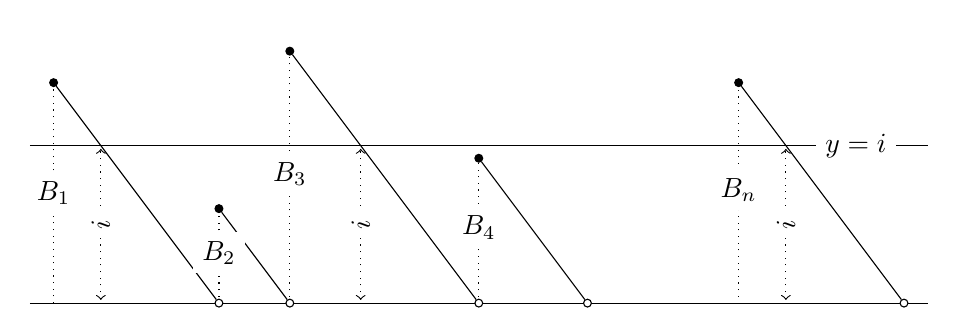
\begin{tikzpicture}[yscale=0.8,xscale=0.6,
 open/.style={shape=circle, fill=white, inner sep=1pt, draw, node contents=},
 closed/.style={shape=circle, fill=black, inner sep=1pt, draw, node contents=}]

 % y = zero line
 \draw (-0.5, 0) -- (18.5, 0); 
 % level crossing
 \draw (-0.5, 2.5) -- (18.5, 2.5) 
 %node[pos=0.65, fill=white, above] {$\sum_{k=1}^n \1{B_k \geq i}$}
 node[pos=0.92, fill=white] {$y=i$};


 \draw node (c1) at (0,3.5) [closed, label={}]
 node (c2) at (3.5,0)[open, label={}]
 (c1) to (c2);
 \draw[dotted] (0,0) -- (0,3.5) node[midway, fill=white] {$B_1$};
 \draw[dotted, <->] (1, 0.05) -- (1, 2.45) node[fill=white, midway, rotate=90] {$i$};


 \draw node (c1) at (3.5,1.5) [closed, label={}]
 node (c2) at (5,0)[open, label={}]
 (c1) to (c2);
 \draw[dotted] (3.5,0.1) -- (3.5,1.5) node[midway, fill=white] {$B_2$};

 \draw node (c1) at (5,4) [closed, label={}]
 node (c2) at (9,0)[open, label={}]
 (c1) to (c2);
 \draw[dotted] (5,0.1) -- (5,4) node[midway, fill=white] {$B_3$};
 \draw[dotted, <->] (6.5, 0.05) -- (6.5, 2.45) node[fill=white, midway, rotate=90] {$i$};

 \draw node (c1) at (9,2.3) [closed, label={}]
 node (c2) at (11.3,0)[open, label={}]
 (c1) to (c2);
 \draw[dotted] (9,0.1) -- (9,2.3) node[midway, fill=white] {$B_4$};

 % end
 \draw node (c1) at (14.5,3.5) [closed, label={}]
 node (c2) at (18,0)[open, label={}]
 (c1) to (c2);
 \draw[dotted] (14.5,0.1) -- (14.5,3.5) node[midway, fill=white ] {$B_n$};
 \draw[dotted, <->] (15.5, 0.05) -- (15.5, 2.45) node[fill=white, midway, rotate=90] {$i$};
 

 % bottom line
 %\draw[<->] (0, -0.6) -- (18, -.6) node[fill=white, midway] {$\sum_{k=1}^n B_k$};
\end{tikzpicture}

\caption{A batch crosses the line $y=i$ iff it contains at least $i$ items.
 Thus, during the service of a batch with $i$ or more items, there is precisely one service of an $i$-th item.}
 \label{fig:remainingservicetime}
\end{figure}


\begin{exercise}\clabel{ex:l-170}
 Now use the renewal reward theorem to show that the (time-average) fraction of time there are~$i$ items at the server is equal to
 \begin{equation*}
 \P{L_S = i} = \lambda \E{S} G(i-1) = \rho \frac{G(i-1)}{\E B}.
 \end{equation*}
Conclude that
\begin{equation*}
 \E{L_S} = \sum_{i=0}^\infty i \P{L_S=i} = \frac{\rho}{\E B} \sum_{i=1}^\infty i G(i-1).
\end{equation*}
\begin{solution}
 By construction, $Y_i(t)/t \to \P{L_S=i}$.
 Let $X_k = Y_i(D_k) - Y_i(D_{k-1})$.
 Then, since the $\{S_{k, i}\}$ are i.i.d. with $\E{S_{k,i}} = \E S$, 
 and the $\{B_k\}$ are i.i.d., we obtain from the previous exercise that $X = \lim_{n\to\infty} n^{-1}\sum_{k=1}^n (S_{k,i} \1{B_{k} \geq i}) = \E{S \1{B\geq i}}$.
 Now $B$ and $S$ are independent by assumption, hence $X = \E{S} \E{\1{B\geq i}} = \E S \P{B\geq i}$.
 The result follows by using rate stability ($\delta = \lambda$) in the renewal reward theorem.
\end{solution}
\end{exercise}



\begin{extra}\clabel{ex:ER}
 Show that
 \begin{equation*}
 \sum_{i=1}^\infty i G(i-1)= \frac{\E{B^2} + \E B}{2},
\end{equation*}
so that
\begin{equation*}
 \E{L_S} = \rho \frac{\E{B^2}}{2 \E B} + \frac{\rho}{2}.
\end{equation*}

\begin{hint}
 Use~\cref{ex:6} and~\cref{ex:66}.
\end{hint}
\begin{solution}
\begin{equation*}
 \begin{split}
 \sum_{i=1}^\infty i G(i-1) 
&=\sum_{i=0}^\infty (i+1) G(i) 
=\sum_{i=0}^\infty i G(i) +
\sum_{i=0}^\infty G(i)\\
&= (\E{B^2} - \E B + 2\E B)/2.
 \end{split}
\end{equation*}
\end{solution}
\end{extra}
  
\end{comment}


\opt{solutionfiles}{
\Closesolutionfile{hint}
\Closesolutionfile{ans}
\subsection*{Hints}
\input{hint}
\subsection*{Solutions}
\input{ans}
}

%\clearpage

%%% Local Variables:
%%% mode: latex
%%% TeX-master: "../companion"
%%% End:


%\section{$M/G/1$ Queue: Expected Waiting Time}
%{$\mathbf{M/G/1}$ Queue: Expected Waiting Time}
\label{sec:mg1}


\subsection*{Theory and Exercises}

\Opensolutionfile{hint}
\Opensolutionfile{ans}


Let's focus on one queue in a supermarket, served by one cashier, and assume that customers do not jockey, i.e., change queue.
What can we say about the average waiting time in queue if service times are not exponential, like in the $M/M/1$ queue, but have a more general distribution?
One of the celebrated results of queueing theory is the Pollaczek-Khinchine formula by which we can compute the average waiting time formula for the $M/G/1$ queue.
In this section we derive this result by means of sample path arguments.

Recall that Eq.~\eqref{eq:35} states that
\begin{equation*}
  \E{W_Q} = \frac{\E{S_r}}{1-\rho}.
\end{equation*}
It remains to compute the average remaining service time $\E{S_r}$ for generally distributed service times. For this, we use the renewal reward theorem, again.


Consider the $k$th job of some sample path the $M/G/1$ queueing process.
This job requires $S_k$ units of service, let its service time start at time $\tilde A_k$ so that it departs the server at time $D_k=\tilde A_k + S_k$. 
\begin{exercise}[\faFlask]
Use  Figure~\ref{fig:mg1remainingservicetime} to explain that job $k$the remaining service time at time $s$ is given by
\begin{equation*}
R_k(s) = (D_k-s)\1{\tilde A_k \leq s < D_k}.
\end{equation*}
\begin{solution}
Observe that when $s\in [\tilde A_k, D_k)$, the remaining service
time until job $k$ departs is $D_k-s $, while if
$s\not \in [\tilde A_k, D_k)$, job $k$ is not in service so it cannot have
any remaining service.
\end{solution}
\end{exercise}

\begin{exercise}[\faFlask]
  Explain that
  \begin{equation*}
    Y(t) = \int_0^t (D_{D(s)+1}-s)\1{L(s) > 0} \d s
  \end{equation*}
is the total remaining service time as seen by the server up to $t$. 
\begin{solution}
  At time $s$, the number of departures is $D(s)$. Thus, $D(s)+1$ is the first job to depart after time $s$. The departure time of this job is $D_{D(t)+1}$, hence the remaining service time at time $s$ is $D_{D(s)+1}-s$, provided this job is in service. 
\end{solution}
\end{exercise}

\begin{figure}[htb]
  \centering
\begin{tikzpicture}[scale=1,
  open/.style={shape=circle, fill=white, inner sep=1pt, draw, node contents=},
  closed/.style={shape=circle, fill=black, inner sep=1pt, draw, node contents=}]
    \draw (-1,0) -- (4,0); 
    %x\draw (1,0) -- (3,0) node[midway, fill=white] {$s$};
    \draw node (c1) at (0,3) [closed, label={}]
          node (c2) at (3,0)[open, label={}]
     (c1) to (c2);
    \draw[dotted] (0,0) -- (0,3) node[midway, rotate=90, fill=white] {$S_k$};
    \node[below] at (0,0) {$\tilde A_k$};
    \node[below] at (3,0) {$D_k$};

    \draw[<->, dotted] (0.75,0) -- (0.75,2.25) node[midway,fill=white,rotate=90] {$D_k-s$};
    \node[below] at (0.75,0) {$s$};
  \end{tikzpicture}

  \caption{Remaining service time.}
  \label{fig:mg1remainingservicetime}
\end{figure}

\begin{exercise}[\faCalculator]
Use the renewal reward theorem to prove that 
\begin{equation}\label{eq:34}
\E{S_r} = \frac{\lambda}2 \E{S^2}.
\end{equation}
\begin{hint}
  Choose $T_k=D_k$ as epochs in the renewal reward theorem.
\end{hint}
\begin{solution}
  It is clear that the time-average $Y(t)/t \to \E{S_r}$. Moreover, $X_k = Y(D_k) - Y(D_{k-1})$ is the area under the triangle in Figure~\ref{fig:mg1remainingservicetime}. Thus,
  $X=\lim_{n\to\infty} \lim_{k=1}^n S_k^2/ 2 = \E{S^2}/2$. Finally,  $\delta = \lambda$ by rate-stability.
\end{solution}
\end{exercise}

\begin{exercise}[\faCalculator]
Use $C_s^2 = \V S / (\E S)^2$ to show that $\lambda \E{S^2} = (1+C_s^2)\rho\E S$
\begin{solution}
Use that 
\begin{equation*}
  \frac{\E{S^2}}{(\E S)^2} = 
  \frac{(\E{S^2}-(\E S)^2) + (\E S)^2}{(\E S)^2} =
  \frac{\V S + (\E S)^2}{(\E S)^2} =
  C_s^2 + 1.
\end{equation*}
Then
\begin{equation*}
  \lambda\E{S^2} = \frac{\E{S^2}}{(\E S)^2} \lambda(\E S)^2=
 \frac{\E{S^2}}{(\E S)^2} \rho \E S = (1+C_s^2) \rho \E{S}.
\end{equation*}
\end{solution}
\end{exercise}


With the above exercises  we have obtained the fundamentally important \recall{Pollaczek-Khinchine formula} for the average waiting time in queue:
\begin{equation} \label{eq:710}
  \E{W_Q} = \frac{\E{S_r}}{1-\rho} =\frac 1 2 \frac{\lambda \E{S^2}}{1-\rho} =\frac{1 + C_s^2}2 \frac{\rho}{1-\rho}  \E S.
\end{equation}
The problems below will illustrate how useful this result is.


\begin{exercise}[\faFlask]
\label{ex:9}
Show from Eq.~\eqref{eq:34} that 
\begin{equation}\label{eq:55}
\E{S_r\given S_r>0} = \frac{\E{S^2}}{2 \E S}.
\end{equation}
\begin{solution}
 From Eq.~\eqref{eq:37} and the sentences above this equation,
    we have that
    \begin{equation*}
    \E{S_r} = \rho \E{S_r\given S_r>0}=\lambda \E S \E{S_r\given S_r>0}.
    \end{equation*}
Hence,
    \begin{equation*}
    \lambda \E{S_r\given S_r>0} = \frac{\E{S_r}}{\E S} = \lambda \frac{\E{S^2}}{2 \E S}.
    \end{equation*}
\end{solution}
\end{exercise}


\begin{exercise}[\faFlask]
Show that  $\E {S_r\given S_r>0} = \alpha/2$  when $\V{S} = 0$ (hence $\E S = \alpha$).
  \begin{hint}
    $\V S = 0$ implies that $S$ is deterministic.
  \end{hint}
\begin{solution}
 When $S$ is deterministic $\E S= \alpha$ and $\E{S^2} = \alpha^2$.  Now use~\eqref{eq:55}.
\end{solution}
\end{exercise}

\begin{exercise}[\faCalculator]
Show that $\E{S_r\given S_r>0} = \alpha/3$ when  $S \sim U[0, \alpha]$.
\begin{solution}
 When $S$ is uniform on $[0, \alpha]$,
 \begin{align*}
    \E S &= \alpha^{-1}\int_0^\alpha x \, \d x =\frac{\alpha^2}{2 \alpha} =  \frac{\alpha}2, 
&
\E{S^2} &= \alpha^{-1}\int_0^\alpha x^2 \, \d x = \frac{\alpha^2}3.   
 \end{align*}
 Thus, with~\eqref{eq:55}, $\E{S_r\given S_r>0} = (\alpha^2/3)/(2 \alpha/2) = \alpha/3$. 
\end{solution}
\end{exercise}

\begin{exercise}{\faFlask}
 Show that $\E{S_r\given S_r>0} = \mu^{-1}$ when $S\sim \Exp(\mu)$.
\begin{solution}
    \begin{align*}
\E S &= \mu \int_0^\infty x e^{-\mu x}\,\d x = 1/\mu, \\
\E{S^2} 
&= \mu \int_0^\infty x^2 e^{- \mu x} \,\d x = - \left. x^2 e^{-\mu x} \right|_0^\infty + 2 \int_0^\infty x e^{-\mu x} \, \d x \\
&= -\left. 2\frac x \mu e^{-\mu x} \right|_0^\infty + \frac 2 \mu\int_0^\infty e^{-\mu x} \, \d x =\frac2{\mu^2}.
    \end{align*}
\end{solution}
\end{exercise}


\begin{exercise}[\faFlask]
  Show that when services are exponential, the expected waiting time
  $\E{W_Q(M/G/1)}$ reduces to $\E{W_Q(M/M/1)}$.
    \begin{solution}
      Since the SCV for the exponential distribution is $1$, hence
      $C_s^2=1$, we get 
    \begin{equation*}
\E{W_Q} = \frac{1+1}2\frac{\rho}{1-\rho} \E S = \frac{\rho}{1-\rho} \E S,
    \end{equation*}
which we also found in a previous section.
    \end{solution}
\end{exercise}


\begin{exercise}[\faCalculator]
  Compute $\E{W_Q}$ and $\E L$ for the $M/D/1$ queue. Assume that the
  service time is always~$T$. Compare $\E{L(M/D/1)}$ to $\E{L(M/M/1)}$
  where the mean service time is the same in both cases.
\begin{solution}
  For the $M/D/1$ the service time is deterministic. Thus, the service time $S=T$ always; recall that $S$ is   deterministic under the assumptions in the exercise. Therefore, we
  must have that $\P{S\leq T} = 1$. As an immediate consequence,
  $\P{S>T} = 1-\P{S\leq T} = 0$. Also, $\P{S \leq x} = 0$ for all
  $x<T$. Thus, all probability mass is concentrated on the point $T$,
  thus, it is also impossible that the service time is smaller than
  $T$.  (If you are into mathematics, then you should be aware of the fact
  that `impossible' and `almost surely' are not the same. Thus, my
  using of the word `impossible' is not completely correct.)

  To compute the SCV, I first compute $\E S$, then $\E{S^2}$ and then
  $\V S = \E{S^2} - \left(\E S\right)^2$, and use the definition of
  coefficient of variation. I use these steps time and again.

  First, $\E S = T$ since $\P{S=T} =1$. We can also obtain this in a
  more formal way. The distribution $F(x)$ of $S$ has a, so-called, atom at
  $x=T$, such $F(T) - F(T-) =1$.  Using this,
  \begin{equation*}
    \E S = \int_0^\infty x \d F(x) = T\cdot (F(T)-F(T-)) = T.
  \end{equation*}
Similarly
\begin{equation*}
\E{S^2} = \int_0^\infty x^2 \d F(x) = T^2\cdot (F(T)-F(T-)) = T^2.
\end{equation*}
Hence $\V S = \E{S^2} - (\E S)^2 = 0$, hence $C_s^2 = 0$.

From the Pollaczek-Khinchine formula, the first term is $1+C_s^2=1$ for the $M/D/1$ queue, and $1+C_s^2=2$ for the $M/M/1$ queue. Hence, 
  \begin{equation*}
\E{W_Q(M/D/1)} = \frac{\E{W_Q(M/M/1)}}2.
  \end{equation*}
Thus, 
\begin{equation*}
 \E{L_Q(M/D/1)} = \frac{\E{L_Q(M/M/1)}}2.    
\end{equation*}
In both cases the expected service times are equal to $T$ so that the loads are the same. Thus, 
\begin{equation*}
  \begin{split}
 \E{L(M/D/1)} &= \E{L_Q(M/D/1)} +\rho = \frac{\E{L_Q(M/M/1)}}2 + \rho \\
&= \frac{\rho^2}{2(1-\rho)} + \rho=\frac{\rho(2-\rho)} {2(1-\rho)}.
  \end{split}
\end{equation*}
\end{solution}
\end{exercise}

\begin{exercise}[\faCalculator]
  Compute $\E L$ for the $M/G/1$ queue with $S\sim U[0,\alpha]$.
  \begin{hint}
Integrate $\alpha^{-1} \int x \d x$, and likewise for the second moment.
  \end{hint}
\begin{solution}
  \begin{align*}
\E S &= \alpha/2,\\
\E{S^2} &= \int_0^\alpha x^2 \d x/\alpha = \alpha^2/3\\
\V S &= \alpha^2/3 - \alpha^2/4= \alpha^2/12\\
C_s^2 &= (\alpha^2/12)/(\alpha^2/4) = 1/3,\\
\rho &= \lambda \alpha/2,\\
\E{W_Q} &= \frac{1+C_s^2}2 \frac{\lambda \alpha/2}{1-\lambda \alpha/2}\frac \alpha2, \\
\E W &= \E{W_Q} + \frac \alpha2\\
\E L &= \lambda \E W.
  \end{align*}
\end{solution}
\end{exercise}

\begin{exercise}[\faPhoto]
  A queueing system receives Poisson arrivals at the rate of 5 per
  hour. The single server has a uniform service time distribution,
  with a range of 4 minutes to 6 minutes. Determine $\E{L_Q}$, $\E L$,
  $\E{W_Q}$, $\E W$.
  \begin{solution}
First the load.
\begin{pyconsole}
labda = 5./60 # arrivals per minute
a = 4.
b = 6.
ES = (a+b)/2.  # service time in minutes
rho = labda*ES
rho
\end{pyconsole}

Next, the variance and SCV. With this the waiting times follow right away.
\begin{pyconsole}
Var = (b-a)*(b-a)/12.
SCV = Var/(ES**2)


Wq = (1+SCV)/2.*rho/(1.-rho)*ES
Wq # in minutes
Wq/60. # in hour


W = Wq + ES
W
Lq = labda*Wq
Lq
L = labda*W
L
\end{pyconsole}
  \end{solution}
\end{exercise}



\begin{exercise}[\faPhoto]
  Consider a workstation with just one machine. Jobs arrive, roughly,
  in accordance with a Poisson process, with rate $\lambda=3$ per day. The
  average service time $\E S = 2$ hours, $C^2_s = 1/2$, and the shop
  is open for 8 hours. What is $\E{W_Q}$?

 Suppose the expected waiting time has to be reduced to 1h. How
  to achieve this? 
\begin{solution}
  $\E{W_Q} = 4.5$ h. $\rho = \lambda \E S = (3/8)\cdot 2 = 3/4$.

 One way to increase the capacity/reduce the average service
    time is to choose $\E S =1$ hour and reduce $C^2_s$ to $1/4$.  Of
    course, there are many more ways. Reducing $C^2_S$ to zero is
    (nearly) impossible or very costly. Hence, $\rho$ must go down,
    i.e., capacity up or service time down. Another possibility is to
    plan the arrival of jobs, i.e., reduce the variability in the
    arrival process. However, typically this is not possible. For
    instance, would you accept this as a customer?
\end{solution}
\end{exercise}


\begin{exercise}[\faPhoto]
  (Hall 5.16) The manager of a small firm would like to determine
  which of two people to hire. One employee is fast, on average, but
  is somewhat inconsistent. The other is a bit slower, but very
  consistent. The first has a mean service time of $2$ minutes, with a
  standard deviation of 1 minute. The second has a mean service time
  of $2.1$ minutes, with a standard deviation of $0.1$ minutes. If the arrival rate is Poisson with rate 20 per hour, which employee would minimize $\E{L_Q}$? Which would minimize $\E L$? 
  \begin{solution}
    The arrival process is assumed to be Poisson. There is also
    just one server. Hence, we can use the PK formula to compute the average queue length.

\begin{pyconsole}
labda = 20./60 # per minute
ES = 2. # minutes
sigma = 1.
SCV = sigma*sigma/(ES*ES)
rho = labda*ES
rho

Wq = (1+SCV)/2 * rho/(1-rho) * ES
Wq
Lq = labda * Wq # Little's law
Lq
W = Wq + ES
W
L = labda * W
L
\end{pyconsole}


\begin{pyconsole}
ES = 2.1
SD = 0.1
SCV = SD**2/ES**2
rho = labda*ES
rho

Lq = rho**2/(1.-rho)*(1.+SCV)/2.
Lq
L = rho + Lq
L
\end{pyconsole}

  \end{solution}
\end{exercise}


\begin{exercise}[\faFlask]
  Show that for the $M/G/1$ queue, the expected idle time is
  $\E I = 1/\lambda$.  
  \begin{hint}
What is the average time between two
    arrivals? Observe that the inter-arrivals are memoryless, hence the
    average time until the next arrival after the server becomes idle
    is also $1/\lambda$.
  \end{hint}
  \begin{solution}
    Since the inter-arrival times are memoryless, the expected time to the first arrival after the system becomes empty is also $\E X=1/\lambda$.
  \end{solution}
\end{exercise}

\begin{exercise}[\faFlask]
  What is the utilization of the $M/G/1/1$ queue?  
  \begin{solution}
    The system can contain at most 1 job.
    Necessarily, if the system contains a job, this job must be in service.
    All jobs that arrive while the server is busy are rejected.
    Just after a departure, the average time until the next arrival is $1/\lambda$, and then a new service starts with an average duration of $\E S$.
    After this departure, a new cycle starts.
    Thus, the utilization is $\E S/(1/\lambda + \E S) = \lambda \E S/ (1 + \lambda \E S)$.
    Since not all jobs are accepted, the utilization $\rho$ cannot be equal to $\lambda \E S$.
  \end{solution}
\end{exercise}

\begin{exercise}[\faFlask]
  For the $M/G/1/1$ queue what is the fraction of jobs rejected
  (hence, what is the fraction of accepted jobs)?  
  \begin{hint}
The rate of
    accepted jobs is $\lambda \pi(0)$. What is the load of these jobs?
    Equate this to $1-\pi(0)$ as this must also be the load. Then solve for $\pi(0)$.
  \end{hint}
  \begin{solution}
    Let $p(0)$ be the fraction of time the server is idle. By PASTA,
    $\pi(0)=p(0)$. Thus, the rate of accepted jobs is
    $\lambda\pi(0)$. Therefore, the departure rate
    $\delta=\lambda\pi(0)$. The loss rate is
    $\lambda-\delta = \lambda (1-\pi(0))$.

    Since $\lambda\pi(0)$ is the rate at which jobs enter the system,
    the load must be $\lambda\pi(0)\E S$. Since the load is also
    $1-\pi(0)$, it follows from equating that
    \begin{equation*}
      \lambda\pi(0) \E S = 1 - \pi(0) \iff \pi(0)=\frac1{1+\lambda\E S} 
\iff 1-\pi(0) = \frac{\lambda \E S}{1+\lambda \E S},
    \end{equation*}
which is the same as in the previous problem.

Note that  $\delta < \lambda$, as it should be the case. 
  \end{solution}
\end{exercise}


\begin{exercise}[\faFlask]
  Why is the fraction of lost jobs at the $M/G/1/1$ queue not
  necessarily the same as for a $G/G/1/1$ queue with the same load?  
  \begin{hint}
Provide an  example.
  \end{hint}
  \begin{solution}
 Typically, in the $G/G/1$ queue, the arrivals do not see  time-averages. Consequently, the fraction of arrivals that are blocked is not necessarily equal to the utilization~$\rho$.

  Again, take jobs with a duration 59 minutes and inter-arrival times of
  1 hour. The load is $59/60$, but no job is lost, also not in the
  $G/G/1/1$ case. Thus, $\delta=\lambda$ in this case.
  \end{solution}
\end{exercise}





\Closesolutionfile{hint}
\Closesolutionfile{ans}

\opt{solutionfiles}{
\subsection*{Hints}
\input{hint}
\subsection*{Solutions}
\input{ans}
}

%\clearpage




%%% Local Variables:
%%% mode: latex
%%% TeX-master: "../queueing_book"
%%% End:

%\section{$M^X/M/1$ Queue Length Distribution}
%{$\mathbf{M^X/M/1}$ Queue Length Distribution}
\label{sec:batch-arrivals}




\opt{solutionfiles}{
\subsection*{Theory and Exercises}
\Opensolutionfile{hint}
\Opensolutionfile{ans}
}

In~\cref{sec:mxm1-queue:-expected,sec:mg1} we established the Pollaczek-Khinchine formula for the waiting times of the $M^X/M/1$ queue and $M/G/1$ queue, respectively.
To compute more difficult performance measures, for instance the loss probability $\P{L>n}$, we need expressions for the stationary distribution $\pi(n)=\P{L=n}$ of the number of jobs in the system.
Here we present a numerical, recursive, scheme to compute these probabilities.

To find $\pi(n)$, $n=0, 1, \ldots$, we turn again to level-crossing arguments.
However, the reasoning that lead to the level-crossing equation~\cref{eq:15} need to be generalized.
To see this, we consider an example.
If $L(t)=3$, the system contains $3$ items.
(This is not necessarily the same as 3 batches.)
Since the server serves single items, down-crossings of level $n=3$ occur in single units.
However, due to the batch arrivals, when a job arrives it typically brings multiple items to the queue.
For instance, suppose that $L(A_k-) = 3$, i.e., job $k$ sees 3 items in the system at its arrival epoch.
If it's size $B_k = 20$, then right after the $k$th arrival the system contains 23 items, that is, $L(A_k)=3+20=23$.
Thus, at the arrival of job $k$, all levels between states $3$ and $23$ are crossed.

The left panel in~\cref{fig:levelcrossing} shows all up- and down-crossings of some level $n$.
The down-crossing rate is easy: just as in~\cref{fig:A_n_t} there is just one arrow from right to left.
However, level~$n$ can be up-crossed from below from many states, in fact from any level $m, 0\leq m <n$.
More formally, to count the number of up-crossings define
\begin{equation*}
  A(m,n,t) = \sum_{k=1}^{A(t)}\1{L(A_k-) = m}\1{B_k > n-m}
\end{equation*}
as the number of jobs up to time $t$ that see $m$ in the system upon arrival and have batch size larger than $n-m$.
% With this, the total number of times level $n$ is up-crossed up to time~$t$ becomes
%  \begin{equation*}
% A(n, t) =  \sum_{m=0}^n A(m,n,t).
% \end{equation*}


% Observe that $\1{L(A_k-)\leq n}=1$ only when the $k$th job sees~$n$ or less items in the system, and $\1{L(A_k) > n}=1$ only after the $k$th arrival the system contains more than $n$ items.
% Thus, $\1{L(A_k-) \leq n}\1{ L(A_k)>n}=1$ iff the $k$th arrival generates an up-crossing of level~$n$.

% %  Hence
% % \begin{equation*}
% %   \sum_{k=1}^{A(t)} \1{L(A_k-) \leq n}\,\1{L(A_k)>n}
% % \end{equation*}
% % counts all up-crossings  of level $n$ up to time $t$.


% From~\cref{fig:levelcrossing} we see that an up-crossing can be decomposed into:
% \begin{equation*}
%   \begin{split}
% &\1{L(A_k-) \leq n}\1{L(A_k)>n}  \\
% &=  \1{L(A_k-) =n}\, \1{B_k >0} + \1{L(A_k-) =n-1}\1{ B_k >1} +\cdots + \1{L(A_k-) =0}\1{B_k > n} \\
% &= \sum_{m=0}^n \1{L(A_k-) =m}\1{B_k > n-m}.
%   \end{split}
% \end{equation*}
% In other words, sample paths that up-cross level $n$ require that any job that
% sees $m$ ($m\leq n$) in the system upon arrival must bring a batch larger
% than $n-m$ items.



% As a consequence, it is not
% necessarily the case that $|A(n,t) - D(n,t)| \leq 1$ for all $t$, as
% was the case for queueing systems in which jobs arrive as single
% units. We need to generalize this inequality.

\begin{figure}[ht]
  \centering
\begin{tikzpicture}[scale=1,
    %Define standard arrow tip
    >=stealth',
    %Define style for boxes
    circ/.style={
      circle, 
      draw=black,
      thick,
      minimum size=1.cm,
      inner sep=0pt,
      text centered
    },
    % Define arrow style
    pil/.style={
           ->,
           thick,
           shorten <=2pt,
           shorten >=2pt}
]

\draw[dashed, thick] node at (5,-1.5) [below]  {level $n$} 
(5,-1.5) -- (5,3);

\node[circ] (n-2) {$n-2$};

%\node[circ, right=of n-2] (n-1) {$n-1$} edge[loop below, thick] node[midway, fill=white] {$\lambda f(0)$} (n-1);
\node[circ, right=of n-2] (n-1) {$n-1$};

\node[circ, right=of n-1] (n) {$ n $}
   edge[pil,<-, bend left=45] node[below] {$\lambda f(1)$} (n-1.south east);
\node[circ, right=of n] (n+1) {$n+1$}
   edge[pil,bend left=45] node[midway, fill=white] {$\mu$} (n.south east);
\node[above=of n+1] (inf) {}
   edge[pil, <-, bend right=45] node[midway, fill=white] {$\lambda G(0)$} (n.north east)
   edge[pil, <-, bend right=45] node[midway, fill=white] {$\lambda G(1)$} (n-1.north east)
   edge[pil, <-, bend right=45] node[midway, fill=white] {$\lambda G(2)$} (n-2.north east)
;
\end{tikzpicture}
%  \begin{tabular}
%    \includegraphics[scale=0.9]{mxm1_2}
%&
%    \includegraphics[scale=0.9]{mxm1_1}
%  \end{tabular}
\caption{Level crossing of level $n$.
  Observe that when the system is in state $n-2$, the arrival of any batch larger than $2$ ensures that level $n$ is crossed from below.
  The rate at which such events happen is $\lambda \pi(n-2) G(2)$.
  Similarly, in state $n-1$ the arrival of any batch larger than one item ensures that level $n$ is crossed, and this occurs with rate $\lambda \pi(n-1) G(1)$, and so on.
}
  \label{fig:levelcrossing}
\end{figure}

\begin{extra}
   Show that $A(n, n,t) = A(n,t)$, where $A(n,t)$ is defined by~\cref{eq:19}.
\begin{solution}
 $A(n,n,t)$ counts all jobs up to time $t$ that see $n$ items
    and bring at least $n-n+1=1$ unit of work. As each job brings at
    least 1 item, $A(n,n,t)$ counts all jobs that see $n$ items at
    arrival.
\end{solution}
\end{extra}

\begin{exercise}\clabel{ex:70}
Assuming that the limits exist, show that
\begin{equation*}
\lim_{t\to\infty}   \frac{A(m,n,t)}t = \lambda \pi(m) G(n-m).
\end{equation*}
\begin{solution}
For this purpose, observe that we can write
\begin{equation}\label{eq:16}
  \frac{A(m,n,t)}t =   \frac{A(t)}t \frac{A(m,t)}{A(t)}\frac{A(m,n,t)}{A(m,t)}.
\end{equation}
By the assumptions of~\cref{sec:poisson-arrivals-see}, $A(t)/t\to\lambda$ and $A(m,t)/A(t)\to\pi(m)$.
Next, apply the results of~\cref{ex:68} to~\cref{ex:69}.
\end{solution}
\end{exercise}

\begin{extra}\clabel{ex:68}
Provided the limit exists, show that
\begin{equation}\label{eq:1332}
\lim_{t\to\infty} \frac{A(m,n,t)}{A(m,t)} =\P{B>n-m\given L(A-)=m},
\end{equation}
where the random variable $L(A-)$ denotes the number in the system seen by an arbitrary arrival.
\begin{solution}
\begin{equation*}
\lim_{t\to\infty} \frac{A(m,n,t)}{A(m,t)} = 
\lim_{t\to\infty} \frac{\sum_{k=1}^{A(t)}\1{L(A_k-) = m, B_k > n-m}}
{\sum_{k=1}^{A(t)}\1{L(A_k-) = m}}=\P{B>n-m\given L(A-)=m},
\end{equation*}
\end{solution}
\end{extra}


\begin{extra}\clabel{ex:69}
Show that $\P{B>n-m\given L(A-)=m}=\P{B>n-m}$.
\begin{hint}
    Realize that $B$ and $L(A-)$ are assumed to be independent.
\end{hint}
\begin{solution}
\begin{equation*}
  \begin{split}
\P{B>n-m\given L(A-)=m} &=
\frac{\P{B>n-m,L(A-)=m}}{\P{L(A-)=m}}\\
&=\frac{\P{B>n-m}\P{L(A-)=m}}{\P{L(A-)=m}} \\
&= \P{B>n-m} =G(n-m).
  \end{split}
\end{equation*}
\end{solution}
\end{extra}

Equating the number of up- and down-crossing gives $\sum_{m=0}^n A(m,n,t) \approx  D(n,t)$. 
Then, dividing by~$t$,  taking the limit $t\to\infty$, and using~\cref{ex:70} results in the level-crossing equation for the $M^X/M/1$ queue:
\begin{equation}\label{eq:42}
\lambda  \sum_{m=0}^n \pi(m) G(n-m) = \mu \pi(n+1).
\end{equation}

\begin{exercise}\clabel{ex:l-153}
Provide an interpretation of~\cref{eq:42} in terms of a thinned Poisson arrival process.
\begin{solution}
  \Cref{eq:16} has the interpretation that the rate at which level $n$ is crossed from below from state $m$ is equal to the rate at which jobs arrive times the fraction of jobs that see $m$ jobs in the system times the fraction of jobs with batch size larger than $n-m$.
  Observe that the stream of jobs with batch size larger than $n-m$ is a Poisson process thinned at rate $G(n-m)$.
\end{solution}
\end{exercise}


\begin{extra}
  Show that~\cref{eq:42} reduces to $\mu \pi(n+1)=\lambda \pi(n)$ for the $M/M/1$ case.
\begin{solution}
    The right-hand side of~\cref{eq:42} is identical, so we only have to concentrate on the left-hand side.
    In the $M/M/1$ queue, all batches have size $1$.
    Thus, $\P{B=1} = f(1)=1$ and $f(k)=0$ for $k\neq 1$.
    Thus, $G(0)=1$ and $G(1)=G(2)=\cdots = 0$.
    Thus, $\sum_{m=0}^n G(n-m) \pi(m) = G(0)\pi(n)=\pi(n)$.
\end{solution}
\end{extra}



It is left to find the normalization constant.
As this recursion does not lead to a closed form expression for $\pi(n)$, such as~\cref{eq:23}, we need to use a criterion to stop this iterative procedure.
Finding general conditions when to stop is not directly easy, but a pragmatic approach is simple.
When the demand is finite, the numbers $\{\pi(k)\}$ should decrease geometrically fast when $k\geq N$ for some (large) $N$\footnote{An interesting question, why should it decrease monotonically after some, large, $N$?}.
Stop when $\pi(N)\ll \pi(0)$, and take $G=\sum_{i=0}^N \pi(i)$ as the normalization constant.
While this is a practical approach, getting formal bounds on a proper size of $N$ requires more work than we can do here.

Once again with $\pi(n)$ we can compute all performance measures we need, and study the influence on the batch size distribution and $\lambda$ and $\mu$ on the system's performance.

\begin{exercise}\clabel{ex:l-154}
  Why is~\cref{eq:39}, i.e., $\pi(n)=\delta(n)$, not true for the $M^X/M/1$ batch queue?
  Provide an example.
\begin{solution}
 Because arrivals do not occur in single units, but in batches.
\end{solution}
\end{exercise}

\begin{exercise}\clabel{ex:73}
 Substitute recursion~\cref{eq:42} for $\pi(n)$ into the expression $\E{L} = \sum_{n=0}^\infty n \pi(n)$ and derive~\cref{eq:43}.
\begin{solution}
    We chop this up into two steps, see~\cref{ex:71} and~\cref{ex:72}.
\end{solution}
\end{exercise}

\begin{extra}\clabel{ex:71}
  Step 1 of~\cref{ex:73}.
  Show that
\begin{equation}\label{eq:67}
  \mu \E L =\mu \sum_{n=0}^\infty n \pi(n) = \lambda \frac{\E{B^2}}2  + \lambda \E B \E L +\lambda \frac{\E B}2.
\end{equation}
\begin{hint}
  Substitute the recursion, and carry on with the algebra.
  Use also the results of the exercises of~\cref{sec:mxm1-queue:-expected}.
\end{hint}
\begin{solution}
  We use that $\mu \pi(n) =\lambda \sum_{i=0}^{n-1} \pi(i) G(n-1-i)$ and the results of the exercises of~\cref{sec:mxm1-queue:-expected} to see that
\begin{align*}
  \mu \E L
  &=\sum_{n=0}^\infty n\, \mu \pi(n), \quad \text{now substitute for $\mu \pi(n)$ the recursion~\cref{eq:42}}, \\
& =\lambda \sum_{n=0}^\infty n \sum_{i=0}^{n-1} \pi(i) G(n-1-i) 
  =\lambda \sum_{n=0}^\infty n \sum_{i=0}^\infty \1{i<n} \pi(i) G(n-1-i) \\
& =\lambda \sum_{i=0}^\infty \pi(i) \sum_{n=0}^\infty \1{i<n} n G(n-1-i) 
  =\lambda \sum_{i=0}^\infty \pi(i) \sum_{n=i+1}^\infty n G(n-1-i) \\
& =\lambda \sum_{i=0}^\infty \pi(i) \sum_{n=0}^\infty (n+i+1) G(n) 
  =\lambda \sum_{i=0}^\infty \pi(i) \left[\sum_{n=0}^\infty n G(n) +(i+1) \sum_{n=0}^\infty G(n)\right]  \\
  &=\lambda \sum_{i=0}^\infty \pi(i)\sum_{n=0}^\infty n G(n) +\lambda  \E B \sum_{i=0}^\infty \pi(i) (i+1)  \\ 
  &=\lambda \sum_{i=0}^\infty \pi(i) \frac{\E{B^2} -\E B}2  + \lambda \E B (\E L +1)  \\ 
  &= \lambda \frac{\E{B^2} -\E B}2  + \lambda \E B \E L +\lambda \E B \\
  &= \lambda \frac{\E{B^2} }2  + \lambda \E B \E L +\lambda \frac{\E B}2.
\end{align*}
\end{solution}
\end{extra}

\begin{extra}\clabel{ex:72}
  Step 2 of~\cref{ex:73}.
  Use~\cref{eq:67} and the definition $\rho=\lambda \E B/\mu$ to show that
\begin{equation*}
(1- \rho) \E L = \frac{\lambda}\mu \frac{\E{B^2}}2 + \frac\rho2.
\end{equation*}
\begin{solution}
  Dividing both sides of~\cref{eq:67} by $\mu$ and using that $\lambda \E B/\mu = \rho$,
\begin{equation*}
  \E L = \frac{\lambda}{\mu}  \frac{\E{B^2}}2 + \rho \E L + \frac\rho2.
\end{equation*}
\end{solution}
\end{extra}



\begin{exercise}\clabel{ex:l-155}
  Implement the recursion~\cref{eq:42} in a computer program for the case $f(1)=f(2)=f(3)=1/3$.
  Take $\lambda =1$ and $\mu = 3$.
\begin{solution}
    The recursion for $n$ becomes
\begin{equation*}
\pi(n) = \frac \lambda \mu \sum_{i=0}^{n-1} \pi(n-1-i)G(i).
\end{equation*}
Since $G(i) =0$ for $i\geq 3$ we rewrite this to 
\begin{equation*}
  \pi(n) = \frac\lambda \mu \sum_{i=0}^{\min\{n-1,\text{len } G\}} \pi(n-1-i)G(i),
\end{equation*}
where $\text{len } G$ is the largest possible batch size.

The following code carries out the recursion for the $M/M/1$ queue and compares the result to the \emph{unnormalized} probabilities of the $M/M/1$ queue.
Recall, $(\lambda/\mu)^n$ are these unnormalized probabilities.
With this we can test the code right away.

\begin{pyconsole}
import numpy as np

f = [0, 1] # set f[0] = 0
F = np.cumsum(f) # distribution 
G = np.ones_like(F) - F # survivor function

labda = 1
mu = 3
num = 4
p = np.ones(num)

for n in range(1, num):
    p[n] = labda / mu * sum(p[n - 1 - i] * G[i] for i in range(min(n, len(G))))
    print(n, p[n], (labda / mu)**n)

\end{pyconsole}
The test is convincing. So now we'll move on the real problem. 

\begin{pyconsole}
f = np.ones(4) / 3
f[0] = 0
F = np.cumsum(f)
G = np.ones_like(F) - F
num = 30 # stop at 80
p = np.ones(num)
for n in range(1, num):
    p[n] = labda / mu * sum(p[n - 1 - i] * G[i] for i in range(min(n, len(G))))

p /= p.sum()  # normalize
\end{pyconsole}

Now that we have the probabilities we can do all experiments we like. 
\begin{pyconsole}
EL = sum(n*p[n] for n in range(len(p)))
EL 
\end{pyconsole}

It is of interest to compare this result to~\cref{eq:43}.
In fact, I spent at least one hour to get~\cref{eq:43} correct; now I can finally check it numerically.


\begin{pyconsole}
EB = sum(k*fk for k,fk in enumerate(f))
rho=labda*EB/mu
EB2 = sum(k*k*fk for k,fk in enumerate(f))
VB = EB2 - EB*EB
C2 = VB/EB/EB
EL = (1+C2)/2*rho/(1-rho)*EB + rho/(1-rho)/2
EL
\end{pyconsole}

So, after all, stopping at 30 is not quite OK: there is a slight difference between the two expectations.
Let's run the recursion up to 100, and see what we get then.

\begin{pyconsole}
num = 100
p = np.ones(num)

for n in range(1, num):
    p[n] = labda / mu * sum(p[n - 1 - i] * G[i] for i in range(min(n, len(G))))

p /= p.sum()  # normalize
EL = sum(n*p[n] for n in range(len(p)))
print(EL)
\end{pyconsole}
This does the job.
\end{solution}
\end{exercise}


We consider the $M^X/M/1/K$ queue, i.e., a batch queue in which at most $K$ jobs fit into the system.
When customers can be blocked in a batch queue it is necessary to specify a policy that decides which items in a batch to accept.
Three common rules are
\begin{enumerate}
\item Complete rejection: if a batch does not fit entirely into the system, it will be rejected completely.
\item Partial acceptance: accept whatever fits of a batch, and reject the rest.
\item Complete acceptance: accept all batches that arrive when the system contains $K$ or less jobs, and reject the entire batch otherwise.
\end{enumerate}

\begin{exercise}\clabel{ex:l-156}
  Derive a set of recursions, analogous to~\cref{eq:42}, to compute $\pi(n)$ for the $M^X/M/1/K$ queue with complete rejection.
\begin{solution}
  Suppose a batch of size $k$ arrives when the system contains $n$ jobs.
  When $k+n \leq K$, the batch can be accepted since the entire batch will fit into the queue.
  When, however, $k+n> K$, the batch has to be rejected.

  Now consider an imaginary line between states with $n$ and $n+1$ jobs in the system.
  This imaginary line separates the state space into two disjoint part: one part with states $0, 1, \ldots, n$ and the other part with states $n+1, n+2, \ldots, K$.
  We call this imaginary line `level $n$'.
  We call an `up-crossing' a transition from some state $m\leq n$ to a state $l> n$.
  Likewise, a `down-crossing' of level~$n$ is a transition from some state $l> n$ to some state $m\leq n$.

  If the system contains $n$ jobs, level $n$ is crossed from below with rate $\lambda \pi(n) \P{B \leq K-n}$.
  More generally, when the system is in state $m\leq n$, we need a batch of at least $n+1-m$ to cross level~$n$.
  Moreover, any batch larger than $K-m$ gets rejected.
  Thus, when the system contains $m \leq n $ jobs, the rate at which level $n$ is crossed from below is
  \begin{equation*}
  \lambda \pi(m) \P{n+1-m\leq B \leq K-m}  = \lambda \pi(m)
  [G(n-m)-G(K-m)],
  \end{equation*}
where we use that
\begin{align*}
\P{n+1-m\leq B \leq K-m} 
&= \P{B \leq K-m} - \P{B \leq n-m}  \\
&= \P{B > n-m} - \P{B > K-m} \\
&= G(n-m)-G(K-m).
\end{align*}

  Since the server serves only single items, level $n$ can only be
  crossed from above from state $n+1$. This happens at rate $\mu p(n+1)$. With PASTA this is equal to $\mu \pi(n+1)$.

  Finally, since in the long run the number of up- and down-crossings must
  be the same, the up- and down-crossing rates must match. This implies
  that the balance equations becomes
  \begin{equation*}
    \mu \pi(n+1) = \lambda \sum_{m=0}^n \pi(m)   [G(n-m)-G(K-m)],
  \end{equation*}
  for $n=0,\ldots, K-1$. 

  Before we continue with the other acceptance rules, it is important
  to check this result.  In general, off-by-one errors are easily, and
  commonly, made, so we need to test the above on simple cases. 
  \begin{itemize}
  \item  If $K\to \infty$, then $G(K-m)=\P{B>K-m}\to 0$, so we get our earlier result. 
  \item Take $n=K$. Then $G(n-m)-G(K-m)=0$ for all $m$. Then the right-hand side is 0, as it should.
  \item Taken $n=0$ and $K=1$, then $\mu \pi(1)= \lambda \pi(0)$. This also makes sense. 
  \item Take $n$ much smaller than $K$. If the batch size is maximally
    $2$, then for small $n$ the entire batch must fit. Let's see if
    this holds in the above formula. If $n$ much smaller than $K$,
    then also $m$ is much smaller than $K$ (since in the right-hand
    size, $m\leq n$). But then $G(K-m) \leq G(2) = 0$, as it
    should. (Observe that $G$ is a decreasing function of its argument;
    its a survival function.)
  \end{itemize}
\end{solution}
\end{exercise}


\begin{extra}
  Derive a set of recursions, analogous to~\cref{eq:42}, to compute $\pi(n)$ for the $M^X/M/1/K$ queue with complete acceptance.
\begin{solution}
  The complete-acceptance policy is actually quite simple. As any
  batch will be accepted when $n\leq K$, the queue length is not
  bounded.  Only when the number of jobs in the system is larger than
  $K$, we do not accept jobs. 
  \begin{equation*}
    \mu \pi(n+1) = 
    \begin{cases}
      \lambda \sum_{m=0}^n \pi(m) G(n-m), & \text{ for } n\leq K,\\
      \lambda \sum_{m=0}^K \pi(m) G(n-m), & \text{ for } n> K.
    \end{cases}
  \end{equation*}
\end{solution}
\end{extra}

\begin{extra}
  Derive a set of recursions, analogous to~\cref{eq:42}, to compute $\pi(n)$ for the $M^X/M/1/K$ queue with partial acceptance.
\begin{solution}
  For the partial acceptance case, any job is accepted, but the system only admits whatever fits.
  As level $n\in {0,1,...,K-1}$ is still up-crossed by any batch of size at least $n-m$ when the system is in state $m$, the formula for the up-crossing rate is identical to the case without this acceptance policy.
  Moreover, nothing changes to the formula for the down-crossing rate.
  Hence,
  \begin{equation*}
    \mu \pi(n+1) = \lambda \sum_{m=0}^n \pi(m) G(n-m), 
  \end{equation*}
  for $n=0,1,\ldots, K-1$. 
\end{solution}
\end{extra}


\begin{extra}[Batch services, not obligatory]
  An interesting extension is a queueing process with batch services, i.e., the $M/M^Y/1$ queue.
  Constructing a recursion for the steady-state probabilities $\pi(n)$ for this case is not hard, in fact, mostly analogous to~\cref{eq:42}.
  However, solving the recursion appears to be quite a bit harder. 
\end{extra}



\opt{solutionfiles}{
\Closesolutionfile{hint}
\Closesolutionfile{ans}
\subsection*{Hints}
\input{hint}
\subsection*{Solutions}
\input{ans}
}

%\clearpage

%%% Local Variables:
%%% mode: latex
%%% TeX-master: "../companion"
%%% End:

%\section{$M/G/1$ Queue Length Distribution}
%{$\mathbf{M/G/1}$ Queue Length Distribution}
\label{sec:distr-queue-length}



\opt{solutionfiles}{
\subsection*{Theory and Exercises}
\Opensolutionfile{hint}
\Opensolutionfile{ans}
}

In~\cref{sec:batch-arrivals} we used level-crossing arguments to find a recursive method to compute the stationary distribution $p(n)$ of the number of items in an $M^X/M/1$ queue.
Here we apply similar arguments to find $p(n)=\P{L=n}$ for the $M/G/1$ queue.
However, we cannot simply copy the derivation of the $M^X/M/1$ queue to the $M/G/1$ queue, because in the $M^X/M/1$ queue the service times of the items are exponential, hence memoryless, while in the $M/G/1$ this is not the case.


When job service times are not memoryless, hence do not restart at arrival times, we cannot choose any moment we like to apply level-crossing.
Thus, for the $M/G/1$ queue we need to focus on moments in time in which the system `restarts'.
As we will see below, the appropriate moments are job departure epochs.
All in all, the argumentation to find the recursion for $\{p(n)\}$ is quite subtle, as it uses an interplay of the PASTA property and~\cref{eq:39} between $\pi(n)$, $p(n)$ and $\delta(n)$.

An important role below is played by the number of arrivals $Y_k$ during the service time of the $k$th job. Since the service times of the jobs form a sequence of i.i.d. random variables, the elements of the sequence $\{Y_k\}$ are also i.i.d. Let $Y$ be the common random variable with probability mass
 $f(j) = \P{Y = j}$; write $G(j) = \P{Y_k > j}$ for the survivor function.


\begin{extra}\clabel{ex:75}
 Explain that if the service time is constant and equal to $s$, then
\begin{equation}\label{eq:4}
 \P{Y_k = j\given S=s} = e^{-\lambda s}\frac{(\lambda s)^j}{j!}.
\end{equation}
\begin{hint}
If $s$ is deterministic, the number of arrivals during a fixed
 period of time with length $s$ must be Poisson distributed.
\end{hint}
\begin{solution}
See the hint. The period during which the arrivals occur is $s$. 
\end{solution}
\end{extra}

\begin{exercise}\clabel{ex:l-224}
 Explain that 
\begin{equation}\label{eq:10}
 \P{Y_k = j} = \int_0^\infty e^{-\lambda x}\frac{(\lambda x)^j}{j!}\, \d F(x),
\end{equation}
where $F$ is the distribution of the service times.
\begin{hint}
 Use~\cref{ex:75}.
\end{hint}
\begin{solution}
 We use a conditioning argument to arrive at this result. The
 probability that the service time is $x$ units long is written in
 various ways in the literature: $F(\d x) = \d F(x) = \P{S\in \d x}$,
 but this all means the same thing, it is only the notation that
 differs. (As an aside, to properly define this we need measure
 theory). When $F$ has a density $f$, then
 $\d F(x) = f(x) \d x$. Note that when $S$ is discrete, it does not
 have a density everywhere. With this,
 \begin{equation*}
 \P{Y_k=j} = \int_0^\infty \P{Y_k =j\given S=x}\P{S\in \d x} =
 \int_0^\infty \P{Y_k =j\given S=x} \d F(x).
 \end{equation*}
 Using the answer of the previous problem we arrive at the result.
\end{solution}
\end{exercise}

\begin{extra}
 If $S$ is deterministic and equal to $s$, show that~\cref{eq:10} reduces to~\cref{eq:4}. 
\begin{hint}
 $S=s$ then
 $\P{S=s}=1$, i.e., all probability mass lies at $s$. Thus, all
 arrivals must occur during $[0,s]$.
\end{hint}
\begin{solution}
 Let us first attack this problem from a general point of
 view. Suppose the service time $S$ can take values
 $s_1<s_2<\cdots <s_n$, and $\P{S=s_i}=\alpha_i$. Then of course we
 want that $\P{S\leq s_n} = \sum_{i=1}^n \alpha_i = 1$. The
 distribution function $F$ of $S$ is in this case a step function,
 with steps at the points $s_1, s_2, \ldots$, and step sizes
 $\alpha_1, \alpha_2, \ldots$. Thus, $F(s_i)-F(s_i-)=\alpha_i$. We
 say that such a distribution function has \emph{atoms} at the
 points $s_1, s_2, \ldots$. In this case we write
 \begin{equation*}
 \int_0^\infty g(x) \d F(x) = \sum_{i=1}^n g(s_i) \alpha_i.
 \end{equation*}
 Thus, the integral of $g$ with respect to $F$ is the sum of $g$ at
 the points at which $F$ makes a jump times the weight of $F$ at
 these points. 

 As an example, in case $S\equiv 10$ (the service time is always 10
 time units long) the distribution function $F$ makes just one jump
 at $s_1=10$ of size $\alpha_1 = F(10)-F(10-) =1$, i.e., $F$ has the
 form
 \begin{equation*}
 F(x) = 
 \begin{cases}
 0, &\quad x< 10, \\
 1, &\quad x\geq 10.
 \end{cases}
 \end{equation*}
With this, 
\begin{equation*}
 \int_0^\infty g(x) \d F(x) = \sum_{i=1}^n g(s_i) \alpha_i = g(s_1) \alpha_1 = g(10) \cdot 1 = g(10).
\end{equation*}
Thus, the integral of $g$ with respect to this distribution $F$ is
$g(10)$. More generally, when $F$ puts all probability mass at the
single point $s$ (rather than at the point $10$), then
\begin{equation*}
 \int_0^\infty g(x) \d F(x) = g(s).
\end{equation*}

 Let us now copy the formula of the previous problem:
 \begin{equation*}
 \P{Y_k=j} = \int_0^\infty \P{Y_k =j\given S=x} \d F(x).
 \end{equation*}
 We see that here the integrand is the function
 $g(x) = \P{Y_k=j\given S=x}$. It is given in the question that $F$
 puts all mass on the point $s$. Therefore,
 \begin{equation*}
 \P{Y_k=j} = \int_0^\infty \P{Y_k =j\given S=x} \d F(x) = 
\int_0^\infty g(x) \d F(x) = g(s). \qquad \star
 \end{equation*}

 Now we also know that if the service time takes precisely $x$ time
 units, the number of arrivals is Poisson distributed. Therefore
 \begin{equation*}
 \P{Y_k =j\given S=x} = e^{-\lambda x}\frac{(\lambda x)^j}{j!}.
 \end{equation*}
Hence, 
 \begin{equation*}
 g(x) = \P{Y_k =j\given S=x} = e^{-\lambda x}\frac{(\lambda x)^j}{j!}.
 \end{equation*}


 Finally, using $(\star)$, and taking $x=s$ in the above expression of $g$, we get
 \begin{equation*}
 \P{Y_k=j} = \int_0^\infty \P{Y_k =j\given S=x} \d F(x) = 
 g(s) = e^{-\lambda s}\frac{(\lambda s)^j}{j!}.
 \end{equation*}
\end{solution}
\end{extra}

\begin{extra}\clabel{ex:74}
 If $S\sim \Exp(\mu)$, show that 
 \begin{equation} \label{eq:41}
f(j) = \P{Y_k = j} = \frac{\mu}{\lambda+\mu}\left(\frac{\lambda}{\lambda+\mu}\right)^j.
 \end{equation}
\begin{hint}
Use the ideas of~\cref{ex:15} to simplify the standard integral.
\end{hint}
\begin{solution}
Use conditional probability to see that 
\begin{align*}
 \P{Y_n = j} 
&= \int_0^\infty e^{-\lambda x}\frac{(\lambda x)^j}{j!}\, \d F(x) = \int_0^\infty e^{-\lambda x}\frac{(\lambda x)^j}{j!} \mu e^{-\mu x}\, \d x \\
&= \frac{\mu}{j!}\lambda^j \int_0^\infty e^{-(\lambda+\mu) x}x^j\,\d x = \frac{\mu}{j!}\left(\frac{\lambda}{\lambda+\mu}\right)^j \int_0^\infty e^{-(\lambda+\mu) x}((\lambda+\mu)x)^j\,\d x \\
&= \frac{\mu}{j!}\left(\frac{\lambda}{\lambda+\mu}\right)^j \frac{j!}{\lambda+\mu}.
\end{align*}
In the last integral, we use the hint. Specifically, 
\begin{align*}
 \int_0^\infty e^{-\alpha x} (\alpha x)^j \d x 
&= \alpha^{-1} \int_0^\infty e^{- x} x^j \d x 
= \alpha^{-1} \left(-e^{-x}x^j |_0^\infty + j \int_0^\infty e^{- x} x^{j-1} \d x \right) \\
&= \alpha^{-1} j \int_0^\infty e^{- x} x^{j-1} \d x 
= \alpha^{-1} j(j-1) \int_0^\infty e^{- x} x^{j-2} \d x \\
&= \alpha^{-1} j! \int_0^\infty e^{- x} \d x 
= j!/\alpha.
\end{align*}


In hindsight, this result could have been derived in another way, in fact by using the result of~\cref{ex:3} in which we analyzed a merged Poisson process.
Consider the Poisson process with rate $\lambda+\mu$ that arises when the arrival and service process are merged.
The probability that an arrival corresponds to an epoch of the merged process is $\lambda/(\lambda+\mu)$ and the probability that a departure corresponds to an epoch of the merged process is $\mu/(\lambda+\mu)$.
The probability that $j$ arrivals occur before a service occurs, is the same as the probability that a geometrically distributed random variable with success probability $\mu/(\lambda+\mu) = 1-p$ takes the value $j$.
\end{solution}
\end{extra}

\begin{exercise}\clabel{ex:l-225}
 If $S\sim \Exp(\mu)$, show that 
 \begin{equation}
G(j) = \sum_{k=j+1}^\infty f(k) = \left(\frac{\lambda}{\lambda+\mu}\right)^{j+1}.
 \end{equation}
\begin{hint}
 Use~\cref{ex:74}.
\end{hint}
\begin{solution}
 Take $\alpha = \lambda/(\lambda+\mu)$ so that
 $f(j) = (1-\alpha) \alpha^j$.
\begin{align*}
 G(j) 
&= \sum_{k=j+1}^\infty f(k) = (1-\alpha) \sum_{k=j+1}^\infty \alpha^k \\
& = (1-\alpha) \sum_{k=0}^\infty \alpha^{k+j+1}, \text{ by change of variable}\\
& = (1-\alpha) \sum_{k=0}^\infty \alpha^{k}\alpha^{j+1}= (1-\alpha)\alpha^{j+1} \sum_{k=0}^\infty \alpha^k \\
&= (1-\alpha)\alpha^{j+1} \frac{1}{1-\alpha} = \alpha^{j+1}.
\end{align*}
\end{solution}
\end{exercise}

\begin{exercise}\clabel{ex:30} 
Design a suitable numerical method to evaluate~\cref{eq:10} for more general distribution functions $F$.
\begin{hint}
Discretize time to a grid of points, and approximate the integral by a summation over the grid.
\end{hint}
\begin{solution}
 A simple numerical method is as follows.
 Make a grid of size $\d x$, for some small number $\d x$, e.g.
 $\d x=1/100$, and write $f_i = \P{S\in(i\d x, (i+1)\d x]} = F((i+1)\d x) - F(i\d x)$.
 Then
 \begin{equation*}
 \begin{split}
 \P{Y_k = j} 
&= \int_0^\infty e^{-\lambda x}\frac{(\lambda x)^j}{j!} \d F(x) 
\approx \sum_{i=1}^\infty e^{-\lambda i \d x}\frac{(\lambda i\d x)^j}{j!} f_i \d x.
 \end{split}
\end{equation*}

Let's try a numerical experiment. 

\begin{pyconsole}
import numpy as np

labda = 3
mu = 4
j = 5
dx = 1 / 100


def F(x):
 return 1 - np.exp(-mu * x)


def f(x):
 return F(x + dx) - F(x)


def term(i):
 res = np.exp(-labda * i * dx)
 res *= (labda * i * dx)**j / np.math.factorial(j)
 res *= f(i*dx) * dx
 return res

\end{pyconsole}

\begin{pyconsole}
print(sum(term(i) for i in range(50)))
print(sum(term(i) for i in range(500)))
print(sum(term(i) for i in range(5000)))
\end{pyconsole}

Since I don't know when to stop the integral I just try a few values; of course stopping the integration at $x=50$ is too small, since $50\d x=50/100=1/2$, but I include it for illustrative purposes.
Stopping at $500$ seems OK, since the results of the last two integrals are nearly the same.
This also suggests that $\d x=1/100$ is sufficiently small.
In general, however, one must take care and try various values for $\d x$ and the integration limits.


For more complicated situations it is best to use a numerical library to compute the above integral.
These methods have been designed to produce good and reliable results, and, typically, it is very hard to improve these methods.
Thus, let's try a real number cruncher.

\begin{pyconsole}
from scipy.integrate import quad

def g(x):
 return np.exp(-labda*x) * (labda*x)**j/np.math.factorial(j) * f(x)

print(quad(g, 0, np.inf))
\end{pyconsole}

This is the same as our earlier answer.
\end{solution}
\end{exercise}

\begin{exercise}\clabel{ex:mg1-3}
Show that $\E Y = \lambda \E S = \rho$.
\begin{solution}
  If $S=s$, then $\E{N(s)} = \lambda s$, by~\eqref{eq:6}. Therefore, $\E Y = \E{\lambda S} = \lambda \E S$. In more detail, we know that the joint distribution of $Y=k, S=s$ is given by $e^{-\lambda s}(\lambda s)^k/k!\cdot g(s)$, where we assume for the sake of simplicity that $S$ has the density $g$. Then,
  \begin{equation*}
    \E Y = \int_0^\infty \sum_{k=0}^\infty k e^{-\lambda s}\frac{(\lambda s)^k}{k!} g(s) \d s = \int_0^\infty \lambda s g(s) \d s = \lambda \E S.
  \end{equation*}
\end{solution}

\end{exercise}

Let us concentrate on a down-crossing of level $n$, see~\cref{fig:mg1_2}; recall that level $n$ lies between states $n$ and $n+1$.
For job $k$ to generate a down-crossing of level $n$, two events must take place: job `$k-1$' must leave $n+1$ jobs behind after its service completion, and job $k$ must leave $n$ jobs behind.
Thus,
 \begin{equation*}
 \text{Down-crossing of level $n$} \iff \1{L(D_{k-1}) = n+1}\1{L(D_k)=n} = 1.
 \end{equation*}
Let us write this in another
way. Observe that if $L(D_{k-1})=n+1$ and no other jobs arrive during
the service time $S_k$ of job $k$, i.e., when $Y_k=0$, it must also be
that job $k$ leaves $n$ jobs behind. If, however, $Y_k>0$, then
$L(D_k)\geq n+1$. Thus, we see that
 \begin{equation*}
 \text{Down-crossing of level $n$} \iff \1{L(D_{k-1}) = n+1}\1{Y_k=0} = 1.
 \end{equation*}
% \begin{equation*}
% \1{L(D_{k-1}) = n+1}\1{L(D_k)=n} = \1{L(D_{k-1}) = n+1}\1{Y_k=0}.
% \end{equation*}
Consequently, the number of down-crossings of level $n$ up to time $t$ is
\begin{equation*}
 \begin{split}
 D(n+1, 0, t) 
%&= \sum_{k=1}^\infty \1{D_{k}\leq t}\1{L(D_{k})=n} \\
&= \sum_{k=1}^{D(t)}\1{L(D_{k-1})=n+1}\1{Y_k=0}.
 \end{split}
\end{equation*}

\begin{exercise}\clabel{ex:l-226}
Show that 
\begin{equation*}
 \lim_{t\to\infty} \frac{ D(n+1, 0, t)}t = \delta \delta(n+1) f(0),
\end{equation*}
where $f(0)=\P{Y=0}$.
\begin{hint}
Use a similar derivation as in~\cref{eq:1332}.
\end{hint}
\begin{solution}
By using the definitions and limits developed in~\cref{sec:rate-stability,sec:poisson-arrivals-see},
\begin{align*}
 \lim_{t\to\infty} \frac{ D(n+1, 0, t)}t 
&= \lim_{t\to\infty} \frac{D(t)}t \frac{D(n+1, t)}{D(t)}\frac{ D(n+1, 0, t)}{D(n+1,t)} \\
&= \delta \delta(n+1) \lim_{t\to\infty} \frac{ D(n+1, 0, t)}{D(n+1,t)} \\
&= \delta \delta(n+1) \P{Y=0}\\
& = \delta \delta(n+1) f(0),
\end{align*}
where the last limit follows from the independence of $Y_k$ and
$L(D_{k-1})$. 
\end{solution}
\end{exercise}

\begin{figure}[tb]
 \centering
 
\begin{tikzpicture}[->,>=stealth',shorten >=1pt,auto,node distance=2.8cm,
 semithick]
\node[state] (0) {$\delta(0)$}; 
\node[state] (1) [right of=0] {$\delta(1)$}; 
\node[state] (2) [right of=1] {$\delta(2)$}; 
\node[state] (3) [right of=2] {$\delta(3)$}; 
\node[state] (4) [right of=3] {$\delta(4)$}; 
%\node[state] (5) [right of=4] {$\cdots$}; 
\node (5) [above of=4] {};

\path 
(0) edge [bend left] node[above, very near start, fill=white] {$G(3)$} (5)
(0) edge [loop below] node[below, midway, fill=white] {$f(0)$} (0)
(1) edge [bend left] node[above, very near start, fill=white] {$G(3)$} (5)
(1) edge [loop below] node[below, midway, fill=white] {$f(1)$} (1)
(1) edge [bend left] node[below, midway, fill=white] {$f(0)$} (0)
(2) edge [bend left] node[above, very near start, fill=white] {$G(2)$} (5)
(2) edge [bend left] node[below, midway, fill=white] {$f(0)$} (1)
(2) edge [loop below] node[below, midway, fill=white] {$f(1)$} (2)
(3) edge [bend left] node[above, very near start, fill=white] {$G(1)$} (5)
(3) edge [loop below] node[below, midway, fill=white] {$f(1)$} (3)
(3) edge [bend left] node[below, midway, fill=white] {$f(0)$} (2)
(4) edge [bend left] node[below, near start] {$f(0)$} (3);

% \node[circ, right=of n-2] (n-1) {$n-1$}
% edge[loop below, thick] node[midway, fill=white] {$\lambda f(0)$} (n-1); 

\draw[-, dotted, gray] (9.7,-1)--(9.7, 4.0) node[below, black] {level $3$};


\end{tikzpicture}
\caption{Level $3$ is crossed from below with rate
 $\delta\delta(0)G(3) + \delta\delta(1)G(3) + \cdots \delta \delta(3) G(1)$ and crossed
 from above with rate $\delta\delta(4) f(0)$. }
\label{fig:mg1_2}
\end{figure}

Before we deal with the up-crossing, it is important to do the next exercise.
\begin{exercise}\clabel{ex:l-227}
 Suppose that $L(D_{k-1})>0$.
 Why is $D_k = D_{k-1} + S_{k}$?
 However, if $L(D_{k-1}) = 0$, the time between $D_{k-1}$ and $D_k$ is \emph{not} equal to $S_k$.
 Why not?
 Can you find an expression for the distribution of $D_k-D_{k-1}$ in case $L(D_{k-1})=0$?
\begin{hint}
 You might find some inspiration in~\cref{ex:17}.

 Realize that if $L(D_{k-1})=0$, job $k-1$ leaves behind an empty system.
 Thus, before job $k$ can leave, it has to arrive.
 In other words, $D_{k-1}<A_k$.
 Since job $k$ arrives to an empty system, his service starts right away, to that the time between $A_k$ and $D_k$ is equal to the service time of job $k$.
\end{hint}
\begin{solution}
 When $L(D_{k-1})>0$, job $k$ is already in the system when job $k-1$
 finishes its service and leaves. Thus, at the departure time
 $D_{k-1}$ of job $k-1$, the service of job $k$ can start right away
 at $D_{k-1}$. Then, $D_k=D_{k-1}+S_k$.


 When job $k-1$ leaves an empty system behind, $D_k= A_k + S_k$,
 since job $k$ sees an empty system, hence its service can start
 right away after its arrival time at time $A_k$. Since the arrival
 process is Poisson by assumption, the time to the next arrival
 after $D_{k-1}$ is exponentially distributed with rate
 $\lambda$. (Recall the memoryless property of the inter-arrival
 times.) Thus, $A_k - D_{k-1}$ has the same distribution as $X_k$,
 so that $\P{D_k - D_{k-1} \leq x} = \P{X_k + S_k\leq x}$. 
\end{solution}
\end{exercise}

For the up-crossings, assume first that $L(D_{k-1})=n>0$. Then an up-crossing of level $n>0$ must have occurred when $L(D_k)>n$, i.e., 
 \begin{equation*}
 \1{L(D_{k-1}) = n}\1{L(D_k)>n} = 1 \implies \text{Up-crossing of level $n$}.
 \end{equation*}
Again, we can convert this into a statement about the number of
arrivals $Y_k$ that occurred during the service time $S_k$ of job $k$. If $Y_k=0$, then
job $k$ must leave $n-1$ jobs behind, so no up-crossing can
happen. Next, if $Y_k=1$, then job $k$ leaves $n$ jobs behind, so
still no up-crossing occurs. In fact, level $n$ can only be up-crossed from level $n$ if
more than one job arrives during the service of job $k$, i.e.,
\begin{equation*}
\1{L(D_{k-1})=n} \1{Y_{k}>1} = 1 \implies \text{Up-crossing of level $n$}.
\end{equation*}
More generally, level $n$ is up-crossed from level $m$, $0<m\leq n$ whenever
\begin{equation*}
\1{L(D_{k-1})=m} \1{Y_{k}>n-m+1} = 1 \implies \text{Up-crossing of level $n$}.
\end{equation*}
However, if $m=0$ (think about this),
\begin{equation*}
\1{L(D_{k})>n} = \1{L(D_{k-1})=0} \1{Y_{k}>n} \implies \text{Up-crossing of level $n$}.
\end{equation*}

Again we define proper counting functions, divide by $t$, and take suitable limits to find for the up-crossing rate
\begin{equation}\label{eq:555}
\delta \delta(0) G(n) + \delta \sum_{m=1}^n \delta(m) G(n-m+1).
\end{equation}


Equating the down-crossing and up-crossing rates and dividing
by $\delta$ gives
\begin{equation*}
 f(0) \delta(n+1) = \delta(0) G(n) + \sum_{m=1}^{n} \delta(m) G(n+1-m).
\end{equation*}
Noting that $\pi(n) = \delta(n)$, as this holds for any rate-stable $G/G/1$ queue, cf.,~\cref{eq:39}, hence in particular for the $M/G/1$ queue length process, we arrive at
\begin{equation}\label{eq:72}
 f(0) \pi(n+1) = \pi(0) G(n) + \sum_{m=1}^{n} \pi(m) G(n+1-m).
\end{equation}

Clearly, we have again obtained a recursion with which we can compute the state probabilities. 


\begin{exercise}\clabel{ex:l-228}
 Provide the details behind the derivation of~\cref{eq:555}.
\begin{hint}
Define for $m=1,\ldots, n$
\begin{equation*}
 D(m, n, t) = \sum_{k=1}^{D(t)}\1{L(D_{k-1})=m}\1{Y_k>n-m+1},
\end{equation*}
and 
\begin{equation*}
 D(0, n, t) = \sum_{k=1}^{D(t)}\1{L(D_{k-1})=0}\1{Y_k>n}.
\end{equation*}
Then, divide by $D(m,t)$ and $D(t)$ and take limits.
\end{hint}
\begin{solution}
With the definition of the hint, 
\begin{align*}
 \lim_{t\to\infty} \frac{ D(0, n, t)}t 
&= \lim_{t\to\infty} \frac{D(t)}t \frac{D(0, t)}{D(t)}\frac{ D(0, n, t)}{D(0,t)} \\
&= \delta \delta(0) \lim_{t\to\infty} \frac{ D(0, n, t)}{D(0,t)} \\
&= \delta \delta(0) \P{Y>n}\\
& = \delta \delta(0) G(n).
\end{align*}

\begin{align*}
 \lim_{t\to\infty} \frac{ D(m, n, t)}t 
&= \lim_{t\to\infty} \frac{D(t)}t \frac{D(m, t)}{D(t)}\frac{ D(m, n, t)}{D(m,t)} \\
&= \delta \delta(m) \lim_{t\to\infty} \frac{ D(m, n, t)}{D(m,t)} \\
&= \delta \delta(m) \P{Y>n-m+1}\\
& = \delta \delta(m) G(n-m+1).
\end{align*}
\end{solution}
\end{exercise}



\begin{exercise}\clabel{ex:l-229}
 Clearly, the $M/M/1$ queue is a special case of the $M/G/1$ queue.
 Check that the queue length distribution of the $M/M/1$ queue satisfies~\cref{eq:72}.
\begin{hint}
 To simplify the computations, define shorthands such as $\alpha=\lambda/(\lambda+\mu)$, so that $1-\alpha = \mu/(\lambda+\mu)$, and $\alpha/(1-\alpha) = \lambda /\mu = \rho$.
 Then, with~\cref{eq:41}, $f(n) = \alpha^n(1-\alpha)$ and $G(n) = \alpha^{n+1}$.
 (These results do not 'come for free'.
 Of course, it's just algebra, but please try to derive this yourself.
 It's good to hone your computational skills.)
\end{hint}
\begin{solution}
Use the shorthands of the hint. We work in steps. First we check whether $\pi(0)=1-\rho$ of the $M/M/1$ queue satisfies~\cref{eq:72}, then we check $\pi(1)$, and finally we check the general case with $n\geq 1$. 

Take $n=0$, so that $f(0)=1-\alpha$. Hence, the left-hand side becomes $f(0) \pi(1) = (1-\alpha)\pi(1)$. The right-hand side is
 $\pi(0)G(0) = \pi(0)\alpha$. Thus,
 $\pi(1) = \pi(0)\alpha/(1-\alpha) = \rho \pi(0)$. And indeed, for the $M/M/1$ queue we know that this is true. 

Now we check it for $n=1$,
\begin{equation*}
 \begin{split}
 (1-\alpha) \pi(2) 
&= \pi(0)G(1) + \pi(1)G(1) = \pi(0)G(1)(1+\rho) \\
&= \pi(0)\alpha^2(1+\rho) = \pi(0)\alpha \alpha (1+\rho) = \pi(0)\alpha \rho.
 \end{split}
\end{equation*}
Dividing by $1-\alpha$, we get
\begin{equation*}
 \pi(2) = \pi(0)\rho^2.
\end{equation*}

Finally, we fill in $\pi(n) = \rho^n \pi(0)$ of the $M/M/1$ queue for $n\geq 1$.
For ease, we divide both sides by $\pi(0)$ first.
We are left with checking that
\begin{align*}
 (1-\alpha)\rho^{n+1} 
&= \alpha^{n+1} + \sum_{m=1}^n \rho^m \alpha^{n-m+2} \\
&= \alpha^{n+1} + \alpha^{n+2}\sum_{m=1}^n (\rho/\alpha)^m \\
&= \alpha^{n+1} + \alpha^{n+1}\rho \sum_{m=0}^{n-1} (\rho/\alpha)^m \\
&= \alpha^{n+1} + \alpha^{n+1}\rho \frac{1-(\rho/\alpha)^n}{1-\rho/\alpha}\\
&= \alpha^{n+1} - \alpha^{n+1}(1-(\rho/\alpha)^n), \quad\text{as } \rho/\alpha = 1+\rho,\\
&= \alpha^{n+1}(\rho/\alpha)^n = \alpha \rho^n.\\
\end{align*}
Since $\rho=\alpha/(1-\alpha)$ we see that the left- and right-hand sides are the same. 

Thus we get that, by using PASTA, $p(n) = \pi(n) = \rho^n \pi(0) = \rho^n (1-\rho)$; a result we
obtained earlier for the $M/M/1$ queue.
\end{solution}
\end{exercise}





\opt{solutionfiles}{
\Closesolutionfile{hint}
\Closesolutionfile{ans}
\subsection*{Hints}
\input{hint}
\subsection*{Solutions}
\input{ans}
}

%\clearpage



%%% Local Variables:
%%% mode: latex
%%% TeX-master: "../companion"
%%% End:

%\section{Setups and Batch Processing}
\label{sec:setups-batch-proc}

In some cases machines have to be setup before they can start producing items.
Consider, for instance, a machine that paints red and blue bikes.
When the machine requires a color change, it may be necessary to clean up the machine.
Another example is an oven that needs a temperature change when different item types require different production temperatures.
Service operations form another setting with setup times: when servers (personnel) have to move from one part of a building to another, the time spent moving cannot be spent on serving customers.
In all such cases, the setups consume a significant amount of time; in fact, setup times of an hour or longer are not uncommon.
Clearly, in such situations, it is necessary to produce in batches: a server processes a batch of jobs (or customers) of one type or at one location, then the server changes from type or location, starts serving a batch of another type or at another location.
Once done with one type, the server is setup again, and so on.
Here we focus on the effect of change-over, or setup, times on the average sojourn time of jobs.

First we make a model and provide a list of elements required to compute the expected sojourn time of an item, then we illustrate how to use these elements in a concrete case.

\opt{solutionfiles}{
\subsection*{Theory and Exercises}
\Opensolutionfile{hint}
\Opensolutionfile{ans}
}



Specifically, we analyze the following batch queueing situation.
There are two job families, e.g., red and blue, each served by the same single server.
Jobs arrive at rate $\lambda_r$ and $\lambda_b$, respectively, so that the arrival rate of jobs is $\lambda= \lambda_b+\lambda_r$.
Jobs of both types require an average \recall{net processing time} of $\E S_0$, provided the server is already setup for the correct job color.
The setup times $\{R_i\}$ are assumed to form an i.i.d.
sequence with common random variable $R$ and independent of $S_0$.
The sojourn time comprises the following steps.
First, jobs of each color are assembled into batches of size $B$, which we assume to be the same for both colors.
Once a batch is complete, the batch enters a queue (of batches).
After some time the batch reaches the head of the queue.
Then the machine performs a setup, and starts processing each job individually until the batch is complete.
Finally, once a job is finished, it can leave the system; as a consequence, it does not have to wait for other jobs in the same batch to form a new batch.




\begin{exercise}\clabel{ex:48}
  Show that the average time needed to form (or assemble) a batch is given by
\begin{equation}\label{eq:79}
 \E{W_r} = \frac{B-1}{2\lambda_r}.
\end{equation}
\begin{hint}
 Show that the total time to form a red batch is $(B-1)/\lambda_r$. 
\end{hint}
\begin{solution}
 Suppose a batch is just finished. The first job of a new batch needs to wait, on average, $B-1$ inter-arrival times until the batch is complete, the second $B-2$ inter-arrival times, and so on. The last job does not have to wait at all. Thus, the total time to form a batch is $(B-1)/\lambda_r$. 

An arbitrary job can be anywhere in the batch, hence the average time a job must wait until the batch is complete is half the total time. 
\end{solution}
\end{exercise}

Now that we have a batch of jobs, we need to estimate the average time a batch spends in queue.
For this we can use the $G/G/1$ waiting time formula, but we have to convert the effects of the setup times into job service times.
Define, to this end, the \recall{effective processing time} $\E S$ as the average time the server is occupied with processing a job from a batch including the setup time required to setup the batch.

\begin{exercise}\clabel{ex:488}
  Motivate that the effective processing time of an \emph{item} should be defined as
\begin{equation}\label{eq:81}
 \E{S} = \E{S_0} + \frac{\E{R}} B.
\end{equation}
\begin{hint}
 What fraction of the setup time $\E R$ `belongs' to one job?
\end{hint}
\begin{solution}
  The total service time spent on a batch of size $B$ is $B \E{S_0} + \E R$.
  The effective time per job is then the average, i.e., $(B \E{S_0}+\E R)/B$.
  Simplifying gives the answer.
\end{solution}
\end{exercise}

With the previous exercise, the load becomes
\begin{equation*}
\rho = \lambda \left(\E{S_0} + \frac{\E{R}}B\right).
\end{equation*}
There is another important way to look at the load, see the next exercise.

\begin{exercise}\clabel{ex:489}
Explain that the load can also be written as
\begin{equation*}
\rho = \lambda_B (B \E{S_0} + \E R),
\end{equation*}
where $\lambda_B=\lambda/B$ is the arrival rate of \emph{batches} and $\E{S_B} = B \E{S_0} + \E R$ is the service time an entire batch.
\begin{solution}
It is evident that the rate at which batches arrive is 
\begin{equation*}
 \lambda_B = \frac \lambda B,
\end{equation*}
since both job colors have the same batch size. 
Then the equality has the interpretation of the batch arrival rate times the work per batch.
\end{solution}
\end{exercise}

\begin{exercise}\clabel{ex:l-137}
Show that the requirement $\rho < 1$ leads to the following constraint on the minimal batch size~$B$ 
 \begin{equation*}
 B>\frac{\lambda \E R}{1-\lambda \E{S_0}}.
 \end{equation*}
\begin{solution}
 We require that the load is less than one, in other words, that $\lambda\left(\E{S_0} + {\E{R}}/B\right) < 1$. This is equivalent to $\E{R}/B < 1/\lambda - \E{S_0}$, hence $B > \E{R}/(1/\lambda - \E{S_0})$. Multiplying with $\lambda$ gives the result. 
\end{solution}
\end{exercise}

Observe that we nearly have all elements to apply Sakasegawa's formula to the batch: the service time of a \emph{batch} is
\begin{equation}
  \label{eq:90}
\E{S_B} = \E R + B\E{S_0},
\end{equation}
and the load $\rho$ is given above.
Therefore it remains to find $C_{a,B}^2$ and $C_{s,B}^2$, for the \emph{batches, not the items}.

\begin{exercise}\clabel{ex:490}
Explain that the SCV of the batch inter-arrival times is given by
 \begin{equation}\label{eq:82}
C_{a,B}^2 = \frac{C_{a}^2}B.
\end{equation}
\begin{hint}
Use \cref{eq:95} and \cref{eq:94}.
\end{hint}
\begin{solution}
The variance of the inter-arrival time of batches is $B$ times the variance of job inter-arrival times. The inter-arrival times of batches is also $B$ times the inter-arrival times of jobs. Thus, 
\begin{equation*}
 C_{a,B}^2 = \frac{B \V{X}}{(B \E X)^2} = \frac{\V X}{(\E X)^2} \frac 1 B = \frac{C_a^2}{B}.
\end{equation*}
\end{solution}
\end{exercise}


\begin{exercise}\clabel{ex:491}
Show that the SCV $C_{s,B}^2$ of the service times of the batches takes the form
\begin{equation}\label{eq:84}
C_{s, B}^2 = \frac{B \V{S_0} + \V{R}}{(B \E{S_0} + \E R)^2}.
\end{equation}
\begin{hint}
 What is the variance of a batch service time?
\end{hint}
\begin{solution}
 The variance of a batch is $\V{\sum_{i=1}^B S_{0,i} + R} = B\V{S_0} + \V R$, since the normal service times $S_{0,i}, i=1,\ldots, B$ of the job are independent, and also independent of the setup time $R$ of the batch.
\end{solution}
\end{exercise}

Observe that we now have all elements to fill in Sakasegawa's formula, which becomes
\begin{equation*}
  \E{W_{Q,B}} = \frac{C_{a,B}^2 + C_{s,B}^2}2 \frac \rho{1-\rho} \E{S_B}.
\end{equation*}

It is left to find a rule to determine what happens to an item once the batch to which the item belongs enters service.
If the job has to wait until all jobs in the batch are served, the time an item spends at the server is $\E R + B \E{S_0}$.


\begin{exercise}\clabel{ex:492}
Show that, when items can leave right after being served, the time at the server is given by
\begin{equation}\label{eq:85}
\E{R} + \frac{B+1}{2}\E{S_0}.
\end{equation}
\begin{solution}
 First, wait until the setup is finished, then wait (on average) for half of the batch (minus the job itself) to be served, and then the job has to be served itself, that is,
$\E{R} + \frac{B-1}{2}\E{S_0} +\E{S_0}$.
\end{solution}
\end{exercise}


\begin{exercise}\clabel{ex:l-139}
 Jobs arrive at $\lambda=3$ per hour at a machine with $C_a^2=1$; service times are exponential with an average of 15 minutes. Assume $\lambda_r = 0.5$ per hour, hence $\lambda_b = 3-0.5=2.5$ per hour. Between any two batches, the machine requires a cleanup of 2 hours, with a standard deviation of $1$ hour, during which it is unavailable for service.
 What is the smallest batch size that can be allowed?

 What is the average time a red job spends in the system in case $B=30$ jobs?
 Finally, observe that there is $B$ that minimizes the average sojourn time.
\begin{solution}
First check the load.
\begin{pyconsole}
labda = 3 # per hour
ES0 = 15./60 # hour
ES0
ER = 2.
B = 30
ESe = ES0+ ER/B
ESe

rho = labda*ESe
rho
\end{pyconsole}
Evidently, the load is smaller than $1$. 

The minimal batch size is
\begin{pyconsole}
Bmin = labda*ER/(1-labda*ES0)
Bmin
\end{pyconsole}
So, with $B=30$ we are on the safe side. 

The time to form a red batch is 
\begin{pyconsole}
labda_r = 0.5
EW_r = (B-1)/(2*labda_r)
EW_r # in hours
\end{pyconsole}
And the time to form a blue batch is 
\begin{pyconsole}
labda_b = labda-labda_r
EW_b = (B-1)/(2*labda_b)
EW_b # in hours
\end{pyconsole}


Now the time a batch spends in queue
\begin{pyconsole}
Cae = 1.
CaB = Cae/B
CaB
Ce = 1 # SCV of service times
VS0 = Ce*ES0*ES0
VS0
VR = 1*1. # Var setups is sigma squared
VSe = B*VS0 + VR
VSe
ESb = B*ES0+ER
ESb
CeB = VSe/(ESb*ESb)
CeB
EWq = (CaB+CeB)/2 * rho/(1-rho) * ESb
EWq
\end{pyconsole}

The time to unpack the batch, i.e., the time at the server. 
\begin{pyconsole}
ES = ER + (B-1)/2 * ES0 + ES0 
ES
\end{pyconsole}


The overall time red jobs spend in the system.
\begin{pyconsole}
total = EW_r + EWq + ES
total
\end{pyconsole}

\end{solution}
\end{exercise}


\begin{exercise}\clabel{ex:l-138}
  What important insights can you learn from the above about setting proper batch sizes?
\begin{solution}
  We can derive a number of important insights from this model.
  First, the time to assemble and unpack batches increases linearly of $B$.
  Second, observe from~\cref{eq:82} and \cref{eq:84} that the SCVs are $B$ times as small, but in~\cref{eq:90} we see that the batch service time is roughly $B$ times larger.
  Thus, the factor $B$ approximately cancels out in Sakasegawa's formula.
  However, the load decreases as a function of $B$, and this is the most important reason to use batch production.
  Third, since the load decreases as a function of the $B$, the expected time in queue must also decrease.
  Combining this with the linear batch forming times, there must be a batch size that minimizes the total time in the system.
  Fourth, with a it of numerical experimentation will show that the minimum in the waiting time is rather insensitive to $B$.
  However, by making $B$ smaller, the load increases, and we know that queueing times increase very steeply when the load increases.
  Therefore, by making $B$ small, we `gain' time linearly in batch forming times, but we `pay' hyperbolically in $B$.
  Given the randomness in practical situations, it is better, when tuning the batch size to minimize the time in the system, to set $B$ a bit too large than too small.
\end{solution}
\end{exercise}

A much more interesting and realistic problem is to assume that we have many families such that items of family~$i$ arrive at rate $\lambda_i$ and require service time $S_i$.
Typically, the setup time depends on the sequence in which the families are produced; let this be given by $R_{ij}$ when the machine switched from producing family~$i$ to family~$j$.
Often, in practice, $R_{ij} \neq R_{ji}$, for example, a switch in color from white to black takes less cleaning time and cost than from black to white.
Then the problem becomes to determine a good schedule in which to produce the families and the batch size $B_i$, which may be depend on the family.
Here is an exercise to show how to handle a simple case.

\begin{exercise}\clabel{ex:l-254}
 Consider a paint factory that contains a paint mixing machine that serves two classes of jobs, A and B.
 The processing times of jobs of types A and B are constant and require $t_A$ and $t_B$ hours.
 The job arrival rate is $\lambda_A$ for type A and $\lambda_B$ for type $B$ jobs.
 It takes a setup time of $S$ hours to clean the mixing station when changing from paint type A to type B, and there is no time required to change from type B to A.

 To keep the system  stable, it is necessary to produce the jobs in batches, for otherwise the server, i.e., the mixing machine, spends a too large fraction of time on setups.
 Motivate that the following linear program can be used to determine the minimal batch sizes:
\begin{equation*}
 \text{minimize } T
\end{equation*}
such that $ T= k_A t_A + S + k_B t_B$, $\lambda_A T < k_A$ and $\lambda_B T < k_B$.
\begin{hint}
Here are some questions to help you interpret this formulation.
\begin{enumerate}
\item What are the decision variables for this problem? In other words, what are the `things' we can control/change?
\item What are the interpretations of $k_A t_A$, and $S+k_B t_B$?
\item What is the meaning of the first constraint? Realize that $T$
 represents one production cycle. After the completion of one such
 cycle, we start another cycle. Hence, the start of every cycle can
 be seen as a restart of the entire system.
\item What is the meaning of the other two constraints?
\item Why do we minimize the cycle time $T$?
\item Solve for $k_A$ and $k_B$ in terms of $S$, $\lambda_A, \lambda_B$ and $t_A, t_B$. 
\item Generalize this to $m$ job classes and such that the cleaning
 time between jobs of class $i$ and $j$ is given by $S_{i j}$. (Thus,
 the setup times are sequence-dependent.) 
\end{enumerate}
\end{hint}

\begin{solution}
 Realize that the machine works in cycles. A cycle starts with
 processing $k_A$ jobs of type A, then does a setup, and processes
 $k_B$ jobs of type B, and then a new cycle starts again. The time
 it takes to complete one such cycle is $T=k_A t_A + S + k_B t_B$.
 The number of jobs of type A processed during one such cycle is,
 of course, $k_A$. Observe next that the average number of jobs
 that arrive during one cycle is $\lambda_A T$. We of course want
 that $\lambda_A T< k_A$, i.e., fewer jobs of type A arrive on
 average per cycle than what we can process.
\end{solution}
\end{exercise}



\opt{solutionfiles}{
\Closesolutionfile{hint}
\Closesolutionfile{ans}
\subsection*{Hints}
\input{hint}
\subsection*{Solutions}
\input{ans}
}
%\clearpage

%%% Local Variables:
%%% mode: latex
%%% TeX-master: "../companion"
%%% End:

%\section{Non-preemptive Interruptions, Server Adjustments}
\label{sec:non-preempt-interr}


In~\cref{sec:setups-batch-proc} we studied the effect of setup times between job batches with a fixed size~$B$.
%In other words, there are no setups between any two jobs, setups are \emph{planned} between $B$ jobs.
However, other types of interruptions can occur, such as a machine requiring random adjustments that can occur between any two jobs.
This type of outages is \recall{non-preemptive} as the outages do not interrupt the processing of a job in service.
In this section we develop a simple model to understand the impact of such outages on job sojourn times; we use the same notation as in~\cref{sec:setups-batch-proc} and follow the same line of reasoning.

\opt{solutionfiles}{
\subsection*{Theory and Exercises}
\Opensolutionfile{hint}
\Opensolutionfile{ans}
}

%See section 1.11 of Zijm's book for the theory.


We assume that adjustments $\{R_i\}$ occur geometrically distributed between any two jobs with a mean of $B$ jobs between any two adjustments.
Consequently, the probability of an outage between any two jobs is $p=1/B$.
Observe that geometrically distributed random variables satisfy the memoryless property in discrete time.
Hence, our assumption implies that the occurrence of an adjustment between jobs $i$ and $i+1$ has no effect on the probability that an adjustment is necessary between jobs $i+1$ and $i+2$.

With the model, we can obtain quantitative insights into the effects of reducing adjustment times or the variability of these adjustments times.
For instance, we might decide to do fewer adjustments, so that $p$ decreases, but at the expense of larger average outage times.
Thus, without needing to actually do the experiments in real life, we can evaluate the influence of such decisions.

Contrary to the batch processing case of~\cref{sec:setups-batch-proc}, we now only need to find the mean and variance of the effective processing times.
From~\cref{ex:l-256} and \cref{,ex:l-257} it follows that
\begin{exercise}\clabel{ex:l-256}
Show that the average effective processing time is given by
\begin{equation} \label{eq:88}
 \E{S} = \E{S_0} + \frac{\E R}B
\end{equation}

\begin{hint}
  If there is no interruption, the service time is $S_0$.
  However, if there is an interruption, the service of a job is $R + S_0$, since we add the outage time to the service time of the job.
  Relate this insight to~\cref{ex:49}.
  In that exercise, take $p=(B-1)/B$ as the probability of a short job of size $\E{S_0}$ and $q=1/B$ as the probability of a long job of $\E{S_0} + \E{R}$.
\end{hint}
\begin{solution}
 \begin{equation*}
 \E{S} = (1-p)\E{S_0} + p (\E{R} + \E{S_0}) = \E{S_0} \frac{B-1}B + (\E{S_0} + \E R) \frac 1B,
 \end{equation*}
since $p=1/B$. 
\end{solution}
\end{exercise}


%The next step is to compute $\E{S^2}$. 
\begin{extra}\clabel{ex:78}
 Show that
 \begin{equation*}
 \E{S^2} = \E{S_0^2} + 2\frac{\E{S_0}\E{R}} B + \frac{\E{R^2}}B.
 \end{equation*}
\begin{hint}
  Again, use~\cref{ex:49}.
\end{hint}
\begin{solution}
 \begin{align*}
 \E{S^2} 
&= (1-p) \E{S_0^2} + p \E{(S_0+R)^2}\\
&= (1-p) \E{S_0^2} + p \E{S_0^2} + 2 p \E{S_0} \E R + p \E{R^2}. 
 \end{align*}
 Simplify and substitute $p=1/B$. 
\end{solution}
\end{extra}

\begin{exercise}\clabel{ex:l-257}
Derive 
\begin{equation}\label{eq:89} 
 \V{S} = \V{S_0} + \frac{\V{R}} B + (B-1)\left(\frac{\E R}{B}\right)^2.
\end{equation}
\begin{hint}
 First compute $\E{S^2}$. See~\cref{ex:78}.
\end{hint}
\begin{solution}
 \begin{equation*}
 \begin{split}
\V{S} 
&=\E{S^2} - (\E{S})^2 \\
&= \E{S_0^2} + 2 \E{S_0} \E R\frac 1B + \E{R^2}\frac 1B \\
&\quad - (\E{S_0})^2 - 2\E{S_0}\E R \frac 1 B - (\E R)^2\frac1{B^2}\\
&= \V{S_0} + ((\E{R^2} - (\E R)^2)\frac 1 B + (\E R)^2\left(\frac 1B - \frac 1{B^2}\right).
 \end{split}
 \end{equation*}
\end{solution}
\end{exercise}


Thus, the effective server load including down-times is $\rho = \lambda \E{S}$, and we can compute the SCV of the effective job processing times.
With this, we have all elements to fill in the $G/G/1$ waiting time formula!


\begin{exercise}\clabel{ex:l-255}
 Jobs arrive as a Poisson process with rate $\lambda=9$ per working day.
 The machine works two $8$ hour shifts a day.
 Work not processed on a day is carried over to the next day.
 Job service times are 1.5 hours, on average, with standard deviation of $0.5$ hours.
 Outages occur on average between $30$ jobs.
The average duration of an outage  is of $5$ hours and has a standard deviation of $2$ hours.

 Compute the average waiting time in queue.
\begin{hint}
 Get the units right. First compute the load, and then compute the rest.
\end{hint}
\begin{solution}
 First we determine the load. 
 \begin{pyconsole}
B=30
ES0 = 1.5
labda = 9./(2*8) # arrival rate per hour
ER=5.
ESe=ES0+ER/B
ESe
rho = labda*ESe
rho
 \end{pyconsole}
So, at least the system is stable.

\begin{pyconsole}
VS0 = 0.5*0.5
VR = 2.*2.
VSe = VS0 + VR/B + (B-1)*(ER/B)**2
VSe
Ce2 = VSe/(ESe*ESe)
Ce2
\end{pyconsole}

And now we can fill in the waiting time formula.
\begin{pyconsole}
Ca2=1 # Poisson arrivals
EW = (Ca2+Ce2)/2 * rho/(1-rho) * ESe
EW 
\end{pyconsole}
\end{solution}
\end{exercise}


\begin{remark}
  Let us compare the results of this section to those of~\cref{sec:non-preempt-interr}.
  In both cases the expected service time is the same: an amount $\E R/ B$ gets added to the net processing time $\E{S_0}$.
  However, the impact on the SCV is different.
  Unexpected interruptions must have a larger effect on variability than expected interruptions.

  In more general terms, we can use part of the model of~\cref{sec:setups-batch-proc} to analyze the effect of planned maintenance---do an adjustment after every $B$ jobs.
  In the model of this section, adjustments arrive completely unexpectedly.
  With these two models we can compare the influence on waiting times of doing planned adjustments more often (take $B$ a bit small), but remove the unexpected interruptions.
  Hence, we have another set of tools to compare different scenarios to organize production systems.
\end{remark}

\opt{solutionfiles}{
\Closesolutionfile{hint}
\Closesolutionfile{ans}
\subsection*{Hints}
\input{hint}
\subsection*{Solutions}
\input{ans}
}

%\clearpage

%%% Local Variables:
%%% mode: latex
%%% TeX-master: "../companion"
%%% End:

%%\section{Service Interruptions}
\section{Preemptive Interruptions, Server Failures}
\label{sec:preempt-interr-serv}


\opt{solutionfiles}{
\subsection*{Theory and Exercises}
\Opensolutionfile{hint}
\Opensolutionfile{ans}
}

%See section 1.11 of Zijm's book for the theory.

In~\cref{sec:setups-batch-proc,sec:non-preempt-interr} we assumed that servers are never interrupted while serving a job.
However, in many situations this assumption is not satisfied: a person might receive a short phone call while working on a job, a machine may fail in the midst of processing, and so on.
In this section we develop a model to compute the influence on the mean waiting time of such \emph{preemptive outages}, i.e., interruptions that occur \emph{during} a service.
As in~\cref{sec:non-preempt-interr}, to use the $G/G/1$ waiting time formula it suffices to find expressions for $\E S$ and $\V S$.
Thus, this will be our task for the rest of the section.
We remark in passing that the results and the derivation are of general interest.

Supposing that $N$ interruptions occur during the net service time $S_0$ of a job, the effective service time will be
\begin{equation*}
S= S_0 + \sum_{i=1}^N R_i.
\end{equation*}
A common assumption is that the time between two interruptions is $\Exp(\lambda_f)$, hence is memoryless.
Consequently, the number of interruptions $N$ that occur during the net service time $S_0$ is  Poisson distributed with mean $\E N = \lambda_f \E{S_0}$.
Define the \emph{availability} as
\begin{equation*}
  A=\frac{m_f}{m_f + m_r},
\end{equation*}
where $m_f$ is the mean time to fail and $m_r$ the mean time to repair. 
With this,
\begin{equation}\label{eq:83}
  \E S = \frac{\E{S_0}}{A}. 
\end{equation}
Finally, by  assuming that repair times are exponentially distributed with mean $\E{R}$, we can find that 
\begin{equation}\label{eq:87}
    C_s^2 = C_0^2 + 2 A(1-A) \frac{\E{R}}{\E{S_0}},
\end{equation}
where $C_0^2$ is the SCV of $S_0$, i.e., the service time without interruptions. 
It is important to realize that 
\begin{equation*}
\rho = \lambda \E S = \lambda \frac{\E{S_0}}A,
\end{equation*}
hence the server load increases due to failures. 

Before deriving the above expressions, let us see how to apply them. 

\begin{exercise}
  Suppose we have a machine with memoryless failure behavior, with a mean-time-to-fail of $3$ hours. Regular service times are deterministic with an average of 10 minutes, jobs arrive as a Poisson process with rate of 4 per hour.  Repair times are exponential with a mean duration of 30 minutes. What is the average sojourn time?
\begin{hint}
    Mind to work in a consistent set of units, e.g., hours. It is easy to make mistakes. 
\end{hint}
\begin{solution}
Let's first compute the load. If $\rho>1$ we are in trouble.
    \begin{pyconsole}
labda = 4.
ES0 = 10./60 # in hours
labda_f = 1./3
ER = 30./60 # in hours
A = 1./(1+labda_f*ER)
A
ES = ES0/A
ES
rho = labda*ES
rho
    \end{pyconsole}
As $\rho<1$, the system is not in overload. Now for the queueing time.
\begin{pyconsole}
Ca2 = 1.
C02 = 0. # deterministic service times
Ce2 = C02 + 2*A*(1-A)*ER/ES0
Ce2
EW = (Ca2+Ce2)/2 * rho/(1-rho) * ES
EW
EW + ES # sojourn time
\end{pyconsole}
\end{solution}
\end{exercise}

\begin{extra}
  Suppose we could buy another machine that never fails. What is the average sojourn time?
\begin{solution}
Now we don't need to take availability into account: the machine never fails so $A=1$. 
    \begin{pyconsole}
labda = 4.
ES0 = 10./60 # in hours
A = 1
ES = ES0/A
rho = labda*ES
rho
Ca2 = 1.
C02 = 0. # deterministic service times
EW = (Ca2+C02)/2 * rho/(1.-rho) * ES
EW
EW + ES # sojourn time
\end{pyconsole}
The average time in queue reduces from $\approx 0.6$ to $\approx 0.17$ hours, a reduction by about a factor 3. 
\end{solution}
\end{extra}

\begin{extra}\label{ex:79}
  Provide an intuitive explanation for $\E S = \E{S_0}/A$.
\begin{solution}
An intuitive way to obtain this result is by noting that $A$ is the fraction of time the server is working. As the total service time of a job is $\E S$, the net work done is $ A\E S$. But this must be the time needed to do the real job, hence $A \E S = \E{S_0}$.  
\end{solution}
\end{extra}


\begin{exercise}
  Show that $\E{S} = \E{S_0} + \E R \E N$; then show~\cref{eq:83}.
\begin{solution}
Write  $S_N = \sum_{i=1}^N R_i$ for the total duration of the interruptions, so that the total job duration becomes $S = S_0 + S_N$.    

\end{solution}
\end{exercise}


\begin{extra}\label{ex:84}
  Suppose that $N=n$, show that $\E{S_n}=n\E R$.
\begin{hint}
    Is it relevant  for the expectation of $S_n$ that $R_1,\ldots, R_n$ are mutually independent?
\end{hint}
\begin{solution}
The expectation of the sum of random variables is the same as the sum of the expectations; independence is irrelevant. Hence,
\begin{equation*}
  \E{S_n } =  \E{\sum_{i=1}^n R_i}=  n \E R, 
\end{equation*}
since by assumption $\E{R_1} = \cdots = \E{R_n}$. 
\end{solution}
\end{extra}


\begin{extra}\label{ex:16}
  Use~\cref{ex:84} to show that $\E{S_N}=\E R \E N$.
  This result is known as \recall{Wald's equation}.
\begin{hint}
  Use~\cref{eq:77}. 
\end{hint}
\begin{solution}
Since $\E{S_n} = n \E R$, 
\begin{align*}
  \E{\sum_{i=1}^N R_i} 
&=  \E{ \sum_{n=0}^\infty \1{N=n} \left(\sum_{i=1}^n R_i \right)} \\
&=  \sum_{n=0}^\infty \E{\1{N=n} n\E{R}} \\
&=  \E{R} \sum_{n=0}^\infty n \E{\1{N=n}} = \E R \sum_{n=0}^\infty n p_n\\
&= \E R \E N.
\end{align*}
\end{solution}
\end{extra}


\begin{extra}\label{ex:80}
  Show that  for our model of interruptions,
  \begin{equation*}
A=\frac 1{1+\lambda_f \E R}
  \end{equation*}
\begin{hint}
    Observe that $m_f = 1/\lambda_f$ and $m_r = \E R$.
\end{hint}
\begin{solution}
The time to fail is the time in between two interruptions. We assume that these times are $\Exp(1/\lambda_f)$. The duration of an interruption is $R$, which can be interpreted as the time to repair the server, hence $m_r = \E R$. With this
\begin{equation*}
  A=\frac{m_f}{m_f + m_r}=\frac{1/\lambda_f }{1/\lambda_f + \E R}. 
\end{equation*}
\end{solution}
\end{extra}


\begin{extra}
  Show that $\E{S} = \E{S_0} (1+\lambda_f \E R)$.
  Conclude that $\E S = \E{S_0}/A$.
\begin{hint}
    Realize that $\E N = \lambda_f \E{S_0}$. Then use~\cref{ex:80}.
\end{hint}
\begin{solution}
    \begin{equation*}
      \E S = \E{S_0} + \E N \E R = \E{S_0} +  \lambda_f \E{S_0} \E R= \E{S_0}(1+\lambda_f \E R).
    \end{equation*}
\end{solution}
\end{extra}


\begin{exercise}
  The derivation of $C_s^2$ is a bit more involved.
  To see this, explain that $\V{S} \neq \V{S_0} + \V{\sum_{i=0}^N R_i}$.
\begin{solution}
    Observe that $S_0$ and $N$ are not independent. In fact, when $S_0=s$, the number of failures $N$ is Poisson distributed with mean $\lambda_f s$. 
\end{solution}
\end{exercise}



\begin{extra}\label{ex:81}
Show that 
\begin{equation*}
  \E{S^2} = \E{S_0^2} + 2\E{S_0 \sum_{i=1}^N R_i} + \E{\sum_{i=1}^N R_i^2} + \E{\sum_{i=1}^N \sum_{j\neq i} R_i R_j}.
\end{equation*}
\begin{solution}
  Just work out the square of $S_0+\sum_{i=1}^N R_i$ and take expectations. Realize that $(\sum_i R_i)^2 = \sum_i R_i^2 + \sum_i\sum_{j\neq i} R_i R_j$.  
\end{solution}
\end{extra}


\begin{extra}
  To simplify the result of~\cref{ex:8}, we assume at first that $S_0$ is known, so that the number of failures that occur during a service time $S_0$ is Poisson distributed, i.e., $N\sim P(\lambda_f S_0)$.
  Show that $\E{S_0 \sum_{i=1}^N R_i\given S_0} = \lambda_f S_0^2 \E{R}$.
\begin{solution}
$\E{S_0 \sum_{i=1}^N R_i\given S_0} = 
S_0 \E{\sum_{i=1}^N R_i\given S_0} = S_0 \E R \E N = \lambda_f \E R S_0^2$.
\end{solution}
\end{extra}

\begin{extra} Now show that $\E{\sum_{i=1}^N R_i^2\given S_0} = \lambda_f S_0 \E{R^2}$.
\begin{hint}
  Use Wald's equation, which we derived in~\cref{ex:16}.
\end{hint}
\begin{solution}
  \begin{align*}
    \E{\sum_{i=1}^N R_i^2\given S_0} 
&= \E{R^2}\E{ \sum_{n=0}^\infty n \1{N=n}\given S_0}\\
&= \E{R^2} \E{N\given S_0} \\
&= \lambda_f S_0 \E{R^2}.
  \end{align*}
\end{solution}
\end{extra}

\begin{extra}
Show that 
$\E{\sum_{i=1}^N \sum_{j\neq i} R_i R_j\given S_0} = \lambda_f^2 S_0^2 (\E{R})^2.$
\begin{solution}
Since the $\{R_i\}$ are i.i.d., 
  \begin{equation*}
\E{\sum_{i=1}^N \sum_{j\neq i} R_i R_j\given S_0}
= \E{N(N-1)|S_0} (\E{R})^2 
= (\E{N^2|S_0}-\E{N\given S_0}) (\E{R})^2.
  \end{equation*}
Now $\E{N^2\given S_0}=\lambda_f^2 S_0^2 +\lambda_f S_0$ and $\E{N\given S_0} = \lambda_f S_0$.
\end{solution}
\end{extra}

\begin{extra}\label{ex:82}
  Combine the above to see that
    $\E{S^2\given S_0} = \frac{S_0^2}{A^2} + \lambda_f \E{R^2} S_0$. From this, 
  \begin{equation*}
    \E{S^2} = \frac{\E{S_0^2}}{A^2} + \lambda_f \E{R^2} \E{S_0}.
  \end{equation*}
\begin{solution}
For the first equation,
\begin{equation*}
  \E{S^2\given S_0} = S_0^2 + 2\lambda_f \E R S_0^2 + \lambda_f \E{R^2} S_0 + \lambda_f^2 (\E R)^2 S_0^2.
\end{equation*}
Assemble all terms with $S_0^2$ and observe that $(1/A) = 1+\lambda_f \E R$. For the second, recall that we assumed at first that $S_0$ was fixed, which we indicated by the condition on $S_0$. When $S_0$ is a random variable, we can just take the expectation at the left and right, and obtain the second result. 
\end{solution}
\end{extra}

\begin{extra}\label{ex:83}
Show that  
  \begin{equation*}
    \V{S} = \frac{\V{S_0}}{A^2} + \lambda_f \E{R^2} \E{S_0}.
  \end{equation*}
\begin{solution} 
    \begin{equation*}
    \V{S} = \E{S^2} - (\E S)^2 = 
\frac{\E{S_0^2}}{A^2} + \lambda_f \E{R^2} \E{S_0} -\frac{(\E{S_0})^2}{A^2}.
    \end{equation*}
\end{solution}
\end{extra}

\begin{exercise}
Show that
  \begin{equation*}
    C_s^2 = \frac{\V{S}}{(\E S)^2} = C_0^2 + \frac{\lambda_f \E{R^2} A^2}{\E{S_0}},
  \end{equation*}
\begin{hint} Just realize that $\E{S} = \E{S_0}/A$, and use the above.
\end{hint}
\begin{solution} Using~\cref{ex:81}--\cref{ex:83}
  \begin{align*}
C_s^2 &= \frac{\V{S}}{(\E S)^2} =\frac{V(S) A^2}{(\E{S_0})^2} \\
&=\frac{\E{S_0^2} + \lambda_f \E{R^2} \E{S_0}A^2 -(\E{S_0})^2}{(\E{S_0})^2} \\
&=\frac{\E{S_0^2} -(\E{S_0})^2}{(\E{S_0})^2} + \frac{\lambda_f \E{R^2} \E{S_0}A^2}{(\E{S_0})^2} \\
&=C_0^2 + \frac{\lambda_f \E{R^2}A^2}{\E{S_0}}.
  \end{align*}
\end{solution}
\end{exercise}


\begin{exercise}
With the above assumption on the distribution of $R$, show that
  \begin{equation*}
    C_s^2 = C_0^2 + 2 A(1-A) \frac{\E{R}}{\E{S_0}}.
  \end{equation*}

\begin{solution} 
When repair times are exponentially distributed with mean $\E{R}$:  $\E{R^2}=2(\E R)^2$. 

Since $A=1/(1+\lambda_f \E R)$, 
  \begin{equation*}
    \begin{split}
    \lambda_f \E{R^2} A^2 
&= 2\lambda_f (\E R)^2 A^2 = 2 \lambda_f \E R A A \E R \\
&= 2 \frac{\lambda_f \E R }{1+\lambda_f \E R} A \E R \\
&= 2 \left(1-\frac{1}{1+\lambda_f \E R}\right) A \E R  = 2(1-A)A \E R.
    \end{split}
  \end{equation*}
\end{solution}
\end{exercise}



\opt{solutionfiles}{
\Closesolutionfile{hint}
\Closesolutionfile{ans}
\subsection*{Hints}
\input{hint}
\subsection*{Solutions}
\input{ans}
}


%\clearpage


%%% Local Variables:
%%% mode: latex
%%% TeX-master: "../companion"
%%% End:

%
\section{Deterministic Queueing Networks}
\label{sec:determ-queu-netw}

\subsection*{Theory and Exercises}

\opt{solutionfiles}{
\Opensolutionfile{hint}
\Opensolutionfile{ans}
}

Before we study queueing networks in stochastic settings, we should
familiarize ourselves with the behavior of networks of queueing
systems in the simplest setting possible. This is, arguably, a network in which all servers have constant service times, which is the topic for this section.


A queueing network can be represented as a
\emph{graph}. \emph{Stations} form the \emph{nodes} in the graph, and
\emph{edges} between nodes represent the routing, which is the
possibility that jobs can move from one station to another. A simple
example is a network of $n$ stations in tandem. Jobs arrive at
station~1, and after service they move to station~2. Then they move to
station 3, and so on, until they leave the network after being served at
station~$n$. A station can contain one or more servers. We assume that all servers have constant job processing times. However, service times need not be equal for all servers. 

We need some more definitions. The \emph{raw processing time} $T_0$ is the minimal amount
of time needed to move from the start of the system to the end. More precisely, it is the sum of the long-run average processing times of each workstation in the routing. The \emph{utilization} of station~$i$ is $\lambda_i/\mu_i$, i.e., the rate $\lambda_i$ at which work arrives divided by the processing rate of the server(s) at station~$i$. The \emph{bottleneck} station is the
station with the highest utilization. We write $r_b$ for the processing rate of the bottleneck station. The \emph{critical work in progress (WIP)} $W_0$ is defined as $W_0=r_b T_0$. This is the minimal amount of work required in the network to keep the bottleneck station fully loaded. To see how this relates to Little's law, observe that if jobs leave the network at rate $r_b$, they have to arrive at the network at rate $r_b$---we also assume that inter-arrival times are constant so that no explosions occur. Note that this is the largest arrival rate that the network can handle with queues growing to infinity. But then, with Little's law, the amount of work in the system is equal to the arrival rate times the time in the system.

In the next set of exercises we illustrate the above concepts by means of a network with $n$ single-server stations in tandem and all stations have the same service time $S$. 

\begin{exercise}\clabel{ex:l-195}
Suppose we would release just one job at a time in the above tandem system, that is, only when a job has visited all stations, the next job is released. What is the throughput of the network?
\begin{solution}
In this case, the throughput $\mu$ of the network is $1/T_0$: only one server at a time is serving a job, the rest of the servers are forced to be idle as we only allow one job at a time in the network. 
\end{solution}
\end{exercise}

\begin{exercise}\clabel{ex:l-196}
Motivate that if we are prepared to release $w$ jobs, the throughput of the network becomes
\begin{equation*}
 \mu(w) = \min\{w, n\} \frac 1{T_0}.
\end{equation*}
Conclude that we need a minimal amount $w$ in the network to guarantee that
the network's throughput $\mu(w)$ exceeds the arrival rate $\lambda$, that is, there is a minimal $w$ such that $\mu(w) \geq \lambda$.
\begin{solution}
If there is one job in the system, $\mu(1) = 1/T_0$. If there are two, both jobs can be simultaneously worked on, each at a different station, hence $\mu(2)=2/T_0$. And so on, until all stations are filled, at the same time, by a job, in which case $\mu(n) = n/T_0$. When there are yet more jobs in the network, only $n$ can be simultaneously in service, the rest must wait at some station.
\end{solution}
\end{exercise}


\begin{exercise}\clabel{ex:l-197}
Show that only when $w\geq n$.
\begin{equation*}
\mu(w) = \frac 1S,
\end{equation*}
in which case the maximal capacity of the network is achieved.
\begin{solution}
\begin{equation*}
 \mu(w) = \frac{n}{T_0} = \frac{n}{n S} = \frac 1S.
\end{equation*}
\end{solution}
\end{exercise}

Thus, for given $w$ the largest arrival rate the network can handle is $\lambda = \mu(w)$, and the maximal rate at which it can process jobs is $r_b=1/S$. 

\begin{exercise}\clabel{ex:l-198}
 Show that when $\lambda=\mu(w)$, the waiting time in the network is 
\begin{equation*}
 \E W = 
\begin{cases}
 T_0=n S, & \text{ if } w\leq n, \\
 \frac{w}{n} T_0 = w S, & \text{ if } w\geq n.
\end{cases}
\end{equation*}
\begin{hint}
 Use Little's law.
\end{hint}
\begin{solution}
\begin{equation*}
 \begin{split}
 \E W 
= \frac{\E L}{\lambda} = \frac{w}{\mu(w)} = \frac{w}{\min\{w, n\}} T_0 
=
\begin{cases}
 T_0=n S, & \text{ if } w\leq n, \\
 \frac{w}{n} T_0 = w S, & \text{ if } w\geq n.
\end{cases}
 \end{split}
\end{equation*}
\end{solution}
\end{exercise}

\begin{exercise}\clabel{ex:l-199}
 What do you conclude from the above exercises?
\begin{hint}
 If $w<n$, then what happens? If $w>n$, what are the $w-n$ jobs doing?
\end{hint}
\begin{solution}
When $w>n$, there must be $w-n$ jobs in queue and the
other $n$ jobs are in service. So, in conclusion, in deterministic
tandem networks adding more than $n$ jobs does not increase the
network's throughput, but only increases the waiting times. On the other
hand, setting $w<n$ minimizes the waiting times, but also negatively
affects the throughput of the network. 
\end{solution}
\end{exercise}

In conclusion, to balance waiting times and throughput, we need to tune the amount of work in the system. The critical WIP $W_0$ is the minimal WIP we need to keep all bottleneck machines occupied without adding extra waiting time. Jobs can never pass through the network in less time than $T_0$, and the maximal output rate of the network is $r_b = 1/S$. Thus, 
\begin{align}\label{eq:t0}
T_0&= n S, & r_b&= 1/S, & W_0 = r_b T_0 = n.
\end{align}

The problems below are generalizations to networks with multi-server
stations, servers with different processing rates, and multiple
routings. They are meant to help you become acquainted with networking
behavior, and also with Little's law, which we use time and again
here\footnote{Warning, these problems are quite challenging, despite their apparent simplicity; I had much less trouble making the problems than solving them. In fact, to ensure that
I got the answer right, I often tried to find at least two different ways to
solve the same problem.}.

\begin{exercise}\clabel{ex:l-200}
 A production system consists of 2 separate stations. Jobs never go
 from one machine to another. The processing times are
 $(t_1, t_2) = (1, 2)$ hours. The arrival rates are
 $(\lambda_1, \lambda_2) = (1/3, 1/3)$ per hour. What is the fastest
 machine? Which machine is the bottleneck? 
\begin{solution}
 The processing rates are $\mu_1=1/1$ and $\mu_2 = 1/2$ per hour,
 respectively. The utilizations $\rho_i=\lambda_i/\mu_i$ are $1/3$
 and $2/3$, respectively. Thus, machine 2 is the bottleneck: it has
 the highest utilization.
\end{solution}
\end{exercise}

\begin{exercise}\clabel{ex:l-201}
In the network of the previous exercise, what are $T_0$ and $W_0$? 
\begin{solution}
Since these machines are not related by a routing (jobs going from
 one machine to another), computing $T_0$ and so on does not make
 much sense for the network. We can just consider each machine on
 its own. As we need $2$ jobs to keep each machine busy, it
 follows that $W_0=2$. 

We can use Little's law to find $T_0$. The rate at which jobs can be served is $\mu = 1+1/2 = 3/2$. Thus, 
\begin{equation*}
 T_0 = W_0/\mu = 2/(3/2)=4/3.
\end{equation*}
Clearly, the average time a job spends in this system is $4/3$ time units
if jobs arrive at the rate they are served. (Recall, everything is
deterministic.)

Can we see this in another way? Yes, because $2$ out of $3$ jobs have service time of $1$, and $1$ out of $3$ a service time of $2$,
\begin{equation*}
 \frac23 1 + \frac 1 3 2 = \frac 4 3.
\end{equation*}
\end{solution}
\end{exercise}



\begin{exercise}\clabel{ex:l-202}
 A production network consists of 3 single-machine stations in
 tandem, i.e., in series, like the sketch below. The
 processing times are $(2, 3, 2)$ hours respectively, i.e., constant
 and such that $t_1=2$ hours, $t_2=3$ hours and $t_3=2$ hours.
What are the critical WIP $W_0$, bottleneck
 capacity $r_b$ and raw processing time~$T_0$?

 \centering
 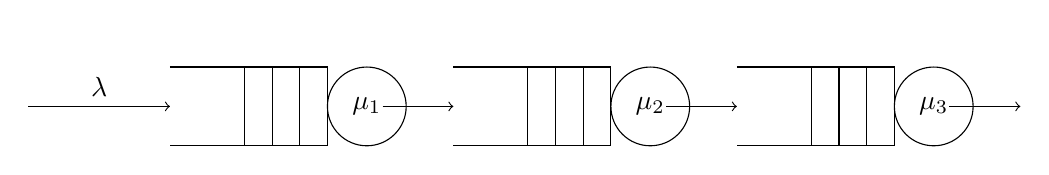
\begin{tikzpicture}[xscale=0.9,
->-/.style={decoration={markings, mark=at position .5 with {\arrow{stealth}}},
postaction={decorate}},
queuei/.pic={
 \draw%[line width=1pt]
 (0,-0.5) -- ++(2cm,0) -- ++(0,-1cm) -- ++(-2cm,0);
 \foreach \Val in {1,...,3}
 \draw ([xshift=-\Val*10pt]2cm,-0.5) -- ++(0,-1cm);
\draw (2.5,-1) circle [radius=0.5cm] node {#1};}
]
\path 
 (0,1) pic {queuei=$\mu_1$}
 (4,1) pic {queuei=$\mu_2$}
 (8,1) pic {queuei=$\mu_3$};

\draw[->] (-2,0)--(0,0) node[midway, anchor=south] {$\lambda$};
\draw[->] (3,0)--(4,0); 
\draw[->] (7,0)--(8,0); 
\draw[->] (11,0)--(12,0); 
%\draw[->-] (2.5,-0.5)-- ++(0,-1) -- ++(5.,0) -- ++(0, 1.5); 

\end{tikzpicture}

\begin{solution} 
 The raw processing time is just the sum of the processing times at
 each station. All stations have the same arrival rate, hence
 machine, being the slowest, is the bottleneck. Hence,
 \begin{align*}
 T_0 &= 2 + 3 + 2 = 7\\
 r_b &= \mu_2 = \frac13 \\
 W_0 &= r_b T_0 = \frac73.
 \end{align*}
\end{solution}
\end{exercise}

\begin{exercise}\clabel{ex:l-203}
 A production network consists of 3 single-machine stations in tandem
 with processing times $(2, 3, 2)$ hours. Suppose we modify this
 network by adding one extra machine to station 2, with processing
 time $t=3$ hours. What are $W_0$, $r_b$ and $T_0$?
\begin{hint}
Is the new machine placed in parallel or in series?
\end{hint}
\begin{solution}
 Realize that machines at a station are in parallel, not in
 series. Thus, when we add capacity to station 2, we don't add an
 extra processing step to station 2, we increase capacity. 

 Now, 
 \begin{equation*}
 r_2 = \frac13 + \frac13 = \frac 23,
 \end{equation*}
 so that station 2 is no longer the bottleneck. Station 1 and
 station 3 are the bottlenecks.
 \begin{align*}
 r_b &= \frac12 \\
 T_0 &= 2 + 3 + 2 = 7\\
 W_0 &= r_b T_0 = \frac72.
 \end{align*}

 Often, students think that the processing rate is the inverse of
 the processing time, i.e., $t=r^{-1}$. This is not the case for
 multi-server stations. Thus, realize that the raw processing time
 at station 2 is still $3$ hours, not $3/2$.
\end{solution}
\end{exercise}


\begin{exercise}\clabel{ex:l-204}
 A production network consists of 3 single-machine stations in tandem
 with processing times $(2, 3, 2)$ hours. Suppose we modify this
 network by adding one extra machine to station 2 with
 processing time $t=4$ hours. What are $W_0$, $r_b$ and $T_0$?
\begin{hint}
Check your reasoning very carefully here. It is easy to do it wrong.
\end{hint}
\begin{solution}
Now, 
\begin{equation*}
 r_2 = \frac13 + \frac 14 = \frac 7{12} > \frac12,
\end{equation*}
hence, station 1 and 3 are bottlenecks. 


However, $t_2$ cannot be $3$ hours anymore: some jobs will spend 4
hours at station 2 rather than 3 hours. In fact, the computation of
the raw processing time at station 2, $t_2$ say, is a bit tricky. Some
students reason that both machines serve half of the jobs, so that
$T_2=(3+4)/2$ hours. This, however, is not quite realistic. Like
this, you would load the slow machine all of the time, and the faster
machine would be idle quite a bit of the time. 


 Rather than spreading the jobs evenly over the two machines, we can
 also assume that each machine takes in work in proportion to its
 processing rate. Then we reason like this. Consider 12 hours. In
 those 12 hours, the slow machine processes 3 jobs with duration 4
 and the fast machine processes 4 jobs with duration 3. Therefore:
 \begin{equation*}
 t_2 = \frac 3 7 4 + \frac 4 7 3 = \frac{24}7.
 \end{equation*}
 Another way to get this is like this. We can `stuff' station 2 with
 jobs. The most jobs that fit in simultaneously is 2, one job per
 machine. Then, with Little's law,
 \begin{equation*}
 t_2 = \frac{W}{r_2} = \frac{2}{7/12} = \frac{24}7,
 \end{equation*}
i.e., the same as the other answer.

Now, finally, 
 \begin{align*}
 r_b &= \frac12 \\
 T_0 &= 2 + \frac{24}7 + 2 = 4 + 3 + \frac37 = 7 \frac37\\
 W_0 &= r_b T_0.
 \end{align*}

 Finally, and the most realistic, is that the fast machine is
 always working, and the slow machine covers the rest. In that
 case, suppose that the fast machine processes jobs at rate $r_1$
 and the slow at rate $r_2$. Then, since jobs arrive with rate
 $r_a$, the fast machine processes a fraction of $r_1/r_a$ of the
 jobs, and the slow machine processes the leftovers, i.e., a
 fraction of $(r_a-r_1)/r_a$ of the jobs. The raw processing time then becomes
 \begin{equation*}
 \begin{split}
 t_2 
&= \frac{r_1}{r_a} t_1 + \frac{r_a-r_1}{r_a} t_2 \\
&= \frac{1/3}{1/2} 3 + \frac{1/2-1/3}{1/2} 4 \\
&= 2 + \frac{1/6}{1/2} 4 \\
&= 2 + \frac{4}{3} = 3\frac13,
 \end{split}
 \end{equation*}
and then,
\begin{equation*}
 T_0 = 2 + t_2 + 2 = 7\frac13,
\end{equation*}
and this is a tiny bit less than the previous way of organizing things. 

So, why are the above answers different? One reason is that the
objective is not explicitly stated. It might be that, to minimize time
in a multi-server station, it is optimal to let a fast machine idle
and wait until the next job comes in. If we were to assign this next
job to a slow machine, the time in the system may be longer. In
general, it might be that schedules that minimize $T_0$ (on average)
are not work-conserving (i.e., such that when jobs are waiting, not
all machines are idle).
\end{solution}
\end{exercise}


\begin{exercise}\clabel{ex:l-205}
Why does the critical WIP change in the different cases above? 
\begin{solution}
 Because $T_0$ increases and/or the bottleneck rate increases. In
 both cases, we need more $W_0$ to fill the network and achieve that
 the throughput can be equal to $r_b$ in the best case.
\end{solution}
\end{exercise}

\begin{exercise}\clabel{ex:l-206}
 A production network consists of 3 single-machine stations in tandem
 with processing times $(2, 3, 2)$ hours. Suppose we modify this
 network by adding one extra machine to station 2 with 
 processing time $t=1$ hour. What are $W_0$, $r_b$ and $T_0$?
\begin{solution}
 Now the slow machine at station 2 becomes superfluous. The fast
 machine at station 2 can cope with all jobs that arrive from station
 1.
 \begin{align*}
 r_b &= \frac12 \\
 T_0 &= 2 + 1 + 2 = 5\\
 W_0 &= r_b T_0.
 \end{align*}

 Thus, why would you assign part of the jobs to the slow machine at
 station 2? There is no queue, the fast machine can cope with all
 the jobs. Moreover, assigning any job to the slow machines just
 adds to the cycle time.

Taking $T_2=(1+3)/2=2$ is plainly silly. 
\end{solution}
\end{exercise}

\begin{exercise}\clabel{ex:l-207}
 In the previous question, it might seem that one machine at the
 second station is superfluous. Which one, and why? Would you remove
 this superfluous machine in a real production network?
\begin{solution}
 See above. I would not remove the slow machine. In real life there
 is variability: the fast machine might fail for instance. Spare
 capacity is useful. However, if it is very costly to keep the slow
 machine operational, I would scrap it.
\end{solution}
\end{exercise}


% What would you have
% said if the processing time of the slow machine would have been 5
% hours? Then you simply cannot give half of the jobs to the slow
% machine; it will overflow.

\begin{exercise}\clabel{ex:l-208}
 A production network consists of 3 single-machine stations in tandem
 with processing times $(2, 3, 2)$ hours. Suppose we modify this
 network by adding one extra machine to station 2 with processing
 time $t=7$ hours. What are $W_0$, $r_b$ and $T_0$?
\begin{solution}
 \begin{align*}
 r_2 &= \frac13 + \frac17 = \frac{10}{21} < \frac12,\\
\intertext{hence station 2 is still the bottleneck}
T_2 &= \frac{3}{10}7 + \frac{7}{10}3 = \frac{42}{10}=\frac{21}{5}\text{hour}\\
T_0&=2+\frac{21}{5} +2\\
r_b &= \frac{10}{21}\\
W_0 &= r_b T_0.
 \end{align*}

 Note that we add capacity, so that we can process more jobs per
 unit time, but the raw processing time increases!
\end{solution}
\end{exercise}


\begin{exercise}\clabel{ex:l-209}
 A production network consists of 3 single-machine stations in tandem
 with processing times $(2, 3, 2)$ hours. Suppose we modify this
 network such that $2/3$ of the jobs \emph{ leave after the first}
 station, i.e., between station 1 and 2. What are $W_0$, $r_b$ and
 $T_0$? 
\begin{solution}
 Now there are two loops. One-third of the jobs pass all three
 stations. Station 1 can process these job at rate 
 \begin{equation*}
\frac13 r_1 = \frac 13 \frac 12=\frac 16
 \end{equation*}
 per hour. Since this is smaller than $r_2$ and $r_3$, station 1 is
 the bottleneck rate for this loop. Thus, $W_0$ in this loop is
 $r_b T_0 = 1/6\cdot 7 = 7/6$.

 The other loop only contains station 1. The bottleneck rate in this
 loop is 
 \begin{equation*}
r_1\frac23 = \frac12\frac23 = \frac13. 
 \end{equation*}
Thus,
 $W_0 = r_b T_0 = 1/3\cdot 2 = 2/3$ for this loop. 

Hence, the total WIP is $7/6 + 2/3 = 11/6$ and
\begin{equation*}
T_0 = \frac13 7 + \frac 23 2=\frac{11}3,
\end{equation*}
since $1/3$ take the long loop with $T=7$ and $2/3$ the short loop
with $T=2$. Thus, $T_0$ is the weighted average raw processing time.

Another way to analyze this situation is like this. Station 1 is the
bottleneck, because its utilization is 1, while
\begin{align*}
 \rho_2 &= \lambda_2 t_2 = \frac12\frac13 3 = \frac 12\\
 \rho_3 &= \lambda_3 t_3 = \frac12\frac13 2 = \frac 13.
\end{align*}
Since station 1 is the bottleneck in this network, $r_b=1/2$. Since
$T_0 = 11/3$, which we obtain as the weighted average computation
above, we must have that 
\begin{equation*}
W_0 = r_b T_0 = \frac12\frac{11}3 = \frac{11}6, 
\end{equation*}
which agrees with our earlier result.
\end{solution}
\end{exercise}


\begin{exercise}\clabel{ex:l-210}
 A production network consists of 3 single-machine stations in tandem
 with processing times $(2, 3, 2)$ hours. Suppose we modify this
 network such that 4/5 of the jobs \emph{bypass the second} station,
 i.e., 1/5 of the jobs have the routing $[1,2,3]$, but 4/5 have
 routing $[1,3]$. What are $W_0$, $r_b$ and $T_0$?
\begin{solution}
 Now stations 1 and 3 are the bottlenecks with $r_b = 1/2$. For $T_0$ we have
 \begin{equation*}
 T_0 = \frac15 7 + \frac45 4= \frac{23}5.
 \end{equation*}
Thus, 
\begin{equation*}
W_0 = r_b T_0 = \frac 12 \frac{23}5 = \frac{23}{10}.
\end{equation*}
\end{solution}
\end{exercise}

\begin{exercise}\clabel{ex:l-211}e}
% Building upon the previous question, which stations would you
% include anyway in a CONWIP loop, and why?
% \end{exercise}
% \begin{solution}
% Now stations 1 and 3 are the bottlenecks. Thus, both stations need to be
% part of the conwip loop. For that matter, it is just as easy to also
% include station 2, and just include all work on the floor in the WIP
% measurements.
% \end{solution}


Production situations can be pretty complicated. Jobs can enter the network at different places, not just at station 1 as we considered here. Jobs may also need rework at one or more stations. One consequence of these aspects is that the slowest machines or stations need not be the bottlenecks. If you like, you can try to find or develop a general algorithm to compute
 $T_0$, $W_0$ and $r_b$ for any network of reasonable size. One way to approach this problem might be to place (imaginary) huge amounts of work in front of each station and just see how the network drains, another is to try to find an analogy with an electrical network. All in all, it's an elegant problem.


\opt{solutionfiles}{
\Closesolutionfile{hint}
\Closesolutionfile{ans}
\subsection*{Hints}
\input{hint}
\subsection*{Solutions}
\input{ans}
}

%\clearpage


%%% Local Variables:
%%% mode: latex
%%% TeX-master: t
%%% End:

%\begin{flalign*}
&\rho = \lambda \frac{\E S}{c} \\
&\E{W_Q} = \frac{C_a^2 + C_s^2}{2} \frac{\rho^{\sqrt{2(c+1)}-1}}{c(1-\rho)} \E S  \\
&\text{Batching: } C_{sB}^2 = \frac{B \V{S_0}+\V{T}}{(B\E{S_0}+\E{T})^2} \\ 
&\text{Nonpreemptive: } \V{S} = \V{S_0} + \frac{\V{T}}{B} + \frac{B -1}{B^2}(\E{T})^2\\
&\text{Preemptive: } A = \frac{m_f}{m_r+m_f}, C_s^2 = C_0^2 + 2A(1-A)\frac{m_r}{\E{S_0}} \\
%& \sigma_s^2 = \sigma_0^2 + \sigma_r^2 f_r + f_r(1-f_r)(\E{S_r})^2 
\\
& C_{di}^2 = 1 + (1-\rho_i^2)(C_{ai}^2 - 1) + \frac{\rho_i^2}{\sqrt{c_i}}(C_{si}^2-1) 
 &\quad 
%C_{ij}^2 = P_{ij}C_{di}^2 + 1 - P_{ij}
\\
& f_i(n_i) = 
            \begin{cases}
              G(i)^{-1} (c_i\rho_i)^{n_i}(n_i!)^{-1}, &\text{ if } n_i < c_i, \\ 
              G(i)^{-1} c_i^{c_i}\rho_i^{n_i}(c_i!)^{-1}, &\text{ if } n_i \geq c_i \\ 
            \end{cases} \\
&\quad \text{with } G(i) = \sum_{n=0}^{c_i-1} \frac{(c_i\rho_i)^n}{n!} + \frac{(c_i\rho_i)^{c_i}}{c_i!}\frac{1}{1-\rho_i} \\
& \E{L_i} = \frac{(c_i\rho_i)^{c_i}}{c_i!G(i)}\frac{\rho_i}{(1-\rho_i)^2} + c_i \rho_i &\quad
% C_{si}^2 = \max\{C_{si}^2, 0.2\} 
\\
%& Q_{ij} = \frac{\lambda_{ij}}{\lambda_j}, i=0\ldots M, j=1\ldots M &\quad C_{aj}^2 = w_j\sum_{i=0}^M Q_{ij}C_{ij}^2 + 1 - w_j \\
%& w_j = (1+4(1-\rho_j)^2(v_j-1))^{-1} &\quad 
% v_j = \left(\sum_{i=0}^M Q_{ij}^2\right)^{-1}, \, j=1,\ldots, M,\\
& f_{i}(n_i) = \frac{1}{\Pi_{k=1}^{n_i} \min\{k, c_i\}}\left(\frac{V_i}{\mu_i}\right)^{n_i}, i=0\ldots M \\
& V_i = (V P)_i = \sum_{j=0}^M V_j P_{ji}\\
%& G(m,n) = \sum_{k=0}^n f_m(k) G(m-1, n-k) &\quad  G(m,0) = 1, G(0,n) = \mu_0^{-n}, \\
%& \E{W_j(n)} = \E{L_j(n-1) + 1} \E{S_j} &\quad \E{L_j(n)} = \TH_j(n) \E{W_j(n)} \\
%& \TH_0(n) = \frac{n}{\sum_{j=0}^M V_j \E{W_j(n)}}  &\quad  \TH_j(n) = V_j \TH_0(n) \\
%&  p_j(0|0) = 1  &\quad \E{W_j(n)} = \sum_{k=c_j}^{n-1} \frac{k-c_j+1}{c_j \mu_j} p_j(k|n-1) + \frac{1}{\mu_j} \\
%& p_j(k|n) = \frac{\TH_j(n)}{\mu_j \min\{c_j,k\}} p_j(k-1|n-1), k=1\ldots N &\quad p_j(0|n) = 1 - \sum_{k=1}^n p_j(k|n).
\end{flalign*}



\section{Open Single-Class Product-Form Networks}
\label{sec:jackson-networks}


\subsection*{Theory and Exercises}

\Opensolutionfile{hint}
\Opensolutionfile{ans}

The remark above Zijm.Eq.2.11 is not entirely correct. Remove the
sentence: `These visit ratios satisfy \ldots up to a multiplicative
constant'.


I don't like the derivation of Zijm.Eq.2.20. The appearance of the
visit ratios $\lambda_i/\gamma$ seems to come out of thin air. The
argument should be like this. Consider the entire queueing network as
one `box' in which jobs enter at rate $\gamma=\sum_{i=1}^M
\gamma_i$.
Assuming that there is sufficient capacity at each station, i.e.,
$\lambda_i < c_i \mu_i$ at each station $i$, the output rate of the `box' must also be $\gamma$. Thus, by applying Little's law to the `box', we have that 
\begin{equation*}
  \E L = \gamma \E W. 
\end{equation*}
It is also evident that the average total number of jobs must be equal
to the sum of the average number of  jobs at each station: 
\begin{equation*}
  \E L = \sum_{i=1}^M \E{L_i}.
\end{equation*}
Applying Little's law to each station separately we get that
$\E{L_i} = \lambda_i\E{W_i}$. Filling this into the above,
\begin{equation*}
\E W = \frac{\E L}{\gamma}  = \sum_{i=1}^M \frac{\E{L_i}}\gamma = \sum_{i=1}^M \frac{\lambda_i \E{ W_i}}\gamma, 
\end{equation*}
where we recognize the visit ratios.




\begin{comment}
\begin{exercise}[use=false]
  Use the ideas of Zijm.Eq.2.2 to set up a set of balance equations
  for a single-server queueing station with two queues such that queue
  1 is served with strict priority over queue 2, and service of a job
  of type 2 is preemptive. Assume that type i jobs arrive at rate
  $\lambda_i$ and require average service time
  $\mu_i^{-1}$. Inter-arrival times of jobs each type are exponentially distributed,
  just as the service times.

  Can you find similar equations for the case with multiple servers at
  the station, all serving type 1 jobs with strict priority over type
  2 jobs?
  \begin{solution}
    TBD.
  \end{solution}
\end{exercise}
  
\end{comment}

\begin{exercise}(Linear algebra refresher) Can you find an example to
  show for two matrices $A$ and $B$ that $AB\neq BA$, hence
  $x A \neq A x$.
  \begin{hint}
    Let 
    \begin{equation*}
A =
    \begin{pmatrix}
      1 & 1 \\ 
0&1
    \end{pmatrix},
\quad   B=
    \begin{pmatrix}
      1 & 0 \\ 
1&1
    \end{pmatrix}.
    \end{equation*}
  \end{hint}

  \begin{solution}
    \begin{equation*}
      AB =  
    \begin{pmatrix}
      2 & 1 \\ 
1&1
    \end{pmatrix} 
\neq
    \begin{pmatrix}
      1 & 1 \\ 
1&2
    \end{pmatrix} 
= BA.
    \end{equation*}

Take $x=(1,1)$, then $x A=(1,2)$. Now, taking $x=
\begin{pmatrix}
  1 \\
1
\end{pmatrix}
$, we get $Ax = 
\begin{pmatrix}
  2 \\
1
\end{pmatrix}.  $
Recall, horizontal vectors are not vertical vectors. The horizontal
ones are to the left of a matrix, and the vertical ones to the right.
  \end{solution}
\end{exercise}

\begin{exercise}(Linear algebra refresher, 2) Suppose the matrix $A$
  has an eigenvalue $0$. What is the geometric meaning of this fact? 
  \begin{solution}
    Many students think that a matrix is just a bunch of numbers
    ordered in a grid. This is, in my opinion, the most unproductive
    way to think about matrices. A much more useful way is to see a
    matrix as an \emph{operator}. For instance, take $A$ to be a
    $3\times3$ matrix. Then it can be seen as a \emph{mapping} from
    $\R^3$ to $\R^3$; it takes a vector $x\in\R^3$ and changes $x$
    into a new vector $Ax\in \R^3$. Thus, a square matrix $A$ typically changes the
 direction of a vector $x$. 

With this idea, consider the simple example with
    \begin{equation*}
A =
    \begin{pmatrix}
      1 & 0 & 0 \\ 
      0 & 1 & 0 \\ 
      0 & 0 & 0 \\ 
    \end{pmatrix}.
  \end{equation*}
Clearly, $A$ has an eigenvalue $0$. Now take $v=(x,y,z)'$, so that
    \begin{equation*}
A v = A
 \begin{pmatrix}
x\\
y\\
z
    \end{pmatrix}
= \begin{pmatrix}
x\\
y\\
0
    \end{pmatrix}.
  \end{equation*}
  We see that $A$ removes any information about the $z$ direction from
  the vector $v$. (It projects $v$ on the $x-y$ plane, and throws away
  the $z$ component of $v$.) But then, for a given vector $w=(x,y,0)$
  in the $x-y$ plane, it is impossible to use $A$ to retrieve the
  original vector $v=(x,y,z)$. Thus, $A$ cannot have an inverse on all
  of $\R^3$.

  So, hopefully, with this example, you can memorize that for any
  matrix $A$ to have an inverse, it is essential that it has no zero
  eigenvalues. When the \emph{operator} $A$ (don't think of a matrix
  as a set of numbers) throws away part of the dimension of the space
  on which it operates (i.e., it has one or more eigenvalue(s) $0$), it is impossible to retrieve the part of the space it throws away. Hence, its inverse cannot be used to get this part of the space back. 

\end{solution}


\end{exercise}


\begin{exercise}
Zijm.Ex.2.2.1
\begin{solution}
Because jobs cannot leave faster than they arrive.
\end{solution}
\end{exercise}

\begin{exercise}
Zijm.Ex.2.2.2
\begin{solution}
  Observe from Exercise~\ref{ex:dep} that the inter-departure times
  of the $M/M/1$ queue are also independent and identically
  exponentially distributed with rate $\lambda$. Since the arrival
  process at the second station is the departure process of the first
  station, it must be that arrival process at the second station is
  also Poisson with rate $\lambda$.  Interestingly, from the
  perspective of the second station it is as if there is no first
  station.
\end{solution}
\end{exercise}



\begin{exercise}
Zijm.Ex.2.2.3 
\begin{solution}
  The question is not well specified. We know from Burke's law, see Exercise~\ref{ex:burke}, that
  the arrival \emph{process} at the second station is Poisson.  If,
  however, we know that station 1 is empty, then it is unlikely that a
  job will arrive at station 2 in the very near future.

  Note that only the steady-state distributions of the queue lengths
  are independent. Once you have information about the state of one of
  the queues, then certainly this is not in `steady-state'.
\end{solution}
\end{exercise}

\begin{exercise}
Zijm.Ex.2.2.4
\begin{solution}
  Simple algebra.  (I am not going to write it out here. If you are
  willing to provide me the answer in \LaTeX\/ I'll include it.)
\end{solution}
\end{exercise}

\begin{exercise}
  Zijm.Ex.2.2.5. The problem is not entirely correctly formulated. It
  should be, if for at least one $i$, $\sum_{j=1}^M P_{i j} <1$ \ldots
\begin{solution}
Linear algebra is quite useful here!

Observe that $P_{i j}$ is the probability that a job, after completing
its service at node $i$, moves to node $j$. Then $\sum_{j=1}^M P_{i j}$
is the probability that a job moves from node $i$ to another node in
the network, i.e., stays in the network, while $P_{i0}$ is the
probability that a job departing from node $i$ leaves the network, in
other words, the job is finished. When $\sum_{j=1}^M P_{i j} < 1$, then
more jobs enter node $i$ from the network than that node $i$ sends
`back' into the network. Conceptually, node $i$ `leaks jobs'.

  Now, consider some node $k$ such that $P_{ki} > 0$, then the
  probability that a job that starts at node $k$, moves to node $i$
  and then leaves the network is equal to $P_{ki}P{i0}$. Thus, since
  $P_{ki}>0$ and $P_{i0}>0$, the probability that a job leaves the
  network from note $k$ in two steps is positive.  More specifically,
  $P^2_{k0} = \sum_{j=0}^M P_{kj}P_{j0} \geq P_{ki}P_{i0} > 0$. 

  The irreducibility assumption implies that in at most $M$ steps it
  is possible to reach, with positive probability, any node from any
  other node in the network. Thus, for any node $j$ to any other node
  $k$ there is a sequence of nodes $j_1, j_2, \ldots, j_{M-1}$ such
  that  $P^{M}_{jk} \geq P_{j j_1}P_{j_1 j_2}\cdots P_{j_{M-1}k} > 0$.


  Thus, if there is a node $i$ such that $P_{i0}>0$, then it is
  possible from any node that sends jobs to node $i$ directly to leave
  the network in two steps. Likewise, when node $i$ can be reached
  from node $k$ in $n$ steps, say, then
  $P^{n+1}_{k0} \geq P^n_{ki}P_{i0} > 0$, i.e., in at most $n+1$ steps
  it is possible to leave the network from such node $k$. This
  implies, in particular, that for all nodes $k=1,2,\ldots, M$, i.e.,
  all nodes in the network, $P^{M+1}_{k0} >0$.  For this reason we
  consider $P^{M+1}$ in the hint.


  As a final remark for students with knowledge of Markov chains,
  observe that the routing matrix $P$ does not correspond to the
  transition matrix of a recurrent Markov chain. Since for at least
  one row $i$, $\sum_{j=1}^N P_{i j}<1$, the matrix $P$ is
  sub-stochastic. Hence, a Markov chain induced by $P$ cannot be
  irreducible, because for this to happen, the chain must stay in some
  absorbing set with probability 1.
\end{solution}
\end{exercise}

\begin{exercise}\label{ex:20}
Zijm.Ex.2.2.6
\begin{solution}
  Since $M$ is finite, and $k\leq M$, the set of numbers
  $P^{M+1}_{k0}$ is finite. This, together with the fact that
  $P^{M+1}_{k0}>0$ for all $k$, implies that there is some number
  $\epsilon>0$ such that $P^{M+1}_{k0}>\epsilon$. Hence, for all
  entries $k=1, 2, \ldots, M$, we have that
  $P^{M+1}_{kj} < 1- \epsilon$. This, in turn, implies that
  $P^{2(M+1)}_{kj} < (1- \epsilon)^2$, and so on, so that for any $n$,
  $P^{n(M+1)}_{kj} < (1- \epsilon)^n$. This implies, in more general
  terms, that the entries of $P^n$ decrease at some geometric rate to
  $0$.

  It is well known that for any bounded sequence $x_i$ and
  $0\leq \alpha < 1$, $ \sum_{i=0}^\infty x_i \alpha^i <
  \infty$. Applying this insight to the entries of $P^n$ it follows that 
$\sum_{n=0}^\infty P^n_{jk} < \infty$. 

Finally, applying  $\lambda = \gamma + \lambda P$ recursively, we get
\begin{equation*}
  \lambda = \gamma + \lambda P = \gamma + (\gamma + \lambda P)P = \gamma (1+P) + \lambda P^2 = \gamma(1+P+P^2) + \lambda P^3 \to \gamma \sum_{n=0}^\infty P^n.
\end{equation*}
By the above reasoning this last sum is well defined, and finite.  (By
the way, the above argument is not necessarily valid for matrices $P$
that are infinite, since then $\inf\{P^{M}_{ik}\}$ need not be
strictly positive.)

Another interesting way to see all this is by making the simplifying
assumption that $P$ is a diagonalizable matrix. (The argument can be
generalized to include matrices reduced to Jordan normal form, but
this gives optimal clutter, but does not change the line of reasoning in
any fundamental way.) In that case, there exists an invertible matrix
$V$ with the (left) eigenvectors of $P$ as its rows and a diagonal
matrix $\Lambda$ with the eigenvalues on its diagonal such that
\begin{equation*}
  V P = \Lambda V.
\end{equation*}
Hence, premultiplying with $V^{-1}$, 
\begin{equation*}
  P = V^{-1}\Lambda V.
\end{equation*}
But then
\begin{equation*}
P^2 = V^{-1}\Lambda V \cdot V^{-1}\Lambda V= V^{-1}\Lambda^2 V,
\end{equation*}
and in general $P^n = V^{-1}\Lambda^n V$.
If each eigenvalue $\lambda_i$ is such that its modulus $|\lambda_i| < 1$, then $\Lambda^n \to 0$ geometrically fast, hence $P^n\to 0$ geometrically fast, hence the sequence of partial sums $\sum_{n=0}^N P^n$ converges to a matrix with finite elements as $N\to\infty$.

So, we are left with proving that the eigenvalues of $P$ must have
modulus less than $1$. This fact follows from Gerschgorin's disk
theorem, which I include for the interested student. Define the disk
$B(a,r)=\{z\in \mathbb{C} | |z-a|\leq r\}$, i.e., the set of complex numbers
such that the distance to the center $a\in \mathbb{C} $ is less than or equal
to the radius $r$. With this, the Gerschgorin disks of a matrix are
defined as $B(a_{ii}, \sum_{j\neq i} |a_{i j}|)$, i.e., disks with
center at the diagonal elements $a_{ii}$ of $A$ and radius equal
to the sum of the (modulus of the) elements of $A$ on the $i$th row
except $a_{ii}$. Then Gerschgorin's theorem says that all eigenvalues
of $A$ lie in the union of these disks, i.e., all eigenvalues
$\lambda_i \in \bigcup_i B({a_{ii}, \sum_{j\neq i}|a_{i j}})$.

Assume for notational simplicity that for each row $i$ of $P$ we have
that $\sum_{j} a_{i j}<1$. (Otherwise apply the argument to $P^{M+1}$.)
Then this implies for all $i$ that
\begin{equation*}
  a_{ii} + \sum_{j\neq i} a_{i j} < 1. 
\end{equation*}
Since all elements of $P$ are non-negative, this also implies that
\begin{equation*}
-1 <   a_{ii} - \sum_{j\neq i} a_{i j} \leq  a_{ii} + \sum_{j\neq i} a_{i j} < 1. 
\end{equation*}
With this and using that $a_{ii}$ is a real number (so that it lies on
the real number axis) it follows that all elements in the disk
$B(a_{ii}, \sum_{j\neq i} a_{i j})$ have modulus smaller than 1.  As
this applies to any row $i$, all disks lie strictly within the complex
unit circle. But then, by Gerschgorin's theorem, all eigenvalues of
$P$ also lie strictly in the unit circle, hence all eigenvalues have
modulus smaller than 1.
\end{solution}
\end{exercise}

\begin{exercise}\label{ex:23}
  Show that Zijm.Eq.2.13 and 2.14 can be written as
  \begin{equation*}
    f_i(n_i) = \frac{1}{G(i)}\frac{1}{\Pi_{k=1}^{n_i} \min\{k, c_i\}}\left( \frac{\lambda_i}{\mu_i}\right)^{n_i}.
  \end{equation*}
  \begin{solution}
    Take $n_i<c_i$. Then
    $\Pi_{k=1}^{n_i} \min\{k, c_i\} = \Pi_{k=1}^{n_i} k = n_i!$, and
    $(c_i\rho_i)^{n_i} = (\lambda_i/\mu_i)^{n_i}.$ If $n_i\geq c_i$,
    then $\Pi_{k=1}^{n_i} \min\{k, c_i\} = c_i! c_i^{n_i-c_i}$, and
    $(c_i\rho_i)^{n_i} = (\lambda_i/\mu_i)^{n_i} c_i^{n_i}$.
  \end{solution}
\end{exercise}


\begin{exercise}
Zijm.Ex.2.2.7
\begin{solution}
  \begin{equation*}
    P = 
    \begin{pmatrix}
      \alpha & 1- \alpha \\
      \beta_1 & \beta_2
    \end{pmatrix}.
  \end{equation*}

  \begin{equation*}
    (\lambda_1, \lambda_2) = (\gamma, 0) + (\lambda_1, \lambda_2) P.
  \end{equation*}
Solving first for $\lambda_2$ leads to $\lambda_2 = (1-\alpha) \lambda_1 + \beta_2 \lambda_2$, so that  
\begin{equation*}
  \lambda_2 = \frac{1-\alpha}{1-\beta_2} \lambda_1. 
\end{equation*}
Next, using this and that $\lambda_1 = \alpha \lambda_1 + \beta_1 \lambda_2 + \gamma$ gives with a bit of algebra
\begin{equation*}
  \begin{split}
\gamma 
&=  \lambda_1(1-\alpha) - \beta_1\lambda_2 \\
&=  \lambda_1\left(1-\alpha - \beta_1\frac{1-\alpha}{1-\beta_2}\right) \\
&=  \lambda_1(1-\alpha)\left(1 - \frac{\beta_1 }{1-\beta_2}\right) \\
&=  \lambda_1(1-\alpha)\frac{1-\beta_1-\beta_2 }{1-\beta_2}.
  \end{split}
\end{equation*}
Hence, 
\begin{equation*}
  \lambda_1 = \frac\gamma{1-\alpha}\frac{1-\beta_2}{1-\beta_1-\beta_2}. 
\end{equation*}
Thus, 
\begin{equation*}
  \lambda_2 = \frac{1-\alpha}{1-\beta_2} \lambda_1 = \frac\gamma{1-\beta_1-\beta_2}. 
\end{equation*}


We want of course that $\lambda_1 < \mu_1$ and $\lambda_2 < \mu_2$.
With the above expressions this leads to conditions on $\alpha$,
$\beta_1$ and $\beta_2$. Note that we have three parameters, and two
equations; there is not a single condition from which the stability
can be guaranteed.

If $\alpha\uparrow 1$, the arrival rate at node $1$ explodes. If
$\beta_1=0$ no jobs are sent from node 2 to node 1.

\end{solution}
\end{exercise}
\begin{exercise}
Zijm.Ex.2.2.8
\begin{solution}
  Yes, the network remains a Jackson network. By Burke's law, see Exercise~\ref{ex:burke}, the
  departure process of each node is Poisson. In one of the earlier
  questions we derived that splitting (also known as thinning) and
  merging Poisson streams again lead to Poisson streams. The
  departures from node $j$ to node $k$ forms a thinned Poisson
  stream. The external arrivals plus internal arrivals are merged into
  one Poisson stream, hence the arrivals at a station also form a Poisson stream.

  Observe that the exponentiality of the service times and external
  inter-arrival times and Burke's law are essential for the argument.
\end{solution}
\end{exercise}

\begin{exercise}
  (Hall 5.22). At a large hotel, taxi cabs arrive at a rate of 15 per
  hour, and parties of riders arrive at the rate of 12 per
  hour. Whenever taxicabs are waiting, riders are served immediately
  upon arrival. Whenever riders are waiting, taxicabs are loaded
  immediately upon arrival. A maximum of three cabs can wait at a time (other cabs must go elsewhere).
  \begin{enumerate}
  \item Let $p_{ij}$ be the steady-state probability of there being $i$ parties of riders and $j$ taxicabs waiting at the hotel. Write the state transition equation for the system. 
  \item Calculate the expected number of cabs waiting and the expected number of parties waiting.
  \item Calculate the expected waiting time for cabs and the expected waiting for parties. (For cabs, compute the average among those that do not go elsewhere.)
  \item In words, what would be the impact of allowing four cabs to wait at a time?
  \end{enumerate}
  \begin{hint}
This is really a neat problem. Please spend serious time on it to
solve before looking at the answer. It requires some ingenuity on your part.  Try to adapt the ideas behind Figure 2.2 of Zijm to this case.
  \end{hint}
    \begin{solution}
Let $p_{ij}$ be the fraction of time that the system contains $i$
riders and $j$ taxi cabs. I assume that all members of a party of
riders can be served by a single cab (that is, the parties do not
exceed the capacity of a cab and all members of a party have the same
destination). For clarity, write $\mu$ for the rate at which cabs
arrive, and $\lambda$ for the arrival rate of parties of riders.  Then
the transitions are as in the figure below. Suppose first that there
are $3$ taxi cabs. When a group arrives (at rate $\lambda$), there is
one taxi less, and so on, until there are no more taxis
left. Finally, if yet more groups arrive, they have to wait. When a
new taxi arrives, the number of groups is reduced by one, and so on,
until there are $3$ taxis waiting and no groups of people.


    \begin{center}

\begin{tikzpicture}[->,>=stealth',shorten >=1pt,auto,node distance=1.8cm,
                    semithick]
  \node[state] (0) {$p(0,3)$} ;
  \node[state] (1) [right of=0] {$p(0,2)$};
  \node[state] (2) [right of=1] {$p(0,1)$};
  \node[state] (3) [right of=2] {$p(0,0)$};
  \node[state] (4) [right of=3] {$p(1,0)$};
  \node[state] (5) [right of=4] {$p(2,0)$};
  \node[state] (6) [right of=5] {$p(\cdot, 0)$};

\path 
 (0) edge [bend left] node {$\lambda$} (1)
 (1) edge [bend left] node {$\mu$} (0)
 (1) edge [bend left] node {$\lambda$} (2)
 (2) edge [bend left] node {$\mu$} (1)
 (2) edge [bend left] node {$\lambda$} (3)
 (3) edge [bend left] node {$\mu$} (2)
 (3) edge [bend left] node {$\lambda$} (4)
 (4) edge [bend left] node {$\mu$} (3)
 (4) edge [bend left] node {$\lambda$} (5)
 (5) edge [bend left] node {$\mu$} (4)
 (5) edge [bend left] node {$\lambda$} (6)
 (6) edge [bend left] node {$\mu$} (5)
;
\end{tikzpicture}
      
    \end{center}

From this figure, we see that
\begin{align*}
\lambda p_{0,3} &= \mu p_{0,2} \\
(\lambda+\mu) p_{0,2} &= \mu p_{0,1} + \lambda p_{0,3}\\
(\lambda+\mu) p_{0,1} &= \mu p_{0,0} + \lambda p_{0,2}\\
(\lambda+\mu) p_{0,0} &= \mu p_{1,0} + \lambda p_{0,1}\\
(\lambda+\mu) p_{1,0} &= \mu p_{2,0} + \lambda p_{0,0}\\
(\lambda+\mu) p_{2,0} &= \mu p_{3,0} + \lambda p_{1,0}\\
\end{align*}
and so on. Thus, it is left to compute $p_{ij}$. Observe from this
scheme, or the above figure, that the situation with the taxi's
correspond to an $M/M/1$ queue, only the states have a `different
name'. Let $q$ be the number of jobs in an M/M/1 queue. Some thought
will reveal that the queueing system with cabs and parties can be
mapped to an equivalent M/M/1 queueing system. In fact, consider the
following table
\begin{center}
\begin{tabular}{ccc}
$j$ & $i$ & $q$\\
3&         0 &         0\\
2 &        0&          1\\
1 &        0&          2\\
0&         0&          3\\
0&         1&          4\\
0&         2&          5\\
\end{tabular}
\end{center}
and so on. Therefore, in general, it must be that 

\begin{equation*}
q = 3 - j +i.
\end{equation*}
From the M/M/1 queue we know right away that $p_q = \rho^q
(1-\rho)$.  With the above relation we can therefore immediately find
that $p_{ij} = \rho^{3-j+i}(1-\rho)$, save that $i$ and
$j$ must satisfy the constraints imposed by the model.

Second, the expected number of cabs waiting must be 
\begin{equation*}
1p_{0,1} + 2 p_{0,2} + 3p_{0,3}
\end{equation*}
and the expected number of parties waiting must be $\sum_{j=1}^\infty j p_{j,0}$.

\begin{pyconsole}
labda = 12. # per hour
mu = 15. # per hour
rho = labda/mu

def p(i,j):
    q  = 3 - j + i
    return rho**q*(1.-rho)

\end{pyconsole}
Expected number of  cabs waiting:
\begin{pyconsole}
Lc = sum(j*p(0,j) for j in range(0,4)) 
# Recall this sums up to 4, not including 4
Lc
  
\end{pyconsole}


To compute the expected number of parties waiting we formally have to
sum to infinity. Rather than doing the algebra, I chose to truncate
the summation at an $i$ such that $\rho^i \ll 1$, i.e.,
negligible.  Truncating at 30 seems reasonable enough:

\begin{pyconsole}
trunc = 30
rho**trunc
\end{pyconsole}

At second thought this is not yet really small. 

\begin{pyconsole}
trunc = 50
rho**trunc
\end{pyconsole}


This is better. Now go for what we want to know:

\begin{pyconsole}
Lp = sum(i*p(i,0) for i in range(trunc))
Lp
\end{pyconsole}

For the last part: This is tricky. I first, naively, computed $W_q = L_c/\mu$. This
seems to make sense, as cabs arrive at rate $\mu$, so that this
expression follows from a standard application of Little's
law. However, this is wrong, of course. When using Little's law to
relate the number of jobs in queue (i.e., in the M/M/1 queue) and the
queueing time we need to use $\lambda$, not
$\mu$. Similarly (and more formally by the mapping developed in
part a), for our cab system we also need to use $\lambda$.

\begin{pyconsole}
Wq = Lc/labda
Wq
\end{pyconsole}

Thinking in templates is often useful, but makes one sloppy\ldots

What would be the impact of allowing 4 cabs? Funny question, and with the above, trivial to answer.

\begin{pyconsole}
def p(i,j):
    q  = 4 - j + i
    return rho**q*(1.-rho)
  
\end{pyconsole}

\begin{pyconsole}
Lc = sum(j*p(0,j) for j in range(0,4))
Lc

Lp = sum(i*p(i,0) for i in range(trunc))
Lp
  
\end{pyconsole}
    \end{solution}
\end{exercise}



\begin{comment}
  
\begin{exercise}[use=false]
  Include an question that shows that it is necessary to check the
  guess for the product form solution everywhere on the state space,
  that is, in the interior, but also on the boundaries.
  \begin{solution}
    TBD
  \end{solution}
\end{exercise}

\begin{exercise}[use=false]
  Apply the formula's of Zijm.Section 2.4 to a tandem queueing network.
  \begin{solution}
    TBD.
  \end{solution}
\end{exercise}

\begin{exercise}[use=false]
  Include a case for Section 2.4.
  \begin{solution}
    TBD.
  \end{solution}
\end{exercise}
\end{comment}


\Closesolutionfile{hint}
\Closesolutionfile{ans}

\opt{solutionfiles}{
\subsection*{Hints}
\input{hint}
\subsection*{Solutions}
\input{ans}
}
%\clearpage



%%% Local Variables:
%%% mode: latex
%%% TeX-master: "../queueing_book"
%%% End:

%
\section{Gordon-Newell Networks}
\label{sec:gordonNewell}


\subsection*{Theory and Exercises}

\Opensolutionfile{hint}
\Opensolutionfile{ans}


\begin{exercise}
  Provide an interpretation of a single-server queueing server with a
  finite calling population in terms of a closed network.
\begin{solution}
    Consider a closed-queueing network with two stations. Station 1 is
    a single-server station with exponentially distributed service
    times with mean $\mu$; station 2 has $N$ parallel exponential
    servers, each working at rate $\lambda$. If station 1 contains $n$
    jobs, then Station 2 contains $N-n$ jobs.  The rate at which jobs
    move from Station 2 to Station 1 is $(N-n)\lambda$, since $N-n$ of
    the $N$ servers of Station 2 are occupied. Jobs move from Station
    1 to Station 2 at rate $\mu$, provided $n\geq1$.
  \end{solution}
\end{exercise}

The formula with the visit ratios should be like this:
\begin{equation*}
  V_k = \sum_{j=0}^M V_j P_{jk}, 
\end{equation*}
i.e., the sum should start at index 0. This is to include the
load/unload station.

Also, assume that the load/unload station has just one server.

% It is perhaps the easiest to start with studying the MVA algorithm,
% then the MDA algorithm and finish with the convolution algorithm.

You should realize that the algorithms discussed in this section are
meant to be carried out by computers. Thus the results will be
numerical, not in terms of formulas.

Mind the order of $V$ and $P$ in the computation of the visit ratios:
do not mix up $VP=V$ with $P V=V$, as in general, $VP \neq P V$.  We use
$VP=V$.


\begin{exercise}\label{ex:mva}
  Compute the visit ratios for a network with three stations such that all jobs from station 0 move to station 1, from station 1 all move to station 2, and from station 2 half of the jobs move to station 0 and the other half to station 1. 
  \begin{solution}
    The routing matrix $P$ is
    \begin{equation*}
      P = 
      \begin{pmatrix}
        0 & 1 & 0 \\
0& 0 & 1 \\
1/2 & 1/2 & 0
      \end{pmatrix}.
    \end{equation*}
    Solving $V=VP$ leads to
    $(V_0, V_1, V_2) = (V_2/2, V_0 + V_2/2, V_1)$. Thus, from the last
    item, $V_2 = V_1$, and from the first $V_0 = V_2/2$. Since
    $V_0=1$, it follows that $V_2 = 2V_0$ and $V_1=V_2=2 V_0$.
  \end{solution}
\end{exercise}

\begin{exercise}
Zijm.Ex.3.1.1 
\begin{solution}
If a part would need refitting or repositioning at the load/unload station, then that part would visit the load/unload station more than once during its stay in the network. The visit ratio of the load/unload station can then no longer be set to 1.
\end{solution}
\end{exercise}

\begin{exercise}
Zijm.Ex.3.1.2
\begin{solution}
Let's number the states from 1 to 4. If station 1 feeds into station 2, and so on, and station 4 into station 1, then 
\begin{equation*}
  P = 
  \begin{pmatrix}
    0 & 1 & 0 & 0\\
    0 & 0 & 1 & 0\\
    0 & 0 & 0 & 1\\
    1 & 0 & 0 & 0\\
  \end{pmatrix}.
\end{equation*}
The visit ratios are, of course, $V_1= V_2 = V_3 = V_4$. 
\end{solution}
\end{exercise}

\begin{exercise}
Zijm.Ex.3.1.3
\begin{solution}
We number  station a as 1, and so on.
\begin{equation*}
  P = 
  \begin{pmatrix}
     0 & 1 & 0 & 0 & 0 &0 \\
     1/5 & 0 & 4/5 & 0 & 0 & 0\\
     0& 0 & 0 & 1/3 & 2/3 & 0 \\
     0 & 0 & 0 & 0 & 0 & 1\\
     0 & 0 & 0 & 0 & 0 & 1\\
     1 & 0 & 0 & 0 & 0 & 0\\
  \end{pmatrix}.
\end{equation*}
We now solve for $V$ in the equation $V = VP$.
Since, by definition, node $f$ is the load/unload node, we set $V_6=1$, and then we express the other visit ratios in terms of $V_6$.
Note also that the rows of $P$ sum up to one.
Hence, From elementary linear algebra, the second column implies that $V_2 = V_1$, and the third that $V_3 = 4/5 \cdot V_2$, so that $V_3 = 4/5 \cdot V_1$.
From the fourth column $V_4 = V_3 \cdot 1/3 $, thus, $V_4 = V_1 \cdot 1/3 \cdot 4/5 = V_1 \cdot 4/15$.
From the fifth column $V_5 = V_3 \cdot 2/3$, hence $V_5 = V_1 \cdot 4/5 \cdot 2/3 = V_1 \cdot 8/15$.
Finally, from the sixth column, $V_6 = V_4+V_5$, hence $V_6 = V_1 (4/15 + 8/15)=V_1 \cdot 4/5$.
Therefore, $V_1 = V_6 \cdot 5/4$.
Then using $V_6 = 1$ and the above obtained results give $V_1 = V_2 = 5/4$, $V_3 = 1$, $V_4 = 1/3$, and $V_5 = 2/3$.

(Note that this also could be derived from the first column and the second colum, i.e., since $V_1 = 1/5 \dot V_2 + V_6$ and $V_2 = V_1$, rewriting gives, $V_1 = 1/5 \dot V_2 + V_6 = V_1 = 1/5 \cdot V_1 + V_6$ which gives $4/5 \cdot V_1 = V_6$ and hence $V_1 = 5/4 \cdot V_6$.)

For later courses on Markov chains, it is important to note the following.
Write the visit ratio equation $V = VP$ as $V(1-P)=0$ where $1$ is the indicator matrix.
Clearly, $V$ is a left eigenvector of the matrix $1-P$ with eigenvalue 0 (recall that $V(1-P) = 0 = 0\cdot V$).
Thus, at least one row or column of the matrix $1-P$ is superfluous to solve for $V$.
\end{solution}
\end{exercise}

\begin{exercise}
  Relate Zijm.Eq.3.3 to the form of the steady-state distribution of
  the number of jobs in an $M/M/c$ queue.
  \begin{solution}
    Except for the normalization constant, the expressions are the
    same as equations 1.36 and 1.37 of Zijm's book.
  \end{solution}
\end{exercise}

\begin{exercise}
Zijm.Ex.3.1.4
\begin{solution}
Consider network one with routing $1\to3\to4\to2\to1$, each transition occurring with probability one, i.e.,
\begin{equation*}
  P =
  \begin{pmatrix}
    0 & 0 & 1 & 0  \\
    1 & 0 & 0 & 0  \\
    0 & 0 & 0 & 1  \\
    0 & 1 & 0 & 0  \\
  \end{pmatrix}.
\end{equation*}
All nodes are is visited equally often. Another network could correspond to the routing $1\to2\to3\to4\to1$.  Yet another would be this:
\begin{equation*}
  P =
  \begin{pmatrix}
    1/2 & 0   & 1/2 & 0  \\
    1/2 & 1/2 & 0 & 0  \\
    0   & 1/2 & 0 & 1/2  \\
    0   & 0   & 1/2 & 1/2  \\
  \end{pmatrix}.
\end{equation*}
Observe that I choose the rate such that each node receives the same
fraction of traffic.

For the interested: There must be many such `equivalent' networks, but
a general method to classify all equivalent networks seems hard. The
question comes down to finding all stochastic matrices $P$ that have
at least one (left) eigenvector $V$ in common. Observe that the visit
ratio equation $VP=V$ implies that $V$ is a left eigenvector with
eigenvalue 1.
\end{solution}
\end{exercise}

\begin{exercise}
Zijm.Ex.3.1.5
\begin{hint}
 First write down all  different states, and then use Zijm.Eq.3.2 and 3.3.
\end{hint}
\begin{solution}
  Since $M=2$, we have three stations: Stations 0, 1, and 2. We also
  have $N=2$ jobs. Thus, the states are $(2,0,0)$ (meaning that the
  load/unload station has 2 jobs, and stations 1 and 2 no jobs),
  $(0,2,0)$, $(0,0,2)$, $(1,1,0)$, $(1,0,1)$, and $(0,1,1)$. Note that
  the routing matrix $P$ is not given, so that we cannot compute the
  visit ratios. Hence I leave them unspecified. Now, realize that for
  a fixed $\vec n=(n_0, n_1, n_2)$,
  $\Pi_i f_i(n_i) = f_0(n_0)f_1(n_1)f_2(n_2)$, so that if 
  \begin{align*}
    \vec n &= (2,0,0) & f_0(2)f_1(0)f_2(0) &= \left(\frac{V_0}{\mu_0}\right)^2, \\
    \vec n &= (0,0,2) & f_0(0)f_1(0)f_2(2) &= \left(\frac{V_2}{\mu_2}\right)^2, \\
    \vec n &= (0,2,0) & f_0(0)f_1(2)f_2(0) &= \frac12\left(\frac{V_1}{\mu_1}\right)^2.
  \end{align*}
  Note that in this last result we use that Station 1 has two servers. For the other combinations, 
  \begin{align*}
    \vec n &= (1,1,0) & f_0(1)f_1(1)f_2(0) &= \frac{V_0}{\mu_0}\frac{V_1}{\mu_1}, \\
    \vec n &= (1,0,1) & f_0(1)f_1(0)f_2(1) &= \frac{V_0}{\mu_0}\frac{V_2}{\mu_2}, \\
    \vec n &= (0,1,1) & f_0(0)f_1(1)f_2(1) &= \frac{V_1}{\mu_1}\frac{V_2}{\mu_2}.
  \end{align*}
Finally, add up all the above numbers to make $G(M,N)$. 
\end{solution}
\end{exercise}



\Closesolutionfile{hint}
\Closesolutionfile{ans}

\opt{solutionfiles}{
\subsection*{Hints}
\input{hint}
\subsection*{Solutions}
\input{ans}
}

%\clearpage



% \ifFilterExercises
% \Closesolutionfile{exercises}
% \fi



\backmatter
% \cleardoublepage

%\addcontentsline{toc}{chapter}{Index}
\chapter{Index}
%\phantomsection
\printindex

% \bibliographystyle{plainnat}
% \bibliography{biblio_nicky}
\end{document}

%%% Local Variables:
%%% mode: latex
%%% TeX-master: t
%%% End:
